% SPDX-License-Identifier: LGPL-2.1-or-later
% BruceWorx roadmap: full Fusion 360 / SolidWorks parity, design through release.
% Build:   python3 scripts/epics.py && latexmk -pdf plan.tex
% Figures: scripts/render_patterns.py, scripts/render_roadmap.py, scripts/run_layout.py (FreeCADCmd)
\documentclass[11pt,a4paper]{article}

\usepackage[T1]{fontenc}
\usepackage{lmodern}
\usepackage{microtype}
\usepackage[margin=2.2cm]{geometry}
\usepackage{amsmath,amssymb}
\usepackage{graphicx}
\usepackage{booktabs,tabularx,array,longtable}
\renewcommand{\tabularxcolumn}[1]{>{\raggedright\arraybackslash}p{#1}}
\usepackage{enumitem}
\usepackage{xcolor}
\usepackage{listings}
\usepackage{caption,subcaption}
\usepackage{tikz}
\usetikzlibrary{arrows.meta,positioning,shapes.geometric,fit,calc,backgrounds}
\usepackage[most]{tcolorbox}
\usepackage{fancyhdr}
\usepackage{titlesec}
\usepackage{xurl}
\usepackage[hidelinks]{hyperref}

\definecolor{bwblue}{HTML}{1F6FEB}
\definecolor{bworange}{HTML}{E5782F}
\definecolor{bwgrey}{HTML}{6B7280}
\definecolor{bwdark}{HTML}{2B2F36}
\definecolor{bwred}{HTML}{D2463C}
\definecolor{bwgreen}{HTML}{2E8B57}
\definecolor{codebg}{HTML}{F5F6F8}

\titleformat{\section}{\Large\bfseries\color{bwdark}}{\thesection}{0.8em}{}
\titleformat{\subsection}{\large\bfseries\color{bwdark}}{\thesubsection}{0.8em}{}
\titleformat{\subsubsection}{\normalsize\bfseries\color{bwdark}}{\thesubsubsection}{0.8em}{}
\setcounter{tocdepth}{2}
\pagestyle{fancy}
\fancyhf{}
\lhead{\small\color{bwgrey}BruceWorx roadmap --- Fusion 360 / SolidWorks parity}
\rhead{\small\color{bwgrey}\thepage}
\renewcommand{\headrulewidth}{0.3pt}

\lstset{
  basicstyle=\ttfamily\small, backgroundcolor=\color{codebg}, frame=single,
  rulecolor=\color{black!12}, columns=fullflexible, keepspaces=true,
  breaklines=true, showstringspaces=false, xleftmargin=4pt, xrightmargin=4pt, aboveskip=8pt, belowskip=8pt,
  keywordstyle=\color{bwblue}\bfseries, commentstyle=\color{bwgrey}\itshape,
}
\setlist{itemsep=2pt,topsep=4pt}
\setlength{\emergencystretch}{3em}

\newcommand{\code}[1]{\texttt{\small #1}}
\newcommand{\file}[1]{\texttt{\small\color{bwdark}#1}}
\newcommand{\verify}{\textcolor{bworange}{\textbf{[verify]}}}
\newcommand{\marker}[1]{\tikz[baseline=-0.6ex]\node[circle,fill=bwred,text=white,font=\scriptsize\bfseries,inner sep=1.2pt,minimum size=12pt]{#1};}
\newcommand{\eref}[1]{\textbf{\texttt{\small #1}}}

% Status pills and parity symbols, pre-rendered into boxes (robust in captions and nested pictures).
\newsavebox{\bwStDone}\newsavebox{\bwStProg}\newsavebox{\bwStTodo}
\newsavebox{\bwPFull}\newsavebox{\bwPHalf}\newsavebox{\bwPNone}\newsavebox{\bwPAdd}
\newcommand{\pill}[2]{\tikz[baseline=-0.65ex]\node[fill=#1,text=white,font=\scriptsize\bfseries,rounded corners=2pt,inner xsep=3pt,inner ysep=1.5pt]{#2};}
\AtBeginDocument{%
  \sbox{\bwStDone}{\pill{bwgreen}{Done}}%
  \sbox{\bwStProg}{\pill{bworange}{In progress}}%
  \sbox{\bwStTodo}{\pill{bwgrey}{To do}}%
  \sbox{\bwPFull}{\tikz[baseline=-0.6ex]\fill[bwgreen] (0,0) circle (0.9ex);}%
  \sbox{\bwPHalf}{\tikz[baseline=-0.6ex]{\draw[bworange,line width=0.5pt] (0,0) circle (0.85ex);\fill[bworange] (0,-0.85ex) arc (-90:90:0.85ex) -- cycle;}}%
  \sbox{\bwPNone}{\tikz[baseline=-0.6ex]\draw[bwred,line width=0.6pt] (0,0) circle (0.85ex);}%
  \sbox{\bwPAdd}{\tikz[baseline=-0.6ex]\node[draw=bwblue,text=bwblue,font=\tiny\bfseries,inner sep=1pt,rounded corners=1pt]{A};}%
}
\newcommand{\stDone}{\usebox{\bwStDone}}
\newcommand{\stProg}{\usebox{\bwStProg}}
\newcommand{\stTodo}{\usebox{\bwStTodo}}
\newcommand{\pfull}{\usebox{\bwPFull}}
\newcommand{\phalf}{\usebox{\bwPHalf}}
\newcommand{\pnone}{\usebox{\bwPNone}}
\newcommand{\padd}{\usebox{\bwPAdd}}

% Epic box: \begin{epic}{ID}{Title}{Milestone}{status macro}{origin} ... \end{epic}
\newtcolorbox{epic}[5]{enhanced,breakable,colback=white,colframe=black!20,colbacktitle=black!5,
  coltitle=bwdark,boxrule=0.5pt,arc=2pt,left=6pt,right=6pt,top=4pt,bottom=4pt,
  before skip=8pt,after skip=8pt,fonttitle=\small,
  title={\textbf{\texttt{BW-#1}}\quad #2\hfill\textcolor{bwgrey}{#3}\quad #4},
  after upper={\par\smallskip{\scriptsize\color{bwgrey}Ideas absorbed: #5}}}

\begin{document}

\begin{titlepage}
  \setlength{\parindent}{0pt}
  \vspace*{2cm}
  {\color{bwblue}\rule{\linewidth}{2pt}}\\[0.6cm]
  {\Huge\bfseries BruceWorx Roadmap}\\[0.3cm]
  {\LARGE Full Fusion 360 / SolidWorks parity,\\[0.1cm] from first sketch to released drawing}\\[0.5cm]
  {\Large\color{bwgrey} Epics, design rationale and theory}\\[0.4cm]
  {\color{bwblue}\rule{\linewidth}{2pt}}\\[1cm]
  \begin{tabular}{@{}ll}
    Status & Draft for review\\
    Date & 19 October 2026\\
    Base & \code{main} @ \code{696260b}, FreeCAD 1.1.4 (BruceWorx build)\\
    Scope & 13 tracks, 87 epics, milestones M0--M6 (\file{roadmap-epics.csv})\\
  \end{tabular}

  \vfill
  \begin{center}
  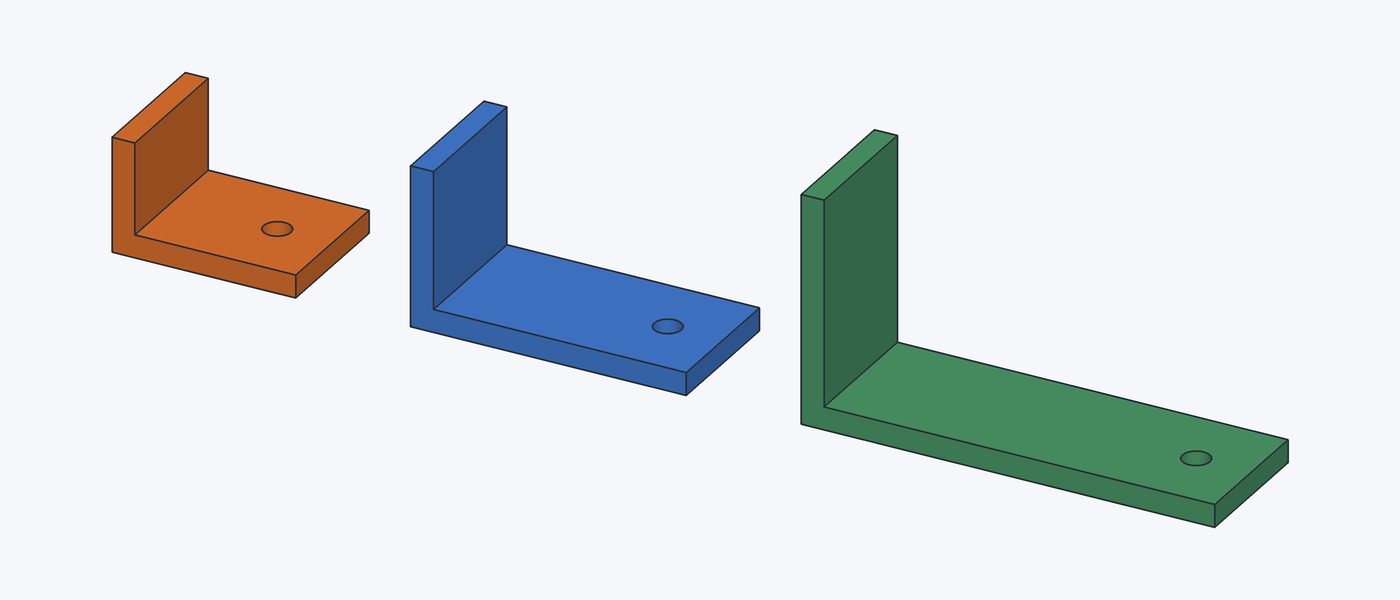
\includegraphics[width=0.32\linewidth]{fig/cfg_bracket.png}\hfill
  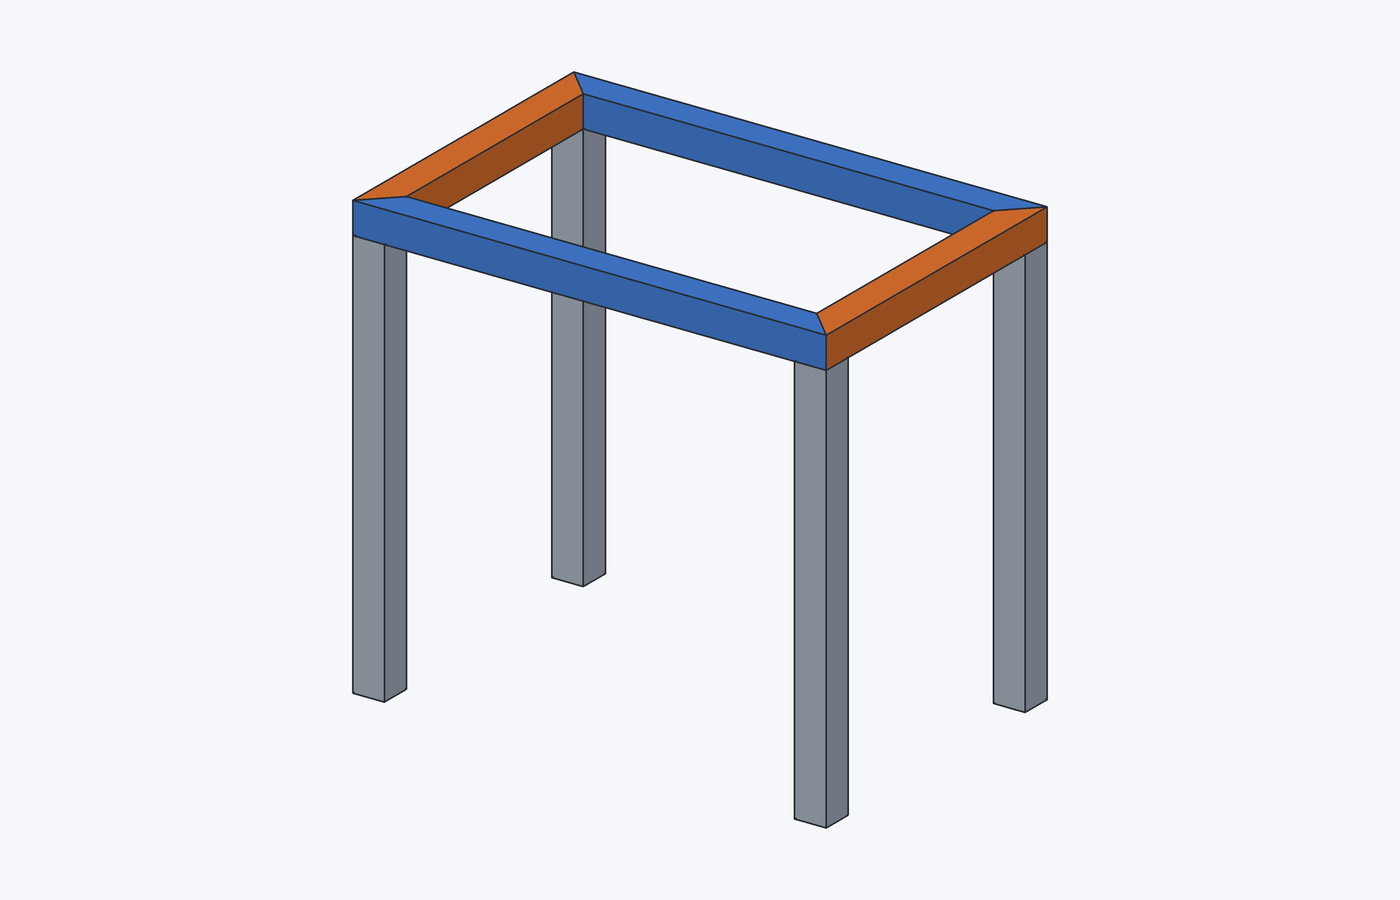
\includegraphics[width=0.32\linewidth]{fig/frame_weldment.png}\hfill
  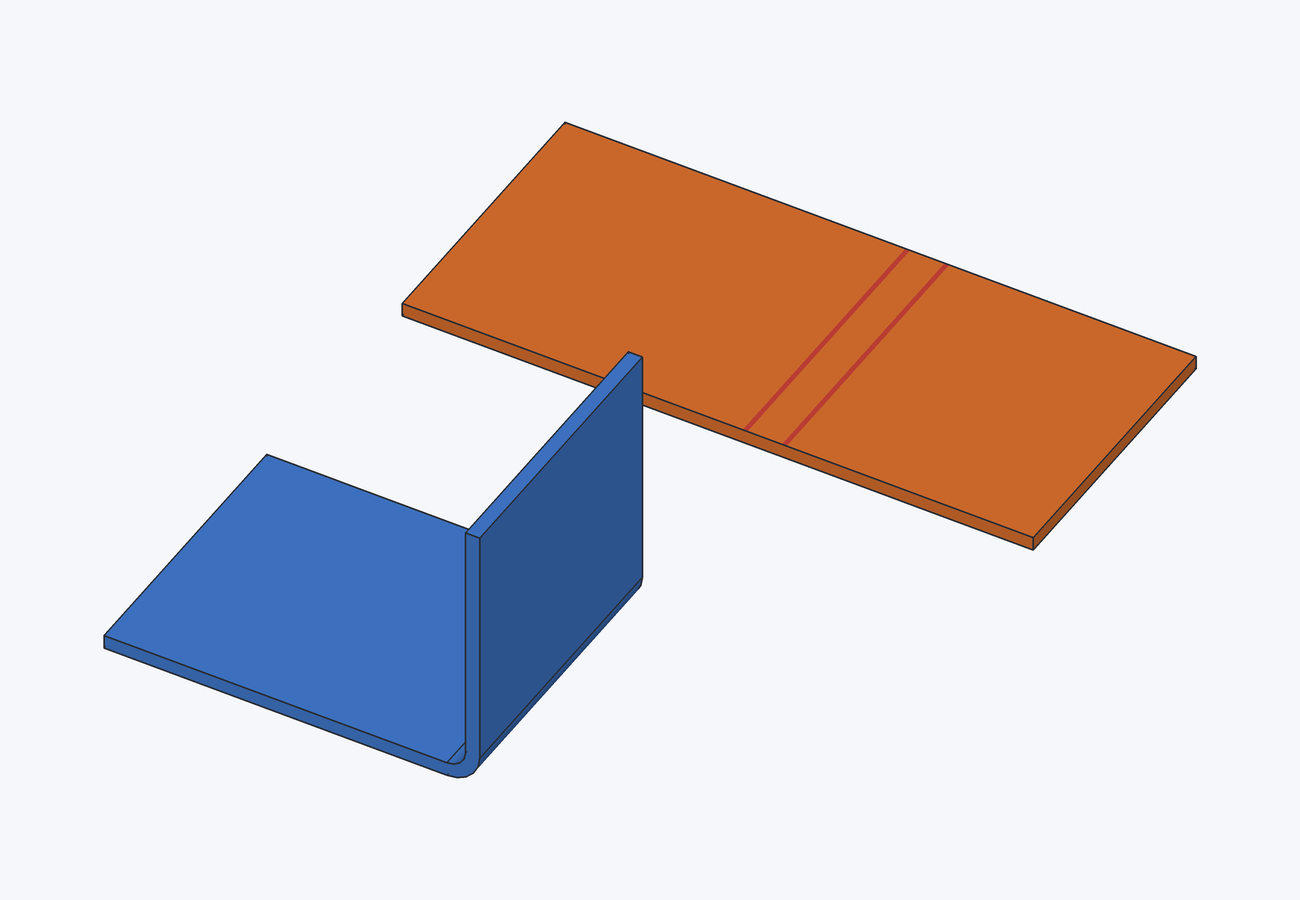
\includegraphics[width=0.32\linewidth]{fig/sheet_flat.png}\\[2pt]
  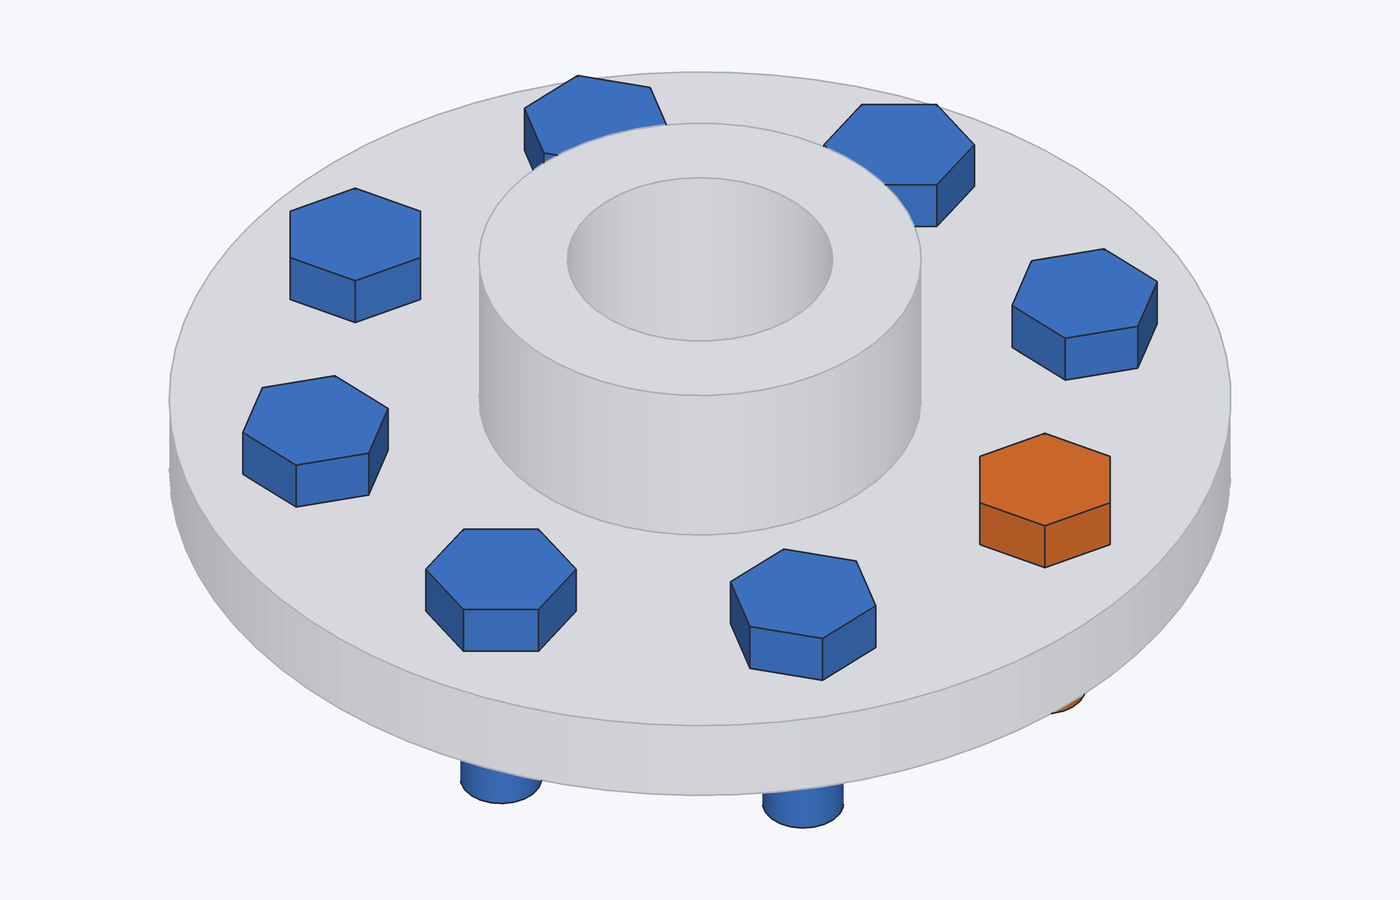
\includegraphics[width=0.32\linewidth]{fig/component_pattern.png}\hfill
  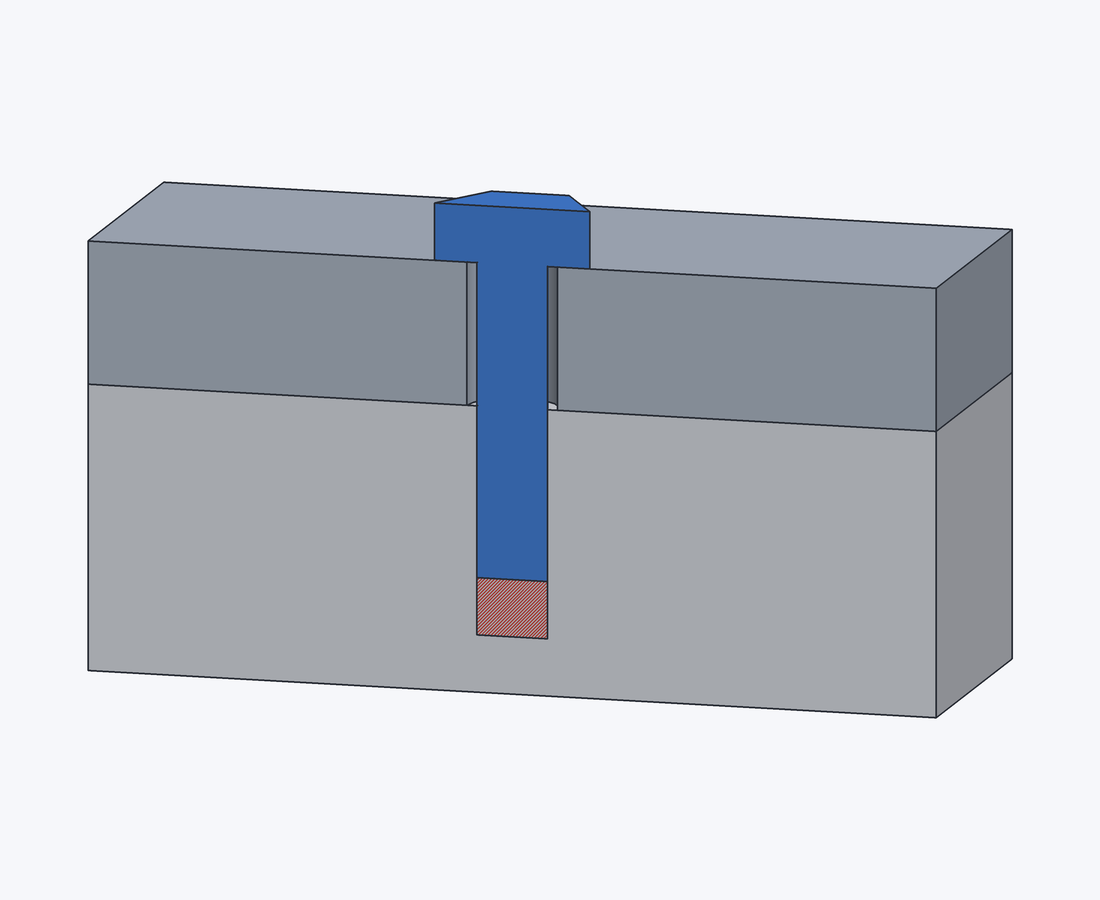
\includegraphics[width=0.32\linewidth]{fig/interference.png}\hfill
  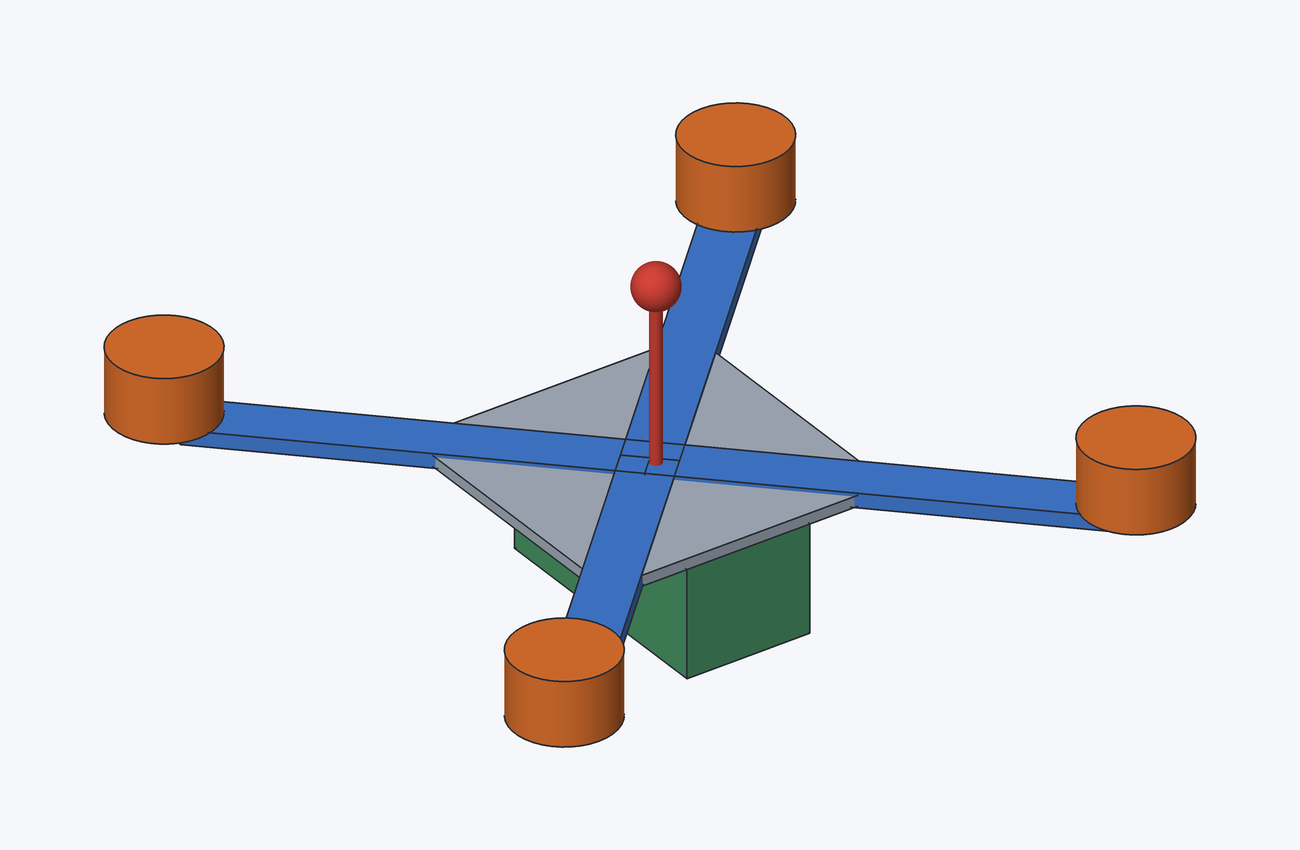
\includegraphics[width=0.32\linewidth]{fig/mass_cg.png}
  \end{center}
  {\small\color{bwgrey} All six models were built and recomputed in headless FreeCAD 1.1.4 by the scripts
  in \file{scripts/}. The renders are working figures; they will be regenerated after the UI redesign
  (\eref{UIX-09}).}
\end{titlepage}

\tableofcontents
\newpage

%======================================================================
\section{Summary}\label{sec:summary}
%======================================================================

\textbf{Goal.} BruceWorx (FreeCAD) reaches \emph{full parity with Fusion~360 and SolidWorks} across the
whole product lifecycle, so that it can become the CAD system of record for BruceWorx products. That covers
sketching and part modeling, assembly, simulation, ASME drawings, part and drawing management, and the
files sent to the 3D printer, the CNC shop and the laser cutter. This replaces the earlier position
(FC-T01) that FreeCAD only complements Fusion. The switch itself is the last milestone (M6) and is gated on the parity
matrix in Appendix~\ref{app:parity}.

\textbf{How this document was built.} The previous version of this file was a UI plan (Fusion-style
layout, patterns, command line). It is now one chapter's worth of material inside a roadmap with
\textbf{13 tracks and 87 epics}. The inputs were:
\begin{itemize}
  \item a five-round interview with you (18--19 Oct 2026), recorded in \S\ref{sec:decisions};
  \item the BruceWorx Ops ``work'' list (191 items, marked \emph{sample data}), used as \emph{ideas only}.
        Appendix~\ref{app:ideas} maps every idea group to the epic that absorbs it;
  \item a capability survey of FreeCAD~1.1.4 in this repository (grep of the actual sources and headless
        experiments), compared with Fusion~360 and SolidWorks~2026 public material;
  \item the repository's merged work (\code{[BW]} commits \#3--\#9), which marks four epics done and five in
        progress.
\end{itemize}

\textbf{Granularity.} The roadmap stops at \emph{epics}. Each epic has a scope, dependencies, an acceptance test and
the ideas it absorbs. Tasks are broken down when an epic starts. \file{roadmap-epics.csv} carries the same
87 epics for import into Ops. It is generated from \file{scripts/epics.py}, together with the tables in this
document, so the two cannot drift.

\textbf{Styling comes later.} The UI and styling track runs after M2. The figures here are working renders
and will be regenerated for the new UI (\eref{UIX-09}).

\subsection{Decisions from the interview}\label{sec:decisions}
\begin{center}
\small
\begin{longtable}{@{}p{3.6cm}p{12.4cm}@{}}
\toprule
Topic & Decision\\
\midrule\endhead
End state & Full Fusion~360 / SolidWorks parity; FreeCAD becomes system of record at M6\\
Ops task list & Ideas only; fresh IDs (\code{BW-\textit{TRK}-\textit{nn}}), origins kept in Appendix~\ref{app:ideas}\\
Manufacturing & FDM printing (PETG/ABS), CNC machining, sheet metal / laser. Not injection molding\\
First stage & Part and assembly modeling (main track)\\
Track order & Modeling/assembly first; \textbf{PDM evaluation and drawings run in parallel from the start}\\
Core modeling & Configurations; direct edit on imported STEP; parameters and top-down; threads and hardware\\
Advanced modeling & Freeform / T-spline-like; surfacing parity; mesh $\rightarrow$ solid; frames / weldments\\
File model & SolidWorks-style: \textbf{one file per part}, each with its own part number; assemblies link to files\\
Assembly extras & In-context editing; large-assembly mode; smart fastener mating; dynamic motion study\\
Simulation & Static + contact, modal and buckling, thermal and thermal stress. CFD later\\
FDM materials & Isotropic + knockdown by default; orthotropic by print orientation available per study\\
Drawing standard & ASME Y14.5, third-angle projection\\
Drawings & Associative BOM + balloons; GD\&T and datums with model-driven callouts; revision table and
  release; auto-generate drawing\\
PDM home & \textbf{Evaluate first} (Ops as PLM vs Ops + Git LFS vs in-FreeCAD vault vs open-source PLM)\\
Lifecycle & WIP $\rightarrow$ In Review $\rightarrow$ Released $\rightarrow$ Obsolete. Numeric pre-release
  revisions (01, 02, \ldots), letter at first release (A), then ECR $\rightarrow$ ECO for every later letter
  (ASME Y14.35 + SW-PDM practice)\\
Revision vs P/N & Revision is metadata, separate from the part number; drawings and packages print
  \code{P/N-REV}\\
Team & 2--5 concurrent editors: check-out locks, review and approval\\
Outputs & 3D-print prep; CNC CAM; sheet-metal flat DXF; release package\\
Kept idea areas & AI / MCP assistant; KiCad bridge; robotics and drone kits; kernel study\\
UI items & Patterns $\rightarrow$ Modeling; workspaces, panels, toolbar $\rightarrow$ UI track (later);
  command line $\rightarrow$ Automation\\
Upstream & \textbf{Track FreeCAD main} continuously (replaces ``stay on 1.1.4, rebase at 26.3'')\\
Deliverable & This document plus \file{roadmap-epics.csv}; epics only\\
Rule (standing) & Every feature is on by default, with an off switch on Preferences $\rightarrow$ BruceWorx\\
\bottomrule
\end{longtable}
\end{center}

\subsection{The lifecycle and where parity stands}

\begin{figure}[ht]
\centering
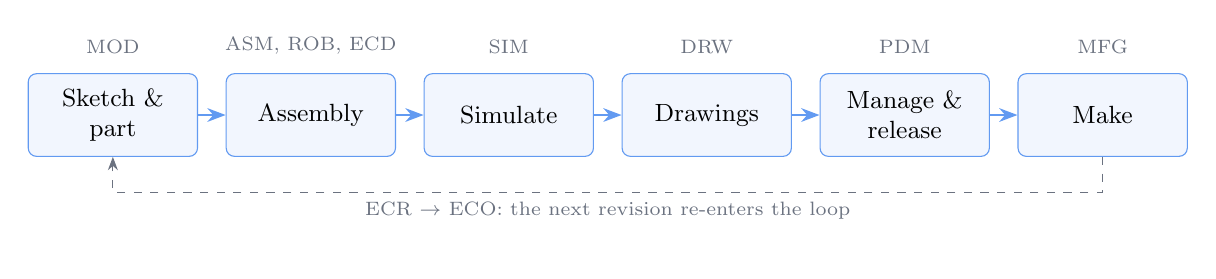
\begin{tikzpicture}[>=Stealth,
  st/.style={draw=bwblue!70,fill=bwblue!6,rounded corners=3pt,minimum width=2.15cm,minimum height=1.05cm,
             align=center,font=\small},
  lab/.style={font=\scriptsize\color{bwgrey},align=center}]
\node[st] (s1) {Sketch \&\\part};
\node[st,right=0.35cm of s1] (s2) {Assembly};
\node[st,right=0.35cm of s2] (s3) {Simulate};
\node[st,right=0.35cm of s3] (s4) {Drawings};
\node[st,right=0.35cm of s4] (s5) {Manage \&\\release};
\node[st,right=0.35cm of s5] (s6) {Make};
\foreach \a/\b in {s1/s2,s2/s3,s3/s4,s4/s5,s5/s6} \draw[->,thick,bwblue!70] (\a) -- (\b);
\draw[->,bwgrey,dashed] (s6.south) -- ++(0,-0.45) -| node[pos=0.25,below,lab]{ECR $\rightarrow$ ECO: the next revision re-enters the loop} (s1.south);
\node[lab,above=0.12cm of s1] {MOD};
\node[lab,above=0.12cm of s2] {ASM, ROB, ECD};
\node[lab,above=0.12cm of s3] {SIM};
\node[lab,above=0.12cm of s4] {DRW};
\node[lab,above=0.12cm of s5] {PDM};
\node[lab,above=0.12cm of s6] {MFG};
\node[lab,below=0.95cm of s1] {\phalf};
\node[lab,below=0.95cm of s2] {\phalf};
\node[lab,below=0.95cm of s3] {\phalf};
\node[lab,below=0.95cm of s4] {\phalf};
\node[lab,below=0.95cm of s5] {\pnone};
\node[lab,below=0.95cm of s6] {\phalf};
\end{tikzpicture}
\caption{Lifecycle stages, the tracks that serve them, and FreeCAD~1.1.4's overall standing against
Fusion/SolidWorks (\pfull{} full, \phalf{} partial, \pnone{} none). Part and drawing management is the only
stage with nothing in core FreeCAD. Foundation (FND), automation (AUT), UI (UIX) and kernel (KRN) cut across
all stages.}
\label{fig:lifecycle}
\end{figure}

The detailed matrix (Appendix~\ref{app:parity}, 71 capabilities) shows the pattern behind
Figure~\ref{fig:lifecycle}:
\begin{itemize}
  \item \textbf{Strong already:} parametric solids, joints and kinematic simulation (Assembly in 1.1),
        CalculiX/Elmer analysis types, drawing views, CAM and post-processors, 3MF and DXF export, Python.
  \item \textbf{Partial:} patterns (with a bug, \S\ref{sec:bug}), parameters, direct edit (Defeaturing only),
        surfacing, threads (drawing-side only), BOM (four automatic columns), GD\&T (symbol library, not
        semantic), mesh $\rightarrow$ solid (faceted).
  \item \textbf{Missing:} configurations, freeform, weldments, interference, smart fasteners, dynamic
        motion, safety-factor and orthotropic results, auto drawings, \emph{all} of PDM, slicer handoff,
        rendering, generative design.
\end{itemize}

\subsection{Milestones}

Milestones are \emph{gates}, not calendar dates. Tracks run in parallel. A milestone closes when all of its
epics pass acceptance on real BruceWorx parts. The Leonardo pedestal assembly \code{LE-02001} is the pilot
throughout.

\begin{center}
\small
\begin{tabularx}{\linewidth}{@{}lp{4.3cm}X@{}}
\toprule
& Milestone & Exit criterion\\
\midrule
M0 & Foundation green & CI green on Linux and macOS arm64; tagged release; nightly rebase on upstream main; review fixes in\\
M1 & Model it & LE-02001 modelled in FreeCAD from scratch: one file per part, patterns, configurations, threads, joints, interference-free\\
M2 & Document \& release it & LE-02001 rev A released \emph{from FreeCAD}: ASME drawings, BOM, PDM lifecycle, release package\\
M3 & Make it & Printed, machined and laser-cut parts made from FreeCAD outputs without touching Fusion\\
M4 & Validate it & Static, modal, buckling and thermal studies on LE parts, verified against benchmarks\\
M5 & Advanced & Surfacing, freeform, mesh $\rightarrow$ solid, in-context, large-assembly, dynamic motion, command line, assistant\\
M6 & Switch system of record & Parity matrix met for the LE scope; Fusion data migrated; FC-T01 criteria satisfied\\
UI & UI and styling pass & After M2: workspaces, panels, fresh visual design, regenerated figures\\
BG & Background & Kernel study; runs at low priority throughout\\
\bottomrule
\end{tabularx}
\end{center}

\begin{figure}[ht]
\centering
% Generated by scripts/epics.py; do not edit.
\begin{tabular}{@{}>{\raggedright\arraybackslash}p{2.35cm}*{9}{>{\centering\arraybackslash}p{1.12cm}}@{}}
\toprule
\textbf{Track} & \textbf{M0} & \textbf{M1} & \textbf{M2} & \textbf{M3} & \textbf{M4} & \textbf{M5} & \textbf{M6} & \textbf{UI} & \textbf{BG}\\
\midrule
\scriptsize Foundation \& upstream & \scriptsize \textcolor{bworange}{01} \textcolor{bworange}{02} \textcolor{bwdark}{03} \textcolor{bwdark}{04} \textcolor{bwdark}{05} \textcolor{bworange}{06} \textcolor{bwgreen}{07} &  &  &  &  &  &  &  & \\[2pt]
\scriptsize Part modeling &  & \scriptsize \textcolor{bworange}{01} \textcolor{bwdark}{02} \textcolor{bwdark}{03} \textcolor{bwdark}{04} \textcolor{bwdark}{05} \textcolor{bwdark}{11} \textcolor{bwdark}{12} &  & \scriptsize \textcolor{bwdark}{06} \textcolor{bwdark}{07} &  & \scriptsize \textcolor{bwdark}{08} \textcolor{bwdark}{09} \textcolor{bwdark}{10} &  &  & \\[2pt]
\scriptsize Assembly &  & \scriptsize \textcolor{bwdark}{01} \textcolor{bwgreen}{02} \textcolor{bworange}{03} \textcolor{bworange}{04} \textcolor{bwdark}{05} \textcolor{bwdark}{06} &  &  &  & \scriptsize \textcolor{bwdark}{07} \textcolor{bwdark}{08} \textcolor{bwdark}{09} \textcolor{bwdark}{10} &  &  & \\[2pt]
\scriptsize Drawings (ASME) &  &  & \scriptsize \textcolor{bwdark}{01} \textcolor{bwdark}{02} \textcolor{bwdark}{03} \textcolor{bwdark}{04} \textcolor{bwdark}{05} \textcolor{bwdark}{06} \textcolor{bwdark}{08} & \scriptsize \textcolor{bwdark}{07} &  &  &  &  & \\[2pt]
\scriptsize Part \& drawing management &  &  & \scriptsize \textcolor{bwgreen}{01} \textcolor{bworange}{02} \textcolor{bworange}{03} \textcolor{bwdark}{04} \textcolor{bwdark}{05} \textcolor{bwdark}{06} \textcolor{bwdark}{07} &  &  &  & \scriptsize \textcolor{bwdark}{08} &  & \\[2pt]
\scriptsize Simulation &  &  &  &  & \scriptsize \textcolor{bwdark}{01} \textcolor{bwdark}{02} \textcolor{bwdark}{03} \textcolor{bwdark}{04} \textcolor{bwdark}{05} & \scriptsize \textcolor{bwdark}{06} &  &  & \\[2pt]
\scriptsize Manufacturing outputs &  &  & \scriptsize \textcolor{bwdark}{04} & \scriptsize \textcolor{bwdark}{01} \textcolor{bwdark}{02} \textcolor{bwdark}{03} &  &  &  &  & \\[2pt]
\scriptsize Robotics \& drone kits &  & \scriptsize \textcolor{bwdark}{01} \textcolor{bwdark}{03} &  & \scriptsize \textcolor{bwdark}{02} \textcolor{bwdark}{04} &  & \scriptsize \textcolor{bwdark}{05} &  &  & \\[2pt]
\scriptsize ECAD bridge (KiCad) &  & \scriptsize \textcolor{bwdark}{01} &  & \scriptsize \textcolor{bwdark}{02} \textcolor{bwdark}{03} \textcolor{bwdark}{04} &  &  &  &  & \\[2pt]
\scriptsize Wire routing &  &  &  & \scriptsize \textcolor{bwdark}{01} \textcolor{bwdark}{02} \textcolor{bwdark}{03} \textcolor{bwdark}{04} &  & \scriptsize \textcolor{bwdark}{05} \textcolor{bwdark}{06} &  &  & \\[2pt]
\scriptsize AI \& automation & \scriptsize \textcolor{bwgreen}{01} & \scriptsize \textcolor{bwdark}{02} \textcolor{bwdark}{03} &  &  &  & \scriptsize \textcolor{bwdark}{04} \textcolor{bwdark}{05} &  &  & \\[2pt]
\scriptsize UI \& styling &  &  &  &  &  &  &  & \scriptsize \textcolor{bwgreen}{01} \textcolor{bwgreen}{02} \textcolor{bworange}{03} \textcolor{bworange}{04} \textcolor{bwdark}{05} \textcolor{bwdark}{06} \textcolor{bwdark}{07} \textcolor{bwdark}{08} \textcolor{bworange}{09} & \\[2pt]
\scriptsize Kernel study &  &  &  &  &  &  &  &  & \scriptsize \textcolor{bwdark}{01} \textcolor{bwdark}{02} \textcolor{bwdark}{03}\\[2pt]
\bottomrule
\end{tabular}

\caption{Epics by track and milestone (number = epic, e.g.\ Part modeling \code{03} = \eref{BW-MOD-03}).
Colour shows status: \textcolor{bwgreen}{\textbf{done}}, \textcolor{bworange}{\textbf{in progress}}, to do.
Generated from \file{scripts/epics.py}.}
\label{fig:swim}
\end{figure}

\subsection{Critical path}

\begin{figure}[ht]
\centering
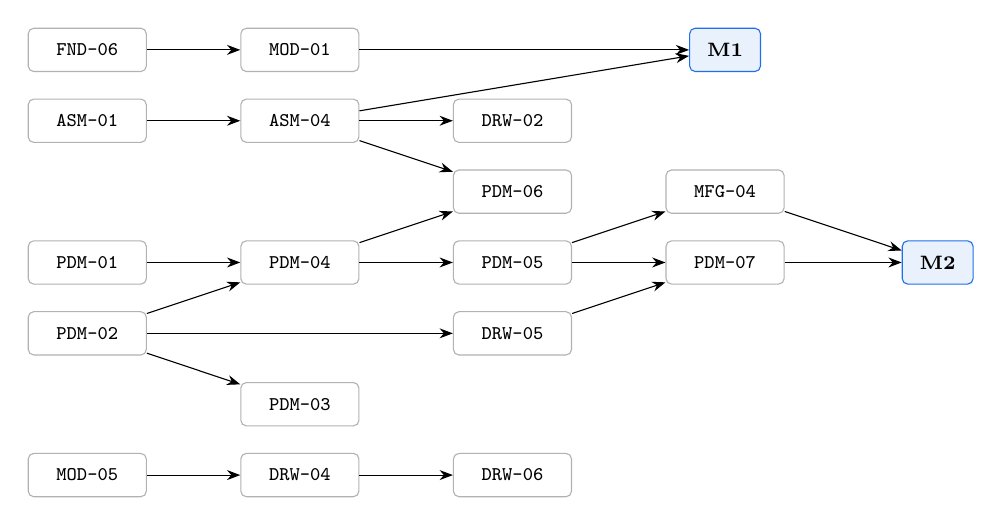
\begin{tikzpicture}[>=Stealth,x=2.7cm,y=-0.9cm,
  e/.style={draw=black!30,rounded corners=2pt,fill=white,font=\scriptsize\ttfamily,minimum width=1.5cm,minimum height=0.55cm},
  m/.style={draw=bwblue,fill=bwblue!10,rounded corners=2pt,font=\scriptsize\bfseries,minimum width=0.9cm,minimum height=0.55cm}]
\node[e] (f6) at (0,0) {FND-06};  \node[e] (m1) at (1,0) {MOD-01};  \node[m] (M1) at (3,0) {M1};
\node[e] (a1) at (0,1) {ASM-01};  \node[e] (a4) at (1,1) {ASM-04};  \node[e] (d2) at (2,1) {DRW-02};
\node[e] (p6) at (2,2) {PDM-06};  \node[e] (o4) at (3,2) {MFG-04};
\node[e] (p1) at (0,3) {PDM-01};  \node[e] (p4) at (1,3) {PDM-04};  \node[e] (p5) at (2,3) {PDM-05};
\node[e] (p7) at (3,3) {PDM-07};  \node[m] (M2) at (4,3) {M2};
\node[e] (p2) at (0,4) {PDM-02};  \node[e] (d5) at (2,4) {DRW-05};
\node[e] (p3) at (1,5) {PDM-03};
\node[e] (m5) at (0,6) {MOD-05};  \node[e] (d4) at (1,6) {DRW-04};  \node[e] (d6) at (2,6) {DRW-06};
\draw[->] (f6) -- (m1); \draw[->] (m1) -- (M1); \draw[->] (a4) -- (M1);
\draw[->] (a1) -- (a4); \draw[->] (a4) -- (d2); \draw[->] (a4) -- (p6); \draw[->] (p4) -- (p6);
\draw[->] (p1) -- (p4); \draw[->] (p2) -- (p4); \draw[->] (p2) -- (p3); \draw[->] (p2) -- (d5);
\draw[->] (p4) -- (p5); \draw[->] (p5) -- (p7); \draw[->] (d5) -- (p7); \draw[->] (p5) -- (o4);
\draw[->] (p7) -- (M2); \draw[->] (o4) -- (M2);
\draw[->] (m5) -- (d4); \draw[->] (d4) -- (d6);
\end{tikzpicture}
\caption{The dependencies that decide when FreeCAD can release a documented assembly (M2). The PDM
evaluation (\eref{PDM-01}) and data model (\eref{PDM-02}) have no prerequisites, which is why they start on
day one alongside modeling.}
\label{fig:critical}
\end{figure}

\subsection{All epics}
\small
% Generated by scripts/epics.py; do not edit.
\begin{longtable}{@{}p{1.4cm}p{5.8cm}p{0.9cm}p{4.3cm}p{1.95cm}@{}}
\toprule ID & Epic & Mile. & Depends on & Status\\ \midrule\endhead
\bottomrule\endfoot
\midrule\multicolumn{5}{@{}l}{\textbf{Foundation \& upstream}}\\
\code{FND-01} & Build \& CI on Linux and macOS arm64 & M0 & --- & \stProg\\
\code{FND-02} & Packaging, branding \& releases & M0 & \scriptsize FND-01 & \stProg\\
\code{FND-03} & Track upstream FreeCAD main & M0 & \scriptsize FND-01 & \stTodo\\
\code{FND-04} & Licences \& notices & M0 & --- & \stTodo\\
\code{FND-05} & Acceptance corpus \& test harness & M0 & --- & \stTodo\\
\code{FND-06} & Fixes found in review & M0 & --- & \stProg\\
\code{FND-07} & On by default, each with an off switch & M0 & --- & \stDone\\
\midrule\multicolumn{5}{@{}l}{\textbf{Part modeling}}\\
\code{MOD-01} & Rectangular \& circular patterns & M1 & \scriptsize FND-06 & \stProg\\
\code{MOD-02} & Parameters \& top-down design & M1 & --- & \stTodo\\
\code{MOD-03} & Configurations & M1 & \scriptsize MOD-02 & \stTodo\\
\code{MOD-04} & Direct edit on imported geometry & M1 & --- & \stTodo\\
\code{MOD-05} & Threads, holes \& hardware library & M1 & --- & \stTodo\\
\code{MOD-06} & Sheet metal & M3 & --- & \stTodo\\
\code{MOD-07} & Frames \& weldments & M3 & --- & \stTodo\\
\code{MOD-08} & Surfacing parity & M5 & --- & \stTodo\\
\code{MOD-09} & Freeform (subdivision / T-spline-like) & M5 & \scriptsize MOD-08 & \stTodo\\
\code{MOD-10} & Mesh to solid & M5 & --- & \stTodo\\
\code{MOD-11} & Inspect tools & M1 & --- & \stTodo\\
\code{MOD-12} & Sketcher parity audit & M1 & --- & \stTodo\\
\midrule\multicolumn{5}{@{}l}{\textbf{Assembly}}\\
\code{ASM-01} & File model: one part per file & M1 & --- & \stTodo\\
\code{ASM-02} & Assembly gap audit & M1 & --- & \stDone\\
\code{ASM-03} & Joint UX \& limits & M1 & \scriptsize ASM-02 & \stProg\\
\code{ASM-04} & Exploded views \& BOM & M1 & \scriptsize ASM-01 & \stProg\\
\code{ASM-05} & Sub-assemblies & M1 & \scriptsize ASM-01 & \stTodo\\
\code{ASM-06} & Interference \& clearance & M1 & --- & \stTodo\\
\code{ASM-07} & In-context editing & M5 & \scriptsize ASM-01 MOD-02 & \stTodo\\
\code{ASM-08} & Large-assembly mode & M5 & \scriptsize ASM-01 & \stTodo\\
\code{ASM-09} & Smart fastener mating & M5 & \scriptsize MOD-05 ASM-03 & \stTodo\\
\code{ASM-10} & Dynamic motion study & M5 & \scriptsize ASM-03 & \stTodo\\
\midrule\multicolumn{5}{@{}l}{\textbf{Drawings (ASME)}}\\
\code{DRW-01} & ASME templates \& title block & M2 & --- & \stTodo\\
\code{DRW-02} & Associative BOM table \& balloons & M2 & \scriptsize ASM-04 & \stTodo\\
\code{DRW-03} & GD\&T \& datums (ASME Y14.5) & M2 & --- & \stTodo\\
\code{DRW-04} & Hole \& thread callouts from the model & M2 & \scriptsize MOD-05 & \stTodo\\
\code{DRW-05} & Revision table \& release stamp & M2 & \scriptsize PDM-02 & \stTodo\\
\code{DRW-06} & Auto-generate drawing & M2 & \scriptsize DRW-01 DRW-04 & \stTodo\\
\code{DRW-07} & Sheet-metal flat \& cut-list drawings & M3 & \scriptsize MOD-06 MOD-07 & \stTodo\\
\code{DRW-08} & Publish PDF/DXF & M2 & \scriptsize DRW-01 & \stTodo\\
\midrule\multicolumn{5}{@{}l}{\textbf{Part \& drawing management}}\\
\code{PDM-01} & PDM evaluation \& decision & M2 & --- & \stDone\\
\code{PDM-02} & Data model \& lifecycle spec & M2 & --- & \stProg\\
\code{PDM-03} & Numbering service & M2 & \scriptsize PDM-02 & \stProg\\
\code{PDM-04} & FreeCAD vault client & M2 & \scriptsize PDM-01 PDM-02 & \stTodo\\
\code{PDM-05} & Lifecycle \& change control & M2 & \scriptsize PDM-04 & \stTodo\\
\code{PDM-06} & BOM sync \& where-used & M2 & \scriptsize ASM-04 PDM-04 & \stTodo\\
\code{PDM-07} & Pilot: LE-02001 \& CAD register & M2 & \scriptsize PDM-05 DRW-05 & \stTodo\\
\code{PDM-08} & Migration from Fusion & M6 & \scriptsize PDM-07 & \stTodo\\
\midrule\multicolumn{5}{@{}l}{\textbf{Simulation}}\\
\code{SIM-01} & Study setup (Fusion-style) & M4 & --- & \stTodo\\
\code{SIM-02} & Contacts, bolts \& preload & M4 & \scriptsize SIM-01 & \stTodo\\
\code{SIM-03} & Materials incl. FDM & M4 & \scriptsize SIM-01 & \stTodo\\
\code{SIM-04} & Results \& reports & M4 & \scriptsize SIM-01 & \stTodo\\
\code{SIM-05} & Verification benchmarks & M4 & \scriptsize SIM-01 & \stTodo\\
\code{SIM-06} & CFD / airflow (later) & M5 & \scriptsize SIM-01 & \stTodo\\
\midrule\multicolumn{5}{@{}l}{\textbf{Manufacturing outputs}}\\
\code{MFG-01} & 3D-print prep & M3 & \scriptsize MOD-11 & \stTodo\\
\code{MFG-02} & CNC CAM & M3 & --- & \stTodo\\
\code{MFG-03} & Sheet-metal flat DXF & M3 & \scriptsize MOD-06 & \stTodo\\
\code{MFG-04} & Release package & M2 & \scriptsize PDM-05 DRW-08 & \stTodo\\
\midrule\multicolumn{5}{@{}l}{\textbf{Robotics \& drone kits}}\\
\code{ROB-01} & COTS library \& insert & M1 & \scriptsize MOD-05 & \stTodo\\
\code{ROB-02} & Frame \& arm templates & M3 & \scriptsize MOD-03 & \stTodo\\
\code{ROB-03} & Mass, CG \& inertia report & M1 & \scriptsize MOD-11 ROB-01 & \stTodo\\
\code{ROB-04} & Drone balance \& thrust-to-weight & M3 & \scriptsize ROB-03 & \stTodo\\
\code{ROB-05} & Kinematic chains \& joint drive & M5 & \scriptsize ASM-03 & \stTodo\\
\midrule\multicolumn{5}{@{}l}{\textbf{ECAD bridge (KiCad)}}\\
\code{ECD-01} & ECAD intake \& adopt-vs-build & M1 & --- & \stTodo\\
\code{ECD-02} & Board STEP into assembly & M3 & \scriptsize ECD-01 & \stTodo\\
\code{ECD-03} & Board outline round-trip & M3 & \scriptsize ECD-01 & \stTodo\\
\code{ECD-04} & Placement sync \& enclosure fit & M3 & \scriptsize ECD-02 ASM-06 & \stTodo\\
\midrule\multicolumn{5}{@{}l}{\textbf{Wire routing}}\\
\code{WIR-01} & Adopt versus build & M3 & --- & \stTodo\\
\code{WIR-02} & Port and wire & M3 & \scriptsize WIR-01 & \stTodo\\
\code{WIR-03} & Assembly follow & M3 & \scriptsize WIR-02 ASM-03 & \stTodo\\
\code{WIR-04} & From-to cut list & M3 & \scriptsize WIR-02 ASM-04 & \stTodo\\
\code{WIR-05} & Clips and bundles & M5 & \scriptsize WIR-03 & \stTodo\\
\code{WIR-06} & Route on the clip graph & M5 & \scriptsize WIR-05 & \stTodo\\
\midrule\multicolumn{5}{@{}l}{\textbf{AI \& automation}}\\
\code{AUT-01} & Headless hooks \& CLI & M0 & --- & \stDone\\
\code{AUT-02} & bruceworx.api & M1 & \scriptsize AUT-01 & \stTodo\\
\code{AUT-03} & MCP server & M1 & \scriptsize AUT-02 & \stTodo\\
\code{AUT-04} & Assistant panel & M5 & \scriptsize AUT-03 & \stTodo\\
\code{AUT-05} & Command line & M5 & --- & \stTodo\\
\midrule\multicolumn{5}{@{}l}{\textbf{UI \& styling}}\\
\code{UIX-01} & Theme, pref pack \& viewport styling & UI & --- & \stDone\\
\code{UIX-02} & macOS title bar & UI & --- & \stDone\\
\code{UIX-03} & Browser (overlay model tree) & UI & --- & \stProg\\
\code{UIX-04} & History timeline & UI & --- & \stProg\\
\code{UIX-05} & Workspaces \& tabs (Fusion naming) & UI & --- & \stTodo\\
\code{UIX-06} & Toolbar \& panels & UI & \scriptsize UIX-05 & \stTodo\\
\code{UIX-07} & Task panel polish & UI & --- & \stTodo\\
\code{UIX-08} & Matcap shading & UI & --- & \stTodo\\
\code{UIX-09} & Fresh UI design \& re-render figures & UI & \scriptsize UIX-05 & \stProg\\
\midrule\multicolumn{5}{@{}l}{\textbf{Kernel study}}\\
\code{KRN-01} & OCCT coupling survey & BG & --- & \stTodo\\
\code{KRN-02} & STEP exchange harness & BG & \scriptsize FND-05 & \stTodo\\
\code{KRN-03} & Kernel decision & BG & \scriptsize KRN-01 KRN-02 & \stTodo\\
\end{longtable}

\normalsize

%======================================================================
\section{Test session --- Sunday 19 October 2026 (tonight)}\label{sec:tonight}
%======================================================================

\textbf{What is being tested.} The first build with roadmap work in it: the review fixes (\eref{FND-06}) and
Rectangular/Circular Pattern for bodies and components (\eref{MOD-01}). Everything below already passes headless
(171 PartDesign tests, 19 pattern tests, offscreen dialog and observer checks; steps 14--17 were added with the
assembly audit and the part-property schema). Tonight is about what only a person
at the screen can judge: does it look right, feel right, and survive real clicking?

\begin{center}
\small
\begin{tabularx}{\linewidth}{@{}lX@{}}
\toprule
Branch & \code{bw/fnd06-mod01-patterns} (uncommitted; base \code{696260b})\\
Build & \file{build/release} (FreeCAD 1.1.4-bw.1), already rebuilt\\
Launch & \code{pixi run freecad-release} \quad (uses \file{package/bruceworx/run-freecad.sh})\\
Keep open & View $\rightarrow$ Panels $\rightarrow$ Report view, so warnings show up\\
\bottomrule
\end{tabularx}
\end{center}

\newcommand{\tick}{\tikz[baseline=-0.6ex]\draw[black!50] (0,-0.9ex) rectangle (1.8ex,0.9ex);}

\begin{center}
\small
\begin{longtable}{@{}p{0.5cm}p{6.4cm}p{6.6cm}c@{}}
\toprule
\# & Do & Expect & OK\\
\midrule\endhead
\bottomrule\endfoot
1 & Start FreeCAD. Look at the left side of the window before moving the mouse there. &
  The model tree (Browser) is visible without hovering. \emph{Fix: auto-hide now defaults to off.} & \tick\\
2 & Check the workbench tabs. \emph{Needs your pending \code{param\_fallback} fix, which is in the working tree.} &
  Only the trimmed set (PartDesign, Assembly, Sketcher, Part, TechDraw, Draft, Spreadsheet, Start); the Report
  view shows ``BruceWorx: applied the BruceWorx preference pack''. & \tick\\
3 & PartDesign: a body with a 10\,mm box; Linear Pattern, direction 1 = X, 4 instances, spacing 10; direction 2 = Y,
  3 instances, spacing 10. & 12 boxes as one $40\times30\times10$ solid. Before the fix this gave 8. & \tick\\
4 & Open an old file that has a two-direction linear pattern (if you have one). & It now shows every row; the
  pattern repairs itself on recompute. & \tick\\
5 & Select a \emph{body} (not a feature) $\rightarrow$ Rectangular Pattern (PartDesign toolbar, after Polar Pattern,
  or BruceWorx menu). Change quantity, distance, distance type, Symmetric, then tick Direction~2. &
  Dialog opens with live preview; every change updates the 3D view at once; parallel directions show a red
  message instead of breaking. & \tick\\
6 & In the same dialog, uncheck two rows in ``Instances''. Press Cancel. Repeat and press OK. &
  Unchecked instances disappear. Cancel leaves no trace in the tree; OK leaves one ``\ldots pattern'' object. & \tick\\
7 & Select that pattern object and press Rectangular Pattern again. & The dialog reopens with the saved values and
  suppressed rows; edits apply to the same object. & \tick\\
8 & Move the original body (Transform or Placement). & The pattern follows. & \tick\\
9 & Select a body $\rightarrow$ Circular Pattern. Select a circular edge of a hole on another part, press
  ``Use selection'' next to Axis. Try Full, Angle 90\,$^\circ$, Symmetric. &
  Instances spin about that hole's centre; Angle and Symmetric spread as labelled; the angle box is greyed out for
  Full. & \tick\\
10 & Assembly: insert a bolt part, select it, Circular Pattern, quantity 6, OK. Then add a joint to one of the
  generated bolts. & Six bolts; the BOM / component count sees 6. \emph{Joint to a generated
  instance is the one case not tested headless.} & \tick\\
11 & Repeat 5 with Copies = Independent, OK. & Separate solids (bodies) or separate links (components) appear; they
  no longer follow the original. & \tick\\
12 & Select a PartDesign \emph{feature} (e.g.\ a pocket) $\rightarrow$ Rectangular Pattern. & PartDesign's own Linear
  Pattern dialog opens (features keep using PartDesign until the upstream rebase). & \tick\\
13 & Preferences $\rightarrow$ BruceWorx: untick ``Rectangular and Circular Pattern commands'', switch workbench. &
  The two buttons disappear from the toolbars. & \tick\\
\midrule
\multicolumn{4}{@{}p{14.6cm}@{}}{\textit{Added after the assembly audit (section~\ref{sec:asm-audit}); steps 14 and 16 test the joint
  changes of section~\ref{sec:joints}.}}\\
14 & Assembly: two parts joined by a Revolute joint, no limits. \emph{Drag}: click the moving part in the 3D view and
  pull it round. Then edit the joint: tick Min and Max angle, set 0 and 90\,$^\circ$, press \emph{Pick datums} and
  click a flat face on each part; OK. Drag again. &
  Without limits it swings all the way round. With them the panel shows ``Now at \ldots'' measured between the two
  faces, and the drag stops at 0 and 90\,$^\circ$ from where the faces line up. & \tick\\
15 & After step 10: change the bolt pattern quantity from 6 to 8, then to 4 (keep the jointed bolt within the
  first 4). Then to 2, so the jointed bolt goes away. &
  The joint stays on its bolt at 8 and 4. At 2 the joint reports a clear error in the tree, no crash. & \tick\\
16 & Put two parts where you want them by hand (Transform). Ground one. Add a Fixed joint between a face of each,
  first with \emph{Keep parts where they are} unticked, then tick it before OK. &
  Unticked: the second part jumps so the picked faces line up. Ticked: it goes back and stays exactly where you put
  it. & \tick\\
17 & Part properties: open the Python console (View $\rightarrow$ Panels) on a part file and run
  \newline\code{from bruceworx.partprops import load\_schema}\newline\code{load\_schema().apply(}\newline\code{\ \ App.ActiveDocument.Part)}\newline then give the
  body a material. In an assembly of it, Create BOM and add columns \code{.PartNumber}, \code{.Revision},
  \code{.MaterialName}, \code{.Mass}. &
  A ``BruceWorx'' group in the part's properties (P/N, Revision, Material name and Mass greyed out). The BOM shows
  the material and the mass; a revision typed as 01 shows as 01, not 1. & \tick\\
\end{longtable}
\end{center}

\paragraph{Report back.} For anything that is not as expected: a screenshot, the Report view text, and the step
number. Saving the test document (\code{File $\rightarrow$ Save}) helps reproduce it here.

\paragraph{Not in tonight's build.} Symmetric and suppression for PartDesign \emph{features} (they come with the
upstream rebase, \eref{FND-03}); the Fusion-style workspaces and panels (UI track, after M2).

%======================================================================
\section{Track FND --- Foundation and upstream}\label{sec:fnd}
%======================================================================

Every other track depends on a fork that builds reproducibly, ships, and keeps up with FreeCAD. Two
foundation decisions changed in the interview. BruceWorx now tracks \textbf{upstream main} instead of
waiting for the 26.3 tag. Fixes found while reviewing the UI now have an epic of their own.

\begin{epic}{FND-01}{Build \& CI on Linux and macOS arm64}{M0}{\stProg}{FCB-P0-CI-01..06, P0-01, P0-06..08, P0-10}
Pixi environments and lockfiles for both platforms, ccache in CI, and the self-hosted Apple-silicon runner.
\file{BUILDING-BRUCEWORX.md} and \file{.github/workflows/bruceworx-ci.yml} exist, and the Linux STEP check
and hosted macOS lock are merged (\#4).
\emph{Acceptance:} a fresh clone builds on both platforms using only the documented commands, and CI is green
on both.
\end{epic}

\begin{epic}{FND-02}{Packaging, branding \& releases}{M0}{\stProg}{FCB-P0-02, P0-03, P0-09, P0-11, P0-17, P0-18}
The version string already reads \code{1.1.4-bw.1}, and the unsigned arm64 \code{.dmg} script is merged
(\#3). Remaining: tag a release carrying the dmg plus a source tarball, and decide on signing and
notarisation before anyone outside the team installs it.
\emph{Acceptance:} the tagged release installs on a clean Mac and opens a Fusion STEP export
(\code{LE-01001}, 200$\times$200$\times$8 envelope).
\end{epic}

\begin{epic}{FND-03}{Track upstream FreeCAD main}{M0}{\stTodo}{FCB-P1-16..21, P0-12 (replaced)}
\file{UPSTREAM-SYNC.md} currently says ``stay on 1.1.4, rebase onto 26.3 when it ships''. That changes to
continuous tracking:
\begin{itemize}
  \item \code{upstream-main} stays a fast-forward mirror. A nightly job rebases the \code{[BW]} series onto it
        and runs the BruceWorx tests plus the headless acceptance corpus (\eref{FND-05}).
  \item A conflict or red build opens an issue automatically. The \emph{conflict budget} is the number of
        upstream files our series touches. It is reported each night and must not grow without a reason
        recorded in the PR.
  \item Product releases are still cut from a tested point (\code{main} after a green nightly), not from
        arbitrary upstream commits.
\end{itemize}
\emph{Why:} the Assembly, TechDraw and FEM work that parity depends on lands upstream continuously.
Rebasing once a year makes every conflict expensive at once.
\emph{Acceptance:} the nightly rebase runs for two weeks; each conflict is resolved within a working day.
\end{epic}

\begin{epic}{FND-04}{Licences \& notices}{M0}{\stTodo}{FCB-P0-13}
FreeCAD is LGPL-2.1-or-later. The roadmap bundles more components: SheetMetal (LGPL-2.1-or-later), OCP, CadQuery and build123d
(Apache-2.0), possibly an OpenSCAD binary (GPL-2, shipped as a separate executable) and a fastener library
(licence to check \verify). Each needs a line in \file{NOTICE} and a third-party licence file in the app
bundle.
\emph{Acceptance:} every bundled component is listed; each release has a source tarball attached.
\end{epic}

\begin{epic}{FND-05}{Acceptance corpus \& test harness}{M0}{\stTodo}{FCB-P1-09, P3-08}
One corpus serves every epic: native and STEP versions of LE parts and assemblies, the 2-DOF arm, the quad
frame, and the benchmark models in this document. A single command runs every headless check.
Screenshots come from the existing before/after script. The renders in this document already come from
headless FreeCAD (\file{scripts/}), and the harness generalises that.
\emph{Acceptance:} \code{pixi run acceptance} runs all checks in CI in under 15 minutes.
\end{epic}

\begin{epic}{FND-06}{Fixes found in review}{M0}{\stProg}{(new)}
\begin{enumerate}
  \item \textbf{Linear Pattern direction 2 drops a row} (\S\ref{sec:bug}). \code{Spacings2} is declared
        \code{(\{\})}, which stores \code{[0.0]}. Fix the declaration, migrate saved files, add a test.
  \item \textbf{Workbench trim not applied.} The pack lists FEM, CAM, BIM, Robot and others as disabled
        (\file{bruceworx\_pack.py:118}), but the screenshot shows 13 tabs. The uncommitted
        \code{param\_fallback} change suggests the pack crashed on \code{int(None)} \verify.
  \item \textbf{Overlay model tree missing} on the screenshot, although it is on by default; root cause unknown \verify.
\end{enumerate}
\emph{Acceptance:} a $4\times3$ pattern gives 12 instances; only intended workbenches are visible; the tree shows on first run.
\end{epic}

\begin{epic}{FND-07}{On by default, each with an off switch}{M0}{\stDone}{FCB-P1-01, P1-10}
Merged in \#9. It remains a rule for every epic below: a feature ships enabled and can be switched off on
Preferences~$\rightarrow$~BruceWorx, and switching it off restores stock behaviour.
\end{epic}

%======================================================================
\section{Track MOD --- Part modeling}\label{sec:mod}
%======================================================================

Modeling is the main track and comes first. M1 needs \eref{MOD-01}--\eref{MOD-05}, \eref{MOD-11} and
\eref{MOD-12}. Sheet metal and frames serve M3. Surfacing, freeform and mesh conversion are M5.

\begin{center}
\small
\begin{tabularx}{\linewidth}{@{}p{3.3cm}p{5.2cm}X@{}}
\toprule
Capability & FreeCAD 1.1.4 today (checked in this repo) & Gap to Fusion / SolidWorks\\
\midrule
Feature patterns & \code{LinearPattern} (2 directions), \code{PolarPattern}, \code{MultiTransform} & Bug in direction 2; no symmetric, no suppress\\
Body/component patterns & Draft link arrays & Not assembly-aware; no Fusion options\\
Parameters & Spreadsheet, \code{App::VarSet}, expressions & No Change Parameters dialog\\
Top-down & \code{ShapeBinder}, \code{SubShapeBinder} (cross-document) & No skeleton/derive workflow\\
Configurations & none (no configuration table in \file{src/Mod/Spreadsheet} or \file{src/App}) & Missing\\
Direct edit & \code{Part\_Defeaturing} (delete faces) & No press-pull, move or replace face\\
Threads & \code{Hole} has \code{ModelThread}; TechDraw draws cosmetic threads on views & No model-level cosmetic thread\\
Sheet metal & add-on only & Bundle (decided)\\
Weldments & none in core & Missing\\
Surfacing & Surface WB: Filling, Sections, GeomFillSurface, ExtendFace, BlendCurve; Part: Ruled, Offset, Thickness & Trim/untrim, stitch, continuity analysis\\
Freeform & none & Missing\\
Mesh $\rightarrow$ solid & \code{Part\_ShapeFromMesh} (faceted), ReverseEngineering WB & No segmentation/rebuild\\
Inspect & Measure incl.\ \code{MeasureCOM}; \code{Part\_CheckGeometry} & No overhang/draft/thickness maps\\
\bottomrule
\end{tabularx}
\end{center}

%----------------------------------------------------------------------
\subsection{BW-MOD-01 --- Rectangular and circular patterns}\label{sec:patterns}
%----------------------------------------------------------------------

\begin{epic}{MOD-01}{Rectangular \& circular patterns}{M1}{\stProg}{(new, from the UI plan)}
Two commands under \textsc{Create}: Rectangular Pattern and Circular Pattern. Each works on features,
bodies and assembly components, with Fusion's options: symmetric direction, suppress instances, and linked
vs.\ independent copies (linked by default). Depends on \eref{FND-06} (the direction-2 fix).
\emph{Acceptance:} Figures~\ref{fig:examples} and \ref{fig:new} reproduced in the GUI; undo/redo;
save/reload; the Assembly workbench sees every component instance.
\end{epic}

\begin{center}
\small
\begin{tabularx}{\linewidth}{@{}p{3.4cm}XX@{}}
\toprule
Fusion option & FreeCAD 1.1 today & Plan\\
\midrule
Pattern type: Features & PartDesign \code{LinearPattern} (2 directions), \code{PolarPattern} & Wrap these, fix the direction-2 bug\\
Pattern type: Bodies & Draft \code{make\_ortho\_array} / \code{make\_polar\_array} with \code{use\_link} & New command builds a link array, or copies\\
Pattern type: Components & Assembly understands link arrays (\file{UtilsAssembly.py:127--131}) & New command builds an \code{App::Link} array inside the assembly\\
Distance type: Extent / Spacing & \code{Mode} = Extent / Spacing & Same\\
Direction type: Symmetric & --- & \textbf{New}: index range $-\lfloor\frac{n-1}{2}\rfloor..\lceil\frac{n-1}{2}\rceil$\\
Circular type: Full / Angle / Symmetric & Angle + Extent/Spacing & Map Full/Angle; \textbf{new} Symmetric\\
Suppress instances & --- (features) & \textbf{New} for features; links: \code{setElementVisible}\\
Linked / independent & n/a & Dialog option (bodies, components)\\
\bottomrule
\end{tabularx}
\end{center}

\begin{figure}[ht]
\centering
\begin{subfigure}{0.49\linewidth}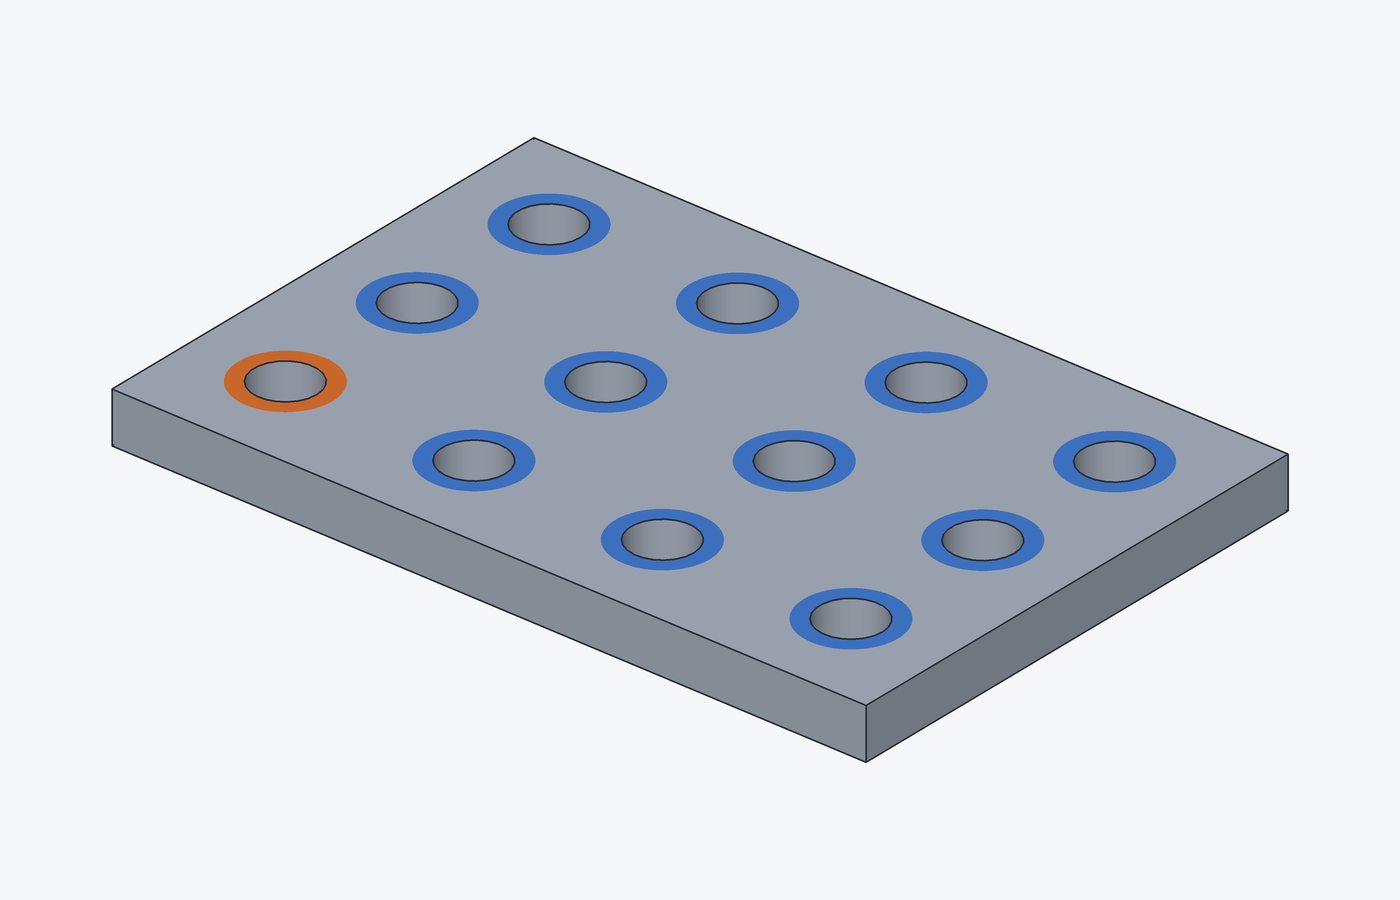
\includegraphics[width=\linewidth]{fig/rect_feature.png}
  \caption{Feature, rectangular: $4\times3$ holes (\code{LinearPattern}, two directions).}\end{subfigure}\hfill
\begin{subfigure}{0.49\linewidth}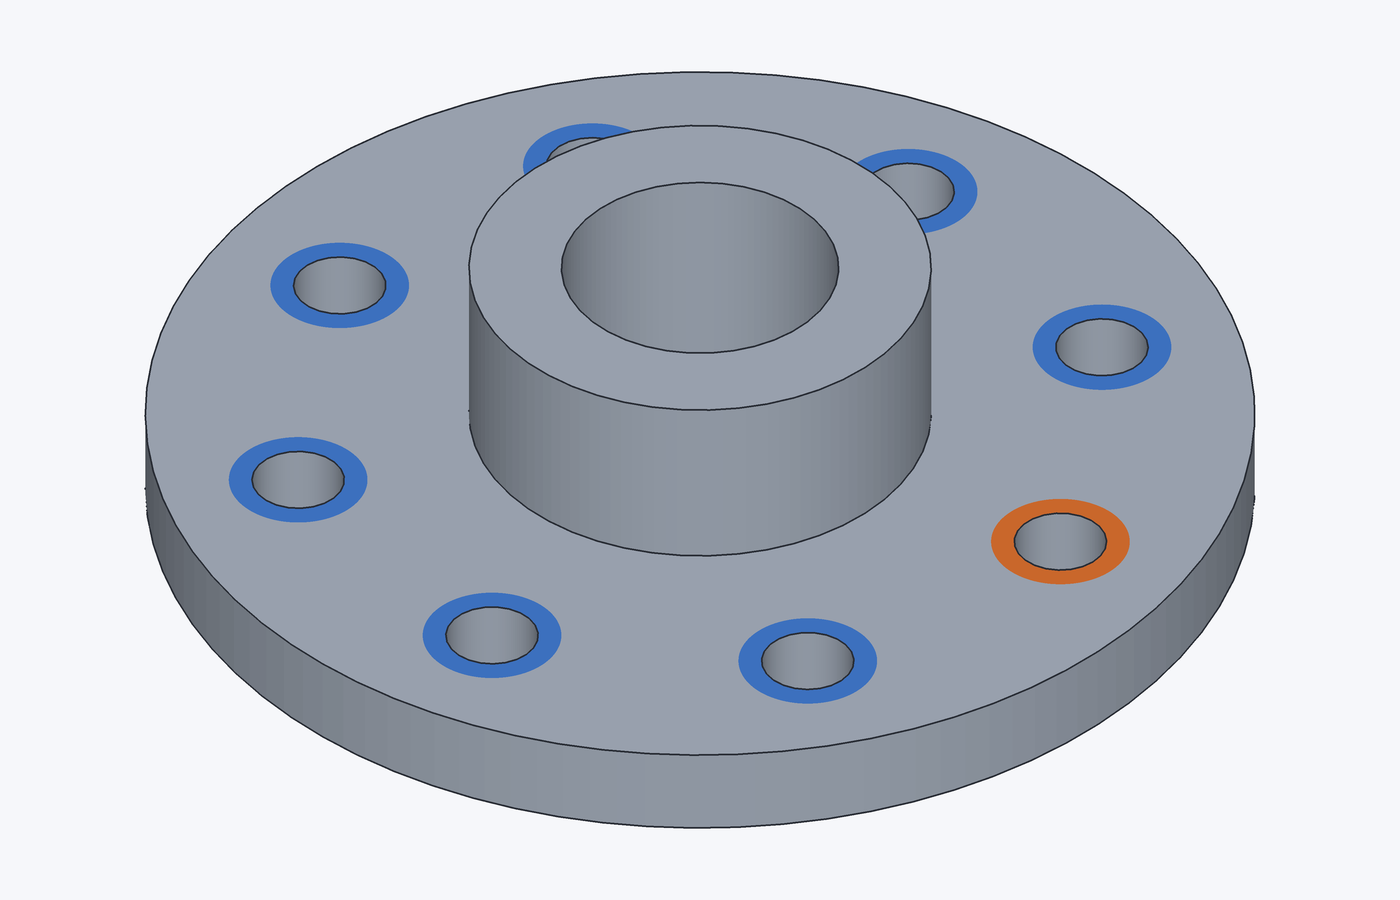
\includegraphics[width=\linewidth]{fig/circ_feature.png}
  \caption{Feature, circular: 8 bolt holes (\code{PolarPattern}, Full).}\end{subfigure}\\[4pt]
\begin{subfigure}{0.49\linewidth}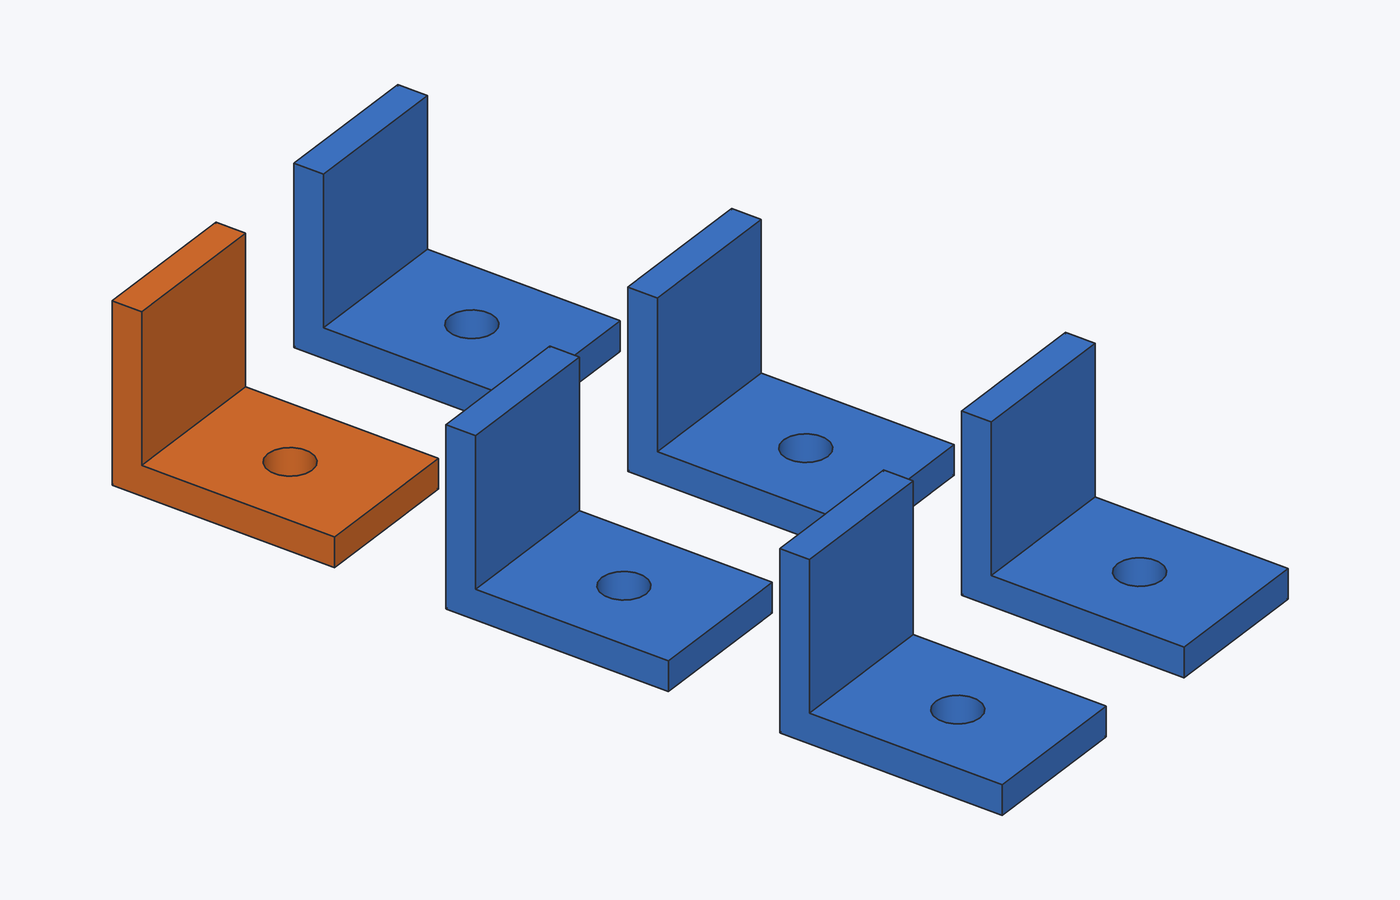
\includegraphics[width=\linewidth]{fig/body_pattern.png}
  \caption{Bodies, rectangular: $3\times2$ brackets (link array).}\end{subfigure}\hfill
\begin{subfigure}{0.49\linewidth}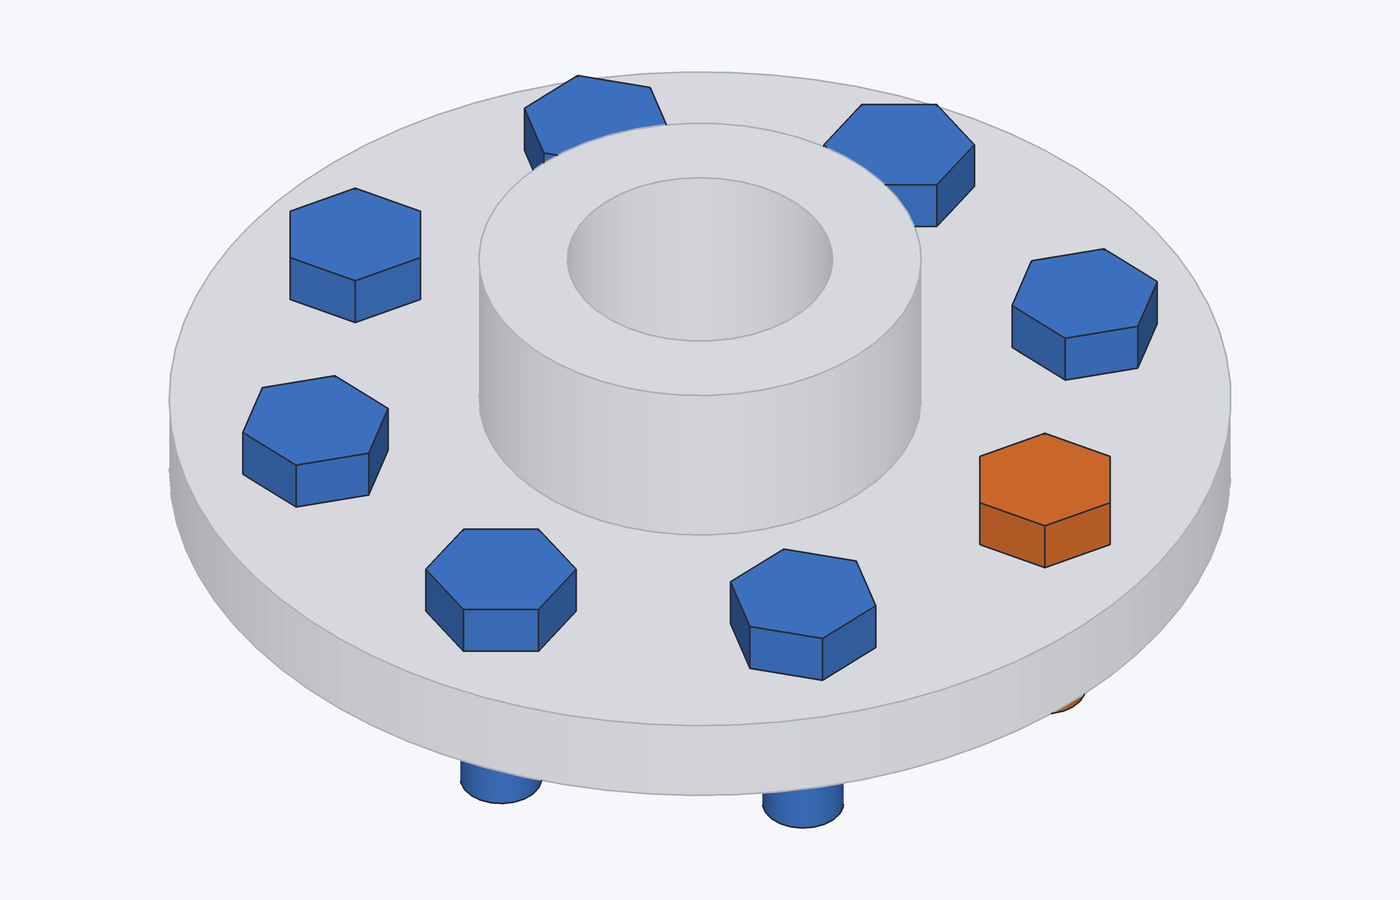
\includegraphics[width=\linewidth]{fig/component_pattern.png}
  \caption{Components, circular: 8 bolts around the flange axis.}\end{subfigure}
\caption{Pattern examples. Seed in \textcolor{bworange}{orange}, generated instances in
\textcolor{bwblue}{blue}. Panels (a) and (b) are real PartDesign features recomputed in headless FreeCAD
1.1.4 (panel (a) with the direction-2 workaround). Panel (c) was built with Draft's link array (6 elements
confirmed). Panel (d) uses the same transforms as the component command.}
\label{fig:examples}
\end{figure}

\subsubsection*{Theory}

\paragraph{Rigid motions.} An instance is the seed moved by a rigid motion $g\in SE(3)$,
\[
  g = \begin{pmatrix} R & \mathbf t\\ \mathbf 0^{\!\top} & 1\end{pmatrix},\qquad
  R\in SO(3),\ \mathbf t\in\mathbb R^3 .
\]
A pattern is a finite family $\{g_k\}_{k\in K}$ with $g_{\mathbf 0}=I$ (the seed). Features change one solid
with Booleans, $S\cup\bigcup_{k\neq 0} g_k(T)$ (additive) or $S\setminus\bigcup_{k\neq0} g_k(T)$
(subtractive), where $S$ is the support and $T$ the seed's tool shape. Bodies and components only produce
\emph{placements} $\{g_k P_0\}$, so no Boolean is evaluated.

\paragraph{Rectangular lattice.} With unit directions $\mathbf u_1,\mathbf u_2$ and per-gap spacings
$s^{(a)}_q$,
\[
  \mathbf t_{ij} = d_1(i)\,\mathbf u_1 + d_2(j)\,\mathbf u_2,\qquad
  d_a(m) = \operatorname{sgn}(m)\sum_{q=1}^{|m|} s^{(a)}_q .
\]
In \emph{Extent} mode $s_a = L_a/(n_a-1)$, and in \emph{Spacing} mode $L_a=(n_a-1)s_a$. These are
\code{calculateOffsetVector} and \code{calculateSteps} in \file{FeatureLinearPattern.cpp}. The index sets are
$I_a^{\text{one}}=\{0,\dots,n_a-1\}$ and $I_a^{\text{sym}}=\{-\lfloor\tfrac{n_a-1}{2}\rfloor,\dots,\lceil\tfrac{n_a-1}{2}\rceil\}$,
and $K=(I_1\times I_2)\setminus K_{\text{supp}}$. Translations commute, so the order of the two directions is
irrelevant. Instances are distinct iff every $s^{(a)}_q\neq0$ and $\mathbf u_1\nparallel\mathbf u_2$. The
bug below breaks the first condition.

\paragraph{Circular pattern.} About an axis through $\mathbf c$ with direction $\mathbf a$, Rodrigues'
formula gives
$R(\mathbf a,\theta) = I + \sin\theta\,[\mathbf a]_\times + (1-\cos\theta)\,[\mathbf a]_\times^2$ and
$g_k:\mathbf p\mapsto\mathbf c+R(\mathbf a,\theta_k)(\mathbf p-\mathbf c)$. The schedule is
$\theta_k = 2\pi k/n$ for \emph{Full} (dividing by $n$, since $2\pi\equiv0$), and
$\theta_k=\Theta k/(n-1)$ for \emph{Angle} ($k\in I^{\text{one}}$) and \emph{Symmetric}
($k\in I^{\text{sym}}$). Rotations about different axes do not commute, so nested patterns use a fixed
order, $g=g^{\text{outer}}_k\,g^{\text{inner}}_{ij}$.

\paragraph{Placements.} Pattern transforms are defined in world coordinates, so instance placements are
the left product $P_k=g_kP_0$. The right product $P_0g_k$ would pattern in the seed's local frame.

\paragraph{Linked vs.\ independent.} A link array stores the seed B-rep once plus $n$ placements,
$O(|B|+n)$ memory, and follows edits. Independent copies cost $O(n|B|)$. Verified headless:
\code{App::Link} with \code{ElementCount}$=8$ produced 8 \code{App::LinkElement}s and a compound of 8
solids. \code{setElementVisible("3", False)} dropped it to 7, which gives suppression for bodies and
components with no new code.

\paragraph{Compute modes.} Fusion's \emph{Identical} equals FreeCAD's \code{TransformMode = Features}
(the tool shape is copied). \emph{Adjust} re-evaluates each instance's terminations and needs a re-execute per
instance, so it is deferred (\S\ref{sec:questions}).

\begin{figure}[ht]
\centering
\begin{subfigure}{0.49\linewidth}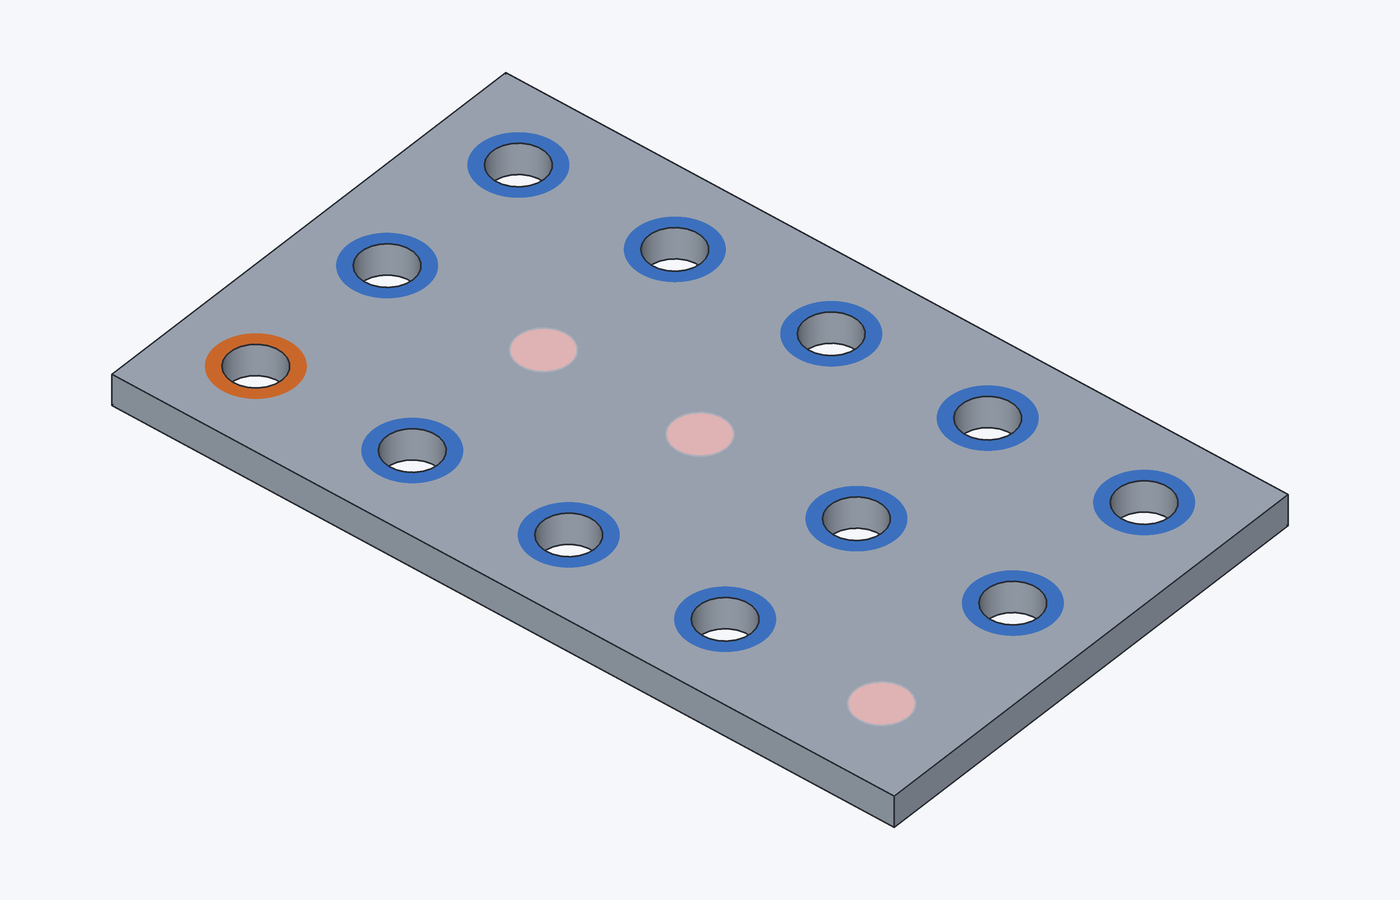
\includegraphics[width=\linewidth]{fig/suppression.png}
  \caption{Suppression: $K=(I_1\times I_2)\setminus K_{\text{supp}}$, $|K|=12$.}\end{subfigure}\hfill
\begin{subfigure}{0.49\linewidth}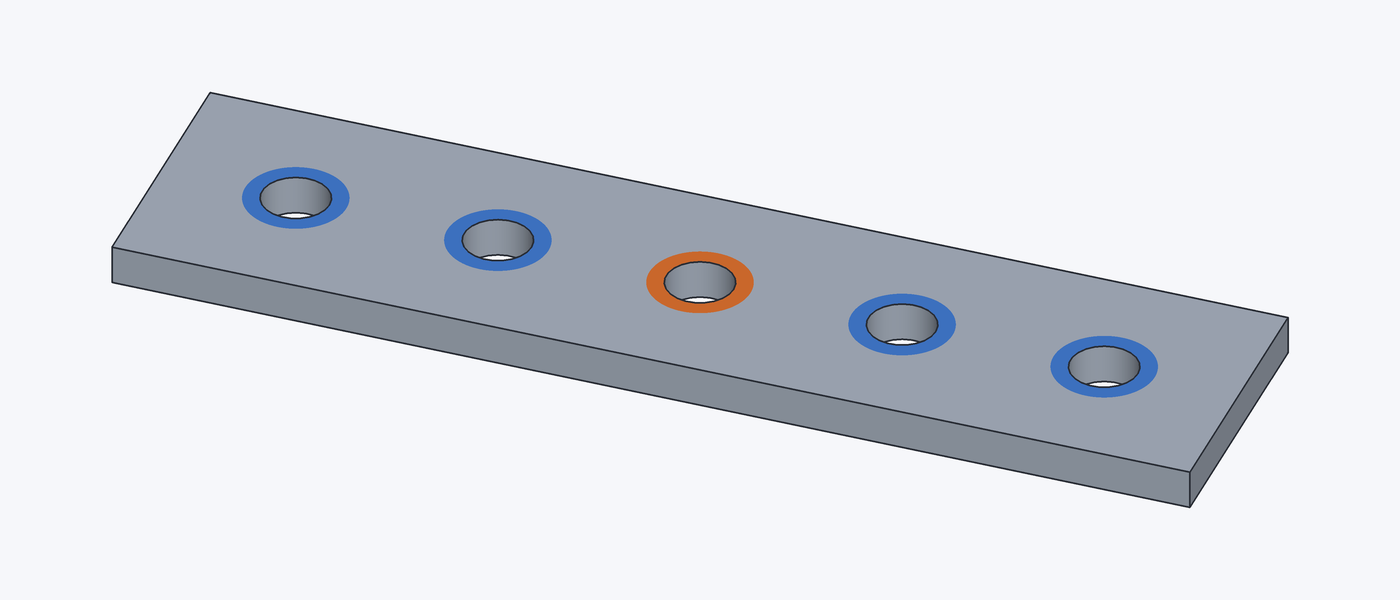
\includegraphics[width=\linewidth]{fig/symmetric.png}
  \caption{Symmetric direction, $n=5$: $I=\{-2,\dots,2\}$.}\end{subfigure}
\caption{The two new pattern options (target behaviour, not output of existing FreeCAD features).}
\label{fig:new}
\end{figure}

\paragraph{The direction-2 bug.}\label{sec:bug}
\begin{center}
\small
\begin{tabular}{@{}lccc@{}}
\toprule
Probe (headless FreeCAD 1.1.4) & rows asked & rows made & \code{Spacings2}\\
\midrule
Spacing 25\,mm, $n_2=3$ & 3 & 2 ($y=15,40$) & \code{[0.0, -1.0]}\\
Extent 50\,mm, $n_2=3$ & 3 & 3 & \code{[0.0, -1.0]}\\
Spacing 25\,mm, $n_2=5$ & 5 & 4 & \code{[0.0, -1.0, -1.0, -1.0]}\\
Direction 1, Spacing 30\,mm, $n_1=4$ & 4 & 4 & (\code{Spacings} correct)\\
\bottomrule
\end{tabular}
\end{center}
\begin{lstlisting}[language=C++]
ADD_PROPERTY_TYPE(Spacings,  ({-1.0}), "Direction 1", ...);  // ok
ADD_PROPERTY_TYPE(Spacings2, ({}),     "Direction 2", ...);  // {} -> setValue(double{}) -> [0.0]
\end{lstlisting}
The leading $0.0$ survives \code{updateSpacings}, so the first cumulative step is zero and a duplicate row
lands on the seed. Fixed on 19 Oct 2026: declared \code{(\{-1.0\})}, normalised in the constructor (as upstream main now
does), and a stored $0$ is mapped to $-1$ and written back, which repairs saved files. Three regression tests
(spacing, extent, old-file repair); all 171 PartDesign tests pass. Upstream main still declares
\code{(\{\})}; its constructor masks the bug for new objects but not for saved files, so the repair is worth
upstreaming (\eref{FND-06}).

\paragraph{Commands (built 19 Oct 2026, in GUI testing).} \code{BruceWorx\_RectangularPattern} and
\code{BruceWorx\_CircularPattern} (\file{bruceworx\_pattern.py}, \file{bruceworx\_pattern\_gui.py}) dispatch on
the selection. \emph{PartDesign features} go to PartDesign's own Linear/Polar Pattern. \emph{Bodies, Part
solids and assembly components} get an \code{App::Link} array whose parameters are dynamic properties in a
``BruceWorx Pattern'' group: rectangular (two directions, spacing or extent, symmetric) or circular (full,
angle, symmetric; axis from X/Y/Z, a straight edge, a circular edge's centre or a datum axis), suppression
per instance, and linked or independent copies. A task panel previews live, and Cancel removes everything
with or without document undo. Moving the seed re-places the pattern. In an assembly, the array's elements
count as components (\code{UtilsAssembly.isLinkGroup}; verified 6 components for a 6-up bolt pattern).
19 headless tests plus offscreen dialog smoke tests.

\paragraph{Upstream changes the feature path.} Upstream \code{main} (June--October 2026, PRs \#30417 and
\#32843) moved Linear/Polar Pattern logic into \code{Part::LinearPatternExtension} and friends and added
per-instance suppression (\code{SuppressedPositions}). Symmetric directions and suppression for
\emph{features} are therefore taken from upstream after the rebase (\eref{FND-03}), not written again on
1.1.4. Symmetric for features remains a candidate upstream contribution.

\begin{figure}[ht]
\centering
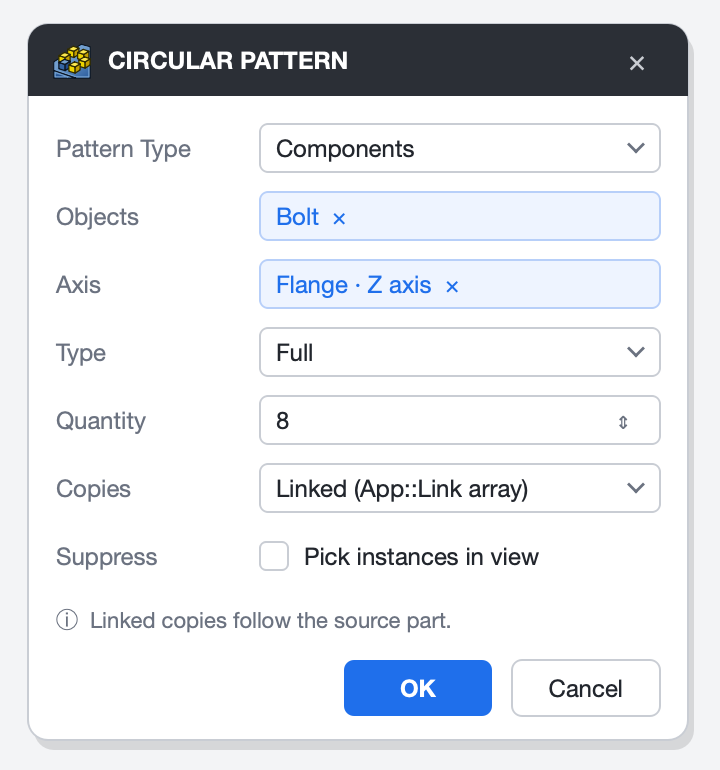
\includegraphics[width=0.36\linewidth]{fig/dialog_circ.png}
\caption{Circular Pattern dialog for components (working mock). \emph{Copies} shows for bodies and
components; \emph{Compute} only for features.}
\end{figure}

%----------------------------------------------------------------------
\subsection{BW-MOD-02 --- Parameters and top-down design}
%----------------------------------------------------------------------

\begin{epic}{MOD-02}{Parameters \& top-down design}{M1}{\stTodo}{(new)}
\begin{itemize}
  \item \textbf{Change Parameters} dialog (Fusion's name) listing every user parameter with its expression,
        value, unit and comment, drawn from \code{VarSet}s, Spreadsheet aliases and named feature
        dimensions, with search and favourites.
  \item \textbf{Skeleton} workflow: a master sketch or skeleton part drives layout, and parts consume it
        through \code{SubShapeBinder} across files. That fits the one-file-per-part model (\eref{ASM-01}).
  \item \textbf{Derive}: bring selected bodies, sketches or parameters from another file in as a linked,
        read-only reference, like SolidWorks' Insert Part or Fusion's Derive.
\end{itemize}
\emph{Acceptance:} changing a skeleton dimension updates three linked part files in one recompute.
\end{epic}

\paragraph{Theory: the recompute graph.} A document is a directed graph $G=(V,E)$ with an edge $u\to v$
when $v$ reads $u$ through a link or an expression. Recompute evaluates $V$ in a topological order of $G$,
in $O(|V|+|E|)$ time, and only for the \emph{touched} set's descendants. Top-down design adds edges
\emph{between documents}. The combined graph must stay acyclic. A part that binds geometry from an assembly
which contains that same part would close a cycle $p\to a\to p$. The tooling therefore refuses that
binding up front, rather than letting recompute fail. It allows a skeleton part referenced by both instead.

%----------------------------------------------------------------------
\subsection{BW-MOD-03 --- Configurations}
%----------------------------------------------------------------------

\begin{epic}{MOD-03}{Configurations}{M1}{\stTodo}{(new)}
One part or assembly file holds several variants (Fusion: Configurations; SolidWorks: configurations and
design tables). A \textbf{configuration table} object has rows for configurations and columns for parameters,
feature suppression states, custom properties (including the part number), and for assemblies, which
configuration each component uses. Activating a row writes the values and recomputes.
\emph{Acceptance:} Short, Standard and Long brackets come from one file
(Figure~\ref{fig:cfg}), and the BOM lists each configuration's own P/N.
\end{epic}

\begin{figure}[ht]
\centering
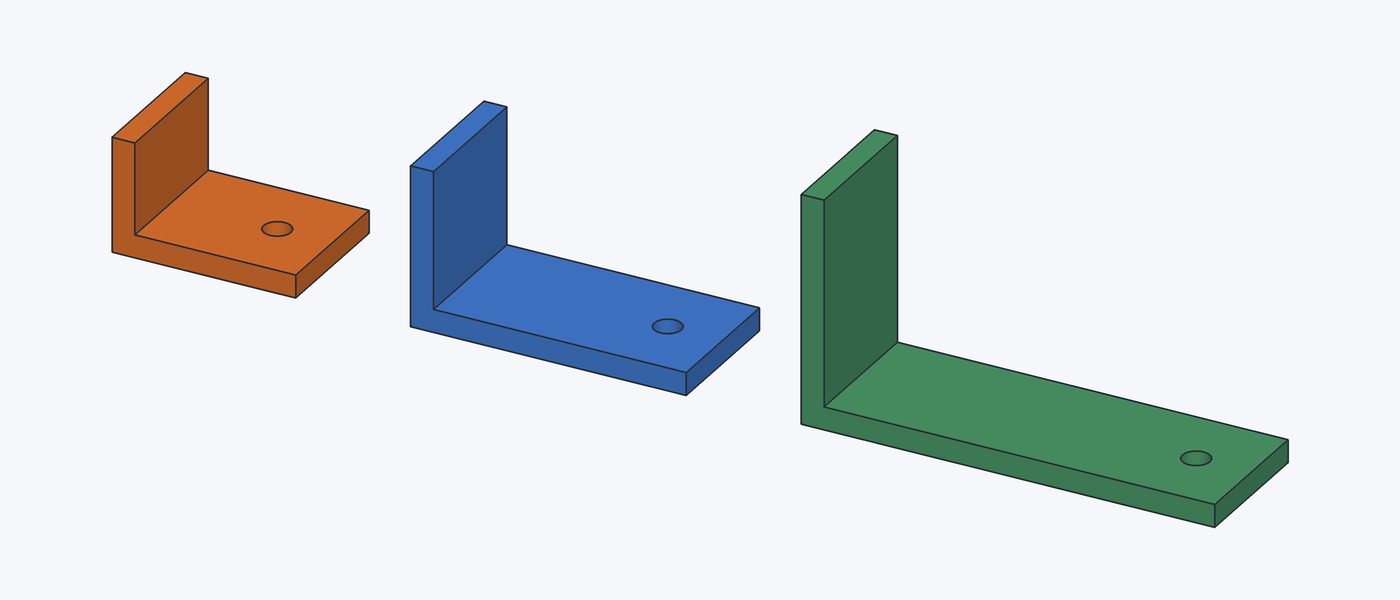
\includegraphics[width=0.85\linewidth]{fig/cfg_bracket.png}
\caption{Three configurations of one PartDesign body. A \code{VarSet} drives \code{Length}, \code{Height}
and the hole position by expression, and recomputing with three value sets gives volumes of
8\,858.6, 13\,358.6 and 20\,108.6\,mm$^3$. This is the mechanism the configuration table automates.
Built by \file{scripts/render\_roadmap.py}.}
\label{fig:cfg}
\end{figure}

\paragraph{Theory.} Let $\mathbf p\in\mathcal P$ be the parameter vector and $\mathbf s\in\{0,1\}^{F}$
the suppression state of $F$ features. A configuration is $c_j=(\mathbf p_j,\mathbf s_j,\pi_j)$, where
$\pi_j$ holds its properties (P/N, description, material). The model is a function $M(\mathbf p,\mathbf s)$
evaluated by recompute. Configurations change \emph{inputs only}, never topology of the feature graph, so
one history serves all rows. Two consequences follow:
\begin{enumerate}
  \item Each configuration is a distinct item for manufacturing, so it carries its \textbf{own P/N}. The BOM
        resolves a component to $(\text{file},c_j)$, not just to a file.
  \item Topological naming must survive a row switch. A fillet on an edge that exists only when a feature is
        unsuppressed has to be suppressed in the rows where that edge is missing. Per-row validation runs
        every configuration in CI and reports which features fail in which rows.
\end{enumerate}
Storage: a \code{BruceWorx::ConfigurationTable} object (FeaturePython) in the part file. It can import and
export CSV, so variants can be edited in a spreadsheet, as with a SolidWorks design table.

%----------------------------------------------------------------------
\subsection{BW-MOD-04 --- Direct edit on imported geometry}
%----------------------------------------------------------------------

\begin{epic}{MOD-04}{Direct edit on imported geometry}{M1}{\stTodo}{FCB-P2-15}
Edit ``dumb'' solids from STEP (Fusion exports, vendor parts) without a feature history:
\textbf{delete face} (exists: \code{Part\_Defeaturing}), \textbf{press-pull / offset face},
\textbf{move face} (translate or rotate), \textbf{replace face} (with a surface), plus \textbf{feature
recognition} that turns cylindrical cut faces into editable holes. Each edit is a parametric feature on top
of the imported shape, so it appears in the timeline.
\emph{Acceptance:} the Fusion STEP of \code{LE-01001} has a hole moved and a face offset, and stays valid.
\end{epic}

\begin{figure}[ht]
\centering
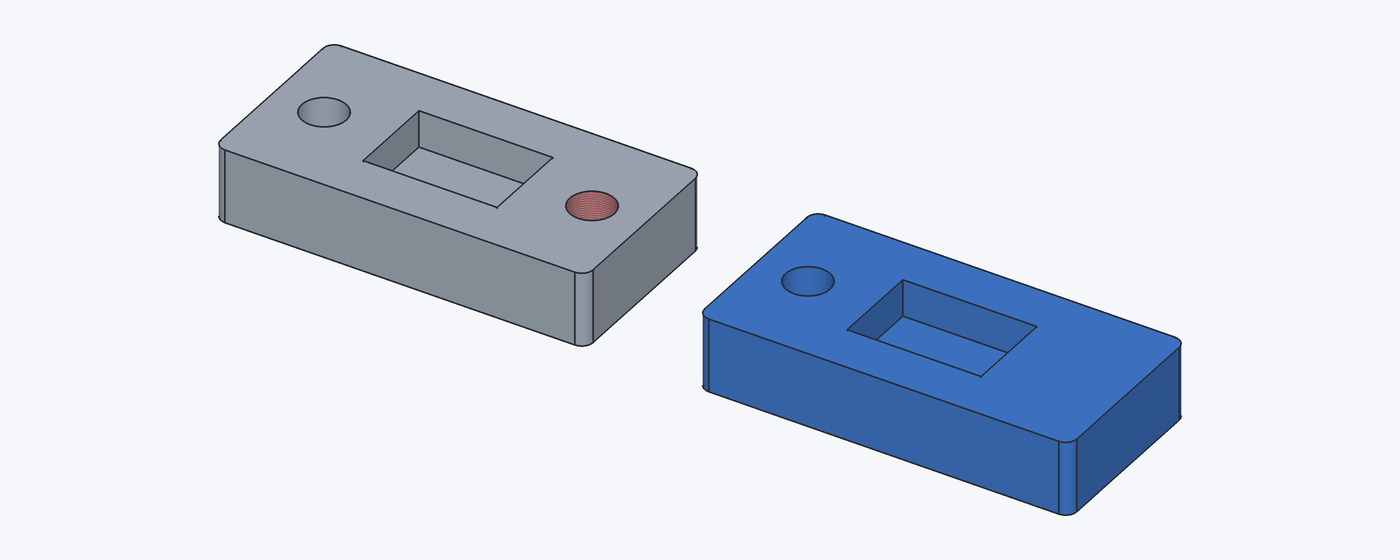
\includegraphics[width=0.85\linewidth]{fig/direct_edit.png}
\caption{Direct edit available today. A filleted block is exported to STEP and re-imported as a dumb solid
(17 faces). The right-hand hole's faces (red) are removed with \code{Shape.defeaturing} in headless
FreeCAD, giving 16 faces and a valid solid (blue). Press-pull, move and replace face build on the same kind of
local operation.}
\label{fig:direct}
\end{figure}

\paragraph{Theory: local face offset.} Press-pull replaces a face $F$ on surface $S(u,v)$ with its offset
$S_d(u,v)=S(u,v)+d\,\mathbf n(u,v)$, then re-intersects $S_d$ with the surfaces of the faces adjacent to $F$
to rebuild the edges, and extends or trims those neighbours. That is OCCT's
\code{BRepOffsetAPI\_MakeOffsetShape} in local mode, or \code{BRepFeat} for planar faces. Validity
conditions:
\begin{itemize}
  \item $|d|$ must stay below the minimum radius of curvature of $S$ where $d$ points to the concave side,
        or the offset self-intersects;
  \item each neighbour must still intersect $S_d$. A neighbour that ``runs out'' (a blend narrower than $d$)
        is removed first, which is how Fusion handles fillets that disappear when a face is pushed.
\end{itemize}
\textbf{Feature recognition:} cylindrical faces sharing an axis, with a closed boundary on a planar face,
become a hole candidate $(\mathbf c,\mathbf a,r,\text{depth})$. Counterbores are coaxial pairs with
$r_2>r_1$. The recognised hole is replaced by a real \code{Hole} feature, which also feeds drawing callouts
(\eref{DRW-04}).

%----------------------------------------------------------------------
\subsection{BW-MOD-05 --- Threads, holes and hardware}
%----------------------------------------------------------------------

\begin{epic}{MOD-05}{Threads, holes \& hardware library}{M1}{\stTodo}{FCB-P2-09/10, (new)}
\begin{itemize}
  \item \textbf{Cosmetic thread} object attached to a cylindrical face, storing standard, size, pitch,
        class, length, and handedness. It is shown in 3D as a texture/helix decoration, exported in STEP
        AP242 PMI where supported, and read by TechDraw for callouts.
  \item \textbf{Hole presets} (Hole Wizard parity): clearance (close/normal/loose), tapped, counterbore
        and countersink per fastener, plus \textbf{heat-set insert} holes by insert part number, the common
        case for FDM parts.
  \item \textbf{Fastener library}: evaluate the FreeCAD Fasteners add-on (licence and maintenance
        \verify) against a BruceWorx library built on the COTS schema (\eref{ROB-01}).
\end{itemize}
\emph{Acceptance:} an M3 tapped hole and an M3 heat-set hole both produce correct callouts on the drawing.
\end{epic}

\paragraph{Theory: thread geometry.} For ISO metric threads of nominal diameter $d$ and pitch $P$, the
fundamental triangle height is $H=\tfrac{\sqrt3}{2}P$. The basic internal minor diameter is
$D_1=d-2\cdot\tfrac{5}{8}H = d-1.0825\,P$, and the external minor diameter is $d_3=d-1.2269\,P$. Tap drill
$\approx d-P$ (M3$\times$0.5 $\rightarrow$ 2.5\,mm). A cosmetic thread stores $(d,P,\text{class},L)$ and draws
the minor/major diameter circle in views. Modelled threads (\code{ModelThread}) are kept for 3D printing,
where the printed geometry is the thread.

%----------------------------------------------------------------------
\subsection{BW-MOD-06 --- Sheet metal}
%----------------------------------------------------------------------

\begin{epic}{MOD-06}{Sheet metal}{M3}{\stTodo}{(new, from the UI plan)}
Bundle the SheetMetal add-on (decided; LGPL-2.1-or-later since v0.4.00) and add per-material, per-thickness
\textbf{rules} (bend radius, K-factor, relief) as a library, like Fusion's sheet-metal rules. Flats and
DXF are covered in \eref{MFG-03}, and the drawing in \eref{DRW-07}.
\emph{Acceptance:} the bracket in Figure~\ref{fig:sheet} unfolds to the length given by the bend-allowance
formula within 0.01\,mm.
\end{epic}

\begin{figure}[ht]
\centering
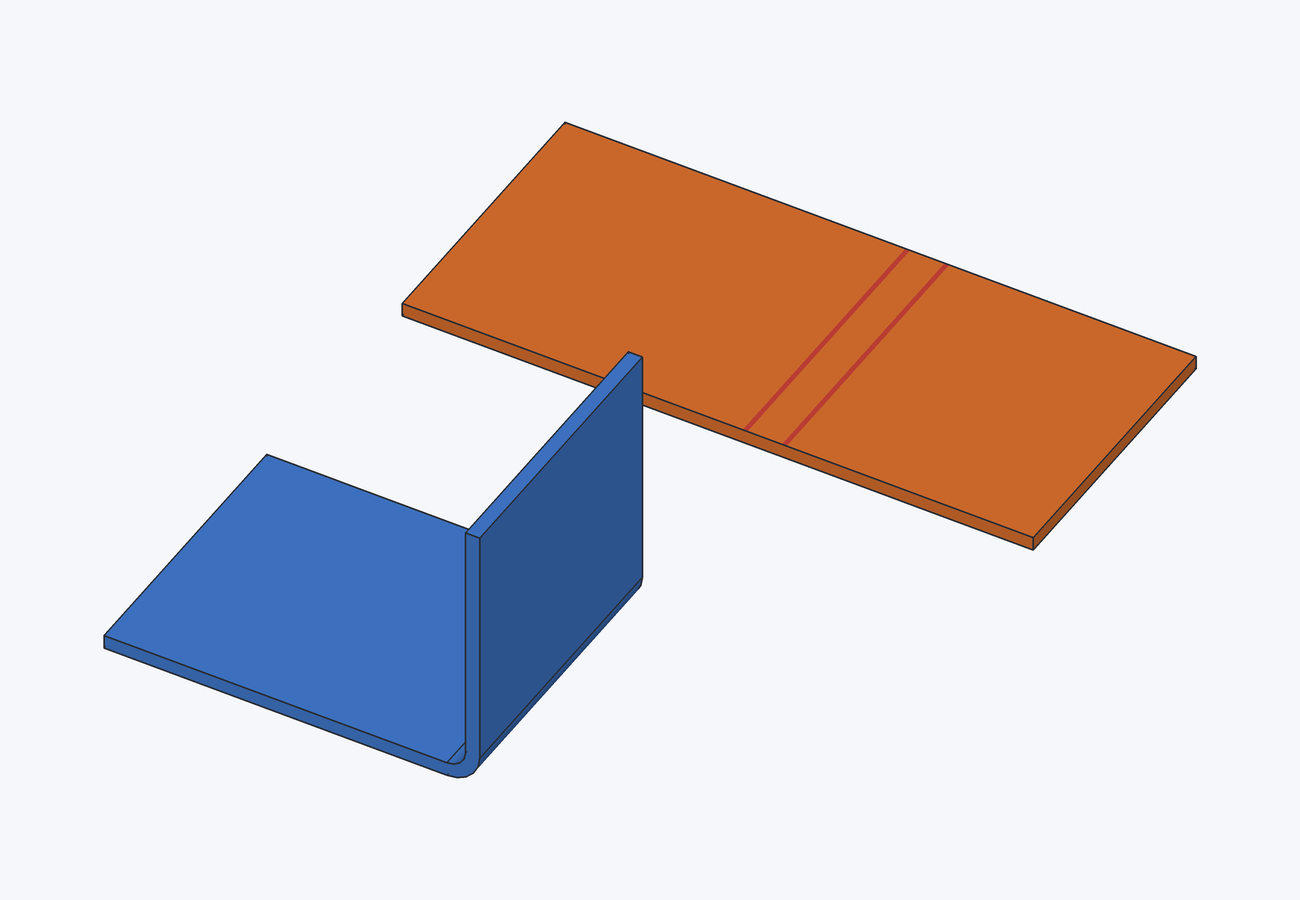
\includegraphics[width=0.62\linewidth]{fig/sheet_flat.png}
\caption{90$^\circ$ bracket (blue): $T=1.5$, $R_i=2$, outside flanges 40 and 30\,mm, depth 30\,mm, built as one
valid solid (volume 3\,029.4\,mm$^3$, matching the analytic value). Its flat (orange) is 67.178\,mm long, with
the bend zone between the red lines ($BA=4.178$\,mm at $K=0.44$).}
\label{fig:sheet}
\end{figure}

\paragraph{Theory: bend allowance.} During bending the neutral fibre sits at $R_i+KT$ from the bend axis,
with $0<K<0.5$ depending on material and process. Its arc length is the bend allowance
\[
  BA=\theta\,(R_i+K\,T),\qquad
  L_{\text{flat}} = \sum_i \ell_i + \sum_j BA_j ,
\]
where $\ell_i$ are the straight lengths between bend tangent lines. For the bracket,
$\ell_1=40-(2+1.5)=36.5$, $\ell_2=30-3.5=26.5$, and $BA=\tfrac{\pi}{2}(2+0.44\cdot1.5)=4.178$, so
$L_{\text{flat}}=67.178$\,mm. $K$ comes from the rules library per material, thickness and tooling. That is
why the rules table matters more than the unfold algorithm.

%----------------------------------------------------------------------
\subsection{BW-MOD-07 --- Frames and weldments}
%----------------------------------------------------------------------

\begin{epic}{MOD-07}{Frames \& weldments}{M3}{\stTodo}{(new)}
Structural members swept along 3D-sketch edges from a \textbf{profile library}: 2020/2040 aluminium
extrusion, square and round tube, angle, flat bar. Each joint gets an \textbf{end treatment} (mitre, butt
one or the other, cope), and \textbf{trim/extend} works against other members. The \textbf{cut list} groups
identical members and gives stock length, angles and quantity. Each member is a body with a cut-list item, not
a separate part file.
\emph{Acceptance:} the frame in Figure~\ref{fig:frame} produces the cut list below.
\end{epic}

\begin{figure}[ht]
\centering
\begin{minipage}{0.48\linewidth}
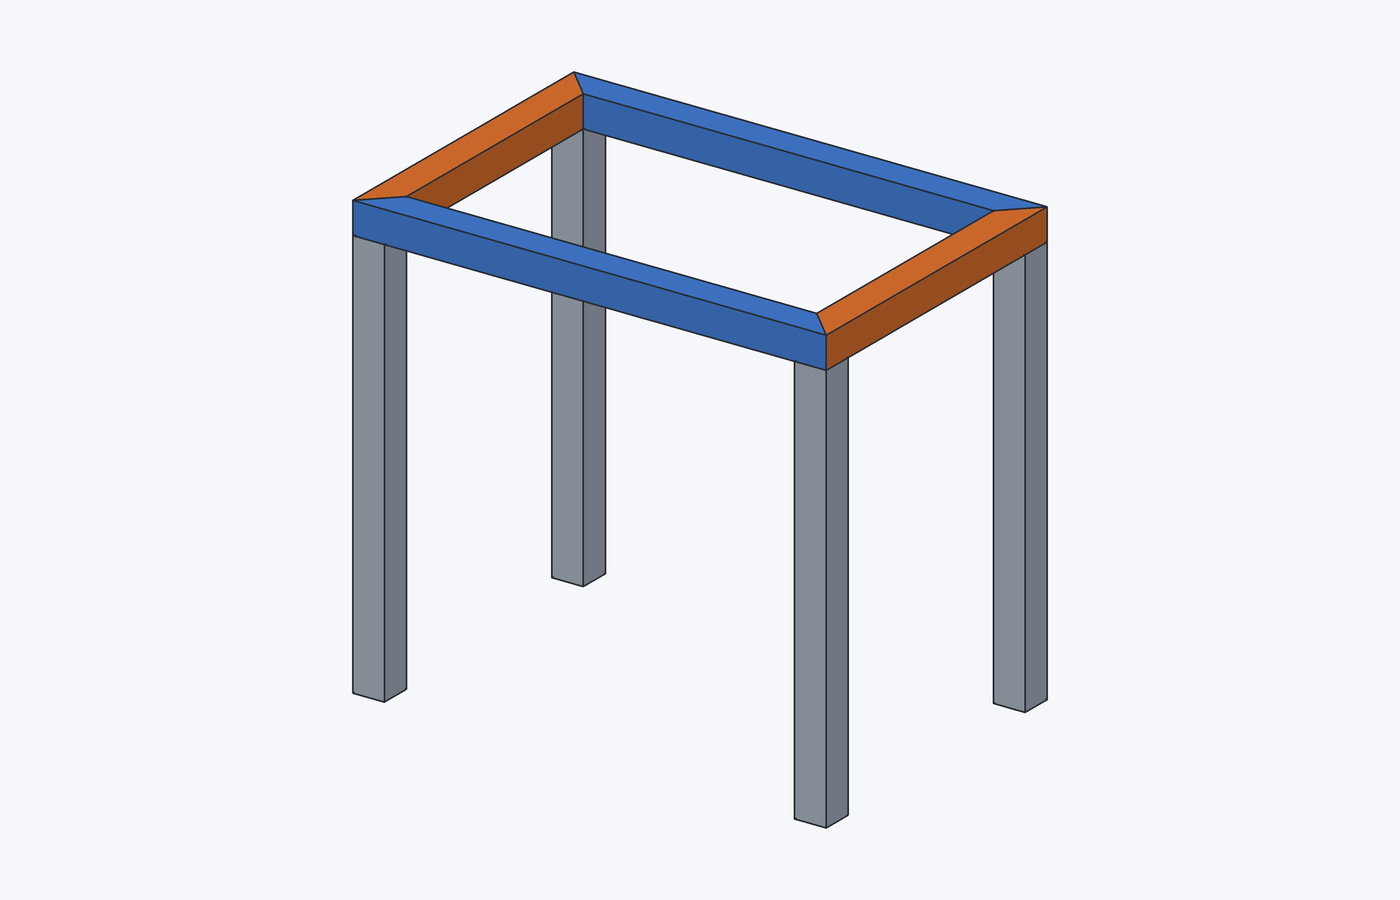
\includegraphics[width=\linewidth]{fig/frame_weldment.png}
\end{minipage}\hfill
\begin{minipage}{0.48\linewidth}
\small
\begin{tabular}{@{}lccc@{}}
\toprule
Member & Qty & Length (outer/inner) & Ends\\
\midrule
Top, long & 2 & 300 / 260 & 45/45\\
Top, short & 2 & 200 / 160 & 45/45\\
Leg & 4 & 260 & 0/0\\
\bottomrule
\end{tabular}\\[4pt]
{\footnotesize 20$\times$20 profile. Generated by \file{render\_roadmap.py}; the fused frame is a valid solid.}
\end{minipage}
\caption{Mitred top frame on butt-jointed legs, and its cut list.}
\label{fig:frame}
\end{figure}

\paragraph{Theory: mitre plane.} Two members meet at corner $\mathbf c$ with unit directions
$\hat{\mathbf d}_1$ (incoming) and $\hat{\mathbf d}_2$ (outgoing). The mitre plane passes through $\mathbf c$
with normal
\[
  \mathbf n=\frac{\hat{\mathbf d}_1+\hat{\mathbf d}_2}{\lVert\hat{\mathbf d}_1+\hat{\mathbf d}_2\rVert},
\]
which bisects the turn. Each member is cut by the half-space on its own side. With turn angle
$\alpha=\arccos(\hat{\mathbf d}_1\!\cdot\hat{\mathbf d}_2)$, the cut is $\alpha/2$ from square, so a
90$^\circ$ corner gives 45$^\circ$. For profile width $w$, the outer edge is longer than the centre line by
$\tfrac{w}{2}\tan\tfrac{\alpha}{2}$ at each mitred end, and the inner edge shorter by the same amount. With
$w=20$ the centre lines are 280 and 180\,mm, which gives the 300/260 and 200/160 pairs above.

%----------------------------------------------------------------------
\subsection{BW-MOD-08 --- Surfacing parity}
%----------------------------------------------------------------------

\begin{epic}{MOD-08}{Surfacing parity}{M5}{\stTodo}{(new)}
Fill the gaps next to the Surface workbench: trim and untrim by curve or surface, patch (n-sided, with
continuity per edge), extend, stitch into a solid, replace face, and thicken. Add \textbf{continuity
analysis} (zebra stripes, curvature comb, deviation map), which is how surfacing is checked in Fusion and
SolidWorks.
\emph{Acceptance:} a surface benchmark set rebuilt to the stated G1/G2 continuity, and thickened into a
valid solid.
\end{epic}

\paragraph{Theory: continuity.} Two surfaces meeting along a curve are $G^0$ if positions match, $G^1$ if
tangent planes match ($\mathbf n_1=\pm\mathbf n_2$ along the curve), and $G^2$ if normal curvatures match in
every direction. Zebra stripes are reflection lines of a striped environment. A stripe stays continuous
across a $G^1$ joint, and stays continuous \emph{and} smooth across $G^2$. That makes them a fast visual test
of the next-higher order. The tolerances checked are angular ($\le0.1^\circ$ for $G^1$) and relative curvature
($\le5\%$ for $G^2$).

%----------------------------------------------------------------------
\subsection{BW-MOD-09 --- Freeform (subdivision / T-spline-like)}
%----------------------------------------------------------------------

\begin{epic}{MOD-09}{Freeform}{M5}{\stTodo}{(new)}
A \textbf{Form body} like Fusion's Form workspace: start from a primitive cage, push and pull faces, edges and
vertices, extrude, crease, and mirror. The result converts to a B-spline B-rep solid that the rest of FreeCAD
can use. T-splines are proprietary, so the open path is \textbf{Catmull--Clark subdivision}, for example via
OpenSubdiv (Apache-2.0) \verify, with conversion to bicubic patches.
\emph{Acceptance:} a drone canopy modelled as a cage and exported as a valid STEP solid.
\end{epic}

\paragraph{Theory.} One Catmull--Clark step creates a face point $\mathbf f$ (the face centroid) and an edge
point $\mathbf e=\tfrac14(\mathbf v_1+\mathbf v_2+\mathbf f_1+\mathbf f_2)$, and moves each vertex of
valence $n$ to
\[
  \mathbf v'=\frac{\mathbf F+2\mathbf R+(n-3)\mathbf v}{n},
\]
with $\mathbf F$ the mean of adjacent face points and $\mathbf R$ the mean of adjacent edge midpoints. On
regular regions (quads, valence 4) the limit surface \emph{is} a uniform bicubic B-spline. Those patches
convert exactly to \code{Geom\_BSplineSurface}. Around extraordinary vertices ($n\neq4$) the limit surface
is not a finite B-spline, so conversion uses $G^1$ approximating patches (Gregory-type) within a tolerance,
and that tolerance is reported. Creases set sharp rules on tagged edges.

%----------------------------------------------------------------------
\subsection{BW-MOD-10 --- Mesh to solid}
%----------------------------------------------------------------------

\begin{epic}{MOD-10}{Mesh to solid}{M5}{\stTodo}{(new)}
A pipeline from STL, 3MF or scan to an editable solid: \textbf{repair} (holes, non-manifold edges, flipped
normals), \textbf{segment} into regions, \textbf{fit} planes, cylinders, cones and spheres, then
\textbf{rebuild} as intersecting analytic faces, or as features where they are recognised. A faceted solid
(\code{Part\_ShapeFromMesh}, which exists) remains the fallback.
\emph{Acceptance:} a scanned bracket becomes a solid with analytic faces within 0.1\,mm of the scan.
\end{epic}

\paragraph{Theory: RANSAC fitting.} To fit a primitive needing $s$ points (3 for a plane) to a region
where a fraction $w$ of points are inliers, the probability that $k$ random samples all fail is
$(1-w^s)^k$. Success with probability $p$ therefore needs $k=\lceil\log(1-p)/\log(1-w^s)\rceil$ samples.
For a plane with $w=0.5$ and $p=0.99$, that is $k=35$. Regions are grown from the best model, removed, and
the search repeats. Deviation is reported as the RMS and maximum point-to-surface distance.

%----------------------------------------------------------------------
\subsection{BW-MOD-11 --- Inspect tools}
%----------------------------------------------------------------------

\begin{epic}{MOD-11}{Inspect tools}{M1}{\stTodo}{FCB-P2R-07, (new)}
Measure (exists), \textbf{mass, centre of gravity and inertia} (extends \code{MeasureCOM}), \textbf{section
analysis} that stays in the model, \textbf{curvature/zebra} (shared with \eref{MOD-08}), \textbf{draft
analysis}, a \textbf{3D-print overhang map} against a build direction, and a \textbf{wall-thickness} map.
\emph{Acceptance:} mass and CG match a hand-calculated fixture; the overhang map flags the expected faces on a
printed part.
\end{epic}

\paragraph{Theory: overhang.} For build direction $\mathbf b$ (unit, up) and face normal $\mathbf n$, a
downward-facing region needs support when its angle from the horizontal is below the critical angle
$\theta_c$ (typically 45$^\circ$ for FDM), that is when
\[
  \mathbf n\cdot(-\mathbf b) > \cos\theta_c .
\]
The map colours each tessellation facet by $\mathbf n\cdot(-\mathbf b)$. Draft analysis is the same test
against a pull direction with $\theta_c$ equal to the draft angle. \textbf{Mass properties} are integrals
over the solid. For $N$ parts with masses $m_i$, centres $\mathbf c_i$ and inertia tensors $I_i$ about their
own centres, the assembly CG is $\bar{\mathbf c}=\sum m_i\mathbf c_i/\sum m_i$, and the parallel-axis theorem
gives $I=\sum_i\big(I_i+m_i(\lVert\mathbf r_i\rVert^2E-\mathbf r_i\mathbf r_i^{\!\top})\big)$ with
$\mathbf r_i=\mathbf c_i-\bar{\mathbf c}$ (see \eref{ROB-03}).

%----------------------------------------------------------------------
\subsection{BW-MOD-12 --- Sketcher parity audit}
%----------------------------------------------------------------------

\begin{epic}{MOD-12}{Sketcher parity audit}{M1}{\stTodo}{(new)}
Sketcher is mature, but full parity needs a checked list. Compare it against Fusion and SolidWorks sketch tools:
slots, conics, text, offset and project/include, sketch patterns, dimension-driven parameters, constraint
inference while drawing, and sketch-level mirror and fillet behaviours. Close the five most-used gaps.
\emph{Acceptance:} gap list approved; top five gaps closed.
\end{epic}

%======================================================================
\section{Track ASM --- Assembly}\label{sec:asm}
%======================================================================

FreeCAD 1.1's Assembly workbench already provides joints (Ondsel solver), grounding, exploded views
(\code{Assembly\_CreateView}), a BOM (\code{Assembly\_CreateBom}: Index, Name, File Name, Quantity, plus custom
columns) and kinematic simulation (\code{Assembly\_CreateSimulation}, new in 1.1). This track builds on
those. The file model comes first, because PDM, drawings and BOMs all depend on it.

\begin{epic}{ASM-01}{File model: one part per file}{M1}{\stTodo}{(new)}
SolidWorks-style, as decided: every part is its own \code{.FCStd} with its own P/N, and assemblies
reference parts through \code{App::Link} to external documents with \emph{relative} paths. Tooling:
\textbf{make external} (split the bodies of a multi-body design file into numbered part files and relink),
\textbf{pack and go} (copy an assembly with all its references), and a \textbf{broken-reference resolver}.
\emph{Acceptance:} \code{LE-02001} opens from a moved folder with no broken links.
\end{epic}

\paragraph{Theory: assemblies as a DAG.} Documents form a directed acyclic graph with edges assembly
$\rightarrow$ component and multiplicities $q$. A component \emph{occurrence} is a path
$a_0\to a_1\to\dots\to p$ from the top assembly. Its world placement is the product of the link placements
along the path, $P = P_{a_0a_1}P_{a_1a_2}\cdots P_{a_kp}$. Occurrences, not files, carry joints, colour
overrides and BOM item numbers. Making parts external changes nothing in occurrence space, only which
document owns the geometry. That is why the conversion can be automatic.

\begin{epic}{ASM-02}{Assembly gap audit}{M1}{\stDone}{FCB-P2A-01/02}
Audit current Assembly against a SolidWorks/Fusion checklist and against upstream main. \textbf{Approved
19 Oct 2026 (\S\ref{sec:asm-audit})}; it re-scopes \eref{ASM-03}--\eref{ASM-10}. Three behaviours still need the
screen and are in the test checklist.
\end{epic}

%======================================================================
\subsection{BW-ASM-02 --- Assembly gap audit (approved, 19 Oct 2026)}\label{sec:asm-audit}
%======================================================================

\textbf{Method.} The Assembly workbench in this repository (FreeCAD 1.1.4) was read command by command
(\file{src/Mod/Assembly}), and compared with a SolidWorks/Fusion checklist and with the 97 upstream commits
to \file{src/Mod/Assembly} since the 1.1 release (24 Mar -- 10 Oct 2026, GitHub API). The ``upstream'' column
is what the rebase to main (\eref{FND-03}) brings without any BruceWorx work. Items marked \verify{} need the
GUI and are in the next test session. \textbf{Gate:} the mechanical reviewer approves this list; it then
re-scopes \eref{ASM-03}--\eref{ASM-10}.

\begin{center}
\scriptsize
\setlength{\tabcolsep}{3pt}
\renewcommand{\code}[1]{\texttt{#1}}
\begin{longtable}{@{}>{\raggedright\arraybackslash}p{2.9cm}cc >{\raggedright\arraybackslash}p{4.6cm} >{\raggedright\arraybackslash}p{3.0cm} >{\raggedright\arraybackslash}p{2.3cm}@{}}
\toprule
Capability & SW & Fusion & FreeCAD 1.1.4 (this build) & Upstream main since 1.1 & Gap $\rightarrow$ epic\\
\midrule\endhead
\bottomrule\endfoot
\multicolumn{6}{@{}l}{\textbf{Joints}}\\
Fixed / rigid & \pfull & \pfull & \pfull{} Fixed & --- & ---\\
Revolute, slider, cylindrical, ball & \pfull & \pfull & \pfull{} all four & joint rotate button & ---\\
Planar & \pfull & \pfull & \phalf{} via Distance on two planes (solver \code{ASMTPlanarJoint}) & --- & UX: name it (ASM-03)\\
Tangent / cam & \pfull & \phalf & \phalf{} Distance 0 plane--cylinder = tangent; no cam & --- & cam: later\\
Pin-slot & \pnone & \pfull & \pnone & --- & ASM-03\\
Gear, rack-pinion, screw, belt & \pfull & \phalf & \pfull{} Gears, RackPinion, Screw, Belt & coaxial gear joint; rack-pinion fix & ---\\
Parallel, perpendicular, angle, distance & \pfull & \phalf & \pfull & --- & ---\\
Width / symmetric / path / slot mates & \pfull & \pnone & \pnone & --- & later (not in Fusion)\\
Quick joint (type inferred from picks; SW smart mates) & \pfull & \pfull & \pnone{} one command per type & ``put unconnected part second'' & ASM-03\\
Joint limits & \pfull & \pfull & \phalf{} Length/Angle min--max passed to solver (\code{ASMTTranslationLimit}, \code{ASMTRotationLimit}); honoured while dragging (verified headless); not by a plain solve. Zero from datums: built, section~\ref{sec:joints} & --- & ASM-03\\
As-built joints (no move) & \phalf & \pfull & \pfull{} \emph{Keep parts where they are} (built 19 Oct) & --- & ASM-03\\
Rigid groups & \pfull & \pfull & \pnone & \textbf{RigidGroup (\#29605)} & rebase\\
Edit joint from context menu & \pfull & \pfull & \phalf{} double-click & \textbf{``Edit joint'' entry} & rebase\\
\midrule
\multicolumn{6}{@{}l}{\textbf{Structure}}\\
Insert existing part & \pfull & \pfull & \pfull{} \code{Assembly\_InsertLink} & label fix & ---\\
New part in context & \pfull & \pfull & \pfull{} \code{Assembly\_InsertNewPart} creates \emph{and saves a separate document} --- matches one-file-per-part & joint creation fix & ASM-01 builds on it\\
Sub-assemblies, rigid vs flexible & \pfull & \pfull & \pfull{} \code{AssemblyLink.Rigid} & parent refresh; rigid-change fix & ASM-05 shrinks to verification\\
Grounding & \pfull & \pfull & \pfull & \textbf{grounded parts unmovable} & rebase\\
Component patterns & \pfull & \pfull & \pfull{} BruceWorx link arrays (MOD-01, today) & \textbf{generated arrays + suppressed elements} & align on rebase\\
Mirror components & \pfull & \pfull & \pnone & --- & new, small (ASM-03)\\
Position snapshots / configurations & \pfull & \pfull & \pnone & \textbf{snapshots (\#25384)} & rebase\\
\midrule
\multicolumn{6}{@{}l}{\textbf{Motion and checks}}\\
Free drag with solver & \pfull & \pfull & \pfull{} \code{preDrag}/\code{doDragStep} & island drag (\#30998); transformed-assembly fixes & rebase\\
Kinematic simulation / drive joints & \pfull & \pfull & \pfull{} \code{Assembly\_CreateSimulation} (Angular/Linear motions, formulas) & formula fixes; \textbf{video export (PyAV)} & ROB-05\\
Dynamic motion (gravity, forces, contact) & \pfull & \phalf & \pnone & --- & ASM-10\\
Collision detection during drag (Fusion contact sets) & \pfull & \pfull & \pnone & --- & ASM-06 (+ later)\\
Interference / clearance check & \pfull & \pfull & \pnone{} nothing in \file{src/Mod/Assembly} & --- & ASM-06\\
Degrees of freedom readout & \pfull & \phalf & \phalf & DoF fix with bundled fixed joints & ---\\
\midrule
\multicolumn{6}{@{}l}{\textbf{Documentation output}}\\
Exploded views & \pfull & \pfull & \pfull{} \code{Assembly\_CreateView} & \textbf{move controls (\#30955)} & rebase + ASM-04 presets\\
BOM & \pfull & \pfull & \phalf{} Index, Name, File Name, Quantity automatic; \textbf{custom columns read same-named properties of each part} (\code{BomObject.cpp:283}) & --- & ASM-04 = add P/N, Rev, Material, Mass \emph{properties} to parts (PDM-02)\\
Mass properties of assembly & \pfull & \pfull & \phalf{} \code{MeasureCOM} & --- & MOD-11, ROB-03\\
\midrule
\multicolumn{6}{@{}l}{\textbf{Scale}}\\
Large-assembly / lightweight mode & \pfull & \phalf & \pnone & --- & ASM-08\\
In-context editing & \pfull & \pfull & \phalf{} cross-document \code{SubShapeBinder} & --- & ASM-07\\
Smart fasteners & \pfull & \phalf & \pnone & --- & ASM-09\\
\end{longtable}
\end{center}

\paragraph{What the audit changes.}
\begin{enumerate}
  \item \textbf{Rebase first, then build.} Six rows close by rebasing (rigid groups, snapshots, exploded-view
        controls, edit-joint menu, grounded locking, island drag), and upstream now handles generated arrays and
        suppressed link elements. \eref{FND-03} moves ahead of \eref{ASM-03}.
  \item \textbf{\eref{ASM-04} gets smaller.} The BOM already reads any property by column name, so P/N, Rev and
        Material columns need only the PDM properties on each part (\eref{PDM-02}). Only \emph{Mass} needs new
        code: a computed property kept current on recompute.
  \item \textbf{\eref{ASM-05} becomes verification.} Rigid/flexible sub-assemblies exist
        (\code{AssemblyLink.Rigid}); the epic checks them on \code{LE-02001} and fixes what breaks.
  \item \textbf{\eref{ASM-03} keeps:} quick joint with type inference, pin-slot, mirror components, explicit
        Planar naming, limits verified while dragging, as-built behaviour.
  \item \textbf{Still entirely missing:} interference/clearance (\eref{ASM-06}), dynamic motion
        (\eref{ASM-10}), lightweight mode (\eref{ASM-08}), smart fasteners (\eref{ASM-09}) --- unchanged.
\end{enumerate}

\paragraph{For the next GUI session} (steps 14--16 of section~\ref{sec:tonight}).
\begin{description}[leftmargin=0pt]
  \item[(a) Limits while dragging.] \emph{Dragging} is moving a part with the mouse in the 3D view after it is
        jointed; the solver keeps the joints as you pull. Fusion and SolidWorks stop the part at a joint's limit.
        FreeCAD passes the limits to the solver; whether a drag stops at them is what the step records.
  \item[(b) Joints on pattern instances.] Required (answer, 19 Oct): a joint on a generated bolt must survive
        a change of pattern count while that bolt still exists, and fail with a clear message when it goes.
  \item[(c) Fixed joint placement.] A joint is made by picking a face or edge on each part; the solver then moves
        one part so the two picks line up. ``Stays put'' asks whether a Fixed joint between two parts you have
        already placed keeps them exactly where they are (Fusion calls this an \emph{as-built} joint), or snaps
        the second part so the picks coincide. Both are useful; the step records which FreeCAD does today, and
        \eref{ASM-03} adds the other.
\end{description}

\paragraph{Answered later on 19 Oct.} (a) Drag stays free; limits only when set in the joint, measured from a
datum. (c) Joints keep moving one part to line up the picks; a checkbox keeps parts where they are. Both are built
(section~\ref{sec:joints}); steps 14 and 16 now test them on screen.

\paragraph{Decision (19 Oct).} Audit approved. Part properties must stay open to growth: they now come from a
layered schema instead of code (section~\ref{sec:partprops}).

%======================================================================
\subsection{Part properties that can grow (built 19 Oct 2026)}\label{sec:partprops}
%======================================================================

\textbf{Requirement.} ``Make it so we can expand properties of parts later.'' The properties every part carries
(P/N, revision, description, material, mass, finish, vendor\ldots) are therefore data, not code: a list in
JSON that is read in layers. Adding a property means adding one line to a layer file; FreeCAD, the BOM and the
vault pick it up without a new build.

\begin{center}
\small
\begin{tabularx}{\linewidth}{@{}lX@{}}
\toprule
Layer (read in this order) & Holds\\
\midrule
1. Built in: \file{addons/BruceWorx/config/part\_properties.json} & The nine BruceWorx properties below. Ships with
  the build; not edited by hand.\\
2. Company or vault: e.g.\ \file{<vault>/part\_properties.json} & What your company adds: supplier, lead time,
  RoHS, cost centre\ldots\\
3. User: \file{\textasciitilde/.config/bruceworx/part\_properties.json} & Personal additions while trying something
  out.\\
\bottomrule
\end{tabularx}
\end{center}

\begin{center}
\small
\begin{tabular}{@{}lllll@{}}
\toprule
Property & Type & BOM column & Comes from & Needed at\\
\midrule
\code{PartNumber} & text & \code{.PartNumber} & vault (read-only) & ---\\
\code{Revision} & text & \code{.Revision} & vault (read-only) & ---\\
\code{Description} & text & \code{.Description} & you & submit\\
\code{ItemType} & choice & --- & you (part, assy, COTS, dwg) & ---\\
\code{MaterialName} & text & \code{.MaterialName} & computed: bodies' material & submit\\
\code{Finish} & text & \code{.Finish} & you & ---\\
\code{Mass} & mass & \code{.Mass} & volume $\times$ density & ---\\
\code{Vendor}, \code{VendorPart\-Number} & text & --- & you & ---\\
\bottomrule
\end{tabular}
\end{center}

\paragraph{Rules that keep it safe to grow.}
\begin{itemize}[nosep]
  \item A later layer may \emph{add} properties and may change an existing one's description, default, BOM flag
        or the stage that needs it. It may \emph{not} change a property's type; that would make old files
        unreadable, so the layer is refused with a message naming both files.
  \item Renames are declared (\code{"renamed": \{"Old": "New"\}}); applying the schema moves the value.
  \item Applying never deletes a property it does not know, so a file made with a bigger schema keeps its extra
        values when a smaller one opens it.
  \item A clash with a property FreeCAD already has is reported and left alone. The first real run found one:
        \code{App::Part} already has a \code{Material} link, so ours is \code{MaterialName}.
  \item ``Needed at'' feeds the lifecycle: \code{submit} lists what is still empty before a part can go to review.
\end{itemize}

\paragraph{BOM.} The Assembly BOM prints any property whose column is named \code{.Property}, so the schema
just lists those names. Running it for real exposed an upstream bug: the BOM spreadsheet turned the text
``01'' into the number 1, so revision 01 printed as ``1'' (and a P/N with leading zeros would lose them).
\file{BomObject.cpp} now stores text values as text, the same way it already stores the Index column.

\paragraph{Verified headless.} 12 unit tests (layers, renames, clashes, required stages, enum choices), and a
FreeCAD run on an aluminium plate: mass 135\,g from its 50\,000\,mm$^3$ and Aluminum-6061-T6 density; material
name taken from the body; the BOM row reads \code{LE-01-01001-001 | 01 | Base plate | Aluminum-6061-T6 | Clear
anodise | 135 g}. The Assembly test suite still passes.

\paragraph{Not yet.} A FreeCAD command and panel to apply and edit the properties (today: one line in the Python
console, step 17 of the checklist), and recomputing Mass whenever the body changes (today: whenever the schema is
applied). Both belong to \eref{ASM-04} and \eref{PDM-04}.

%======================================================================
\subsection{Joints: drag, limits from datums, keep parts in place (built 19 Oct 2026)}\label{sec:joints}
%======================================================================

\textbf{Your answers (19 Oct).}
\begin{itemize}[nosep]
  \item Drag must work, with no angle limit unless one is set in the joint.
  \item A limit needs a datum to be measured from.
  \item A new joint moves the parts so the picks line up; a checkbox makes that optional.
\end{itemize}

\paragraph{What FreeCAD 1.1 already did (measured headless).} Limits are off on a new joint. Dragging is free
without them. With limits on, the solver \emph{does} stop a dragged part at them: a 0--90\,$^\circ$ revolute,
dragged to 130\,$^\circ$, stops at 90.000\,$^\circ$. A plain solve does not: a part turned to 120\,$^\circ$ by hand
stays there. What was missing is the reference. FreeCAD measures the angle between the $x$ axes of the two joint
connectors, and the $x$ axis comes from whichever face or edge was picked. So ``0\,$^\circ$'' is wherever the
geometry happens to put it.

\paragraph{Limits from datums.} In the joint panel, \emph{Limits $\rightarrow$ Measured from: Pick datums}, then
pick a planar face, a straight edge, or a datum plane or line on each part. The limits are then measured from the
position where the two datums line up. A door limited to 0--110\,$^\circ$, with the door's face and the wall's face
as datums, reads 0 when it is closed flush. The panel shows the current reading (``Now at 37.0\,$^\circ$''). With no
datums, limits are measured from the joint's own axes, as before. A datum may be given on one side only; the other
side then uses its connector's $x$ axis. \textbf{Which way a datum must face:} for an angle it needs a direction
\emph{across} the axis, so pick a face the axis runs along (the door's face, for its hinge) or an edge square to the
axis. A face square to the axis (the top of the hinge pin) only spins in its own plane and has no angle to read; the
panel and the Report view say so. It does not have to be exactly square: a tilted face is measured by its shadow on
the plane of rotation. For a length limit it is the other way round: faces square to the slide direction.

\begin{figure}[h]
\centering
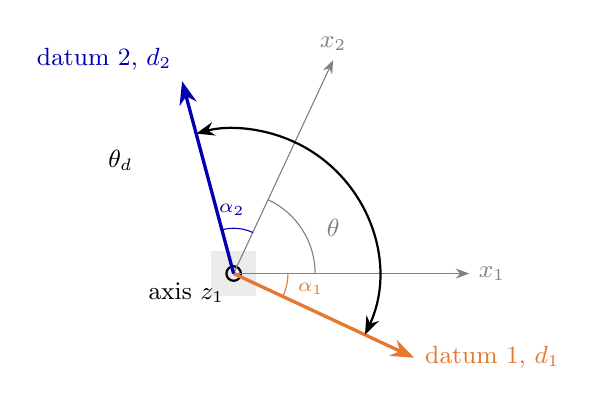
\begin{tikzpicture}[>=Stealth, scale=1.15]
  \fill[gray!15] (-0.25,-0.25) rectangle (0.25,0.25);
  \draw[thick] (0,0) circle (0.08);
  \node[below left] at (0,0) {\small axis $z_1$};
  % connector 1 x axis
  \draw[->, gray] (0,0) -- (2.6,0) node[right] {\small $x_1$};
  % connector 2 x axis
  \draw[->, gray] (0,0) -- ({2.6*cos(65)},{2.6*sin(65)}) node[above] {\small $x_2$};
  \draw[gray] (0.9,0) arc (0:65:0.9);
  \node[gray] at (1.1,0.5) {\small $\theta$};
  % datum 1
  \draw[->, very thick, bworange] (0,0) -- ({2.2*cos(-25)},{2.2*sin(-25)}) node[right] {\small datum 1, $d_1$};
  \draw[bworange] (0.6,0) arc (0:-25:0.6);
  \node[bworange] at (0.85,-0.17) {\scriptsize $\alpha_1$};
  % datum 2
  \draw[->, very thick, blue!70!black] (0,0) -- ({2.2*cos(105)},{2.2*sin(105)}) node[above left] {\small datum 2, $d_2$};
  \draw[blue!70!black] ({0.5*cos(65)},{0.5*sin(65)}) arc (65:105:0.5);
  \node[blue!70!black] at (-0.02,0.7) {\scriptsize $\alpha_2$};
  % datum angle
  \draw[<->, thick] ({1.6*cos(-25)},{1.6*sin(-25)}) arc (-25:105:1.6);
  \node at (-1.25,1.25) {\small $\theta_d$};
\end{tikzpicture}
\caption{Looking down the joint axis. Each datum sits at a fixed angle $\alpha_i$ in its own connector's frame,
because datum and connector are on the same part. The limit is applied to $\theta_d$, the angle from datum~1 to
datum~2.}
\label{fig:limit-datum}
\end{figure}

\paragraph{The arithmetic.} Turning part~2 by the joint angle $\theta$ turns datum~2 with it, so the datum angle is
\[
  \theta_d = \theta + \alpha_2 - \alpha_1 \qquad\Longrightarrow\qquad \theta = \theta_d + \theta_0,\quad
  \theta_0 = \alpha_1 - \alpha_2 .
\]
Here $\alpha_i$ is the angle of datum $i$'s direction, projected onto connector $i$'s $xy$ plane. The direction is a
face's normal, an edge's direction, or a datum's own $z$. Each $\alpha_i$ depends only on where the datum sits on its
own part, so $\theta_0$ does not change as the parts move. It is stored on the joint as \code{LimitAngleZero}
(read-only). A limit $\theta_d \in [\theta_{\min}, \theta_{\max}]$ becomes $\theta \in [\theta_{\min} + \theta_0,
\theta_{\max} + \theta_0]$ for the solver. Lengths work the same way, with the datums' heights $h_i$ along the axis:
$L_0 = h_1 - h_2$, stored as \code{LimitLengthZero}.

\paragraph{Drag backstop.} The solver stops at limits today, but nothing checked that it does. After each drag step,
BruceWorx now reads every limited joint itself. If a step would take a joint further past a limit, it is cut back:
the move is halved six times from the last good position, so the part stops within $1/64$ of one mouse step of the
limit. A plain solve that leaves a joint outside its limits now prints a warning in the Report view (``Hinge is at
120 deg, outside its limits (0 deg to 90 deg)''). Python can now drive a drag (\code{preDrag}, \code{doDragStep},
\code{postDrag}), which is how all of this is tested without a screen.

\paragraph{Keep parts where they are.} New checkbox in the joint panel, off by default, so a joint still moves one part
to line up the picks. Ticked, the joint is fitted to where the parts are: connector~2's offset takes up the
difference, $O_2' = O_2\,P_2^{-1}P_1$, where $P_i$ are the two connectors' world placements. Nothing moves, and the
joint still works: a revolute made this way turns about connector~1's axis. For a revolute, the angle then reads 0
where the parts were placed, so limits without datums count from the position the parts were built in (Fusion's
\emph{as-built} joint). The setting is stored on the joint (\code{KeepPosition}); ticking or unticking it while the
panel is open redoes the joint from the parts' original places. It is shown for Fixed, Revolute, Cylindrical, Slider
and Ball joints.

\paragraph{Verified headless.} 7 new Assembly tests (\file{AssemblyTests/TestBWJoints.py}), all passing with the 8
existing ones:
\begin{itemize}[nosep]
  \item a free drag to 170\,$^\circ$ and $-120\,^\circ$ without limits;
  \item a 0--90\,$^\circ$ limit stops a drag at 90 and at 0;
  \item the reading equals the face-to-face angle worked out from the geometry, at five angles;
  \item a 0--30\,$^\circ$ limit from two face datums stops a drag at 30 and at 0 measured face to face;
  \item no datums gives zero offsets;
  \item a joint moves the part by default, and with \emph{Keep parts where they are} it does not move it, even after a
        solve, and still turns about the joint.
\end{itemize}
The panel itself (checkbox, \emph{Pick datums}, reading) needs the screen: steps 14 and 16 of
section~\ref{sec:tonight}.

\paragraph{Still in \eref{ASM-03}.} Quick joint with type inference, pin-slot, limit sliders in the 3D view, datums on
the assembly origin or a third part (today both datums are on the joint's own two parts), and continuous angles past
$\pm 180\,^\circ$ (today a limit range lies within one turn).


\begin{epic}{ASM-03}{Joint UX \& limits}{M1}{\stProg}{FCB-P2A-03/04}
A pick-two-features \textbf{quick joint} that infers the joint type (cylinder + cylinder $\rightarrow$
revolute, plane + plane $\rightarrow$ planar, and so on), keyboard shortcuts, and \textbf{limit sliders} that the
solver honours while dragging. \textbf{Built 19 Oct (\S\ref{sec:joints}):} limits measured from datums, a drag
backstop at the limits, and \emph{Keep parts where they are}.
\emph{Acceptance:} the 2-DOF arm is assembled with quick joints, and limits stop the drag.
\end{epic}

\begin{epic}{ASM-04}{Exploded views \& BOM}{M1}{\stProg}{FCB-P2A-05/06}
Exploded-view presets, and a BOM with \textbf{P/N, Rev, Description, Material, Mass, Qty}, in
\emph{indented}, \emph{top-level} and \emph{flattened (parts only)} forms, exported to CSV. Configurations are
resolved per component (\eref{MOD-03}). The same BOM feeds the drawing table (\eref{DRW-02}) and Ops
(\eref{PDM-06}).
\textbf{Started 19 Oct 2026:} the columns come from the part-property schema (\S\ref{sec:partprops}), with
Mass and Material computed.
\emph{Acceptance:} the \code{LE-02001} BOM matches a hand count; the flattened BOM sums quantities.
\end{epic}

\paragraph{Theory: BOM explosion.} With edge multiplicities $q_{uv}$ in the assembly DAG, the total quantity
of part $p$ under top assembly $t$ is the sum over all paths of the product of multiplicities,
\[
  Q_t(p) = \sum_{\pi:\,t\rightsquigarrow p}\ \prod_{(u,v)\in\pi} q_{uv},
\]
computed in $O(|V|+|E|)$ by dynamic programming in topological order, $Q(v)=\sum_{u\to v}Q(u)\,q_{uv}$ with
$Q(t)=1$. The \emph{indented} BOM lists paths, and the \emph{flattened} BOM lists $Q_t(p)$ for leaf parts.
\emph{Where-used} (\eref{PDM-06}) is the same traversal on the reversed graph.

\begin{epic}{ASM-05}{Sub-assemblies}{M1}{\stTodo}{FCB-P2A-07}
Rigid vs.\ flexible sub-assemblies. A flexible one exposes its internal joints to the parent's solver; a
rigid one moves as one body. A fix-up macro converts between them.
\emph{Acceptance:} a flexible sub-assembly articulates inside \code{LE-02001}; a rigid one does not.
\end{epic}

\begin{epic}{ASM-06}{Interference \& clearance}{M1}{\stTodo}{FCB-P2A-08}
List every \textbf{clash} (positive common volume), \textbf{contact} (touching faces, zero volume) and
\textbf{clearance violation} (minimum distance below a threshold) between occurrences. Results are
highlighted in the view, with an ignore list for intended press fits and threads. The ECAD enclosure fit
(\eref{ECD-04}) reuses it.
\emph{Acceptance:} the bolt example in Figure~\ref{fig:clash} reports one clash, 4.0\,mm deep and 78.5\,mm$^3$.
\end{epic}

\begin{figure}[ht]
\centering
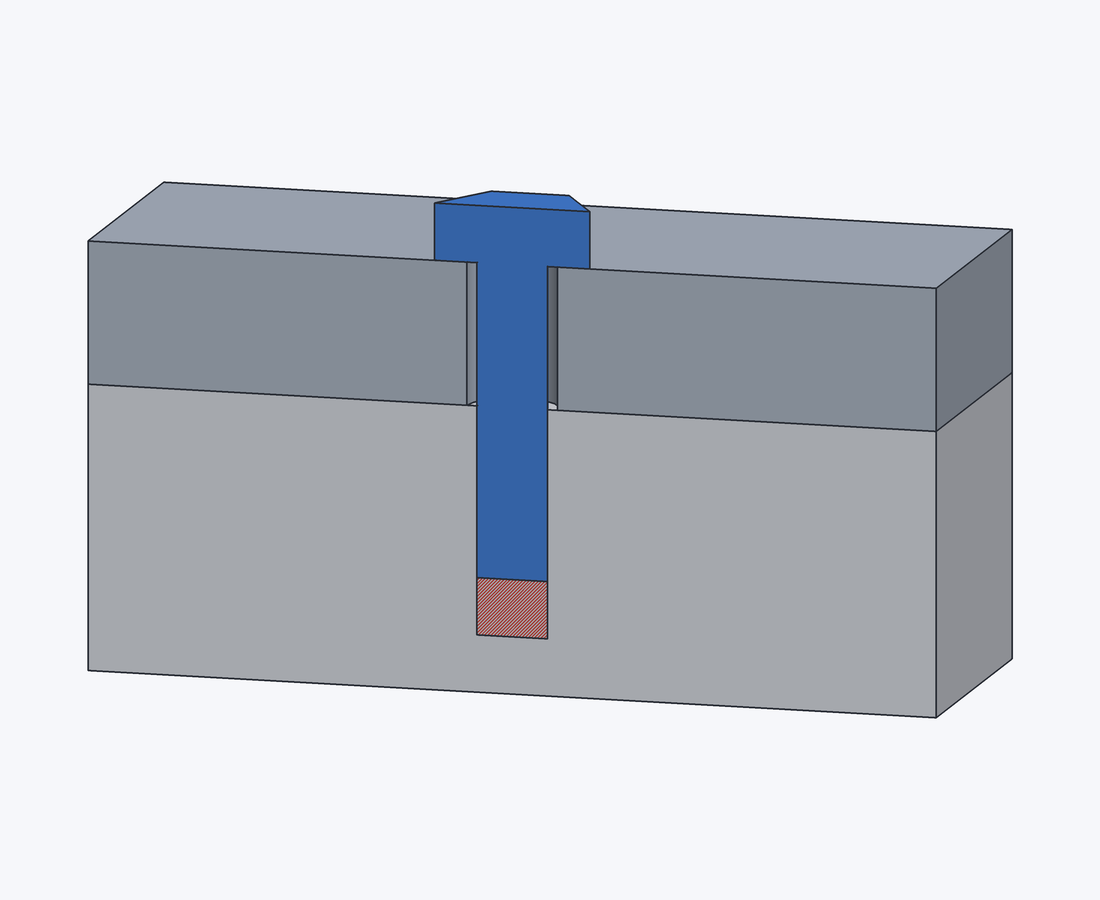
\includegraphics[width=0.5\linewidth]{fig/interference.png}
\caption{Half section of an M5 bolt that is 4\,mm too long for its 12\,mm blind hole. The clash volume
(red) is the Boolean common of bolt and block: 78.54\,mm$^3$ $=\pi\cdot2.5^2\cdot4$, computed in headless
FreeCAD. The section itself is the kind of view \eref{MOD-11} keeps in the model.}
\label{fig:clash}
\end{figure}

\paragraph{Theory: broad and narrow phase.} Checking all $\binom n2$ pairs exactly is too slow for a robot with
hundreds of parts. A \emph{broad phase} sorts the axis-aligned bounding boxes on each axis and sweeps,
reporting only pairs whose intervals overlap on all three axes. That takes $O(n\log n+k)$ for $k$ candidate pairs.
The \emph{narrow phase} runs the exact Boolean common (clash volume) or \code{distToShape} (clearance)
only on candidates. Contacts are separated from clashes by a volume tolerance $\varepsilon_V$ and a
distance tolerance $\varepsilon_d$. Pairs on the ignore list (threads, press fits) are filtered by occurrence
path, so they stay ignored after the assembly is rebuilt.

\begin{epic}{ASM-07}{In-context editing}{M5}{\stTodo}{(new)}
Edit a part while it is shown inside the assembly, referencing other parts' geometry (Fusion's in-place edit,
SolidWorks' in-context features). References become cross-document \code{SubShapeBinder}s and update when
the referenced part changes. They can be \textbf{locked} (frozen) or \textbf{broken}. A dashboard lists all
external references.
\emph{Acceptance:} bracket holes follow a moved motor mount across files.
\end{epic}

\begin{epic}{ASM-08}{Large-assembly mode}{M5}{\stTodo}{(new)}
Open a full robot quickly. That means \textbf{lightweight} loading (display data without the feature tree),
\textbf{selective open} (choose the sub-assemblies to load), cached tessellation, and level of detail
for small parts. The spike measures FreeCAD's existing partial-document loading for links first \verify.
\emph{Acceptance:} an assembly of more than 500 parts opens within a target set by the spike.
\end{epic}

\begin{epic}{ASM-09}{Smart fastener mating}{M5}{\stTodo}{FCB-P2R-04}
Select a hole pattern and a fastener type. The command recognises the holes (\eref{MOD-04} recognition,
\eref{MOD-05} data), picks size and length, inserts linked fasteners (and washers and nuts), and joints them.
This matches SolidWorks Toolbox smart fasteners and its 2026 fastener recognition.
\emph{Acceptance:} bolting a motor mount places and joints all its screws in one command.
\end{epic}

\paragraph{Theory: length selection.} For a through-bolt with clamp (grip) thickness $g$ into a tapped or
insert hole of usable depth $h$, the required engagement is $e\ge k\,d$, with $k\approx1.5$ in aluminium
and plastics, or the insert length for heat-set inserts. The chosen standard length is the smallest catalogue
length $L$ with
\[
  g + e \;\le\; L \;\le\; g + h - c ,
\]
where $c$ is the bottom clearance. If the set is empty, the command reports the conflict instead of
choosing. Figure~\ref{fig:clash} shows the failure it prevents.

\begin{epic}{ASM-10}{Dynamic motion study}{M5}{\stTodo}{FCB-P2A-10}
Beyond kinematic animation: \textbf{gravity, applied forces and torques, motor profiles, springs and
dampers, and contact}, integrated over time, with plots (position, velocity, reaction forces, motor
torque) and video export. The spike checks how much of the Ondsel (MbD) solver's dynamics can be used
\verify.
\emph{Acceptance:} the arm swinging under gravity matches the analytic pendulum period within 2\,\%.
\end{epic}

\paragraph{Theory: constrained multibody dynamics.} With generalised coordinates $\mathbf q$, mass
matrix $M(\mathbf q)$, applied forces $\mathbf Q$ and joint constraints $\Phi(\mathbf q,t)=\mathbf 0$,
\[
  M\ddot{\mathbf q}+\Phi_{\mathbf q}^{\!\top}\boldsymbol\lambda=\mathbf Q,\qquad \Phi(\mathbf q,t)=\mathbf 0,
\]
an index-3 differential-algebraic system. The Lagrange multipliers $\boldsymbol\lambda$ are the joint reaction
forces, which is what users want plotted to size motors. It is solved by index reduction to
$\Phi_{\mathbf q}\ddot{\mathbf q}=-(\Phi_{\mathbf q}\dot{\mathbf q})_{\mathbf q}\dot{\mathbf q}-2\Phi_{\mathbf qt}\dot{\mathbf q}-\Phi_{tt}$
with Baumgarte stabilisation, or with a generalised-$\alpha$ integrator on the index-3 form. Validation uses a
pendulum, $T=2\pi\sqrt{I_O/(m g\ell)}$.

%======================================================================
\section{Track DRW --- Drawings (ASME Y14.5, third-angle)}\label{sec:drw}
%======================================================================

TechDraw already covers projection groups, section, detail and broken views, dimensions (including chain
and coordinate extensions), balloons, weld and surface-finish symbols, template autofill, and
PDF/DXF export. The gaps are semantic. GD\&T frames are SVG symbols, not data. The BOM table is a
spreadsheet view. Thread callouts are drawn on the view, not read from the model. Nothing knows about
revisions. This track runs \textbf{in parallel from the start} and closes at M2.

\begin{figure}[ht]
\centering
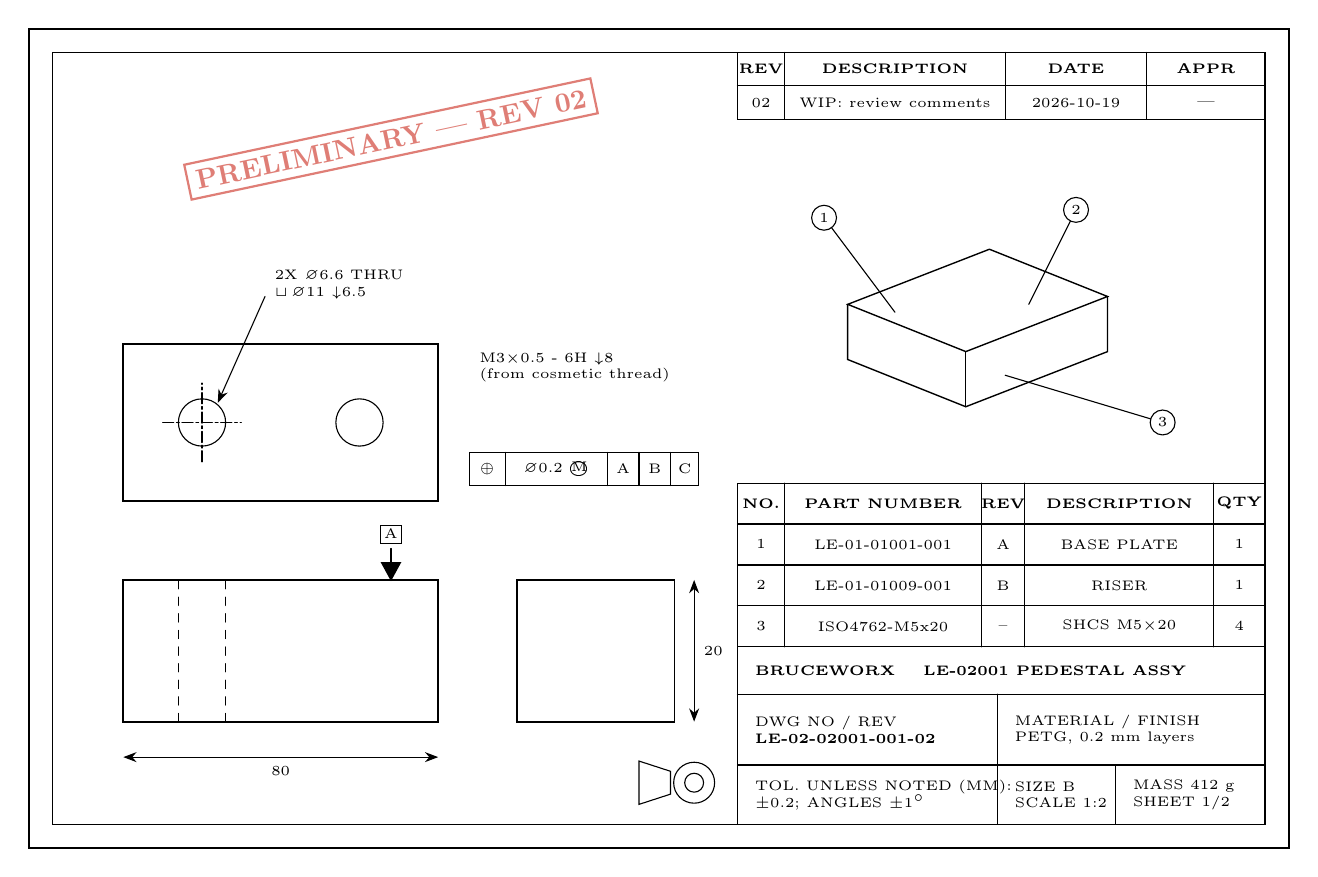
\begin{tikzpicture}[x=1cm,y=1cm,font=\tiny,line cap=round]
% sheet border
\draw[line width=0.8pt] (0,0) rectangle (16,10.4);
\draw (0.3,0.3) rectangle (15.7,10.1);
% revision block, top right
\draw (9.0,9.25) rectangle (15.7,10.1); \draw (9.0,9.68) -- (15.7,9.68);
\foreach \x in {9.6,12.4,14.2} \draw (\x,9.25) -- (\x,10.1);
\node at (9.3,9.89) {\bfseries REV}; \node at (11.0,9.89) {\bfseries DESCRIPTION}; \node at (13.3,9.89) {\bfseries DATE}; \node at (14.95,9.89) {\bfseries APPR};
\node at (9.3,9.46) {02}; \node at (11.0,9.46) {WIP: review comments}; \node at (13.3,9.46) {2026-10-19}; \node at (14.95,9.46) {---};
% PRELIMINARY stamp
\node[rotate=12,text=bwred!70,font=\bfseries\normalsize,draw=bwred!70,line width=0.8pt,inner sep=3pt] at (4.6,9.0) {PRELIMINARY --- REV 02};
% third-angle views: front bottom-left, top above it, right view to its right
\draw[line width=0.6pt] (1.2,1.6) rectangle (5.2,3.4);
\draw[line width=0.6pt] (1.2,4.4) rectangle (5.2,6.4);
\draw[line width=0.6pt] (6.2,1.6) rectangle (8.2,3.4);
\draw[dashed] (1.9,1.6) -- (1.9,3.4); \draw[dashed] (2.5,1.6) -- (2.5,3.4);
\draw (2.2,5.4) circle (0.3); \draw (4.2,5.4) circle (0.3);
\draw[dash pattern=on 4pt off 1pt on 1pt off 1pt] (2.2,4.9)--(2.2,5.9) (1.7,5.4)--(2.7,5.4);
% dimensions
\draw[<->,>=Stealth] (1.2,1.15) -- node[below]{80} (5.2,1.15);
\draw[<->,>=Stealth] (8.45,1.6) -- node[right]{20} (8.45,3.4);
% datum A on the top face of the front view
\draw[fill=black] (4.6,3.4) -- ++(-0.12,0.22) -- ++(0.24,0) -- cycle; \draw (4.6,3.62) -- (4.6,3.8);
\node[draw,inner sep=1.5pt] at (4.6,3.98) {A};
% hole callout and thread note
\draw[->,>=Stealth] (3.0,7.0) -- (2.4,5.65);
\node[anchor=west,align=left] at (3.0,7.15) {2X $\varnothing$6.6 THRU\\ $\sqcup\,\varnothing$11 $\downarrow$6.5};
\node[anchor=west,align=left] at (5.6,6.1) {M3$\times$0.5 - 6H $\downarrow$8\\ (from cosmetic thread)};
% feature control frame
\begin{scope}[shift={(5.6,4.6)}]
\draw (0,0) rectangle (2.9,0.42);
\draw (0.45,0)--(0.45,0.42) (1.75,0)--(1.75,0.42) (2.15,0)--(2.15,0.42) (2.55,0)--(2.55,0.42);
\node at (0.22,0.21) {$\oplus$}; \node at (1.1,0.21) {$\varnothing$0.2 \textcircled{\tiny M}};
\node at (1.95,0.21) {A}; \node at (2.35,0.21) {B}; \node at (2.73,0.21) {C};
\end{scope}
% isometric with balloons, right middle
\draw[line width=0.5pt] (10.4,6.9) -- (12.2,7.6) -- (13.7,7.0) -- (11.9,6.3) -- cycle;
\draw[line width=0.5pt] (10.4,6.9) -- (10.4,6.2) -- (11.9,5.6) -- (13.7,6.3) -- (13.7,7.0);
\draw (11.9,6.3)--(11.9,5.6);
\foreach \n/\x/\y/\tx/\ty in {1/11.0/6.8/10.1/8.0, 2/12.7/6.9/13.3/8.1, 3/12.4/6.0/14.4/5.4}{
  \draw (\x,\y) -- (\tx,\ty); \node[circle,draw,fill=white,inner sep=1pt,minimum size=9pt] at (\tx,\ty) {\n};}
% parts list (ASME Y14.34) above the title block
\begin{scope}[shift={(9.0,2.55)}]
\draw (0,0) rectangle (6.7,2.08);
\foreach \y in {0.52,1.04,1.56} \draw (0,\y)--(6.7,\y);
\foreach \x in {0.6,3.1,3.65,6.05} \draw (\x,0)--(\x,2.08);
\node at (0.3,1.82) {\bfseries NO.}; \node at (1.85,1.82) {\bfseries PART NUMBER}; \node at (3.375,1.82) {\bfseries REV};
\node at (4.85,1.82) {\bfseries DESCRIPTION}; \node at (6.375,1.82) {\bfseries QTY};
\node at (0.3,1.30) {1}; \node at (1.85,1.30) {LE-01-01001-001}; \node at (3.375,1.30) {A}; \node at (4.85,1.30) {BASE PLATE}; \node at (6.375,1.30) {1};
\node at (0.3,0.78) {2}; \node at (1.85,0.78) {LE-01-01009-001}; \node at (3.375,0.78) {B}; \node at (4.85,0.78) {RISER}; \node at (6.375,0.78) {1};
\node at (0.3,0.26) {3}; \node at (1.85,0.26) {ISO4762-M5x20}; \node at (3.375,0.26) {--}; \node at (4.85,0.26) {SHCS M5$\times$20}; \node at (6.375,0.26) {4};
\end{scope}
% title block, bottom right
\begin{scope}[shift={(9.0,0.3)}]
\draw (0,0) rectangle (6.7,2.25);
\draw (0,0.75)--(6.7,0.75) (0,1.65)--(6.7,1.65) (3.3,0)--(3.3,1.65) (4.8,0)--(4.8,0.75);
\node[anchor=west] at (0.1,1.95) {\bfseries BRUCEWORX \quad LE-02001 PEDESTAL ASSY};
\node[anchor=west,align=left] at (0.1,1.2) {DWG NO / REV\\\bfseries LE-02-02001-001-02};
\node[anchor=west,align=left] at (3.4,1.2) {MATERIAL / FINISH\\ PETG, 0.2 mm layers};
\node[anchor=west,align=left] at (0.1,0.37) {TOL.\ UNLESS NOTED (MM):\\ $\pm$0.2; ANGLES $\pm$1$^\circ$};
\node[anchor=west,align=left] at (3.4,0.37) {SIZE B\\ SCALE 1:2};
\node[anchor=west,align=left] at (4.9,0.37) {MASS 412 g\\ SHEET 1/2};
\end{scope}
% third-angle projection symbol, left of the title block
\begin{scope}[shift={(7.75,0.55)}]
\draw (0,0) -- (0.4,0.13) -- (0.4,0.42) -- (0,0.55) -- cycle; \draw (0.7,0.275) circle (0.12); \draw (0.7,0.275) circle (0.26);
\end{scope}
\end{tikzpicture}
\caption{Target ASME B-size sheet (schematic). Third-angle views and symbol; hole and thread callouts
generated from model data; a semantic feature control frame against datums A--C; balloons tied to the
parts list; revision block and PRELIMINARY stamp driven by the PDM state (numeric rev 02 = not yet
released); title block filled from item metadata, printed as \code{P/N-REV}.}
\label{fig:sheet-mock}
\end{figure}

\begin{epic}{DRW-01}{ASME templates \& title block}{M2}{\stTodo}{FCB-P2-06/07/08}
ANSI A--D sheet templates with the third-angle symbol, a general tolerance block, and fields for P/N, revision,
title, material, finish, mass, scale, sheet and approvals. Fields fill from PDM item metadata
(\eref{PDM-02}) through TechDraw's existing autofill, which is extended for the new keys. The \code{LE-01001}
sample drawing (overall size, thickness, print Z, PETG/ABS, heat-set inserts) is the first user.
\emph{Acceptance:} the \code{LE-01001} drawing fills every field automatically.
\end{epic}

\begin{epic}{DRW-02}{Associative BOM table \& balloons}{M2}{\stTodo}{FCB-P2A-06}
A native TechDraw \textbf{parts list} object (ASME Y14.34 columns: item, P/N, rev, description,
material, qty) bound to the assembly BOM (\eref{ASM-04}), replacing the spreadsheet view. Balloons bind to
\emph{occurrences}, so their numbers follow the item numbers when rows are added, sorted or removed.
\emph{Acceptance:} adding a part updates the table and keeps every balloon number correct.
\end{epic}

\begin{epic}{DRW-03}{GD\&T \& datums (ASME Y14.5)}{M2}{\stTodo}{(new)}
Feature control frames, datum feature symbols, datum targets and basic dimensions as \textbf{objects}
that reference model geometry. They are validated (every referenced datum exists, modifiers are legal for the
characteristic), and they survive model edits through TNP-safe references.
\emph{Acceptance:} a frame referencing a missing datum is flagged; frames survive a model change.
\end{epic}

\paragraph{Theory: a feature control frame is a sentence.} Y14.5 frames follow a small grammar:
\begin{lstlisting}
fcf        := characteristic zone ( '|' datumRef ){0,3}
zone       := [ 'DIA' | 'SDIA' ] value [ material ] [ 'P' value ] [ 'F' | 'ST' | 'T' ]
material   := '(M)' | '(L)'          ; MMC / LMC (RFS is the default)
datumRef   := letter [ material ] ( '-' letter [ material ] )*
\end{lstlisting}
Validation rules: form tolerances (flatness, straightness, circularity, cylindricity) take \emph{no} datums;
orientation tolerances need at least one; position needs datums unless the frame is a pattern-locating tolerance
that is explicitly datum-free; and the material modifier \textcircled{\small M} applies only to features of size. Storing the
frame as a parsed structure, not as text, is what makes these checks possible. It also allows STEP AP242
semantic PMI export later.

\begin{epic}{DRW-04}{Hole \& thread callouts from the model}{M2}{\stTodo}{(new)}
Generate callout text from \code{Hole} features and cosmetic threads (\eref{MOD-05}): quantity, diameter,
THRU or depth, counterbore $\sqcup$, countersink $\vee$, thread size, pitch, class and depth. Callouts update
when the hole changes. Hole tables (ordinate positions) come from the same data.
\emph{Acceptance:} callouts update when the hole spec changes.
\end{epic}

\begin{epic}{DRW-05}{Revision table \& release stamp}{M2}{\stTodo}{(new)}
The revision block is filled from the item's change history (\eref{PDM-05}): ECO number, description, date and
approver per letter revision. A \textbf{PRELIMINARY} stamp shows while the revision is numeric (01, 02, \ldots).
The title block prints \code{P/N-REV}.
\emph{Acceptance:} releasing rev A removes the stamp and adds the revision row.
\end{epic}

\begin{epic}{DRW-06}{Auto-generate drawing}{M2}{\stTodo}{(new)}
One command makes a first-pass drawing: sheet size and scale, the standard views, an isometric, hole callouts,
and the key dimensions. The user then edits it. SolidWorks 2026 ships an equivalent, AutoGenerate Drawing.
\emph{Acceptance:} on the corpus parts, a reviewer keeps at least 70\,\% of the generated dimensions.
\end{epic}

\paragraph{Theory: choosing views and dimensions.}
\begin{enumerate}
  \item \textbf{Front view.} Among the six principal directions $\pm\mathbf e_x,\pm\mathbf e_y,\pm\mathbf e_z$
        of the part's oriented bounding box, choose the one maximising
        $\alpha\,A_{\text{proj}}+\beta\,N_{\text{visible edges}}-\gamma\,N_{\text{hidden edges}}$, with
        ties broken by the longest extent horizontal. The other views follow from third-angle
        projection: top above, right to the right.
  \item \textbf{Needed views.} Add a view only if it shows features (holes, steps) whose axis is
        perpendicular to it and which no earlier view shows true size. A part with all holes on one axis gets
        two views, not three.
  \item \textbf{Scale and sheet.} The smallest standard sheet (A--D) and the largest standard scale such that
        the view group fits within 80\,\% of the drawing area.
  \item \textbf{Dimensions.} Overall extents first, then hole positions as ordinate or baseline dimensions
        from the datum features (the largest planar faces, in order), then sizes through callouts. Nothing is
        dimensioned twice: each model parameter maps to at most one dimension.
\end{enumerate}

\begin{epic}{DRW-07}{Sheet-metal flat \& cut-list drawings}{M3}{\stTodo}{(new)}
A flat-pattern view with bend lines, direction and angle, a bend table (bend, direction, angle, radius,
K-factor), and the weldment cut-list table from \eref{MOD-07}.
\emph{Acceptance:} the bracket drawing in Figure~\ref{fig:sheet} shows the flat and the table.
\end{epic}

\begin{epic}{DRW-08}{Publish PDF/DXF}{M2}{\stTodo}{(new)}
Vector PDF and DXF export of every drawing in a BOM, with file names \code{P/N-REV.pdf}. It feeds the
release package (\eref{MFG-04}).
\emph{Acceptance:} one command publishes every drawing of \code{LE-02001}.
\end{epic}

%======================================================================
\section{Track PDM --- Part and drawing management}\label{sec:pdm}
%======================================================================

FreeCAD has no PDM: no vault, check-out, revision, lifecycle, where-used or release. Fusion has
versions in its cloud plus the Manage extension (part numbering, lifecycle, change orders, BOM release).
SolidWorks has PDM Standard and Professional (vault, check-in/out, workflows, revisions, BOMs). Searches
for an open-source PDM with a working FreeCAD check-in workflow found only early or narrow projects
(FreePDM, a concept; a small Taack-based PLM; LibrePLM, with a Windows-only connector). This track
therefore \textbf{starts with an evaluation}, as decided, and specifies the data model and lifecycle
independently of where they end up stored.

\begin{epic}{PDM-01}{PDM evaluation \& decision}{M2}{\stDone}{(new)}
Compare four architectures against weighted criteria and record the decision. \textbf{Decided 19 Oct 2026
(\S\ref{sec:pdm-decision}):} a vault in any folder, iCloud Drive first, opened through a \file{.bwvault} ref file;
one writer at a time for now. The folder layout is designed so a sync service has nothing to conflict over.
\end{epic}

%======================================================================
\subsection{BW-PDM-01 --- Decision: a vault in a folder (19 Oct 2026)}\label{sec:pdm-decision}
%======================================================================

\textbf{Decision (your answer, 19 Oct).} The vault lives in any folder you choose and builds itself there; a ref
file lets a reader view and drive it; the backend is that folder, most likely in iCloud, so it moves easily to
another provider. Scope, also 19 Oct: \textbf{one FreeCAD at a time}; simultaneous edits from several instances are
not part of this step.

\paragraph{Layout.} A sync service makes conflict copies only when \emph{the same file} changes in two places,
or changes again while an earlier version is still uploading. The vault is laid out so that never happens:

\begin{center}
\small
\begin{tabularx}{\linewidth}{@{}lX@{}}
\toprule
Path in the vault folder & Rule\\
\midrule
\file{<name>.bwvault} & The \textbf{ref file}. Identifies the vault (name, id, format version). Written once.
  Today \code{bw-hooks vault status --vault <file>} opens it; the FreeCAD panel (\eref{PDM-04}) will open it
  from File $\rightarrow$ Open or a double-click.\\
\file{objects/ab/<sha256>.FCStd} & Every checked-in file version, named by its content hash. \textbf{Written once,
  never changed}; written under a \file{.tmp} name (which iCloud does not sync) and renamed when complete; checked
  against its hash when read.\\
\file{journal/<user>@<mac>.jsonl} & Every action (create, check out, check in, submit, approve, ECR, ECO, BOM) as
  one line. \textbf{Append-only, and only that user on that Mac writes it.} The state is rebuilt by replaying the
  lines through the reference model (\eref{PDM-02}), so the lifecycle rules are identical.\\
working folder (outside the vault) & Where FreeCAD opens and saves while you work. Check-in copies the file into
  \file{objects/}; check-out copies the latest one out. Saving every few minutes never touches the vault.\\
\bottomrule
\end{tabularx}
\end{center}

If a sync service makes a copy anyway (iCloud \file{x 2.jsonl}, Dropbox \file{x (conflicted copy).jsonl},
Syncthing \file{x.sync-conflict-\ldots}), the reader reads \emph{every} journal file and keeps each event once, so a
copy neither loses nor doubles anything. A half-synced last line is skipped until the rest arrives; a journal line
whose file has not downloaded yet is reported as ``not synced yet'' rather than an error. Moving to another
provider means moving the folder.

\paragraph{Built and tested headless.} \file{addons/BruceWorx/bruceworx/pdm\_folder.py} with the command line
\code{bw-hooks vault} (actions \code{init}, \code{status}, \code{create}, \code{checkout}, \code{checkin},
\code{undo-checkout}, \code{submit}, \code{approve}, \code{reject}, \code{fetch}). The 12 lifecycle
and BOM contract tests of \eref{PDM-02} pass unchanged against a real folder, plus 17 folder tests: reopening rebuilds
identical state; a refused action writes nothing; versions are never rewritten; the released revision freezes its
file; damaged files are caught; three kinds of duplicate journal, an emptied journal, a half-written line, a missing
download, and a duplicated ref file. The OpenAPI file stays as the list of operations; the folder vault
implements them locally, and a server can implement them later.

\subsubsection*{iCloud: what we found}

\begin{description}[leftmargin=0pt]
  \item[Your Documents folder is in iCloud.] Desktop \& Documents sync is on
        (\file{\textasciitilde/Library/Mobile Documents/com\textasciitilde apple\textasciitilde CloudDocs/Documents} points
        at \file{\textasciitilde/Documents}), so this repository is synced.
  \item[Where the duplicates are.] 1\,488 numbered copies, \emph{all} in machine-written trees: build output
        (\file{build/release/share}, \file{src}) and 21 inside \file{.git} (\file{HEAD 2}, \file{index 2},
        \file{config 2}). None among the hand-edited sources. They arrived in bursts at clone and build times
        (937 in one minute on 15 Oct). The copies hold older contents: iCloud kept the version it had while the
        build was replacing thousands of files.
  \item[Single-file saves did not reproduce it.] On 19 Oct, 120 rapid rewrites of three files (save by rename,
        delete and recreate, overwrite in place) and three write passes over 3\,000 small files on this Mac produced no
        copies. The trigger is heavy, fast, machine-made churn, which is exactly what the vault never does.
  \item[Excluding a folder works on this Mac (macOS 27.2).] A folder whose name ends in \file{.nosync}, or one
        carrying the attribute \code{com.apple.fileprovider.ignore\#P}, is reported by \code{fileproviderctl} as
        \code{isExcludedFromSync = 1} and is not uploaded. Both are undocumented by Apple and could change; the
        \file{.nosync} name is the more widely used.
  \item[Storage optimisation.] With ``Optimise Mac Storage'' on, iCloud can evict files to save space; opening one
        waits for a download and fails offline. For the vault folder, turn it off or use Finder's \emph{Keep
        Downloaded} on the folder.
  \item[Sharing needs a folder in iCloud Drive itself.] Apple does not share the Desktop or Documents folders
        themselves; a shared folder has to sit in iCloud Drive. Folder sharing needs macOS 10.15.4, iOS 13.4 or
        iCloud for Windows 11.1 or later.
\end{description}

\paragraph{Recommended setup (yours to apply).}
\begin{enumerate}[nosep]
  \item Put the vault in \textbf{iCloud Drive, not Documents}, e.g.\ \file{iCloud Drive/BruceWorx Vault/}. A vault in
        Documents works for you alone, but a vault in iCloud Drive can be shared later without moving it.
  \item Keep the working folder out of sync: \file{\textasciitilde/BruceWorx Work} (outside Documents), or a
        \file{Work.nosync} folder.
  \item Turn on \emph{Keep Downloaded} for the vault folder.
  \item This repository: move it out of Documents (for example to \file{\textasciitilde/Developer}), or at least
        exclude \file{build} and \file{.pixi}. Git inside iCloud is a known way to damage a repository, and its
        \file{.git} already holds 21 duplicate files. Not changed here; it is your machine and your call.
\end{enumerate}

\paragraph{The repository, looked at again (19 Oct).} \code{git fsck} is clean, but the duplicates show the risk.
\file{.git/HEAD 2} reads \code{ref: refs/heads/.invalid} and \file{.git/config 2} has lost the branch and submodule
settings: both are the half-written state from the clone. Had iCloud settled those conflicts the other way, the
repository would have lost track of its branch and of GitHub. Excluding only \file{build} and \file{.pixi} would
leave this in place, and a branch switch or rebase rewrites thousands of source files at once, which is the same
burst that made the copies.
\begin{description}[leftmargin=0pt,nosep]
  \item[Recommended.] Repository in \file{\textasciitilde/Developer}, outside iCloud. Its off-machine copy is GitHub
        (a pushed work branch) plus Time Machine, both of which understand git. The vault, the one thing that needs
        file sync, goes in \file{iCloud Drive/BruceWorx Vault/}, which is built for it.
  \item[Not recommended.] Keeping the repository in Documents with \file{.git}, \file{build} and \file{.pixi}
        excluded. The sources would still sync, but iCloud's copy would be sources without history, and the exclusion
        relies on undocumented behaviour.
\end{description}
Moving needs a fresh \code{pixi install} and a full build, because both store absolute paths. Uncommitted work should
be pushed to a branch first, so that it exists somewhere other than this Mac.

\paragraph{Limits of this step.} One writer at a time. Journals are per user and Mac, so a second Mac or a second
person can be added later, but two people editing at the same moment are not reconciled, and the check-out lock is a
record in the journal, not a server lock. When a team needs that, the same operations move behind a server
(option A below) without changing the files.

%======================================================================
\subsection{BW-PDM-01 --- Evaluation memo (19 Oct 2026, before the decision)}\label{sec:pdm-eval}
%======================================================================

\textbf{Status.} Kept for the record. Option C was scored as a \emph{plain} shared folder with FreeCAD files
saved straight into it; the decision above is a folder vault built to avoid exactly the weaknesses scored here.

\begin{center}
\scriptsize
\setlength{\tabcolsep}{3pt}
\renewcommand{\code}[1]{\texttt{#1}}
\begin{longtable}{@{}>{\raggedright\arraybackslash}p{2.3cm}>{\raggedright\arraybackslash}p{3.4cm}>{\raggedright\arraybackslash}p{3.4cm}>{\raggedright\arraybackslash}p{3.2cm}>{\raggedright\arraybackslash}p{3.3cm}@{}}
\toprule
Evidence & A. Ops is the PLM & B. Ops + Git LFS & C. Vault on a shared folder & D. Open-source PLM\\
\midrule\endhead
\bottomrule\endfoot
Platform today & Ops = Next.js 16 on Railway (\code{bruceworks}); task API and auth are being built on branches (staging \code{/api/tasks} answers 401) & git-lfs 3.8 installed here; GitHub hosts the repos already & Folder on NAS or cloud drive & DocDokuPLM (Java), LibrePLM (Odoo; Windows-only connector), FreePDM (concept, no releases)\\
File storage cost & Railway bucket: \$0.015/GB-month, S3 operations and bucket egress free & GitHub Free/Pro: 10\,GiB storage + 10\,GiB bandwidth per month, then \$0.07/GiB storage, \$0.0875/GiB bandwidth; Team: 250\,GiB each & Disk you own & Self-hosting + upkeep\\
Locking & Server-side lease per item (contract: \code{/checkout}, \code{/checkin}) & \code{git lfs lock}: others cannot push a locked file & None real. \textbf{This repo already shows the failure:} iCloud left conflict copies (\file{BruceWorx 2.py}, \file{build 2.ninja}) instead of refusing & Built in\\
Lifecycle and ECO & Exactly the reference model (\file{bruceworx/pdm.py}) & In Ops (same model); Git only versions files & Must be built in the FreeCAD client & Configurable; fit with Y14.35 + ECR/ECO unproven\\
Multi-file assembly links & Client maps vault paths to a local workspace & Repo-relative paths work as they are & Share-relative paths & Needs a FreeCAD connector (none exists)\\
BOM and where-used & Ops (graph queries) & Ops & Client index & Built in\\
Agents / MCP & One API for FreeCAD, agents and the website & Git + Ops API & Weak & Varies\\
Main risk & Effort: we own a vault & Two systems to keep in step; CAD users must use Git (or a client that hides it) & Silent duplicates, no server truth & Connector effort, maintenance, Windows bias\\
\end{longtable}
\end{center}

\begin{center}
\small
\begin{tabular}{@{}lccccc@{}}
\toprule
Criterion (proposed weight) & A & B & C & D\\
\midrule
Data integrity and locking (25\,\%) & 5 & 4 & 2 & 4\\
Lifecycle fit, Y14.35 + ECR/ECO (20\,\%) & 5 & 3 & 3 & 3\\
Multi-file references (15\,\%) & 4 & 5 & 4 & 2\\
BOM and where-used (15\,\%) & 5 & 4 & 2 & 5\\
Build effort, higher is less work (10\,\%) & 2 & 3 & 3 & 2\\
Agent / API access (10\,\%) & 5 & 4 & 2 & 3\\
Running cost (5\,\%) & 5 & 3 & 5 & 4\\
\midrule
\textbf{Weighted score} & \textbf{4.55} & \textbf{3.80} & \textbf{2.75} & \textbf{3.35}\\
\bottomrule
\end{tabular}
\end{center}

\paragraph{Recommendation at the time.} Prototype \textbf{A} and \textbf{B} on \code{LE-02001}, then decide.
Rule out \textbf{C}: its failure mode (silent duplicates) is already visible in this repository. Keep \textbf{D}
as a fallback only, since none has a FreeCAD connector. Either A or B uses the same reference model and contract
(\eref{PDM-02}), so no work is lost whichever wins.

\paragraph{Prototype plan (not pursued after the decision).}
\begin{description}[leftmargin=0pt]
  \item[A.] A small service implementing \file{docs/pdm-openapi.yaml} over \file{bruceworx/pdm.py}, with files in
        a Railway bucket and SHA-256 content addressing. Run the contract tests against it, then check in the
        \code{LE-02001} tree and walk one ECO. Creating the bucket and service is an outward-facing change on your
        Railway account, so it waits for you.
  \item[B.] A private GitHub repository with LFS tracking for \code{*.FCStd} and locking turned on. Two clones
        play two engineers; measure lock conflicts and the clone size after ten revisions of the pedestal.
\end{description}


\subsection{Data model}

\begin{figure}[ht]
\centering
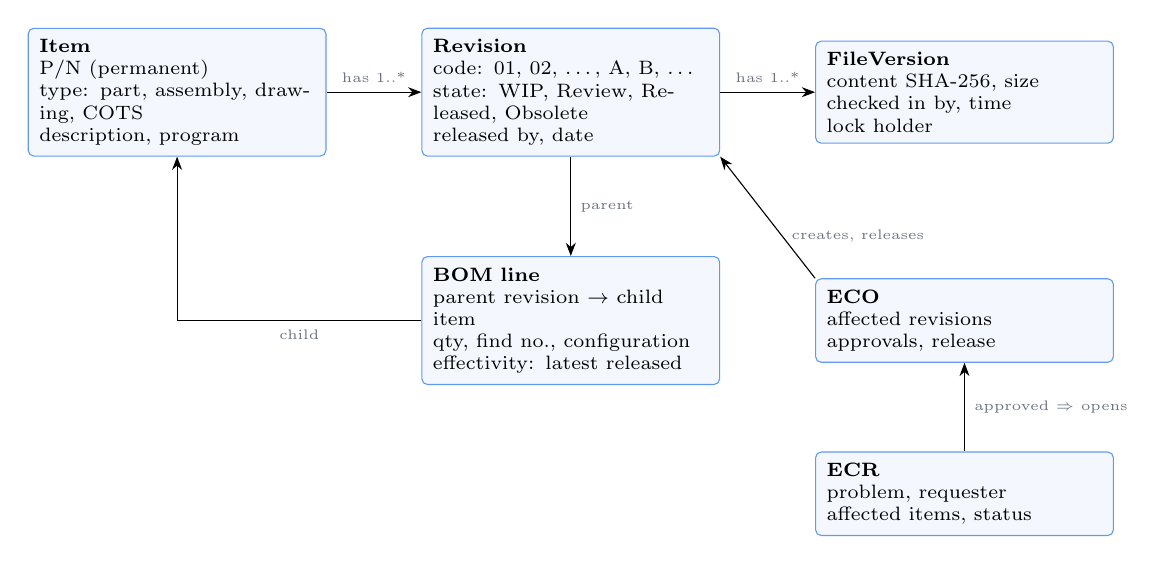
\begin{tikzpicture}[>=Stealth,
  ent/.style={draw=bwblue!70,fill=bwblue!5,rounded corners=2pt,align=left,font=\scriptsize,inner sep=4pt,text width=3.5cm},
  rel/.style={font=\tiny\color{bwgrey}}]
\node[ent] (item) at (0,0) {\textbf{Item}\\P/N (permanent)\\type: part, assembly, drawing, COTS\\description, program};
\node[ent] (rev) at (5.0,0) {\textbf{Revision}\\code: 01, 02, \ldots, A, B, \ldots\\state: WIP, Review, Released, Obsolete\\released by, date};
\node[ent] (fv) at (10.0,0) {\textbf{FileVersion}\\content SHA-256, size\\checked in by, time\\lock holder};
\node[ent] (bom) at (5.0,-2.9) {\textbf{BOM line}\\parent revision $\rightarrow$ child item\\qty, find no., configuration\\effectivity: latest released};
\node[ent] (eco) at (10.0,-2.9) {\textbf{ECO}\\affected revisions\\approvals, release};
\node[ent] (ecr) at (10.0,-5.1) {\textbf{ECR}\\problem, requester\\affected items, status};
\draw[->] (item) -- node[rel,above]{has 1..*} (rev);
\draw[->] (rev) -- node[rel,above]{has 1..*} (fv);
\draw[->] (rev) -- node[rel,right]{parent} (bom);
\draw[->] (bom.west) -| node[rel,pos=0.25,below]{child} (item.south);
\draw[->] (ecr) -- node[rel,right]{approved $\Rightarrow$ opens} (eco);
\draw[->] (eco.north west) -- node[rel,right,pos=0.35]{creates, releases} (rev.south east);
\end{tikzpicture}
\caption{PDM data model. The P/N belongs to the \emph{Item} and never changes. Revisions carry the state.
File versions are content-addressed. BOM lines point from a parent \emph{revision} to a child \emph{item},
so a released assembly picks up the child's latest released revision unless it is pinned.}
\label{fig:pdm-model}
\end{figure}

\begin{epic}{PDM-02}{Data model \& lifecycle spec}{M2}{\stProg}{(new)}
Specify Figure~\ref{fig:pdm-model} and the lifecycle in Figure~\ref{fig:lifecycle-sm} as an API contract
(OpenAPI) that any storage option implements. A drawing is its own \emph{Item}, numbered like its part, whose
revision moves \emph{with} the part's: one ECO releases both.
\textbf{Drafted 19 Oct 2026:} reference model \file{addons/BruceWorx/bruceworx/pdm.py} (revision sequences,
lifecycle, ECR/ECO, drawing coupling, BOM explosion, where-used, cycle rejection) with 18 contract tests in
\file{tests/test\_pdm.py}, and the API contract \file{addons/BruceWorx/docs/pdm-openapi.yaml} (17 endpoints,
including check-in/out and locks).
\emph{Acceptance:} spec approved; every transition in Figure~\ref{fig:lifecycle-sm} has an endpoint and a test.
\end{epic}

\subsection{Lifecycle and revisions}\label{sec:lifecycle}

\begin{figure}[ht]
\centering
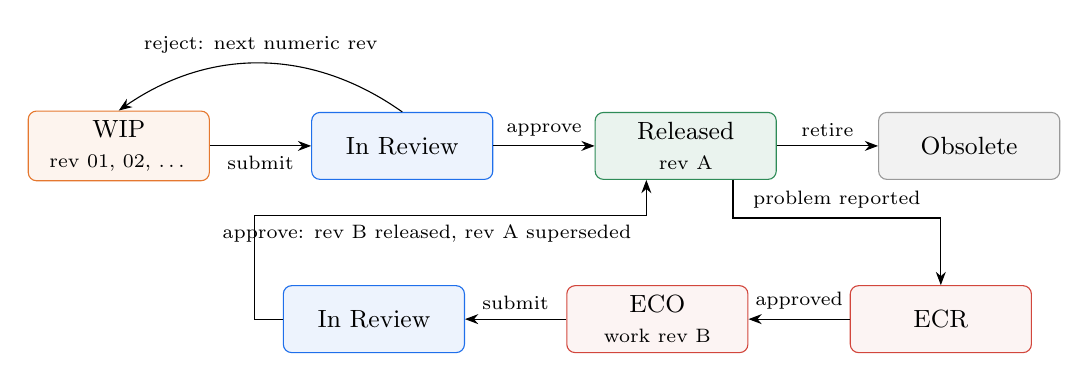
\begin{tikzpicture}[>=Stealth,x=3.6cm,y=-2.2cm,
  s/.style={draw,rounded corners=3pt,minimum width=2.3cm,minimum height=0.85cm,align=center,font=\small},
  wip/.style={s,draw=bworange,fill=bworange!8},rv/.style={s,draw=bwblue,fill=bwblue!8},
  rl/.style={s,draw=bwgreen,fill=bwgreen!10},ob/.style={s,draw=black!40,fill=black!5},
  ch/.style={s,draw=bwred,fill=bwred!6},
  t/.style={font=\scriptsize,align=center}]
\node[wip] (wip) at (0,0) {WIP\\\scriptsize rev 01, 02, \ldots};
\node[rv]  (rv)  at (1,0) {In Review};
\node[rl]  (rl)  at (2,0) {Released\\\scriptsize rev A};
\node[ob]  (ob)  at (3,0) {Obsolete};
\node[ch]  (ecr) at (2.9,1) {ECR};
\node[ch]  (eco) at (1.9,1) {ECO\\\scriptsize work rev B};
\node[rv]  (rv2) at (0.9,1) {In Review};
\draw[->] (wip) -- node[t,below]{submit} (rv);
\draw[->] (rv.north) to[bend right=35] node[t,above]{reject: next numeric rev} (wip.north);
\draw[->] (rv) -- node[t,above]{approve} (rl);
\draw[->] (rl) -- node[t,above]{retire} (ob);
\draw[->] ([xshift=0.6cm]rl.south) -- ++(0,0.22) -| node[t,pos=0.25,above]{problem reported} (ecr.north);
\draw[->] (ecr) -- node[t,above]{approved} (eco);
\draw[->] (eco) -- node[t,above]{submit} (rv2);
\draw[->] (rv2.west) -- ++(-0.1,0) |- node[t,pos=0.72,below]{approve: rev B released, rev A superseded} ($([xshift=-0.5cm]rl.south)+(0,-0.45cm)$) -- ([xshift=-0.5cm]rl.south);
\end{tikzpicture}
\caption{Lifecycle. Pre-release revisions are numeric (ASME Y14.35 practice) and every review rejection
increments them. The first approval releases rev A. After that, letters change only through an approved ECR
$\rightarrow$ ECO, and released files are read-only. ``Superseded'' is a flag on the old letter revision, not a state.}
\label{fig:lifecycle-sm}
\end{figure}

\paragraph{Theory: revision sequences.} Released revisions use letters with I, O, Q, S, X and Z skipped,
as ASME Y14.35 recommends, because they read as digits. Writing the 20 usable letters as an alphabet
$\Sigma$, the sequence is base-20 with no zero digit: A, B, \ldots, Y, AA, AB, \ldots. The successor
function increments the last letter and carries. Pre-release revisions are zero-padded integers. The drawing
prints \code{P/N-REV}, for example \code{LE-01-01001-001-02} or \code{LE-01-01001-001-A}, while the P/N
stored on the item never includes the revision (decided).

\paragraph{Theory: why pessimistic locking.} \code{.FCStd} files are zip archives of XML and B-rep data. Two
concurrent edits cannot be merged, so optimistic concurrency, where both editors save and a merge resolves
it, would always end with one person's work discarded. With 2--5 editors, \emph{pessimistic} locking (check-out
grants an exclusive lock; check-in releases it) costs little waiting and avoids lost work. Locks carry a lease,
and an administrator can break a stale one. A file version is identified by its SHA-256, so an unchanged
check-in is a no-op and duplicate content is stored once.

\begin{epic}{PDM-03}{Numbering service}{M2}{\stProg}{FCB-P2-03/04/05}
The local-JSON numbering source and macro are merged (\#5). The format is
\code{\{PROG\}-\{DT\}-\{PPPPP\}-\{SSS\}-\{REV\}}. Under the decision, \code{\{REV\}} moves out of the P/N into
revision metadata, and label and file names drop it. Then the Ops API reader (stubbed as
\code{OpsApiNumberSource}) allocates numbers centrally, with a bearer token from \code{BW\_OPS\_TOKEN}.
\emph{Acceptance:} P/Ns come from Ops; existing LE numbers migrate with only the revision suffix removed.
\end{epic}

\begin{epic}{PDM-04}{FreeCAD vault client}{M2}{\stTodo}{(new)}
A Vault panel and tree overlays: \emph{checked in}, \emph{checked out by me}, \emph{locked by someone
else}, \emph{newer version available}. Commands: check out, check in (with comment), undo check-out, get
latest, and get a specific revision. Opening a locked file opens it read-only. Saving a file you have not
checked out offers to check it out first. Assembly links resolve through the vault, so \code{LE-02001}
opens identically on every machine.
Works over the folder vault (\S\ref{sec:pdm-decision}); the command-line \code{vault} commands already
drive it.
\emph{Acceptance:} a check-out/check-in round trip of \code{LE-02001} from an iCloud Drive vault inside FreeCAD;
the status icons are always correct. Locking between several users is a later step.
\end{epic}

\begin{epic}{PDM-05}{Lifecycle \& change control}{M2}{\stTodo}{(new)}
Implements Figure~\ref{fig:lifecycle-sm}, with approvals in Ops. Release freezes files read-only, publishes
drawings (\eref{DRW-08}), and builds the release package (\eref{MFG-04}). The ECR captures the problem;
the ECO groups affected items, opens their next letter revision in WIP, and releases them together.
\emph{Acceptance:} rev A $\rightarrow$ ECR $\rightarrow$ ECO $\rightarrow$ rev B round trip on \code{LE-01001}
and its drawing.
\end{epic}

\begin{epic}{PDM-06}{BOM sync \& where-used}{M2}{\stTodo}{(new)}
On check-in of an assembly, push its BOM (\eref{ASM-04}) to Ops as BOM lines. Where-used is the reverse
traversal from \S\ref{sec:asm}. Released assemblies resolve children to the latest \emph{released}
revision. A WIP assembly may also use WIP children, and is flagged when it does.
\emph{Acceptance:} where-used of a bolt lists every assembly revision that uses it.
\end{epic}

\begin{epic}{PDM-07}{Pilot: LE-02001 \& CAD register}{M2}{\stTodo}{FCB-P2-15/16/17/18, P2-21}
The first real release: build the pedestal tree (\code{LE-01001} $\rightarrow$ \code{LE-01010}
$\rightarrow$ \code{LE-01009} $\rightarrow$ \code{LE-01011} $\rightarrow$ \code{LE-01002}), link the CAD
register in the BruceWorx app, run the design-freeze checklist and validation macro, and release rev A with
drawings and package.
\emph{Acceptance:} \code{LE-02001} rev A released entirely from FreeCAD.
\end{epic}

\begin{epic}{PDM-08}{Migration from Fusion}{M6}{\stTodo}{FC-T01, FCB-P2-22}
Bulk-import Fusion exports (STEP, plus drawings as PDF) into the vault with P/N and revision mapping,
re-establish assembly structure, and record provenance. The FC-T01 switch criteria become the checklist for
M6.
\emph{Acceptance:} every LE part imported, numbered and released; FC-T01 criteria met.
\end{epic}

%======================================================================
\section{Track SIM --- Simulation}\label{sec:sim}
%======================================================================

The solvers are already in the box. CalculiX in FreeCAD exposes \code{static}, \code{frequency},
\code{thermomech}, \code{check} and \code{buckling} (\file{femsolver/calculix/solver.py:44}), with contact in
1.1, and Elmer adds thermal and multiphysics. What is missing compared with Fusion's simulation workspace is
the \emph{workflow}: study templates, sensible defaults, a safety-factor result, FDM-aware materials, and
verified reports. A grep of \file{src/Mod/Fem} finds no safety-factor result and no orthotropic material
model. The material library has ABS, PLA, PA6 and PET, but no PETG or carbon-filled nylon.
Scope as decided: static + contact, modal, buckling, thermal and thermal stress now; CFD later.

\begin{epic}{SIM-01}{Study setup (Fusion-style)}{M4}{\stTodo}{(new)}
A Simulation workspace with study types \emph{Static stress}, \emph{Modal frequencies},
\emph{Structural buckling}, \emph{Thermal} and \emph{Thermal stress}. Each is a template that creates the
FEM analysis, mesh (with curvature-based refinement), material assignment from the part, and the loads and
constraints panel, with a pre-check that lists missing inputs before solving.
\emph{Acceptance:} every study type runs from the template on a corpus part, with no FEM-workbench steps.
\end{epic}

\begin{epic}{SIM-02}{Contacts, bolts \& preload}{M4}{\stTodo}{(new)}
Automatic contact detection between touching assembly faces (bonded by default, separation where chosen),
and \textbf{bolt connectors} with preload that replace modelled fasteners in the mesh.
\emph{Acceptance:} a bolted-bracket benchmark is within 5\,\% of the reference solution.
\end{epic}

\begin{epic}{SIM-03}{Materials incl.\ FDM}{M4}{\stTodo}{(new)}
Library entries for PETG, ABS, PLA, PA-CF, Al 6061-T6 and steel, with yield, ultimate, modulus,
Poisson's ratio, density, thermal conductivity, expansion and heat-deflection temperature. Printed materials get
a \textbf{knockdown} model by default and an optional \textbf{orthotropic} model oriented by the part's print
direction (shared with \eref{MFG-01}). The user picks per study.
\emph{Acceptance:} the same bracket printed in two orientations shows a lower safety factor in the Z-weak one.
\end{epic}

\paragraph{Theory: FDM material models.} A printed part is stronger and stiffer along the deposited roads
(the XY plane) than across layers (Z), where strength depends on interlayer bonding.
\begin{enumerate}
  \item \textbf{Isotropic with knockdown.} Use isotropic $E,\nu$, and an allowable stress
        $\sigma_{\text{allow}}=\eta\,\sigma_y$ with $\eta\in(0,1]$ per material and process, for example
        0.5--0.7 for PETG with Z loading possible. It is conservative, simple and easy to validate with one
        coupon test per material.
  \item \textbf{Orthotropic (transversely isotropic) by orientation.} With in-plane axes 1, 2 (XY, isotropic)
        and the build axis 3, the compliance relation $\boldsymbol\varepsilon=S\boldsymbol\sigma$ uses
        \[
          S=\begin{pmatrix}
          \frac1{E_p}&-\frac{\nu_p}{E_p}&-\frac{\nu_{zp}}{E_z}&&&\\
          -\frac{\nu_p}{E_p}&\frac1{E_p}&-\frac{\nu_{zp}}{E_z}&&&\\
          -\frac{\nu_{pz}}{E_p}&-\frac{\nu_{pz}}{E_p}&\frac1{E_z}&&&\\
          &&&\frac1{G_{zp}}&&\\&&&&\frac1{G_{zp}}&\\&&&&&\frac{2(1+\nu_p)}{E_p}
          \end{pmatrix},
          \qquad \frac{\nu_{pz}}{E_p}=\frac{\nu_{zp}}{E_z},
        \]
        so there are 5 independent constants ($E_p,E_z,\nu_p,\nu_{zp},G_{zp}$). The material frame is rotated
        into the part frame from the print-direction property. Failure uses a Tsai--Hill-type index with
        separate in-plane and interlayer strengths ($X_p$, $Z$), so a Z-loaded design fails earlier, as it does
        on a printer.
\end{enumerate}
CalculiX supports anisotropic elastic materials through its \code{*ELASTIC, TYPE=ENGINEERING CONSTANTS} card
\verify. The work is in the FreeCAD material model, the orientation transfer and the result evaluation.

\begin{epic}{SIM-04}{Results \& reports}{M4}{\stTodo}{(new)}
Results: von Mises, principal stresses, displacement, \textbf{safety factor} (minimum and field), mode shapes
with frequencies, buckling load factors, and temperatures. Probes, a \textbf{mesh-convergence study}
(automatic refinement until the quantity of interest changes by less than a tolerance), and a PDF report
generated from the study.
\emph{Acceptance:} the report regenerates from the study and includes the convergence plot.
\end{epic}

\paragraph{Theory: what each study solves.} After discretisation, with stiffness $K$, mass $M$, geometric
(stress) stiffness $K_\sigma$, conductivity $K_T$ and heat load $\mathbf q$:
\[
\begin{aligned}
\text{static:}\quad & K\mathbf u=\mathbf f, \qquad \sigma_{vM}=\sqrt{\tfrac12\big[(\sigma_1-\sigma_2)^2+(\sigma_2-\sigma_3)^2+(\sigma_3-\sigma_1)^2\big]},\qquad SF=\frac{\sigma_{\text{allow}}}{\max\sigma_{vM}}\\
\text{modal:}\quad & K\boldsymbol\phi=\omega^2M\boldsymbol\phi,\qquad f_i=\omega_i/2\pi\\
\text{buckling:}\quad & (K+\lambda K_\sigma)\boldsymbol\phi=\mathbf 0,\qquad P_{\text{cr}}=\lambda_1 P_{\text{applied}}\\
\text{thermal:}\quad & K_T\mathbf T=\mathbf q;\quad\text{thermal stress: } K\mathbf u=\mathbf f+\mathbf f_{\text{th}}(\mathbf T-\mathbf T_0)
\end{aligned}
\]
For drone arms, the modal study matters because the first bending frequency must stay away from motor
rotation frequencies, $f_1 \notin [0.8,1.2]\cdot\text{RPM}/60$. \textbf{Convergence:} for element size $h$
and order $p$, the error in a smooth quantity decreases as $O(h^{p+1})$. Three meshes refined by a ratio $r$
give an extrapolated value (Richardson), $Q_\infty\approx Q_3+(Q_3-Q_2)/(r^{p+1}-1)$. The report shows
$|Q_3-Q_\infty|/|Q_\infty|$ as the discretisation error.

\begin{epic}{SIM-05}{Verification benchmarks}{M4}{\stTodo}{(new)}
Closed-form checks run in CI on every solver or FreeCAD update:
cantilever tip deflection $\delta=PL^3/3EI$;
plate with a small central hole in tension, $K_t\to3$;
Euler column $P_{\text{cr}}=\pi^2EI/(KL)^2$;
cantilever first mode $\omega_1=1.875^2\sqrt{EI/(\rho AL^4)}$;
plane wall conduction $q=k\,\Delta T/t$.
\emph{Acceptance:} all benchmarks within the stated tolerance (2--5\,\%) in CI.
\end{epic}

\begin{epic}{SIM-06}{CFD / airflow (later)}{M5}{\stTodo}{(new)}
Deferred by decision. When it starts, the candidate is the CfdOF add-on driving OpenFOAM, for prop wash on
arms and cooling airflow through electronics enclosures. Scope is set at that time.
\end{epic}

%======================================================================
\section{Track MFG --- Manufacturing outputs}\label{sec:mfg}
%======================================================================

BruceWorx parts go to three processes: FDM printing (PETG/ABS), CNC machining and sheet metal / laser.
FreeCAD already exports 3MF (Mesh workbench) and DXF (Draft importers), and its CAM workbench ships
post-processors, including GRBL and LinuxCNC. This track connects those to the model and to the release.

\begin{epic}{MFG-01}{3D-print prep}{M3}{\stTodo}{(new)}
\begin{itemize}
  \item A \textbf{print orientation} property on each part (build direction plus a rotation about it). It is
        shown as a build-plate gizmo and used by the overhang map (\eref{MOD-11}) and the orthotropic
        material (\eref{SIM-03}).
  \item \textbf{3MF export} with orientation applied, units, part name \code{P/N-REV}, material and colour
        metadata.
  \item \textbf{Slicer handoff}: open the 3MF directly in OrcaSlicer, Bambu Studio or PrusaSlicer, configurable,
        with a per-material profile hint.
  \item \textbf{Insert and print-hole presets}: heat-set insert holes by insert size, plus clearance and
        horizontal-hole teardrop shapes (from \eref{MOD-05}).
\end{itemize}
\emph{Acceptance:} a part opens in the slicer already oriented, with its name and material set.
\end{epic}

\paragraph{Theory: choosing an orientation.} For a candidate build direction $\mathbf b$, score
\[
  J(\mathbf b)=w_1\!\!\sum_{f:\ \mathbf n_f\cdot(-\mathbf b)>\cos\theta_c}\!\! A_f
  \;+\;w_2\,h(\mathbf b)\;+\;w_3\,\big|\boldsymbol\sigma_{\text{dominant}}\cdot\mathbf b\big| ,
\]
which adds supported area, build height and the alignment of the main load with the weak Z axis (from a
static study, if one exists). Evaluating the faces of the convex hull plus the principal axes as candidates,
and taking the minimum, gives a suggested orientation that the user can accept or override.

\begin{epic}{MFG-02}{CNC CAM}{M3}{\stTodo}{(new)}
Use FreeCAD CAM with BruceWorx defaults: a \textbf{setup template} (stock from the bounding box plus
allowance, work offset at a datum corner), a \textbf{tool library} matching the shop's tools, operation
templates (face, adaptive clearing, profile, drill and chamfer), and a \textbf{post-processor} for the target
machine (open question).
\emph{Acceptance:} a corpus part posts G-code that simulates clean in the CAM simulator.
\end{epic}

\begin{epic}{MFG-03}{Sheet-metal flat DXF}{M3}{\stTodo}{(new)}
Export each sheet-metal part's flat pattern (\eref{MOD-06}) as DXF, with layers \code{CUT} (outline and
holes), \code{BEND\_UP}/\code{BEND\_DOWN} (bend lines) and \code{ETCH} (part number), and a bend note
block. File name \code{P/N-REV.dxf}. Units are mm, and splines are converted to arcs where the shop's CAM
requires it.
\emph{Acceptance:} the laser shop accepts the DXF without edits.
\end{epic}

\begin{epic}{MFG-04}{Release package}{M2}{\stTodo}{(new)}
When a revision is released (\eref{PDM-05}), build a package: STEP AP242 per part and assembly, the PDF
drawing, DXF flats, 3MF prints and a CSV BOM, plus a manifest with SHA-256 checksums. The package is attached
to the revision in the vault.
\emph{Acceptance:} rebuilding the package from the released files gives identical checksums for every
deterministic output.
\end{epic}

\paragraph{Note on determinism.} STEP and PDF writers embed timestamps. The package normalises them, for
example by setting the STEP header time to the release time, so the checksum identifies \emph{content}.
A vendor who receives \code{LE-02001-A} can then verify that the files are exactly the released ones.

%======================================================================
\section{Track ROB --- Robotics and drone kits}\label{sec:rob}
%======================================================================

These epics turn the general tracks into BruceWorx's own product domain: the Leonardo robot, servo arms
and quadcopters. Each one builds on a general epic, so nothing here forks the core design.

\begin{epic}{ROB-01}{COTS library \& insert}{M1}{\stTodo}{FCB-P2-09/10, P2R-01..04}
A COTS library folder with STEP models or datasheet envelopes plus per-part metadata: mass, CG offset,
mount pattern, category, supplier P/N, and for motors, kv and maximum thrust. The first set: NEMA17, 2207/2306
brushless motors, SG90/MG996R servos, 4-in-1 ESCs (30.5/20\,mm), 5'' props (disk envelope), and 608/6800
bearings (parametric). The insert command has a category picker and places \textbf{mounting LCSs}, so
\eref{ASM-03} quick joints and \eref{ASM-09} fasteners work immediately. COTS items get COTS P/Ns in PDM.
\emph{Acceptance:} a NEMA17 and a 2207 motor are inserted and jointed by their mounting LCS.
\end{epic}

\begin{epic}{ROB-02}{Frame \& arm templates}{M3}{\stTodo}{FCB-P2R-05/06}
A parametric quad X-frame (wheelbase, arm width, motor mount pattern) and a servo link/bracket (link length,
servo size), built as \textbf{configurations} (\eref{MOD-03}) rather than separate spreadsheets.
\emph{Acceptance:} the template regenerates cleanly for three wheelbases.
\end{epic}

\begin{epic}{ROB-03}{Mass, CG \& inertia report}{M1}{\stTodo}{FCB-P2R-07}
Per-part mass from density or a COTS override; totals, CG and the inertia tensor; CSV export and a 3D CG
marker. It builds on \eref{MOD-11}.
\emph{Acceptance:} the X-frame example in Figure~\ref{fig:cg}: 388.1\,g, CG at $(2.45, 0, -2.73)$\,mm.
\end{epic}

\begin{figure}[ht]
\centering
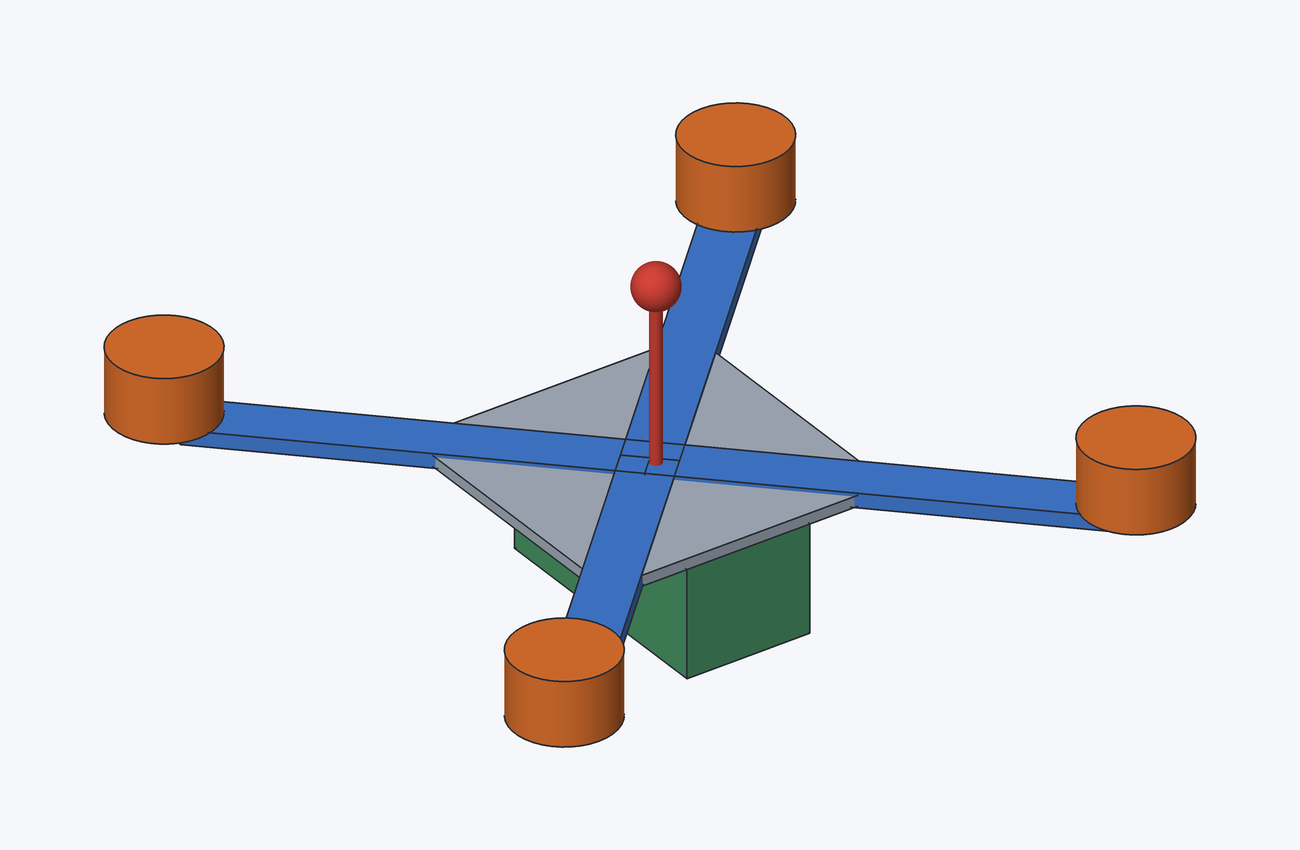
\includegraphics[width=0.55\linewidth]{fig/mass_cg.png}
\caption{Quad X-frame: carbon plate and arms from density (1.6\,g/cm$^3$), four 32\,g motors and a 190\,g
battery as COTS overrides. The battery is mounted 5\,mm forward, which puts the CG (red plumb line and
marker) at $x=2.45$\,mm. That is exactly what the balance check in \eref{ROB-04} must flag.
Computed in headless FreeCAD.}
\label{fig:cg}
\end{figure}

\begin{epic}{ROB-04}{Drone balance \& thrust-to-weight}{M3}{\stTodo}{FCB-P2R-08}
Compare the CG with the centroid of the motor axes, and report thrust-to-weight
$T/W=\sum_i T_{\max,i}/(m g)$ from COTS data. Warn when the horizontal CG offset exceeds a fraction of the
arm length, or $T/W<2$.
\emph{Acceptance:} the check flags the offset battery in Figure~\ref{fig:cg}.
\end{epic}

\begin{epic}{ROB-05}{Kinematic chains \& joint drive}{M5}{\stTodo}{FCB-P2A-09/10}
Build a link chain from revolute joints, show a joint table, read out end-effector forward kinematics, drive
the chain from the table through the stock Simulation (servo-sweep presets), and export video.
\emph{Acceptance:} the 2-DOF arm's FK matches a hand calculation.
\end{epic}

\paragraph{Theory: forward kinematics.} Each joint $i$ contributes a homogeneous transform
$T_i(\theta_i)=\begin{pmatrix}R(\mathbf a_i,\theta_i)&\mathbf p_i-R(\mathbf a_i,\theta_i)\mathbf p_i\\
\mathbf 0^{\!\top}&1\end{pmatrix}$, a rotation about its axis through $\mathbf p_i$ in the reference pose.
The end-effector pose is the product
\[
  T_{\text{ee}}(\boldsymbol\theta)=T_1(\theta_1)\,T_2(\theta_2)\cdots T_n(\theta_n)\,T_{\text{ee}}(\mathbf 0),
\]
the product-of-exponentials form, which needs no Denavit--Hartenberg frames and can be read directly from the
assembly's joints. For the planar 2-DOF arm, this reduces to
$x=\ell_1\cos\theta_1+\ell_2\cos(\theta_1+\theta_2)$ and $y=\ell_1\sin\theta_1+\ell_2\sin(\theta_1+\theta_2)$,
the acceptance check.

%======================================================================
\section{Track ECD --- ECAD bridge (KiCad)}\label{sec:ecd}
%======================================================================

\begin{epic}{ECD-01}{ECAD intake \& adopt-vs-build}{M1}{\stTodo}{FCB-P2E-01..04}
Requirements intake from the ECAD owner (KiCad version, outline and keep-outs, direction of placement sync,
STEP needs, sample board). Evaluate the KiCad StepUp add-on on current FreeCAD with a KiCad 9 board,
including its AGPL licence and maintenance. Then a decision memo: adopt StepUp unmodified, or build a bridge on
\code{kicad-cli} and the KiCad 9 IPC API. The Ops sample data shows this gate as done, but the result isn't
recorded (open question).
\end{epic}

\begin{epic}{ECD-02}{Board STEP into assembly}{M3}{\stTodo}{FCB-P2E-05}
Export with \code{kicad-cli pcb export step}, and insert into the assembly with an LCS at the board origin, so
the board joints like any component.
\end{epic}

\begin{epic}{ECD-03}{Board outline round-trip}{M3}{\stTodo}{FCB-P2E-06, P2E-09}
Pull \code{Edge.Cuts} into a Sketcher sketch and push edits back to \code{.kicad\_pcb}.
\emph{Acceptance:} the round-trip outline delta is below 0.01\,mm on the sample board.
\end{epic}

\begin{epic}{ECD-04}{Placement sync \& enclosure fit}{M3}{\stTodo}{FCB-P2E-07/08}
Push connector and mounting-hole positions from MCAD to ECAD and back. Check board against housing with the
interference command (\eref{ASM-06}).
\emph{Acceptance:} the fit check flags a connector moved into a wall.
\end{epic}

%======================================================================
\section{Track WIR --- Wire routing}\label{sec:wir}
%======================================================================

Servo arms, quad power leads and board-to-ESC runs need a wire that can be seen, measured and moved with
the joint. Fusion~360 has no harness product. This track is SolidWorks electrical-routing parity plus that
robotics need. It sits on M3 and M5, after joints exist (\eref{ASM-03}), and it stays off the M1 path that
models \code{LE-02001}.

The tube is ordinary FreeCAD. \code{Part.Wire.makePipeShell} sweeps a circle along a centerline, and
Draft's \code{filletWire} rounds every corner of a polyline to an exact radius. The centerline is that
polyline: a straight lead-out along the port's local $+Z$, then the clips, with each corner filleted.
The fillet radius is the minimum bend radius, and the centerline length is the cut length. Fillets hold
that minimum exactly, which a free B-spline cannot. BIM pipes are the same sweep at building scale and are
tied to IFC; they do not follow assembly links. The wire is its own \code{Part::FeaturePython}.

A port is an \code{App::LocalCoordinateSystem}, the same kind of datum as the mounting LCS in
\eref{ROB-01}. End placements come from \code{UtilsAssembly.getGlobalPlacement}, which already resolves a
link chain through \code{getPlacementOf}. A datum stays put when the model is edited; a face pick does not.
When \eref{WIR-02} starts, the add-on lives at \file{package/bruceworx/mods/WireRouting/}, installed the
same way as the History Timeline. Python only, no C++.

Following a joint is the part that takes care. The wire lives in the assembly, both ends are ports on
links, and a recompute after the solver moves a link rebuilds the centerline. Bundles are a small graph:
several wires share a sleeve, then break out. Clip-graph routing is a shortest path through clips the user
already placed, keeping a segment only when its fillet succeeds. Two commercial features stay off this
track: free-space auto-route through an obstacle mesh, and a flattened nailboard drawing. A fillet that
cannot be built is the bend-radius check. Clearance of the finished solid can later reuse
\eref{ASM-06}.

\eref{WIR-01} is a short adopt-versus-build spike, the same shape as \eref{ECD-01}. Try the community
Cables workbench on an assembly with two moving links, then write the decision down. Those add-ons route
inside one document. The spike is there so a workbench that cannot follow an \code{Assembly} joint is not
vendored. The expected result is to build.

\begin{epic}{WIR-01}{Adopt versus build}{M3}{\stTodo}{(new)}
Try the community Cables workbench on an assembly with two moving links. Record the decision: adopt it
unmodified, or build the Python add-on described above.
\emph{Acceptance:} the decision memo is written.
\end{epic}

\begin{epic}{WIR-02}{Port and wire}{M3}{\stTodo}{(new)}
A port datum, a straight lead-out along local $+Z$, \code{filletWire} at the minimum bend radius, a circle
swept with \code{makePipeShell}, and a read-only length.
\emph{Acceptance:} a three-corner wire matches the analytic line-plus-arc length within 0.01\,mm. A corner
tighter than the radius fails the check and produces no solid.
\end{epic}

\begin{epic}{WIR-03}{Assembly follow}{M3}{\stTodo}{(new)}
The wire lives in the assembly. Both ends are ports on links, and a recompute after the solver moves a
link rebuilds the centerline. Depends on \eref{WIR-02} and \eref{ASM-03}.
\emph{Acceptance:} dragging a revolute joint updates the length, and both ends stay on their ports.
\end{epic}

\begin{epic}{WIR-04}{From-to cut list}{M3}{\stTodo}{(new)}
Gauge, color, from, to and length for each wire. The assembly BOM (\eref{ASM-04}) carries the same rows.
\emph{Acceptance:} the cut list matches the wire lengths, and the BOM carries the rows.
\end{epic}

\begin{epic}{WIR-05}{Clips and bundles}{M5}{\stTodo}{(new)}
Clips are waypoints. A bundle is a shared sleeve with a breakout: several wires share a middle segment,
then split to their own ports. Depends on \eref{WIR-03}.
\emph{Acceptance:} two wires share one middle segment and split to two ports; the sleeve length is that
segment.
\end{epic}

\begin{epic}{WIR-06}{Route on the clip graph}{M5}{\stTodo}{(new)}
A from-to list becomes a shortest feasible path through clips the user placed. A segment is feasible when
its fillet succeeds. Board pins become ports only after \eref{ECD-04}; this epic does not wait on that.
\emph{Acceptance:} a three-clip fixture picks the shorter feasible path and reports its length.
\end{epic}

%======================================================================
\section{Track AUT --- AI and automation}\label{sec:aut}
%======================================================================

\begin{epic}{AUT-01}{Headless hooks \& CLI}{M0}{\stDone}{FCB-P2-11..14}
Merged in \#5: \file{addons/BruceWorx/hooks.py} exports STEP, lists the document tree as JSON, and
numbers and renames parts through FreeCADCmd. Every later automation epic builds on it.
\end{epic}

\begin{epic}{AUT-02}{bruceworx.api}{M1}{\stTodo}{FCB-P2AI-03}
A stable Python module over the hooks: create and edit parts, set parameters (\eref{MOD-02}), read the tree,
export STEP/STL/3MF, run inspections (\eref{MOD-11}). One undo transaction per call.
\emph{Acceptance:} the API is covered by headless tests in CI.
\end{epic}

\begin{epic}{AUT-03}{MCP server}{M1}{\stTodo}{FCB-P2AI-01/02, 04..08}
Choose a base among the MIT and LGPL FreeCAD MCP servers (spike plus gate, including whether raw
\code{execute\_code} is allowed), then add BruceWorx tools: tree, create/edit, export, numbering, COTS
insert, mass report. Includes a headless mode on FreeCADCmd for cloud agents, and security: localhost by
default, a token, and an audit log. Configuration docs for the agents in use, and integration tests in CI.
\emph{Acceptance:} an agent creates, queries and exports a part headless in CI.
\end{epic}

\begin{epic}{AUT-04}{Assistant panel}{M5}{\stTodo}{FCB-P2AI-09..15}
A dock with chat, a tool-call preview, and apply/undo per action. It calls \code{bruceworx.api} and MCP, and
gets a UX mock and design gate first.
\emph{Acceptance:} a try-out on real CAD work is signed off.
\end{epic}

\begin{epic}{AUT-05}{Command line}{M5}{\stTodo}{(new, from the UI plan)}
A bottom command line accepting AutoCAD-style aliases, inline Python, CadQuery/build123d scripts and
OpenSCAD, plus a \code{CodeFeature} that keeps a script as a parametric, trust-gated feature.
\emph{Acceptance:} \code{CPATTERN @Bolt Q 8} reproduces Figure~\ref{fig:examples}d, and a build123d box lands
as a solid in the timeline.
\end{epic}

\begin{figure}[ht]
\centering
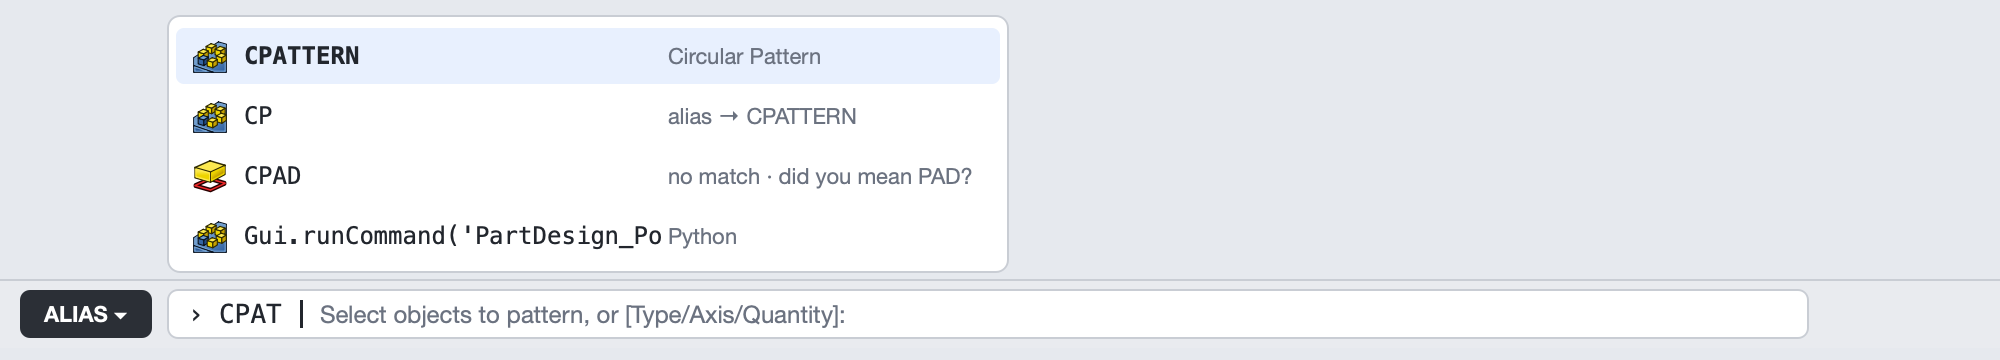
\includegraphics[width=\linewidth]{fig/cmdline.png}
\caption{Command line typing \code{CPAT} (working mock): ranked completions, the alias expansion, a ``did
you mean'' suggestion and the Python equivalent, with an AutoCAD-style \texttt{[Option/Option]} prompt.}
\end{figure}

\begin{figure}[ht]
\centering
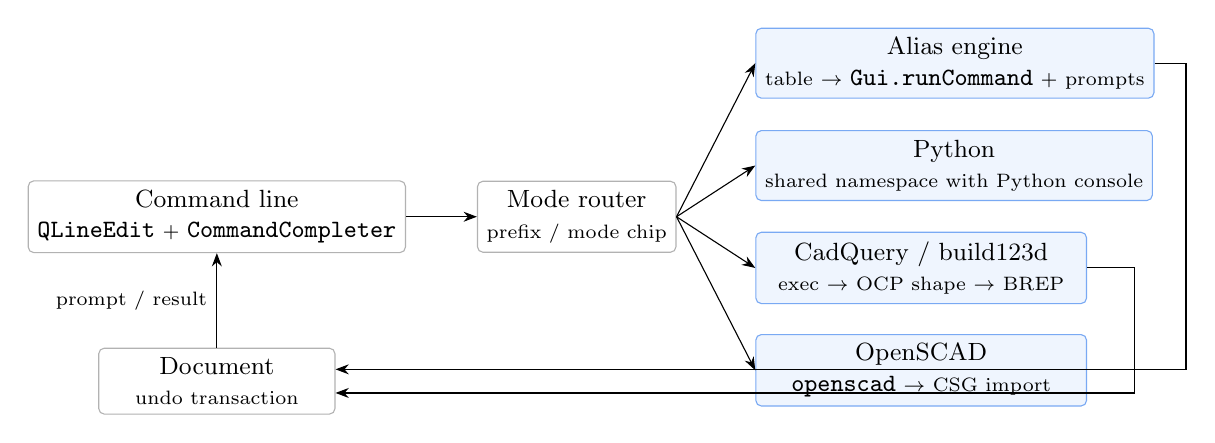
\begin{tikzpicture}[>=Stealth,
  b/.style={draw=black!30,rounded corners=2pt,fill=white,minimum height=0.8cm,align=center,font=\small},
  m/.style={b,fill=bwblue!7,draw=bwblue!60}]
\node[b,minimum width=3cm] (in) {Command line\\\scriptsize\code{QLineEdit} + \code{CommandCompleter}};
\node[b,right=0.9cm of in,minimum width=2.4cm] (r) {Mode router\\\scriptsize prefix / mode chip};
\node[m,right=1cm of r,yshift=1.95cm,minimum width=4.2cm] (a) {Alias engine\\\scriptsize table $\to$ \code{Gui.runCommand} + prompts};
\node[m,right=1cm of r,yshift=0.65cm,minimum width=4.2cm] (p) {Python\\\scriptsize shared namespace with Python console};
\node[m,right=1cm of r,yshift=-0.65cm,minimum width=4.2cm] (c) {CadQuery / build123d\\\scriptsize exec $\to$ OCP shape $\to$ BREP};
\node[m,right=1cm of r,yshift=-1.95cm,minimum width=4.2cm] (o) {OpenSCAD\\\scriptsize \code{openscad} $\to$ CSG import};
\node[b,below=1.2cm of in,minimum width=3cm] (doc) {Document\\\scriptsize undo transaction};
\draw[->] (in) -- (r);
\foreach \x in {a,p,c,o} \draw[->] (r.east) -- (\x.west);
\draw[->] (a.east) -- ++(0.4,0) |- ($(doc.east)+(0,0.15)$);
\draw[->] (c.east) -- ++(0.6,0) |- ($(doc.east)+(0,-0.15)$);
\draw[->] (doc.north) -- node[left,font=\scriptsize]{prompt / result} (in.south);
\end{tikzpicture}
\caption{Command-line pipeline; each run is one undo transaction.}
\end{figure}

\paragraph{Design.} A bottom toolbar spanning the window, with focus key \code{:} or \code{Ctrl+`}. An
explicit mode chip (\code{ALIAS}/\code{PY}/\code{CQ}/\code{B3D}/\code{SCAD}) plus prefixes (\code{>>>},
\code{cq:}, \code{b3d:}, \code{scad:}), with alias mode as the default. Completion reuses FreeCAD's
\code{Gui::CommandCompleter}. Python runs in the console interpreter's namespace. OpenSCAD uses the
existing importer. No maintained add-on provides an AutoCAD-style line, and none bridges build123d into FreeCAD
(only the reverse, \code{ocp-freecad-cam}), so both are written here.

\paragraph{Theory: alias grammar and prompts.} Aliases live in a plain file in the spirit of AutoCAD's
\code{acad.pgp}. A line is parsed as
\begin{lstlisting}
line     := command ( WS arg )*
command  := ALIAS | COMMAND_NAME            ; case-insensitive
arg      := number unit? | option | ref
option   := IDENT                           ; matched against [A/B/C] prompt options
ref      := '@' object-label ( '.' subelement )?   ; e.g. @Flange.Face3
\end{lstlisting}
Missing arguments are asked for by a prompt state machine,
$\textsc{Select}\to\textsc{Option}^{*}\to\textsc{Value}^{*}\to\textsc{Commit}$. Viewport selection, a typed value or
Enter advances it, and Esc aborts the transaction.

\paragraph{Theory: ranking completions.} For query $q$ and candidate $c$,
\[
  \sigma(q,c) = 4\,[\,q \sqsubseteq_{\text{prefix}} c\,] + 2\,[\,q \sqsubseteq_{\text{initials}} c\,]
  + \frac{|q|}{\operatorname{span}(q,c)} + \lambda\log(1+f_c),
\]
where $\operatorname{span}$ is the shortest window of $c$ containing $q$ as a subsequence and $f_c$ is the
user's usage count. Unknown input gets the smallest Damerau--Levenshtein candidate (``did you mean PAD?'').

\paragraph{Theory: code-CAD bridge.} CadQuery and build123d wrap OCCT through OCP (pybind11), and FreeCAD
through \code{TopoShape}. Even when both load the same OCCT libraries, passing raw \code{TopoDS\_Shape}
pointers would couple two binding ABIs. The bridge therefore serialises through OCCT's BREP format:
$\texttt{OCP shape}\xrightarrow{\texttt{BRepTools::Write}}\text{BREP}\xrightarrow{\texttt{importBrepFromString}}\texttt{TopoShape}$.
Measured on the flange (15 faces, 10.9\,kB): 0.17\,ms to write and 0.12\,ms to read on the FreeCAD side,
with exact volume round-trip. The OCP-side write is still to be measured \verify.
\code{CodeFeature}s re-execute on recompute, so they start \emph{untrusted}, with recompute disabled until
the user approves them, the same trust model as FreeCAD macros.

\paragraph{Dependencies and the upstream-main decision.}
\begin{center}
\small
\begin{tabularx}{\linewidth}{@{}lllX@{}}
\toprule
Package (conda-forge) & Version & Needs & Fit with the current build (OCCT 7.8.1, Python 3.11)\\
\midrule
\code{ocp} & 7.8.1.2 & occt 7.8.1 \code{all\_h869bdd7\_203} & Same OCCT build hash as \file{pixi.lock} (osx-arm64)\\
\code{build123d} & 0.9.1 & ocp $\ge$7.8,$<$7.9 & OK\\
\code{cadquery} & 2.7.0 & ocp $\ge$7.8.1,$<$7.9 & OK, pin \code{<2.8}\\
\code{cadquery} & 2.8.0 & ocp 7.9.3.1 & Conflicts with OCCT 7.8\\
\code{openscad} & --- & --- & Not on conda-forge; separate binary\\
\bottomrule
\end{tabularx}
\end{center}
Tracking upstream main (\eref{FND-03}) means FreeCAD's OCCT will move to 7.9 or later. The OCP pin must then
move with it: CadQuery 2.8 already pairs with OCP 7.9.3. The pin is re-solved whenever the nightly
rebase changes \code{occt} in \file{pixi.toml}, and the command line's code-CAD modes are disabled with a
message, never broken, if no matching OCP exists yet.

%======================================================================
\section{Track UIX --- UI and styling (after M2)}\label{sec:uix}
%======================================================================

Styling comes after the functional tracks, as decided. Three epics are already merged or under way: the
preference pack and viewport styling (\#8), the macOS title bar and overlay tree (\#6), and the timeline
spike (\#7). The rest of this chapter is the Fusion-style layout from the earlier UI plan, kept as the
\emph{starting brief} for the redesign. Its mocks are redrawn in \eref{UIX-09}; the first round is section~\ref{sec:ui-design}.

\begin{epic}{UIX-01}{Theme, pref pack \& viewport styling}{UI}{\stDone}{FCB-P1-01..05, P1V-01..07, P1V-10..18}
Merged (\#8). Follow-ups: the anti-aliasing check on Retina, and the mechanical user's try-out and sign-off.
\end{epic}
\begin{epic}{UIX-02}{macOS title bar}{UI}{\stDone}{FCB-P1F-01..05, P1F-26}
Merged (\#6): unified title bar and native window buttons behind a preference.
\end{epic}
\begin{epic}{UIX-03}{Browser (overlay model tree)}{UI}{\stProg}{FCB-P1F-06..14, P1F-27}
Prefs/QSS version merged (\#6). The free-floating panel (any inset, free height) needs a small
\code{OverlayManager} patch (FCB-P1F-11). Also fix it not showing on first run (\eref{FND-06}).
\end{epic}
\begin{epic}{UIX-04}{History timeline}{UI}{\stProg}{FCB-P1F-15..25, P1F-28}
Spike and mock merged (\#7). Remaining: the full bar with marker drag, edit, suppress and reorder (where
feasible), one-row layout, playback buttons, and a path into core.
\end{epic}
\begin{epic}{UIX-05}{Workspaces \& tabs (Fusion naming)}{UI}{\stTodo}{(new, from the UI plan)}
Design / Simulation / Manufacture / Drawing workspaces; Design tabs Solid, Surface, Mesh, Sheet Metal and
Utilities, plus a contextual Sketch tab. Extra workbenches are toggled in Preferences.
\end{epic}
\begin{epic}{UIX-06}{Toolbar \& panels}{UI}{\stTodo}{(new, from the UI plan)}
Captioned tool groups at one icon size, a floating command dialog, document tabs on top, and a one-row timeline.
\end{epic}
\begin{epic}{UIX-07}{Task panel polish}{UI}{\stTodo}{FCB-P1-06/07/08}
Sketcher, PartDesign and TechDraw dialogs.
\end{epic}
\begin{epic}{UIX-08}{Matcap shading}{UI}{\stTodo}{FCB-P1V-08/09/13/14/15}
A matcap draw style behind a preference; with the preference off, rendering is stock.
\end{epic}
\begin{epic}{UIX-09}{Fresh UI design \& re-render figures}{UI}{\stTodo}{(new)}
A new visual design for the whole application, then regenerate every figure in this document with the scripts
in \file{scripts/}.
\end{epic}

\subsection{Starting brief: review of the current window}

\begin{figure}[ht]
\centering
\begin{tikzpicture}
  \node[anchor=south west,inner sep=0] (img) at (0,0) {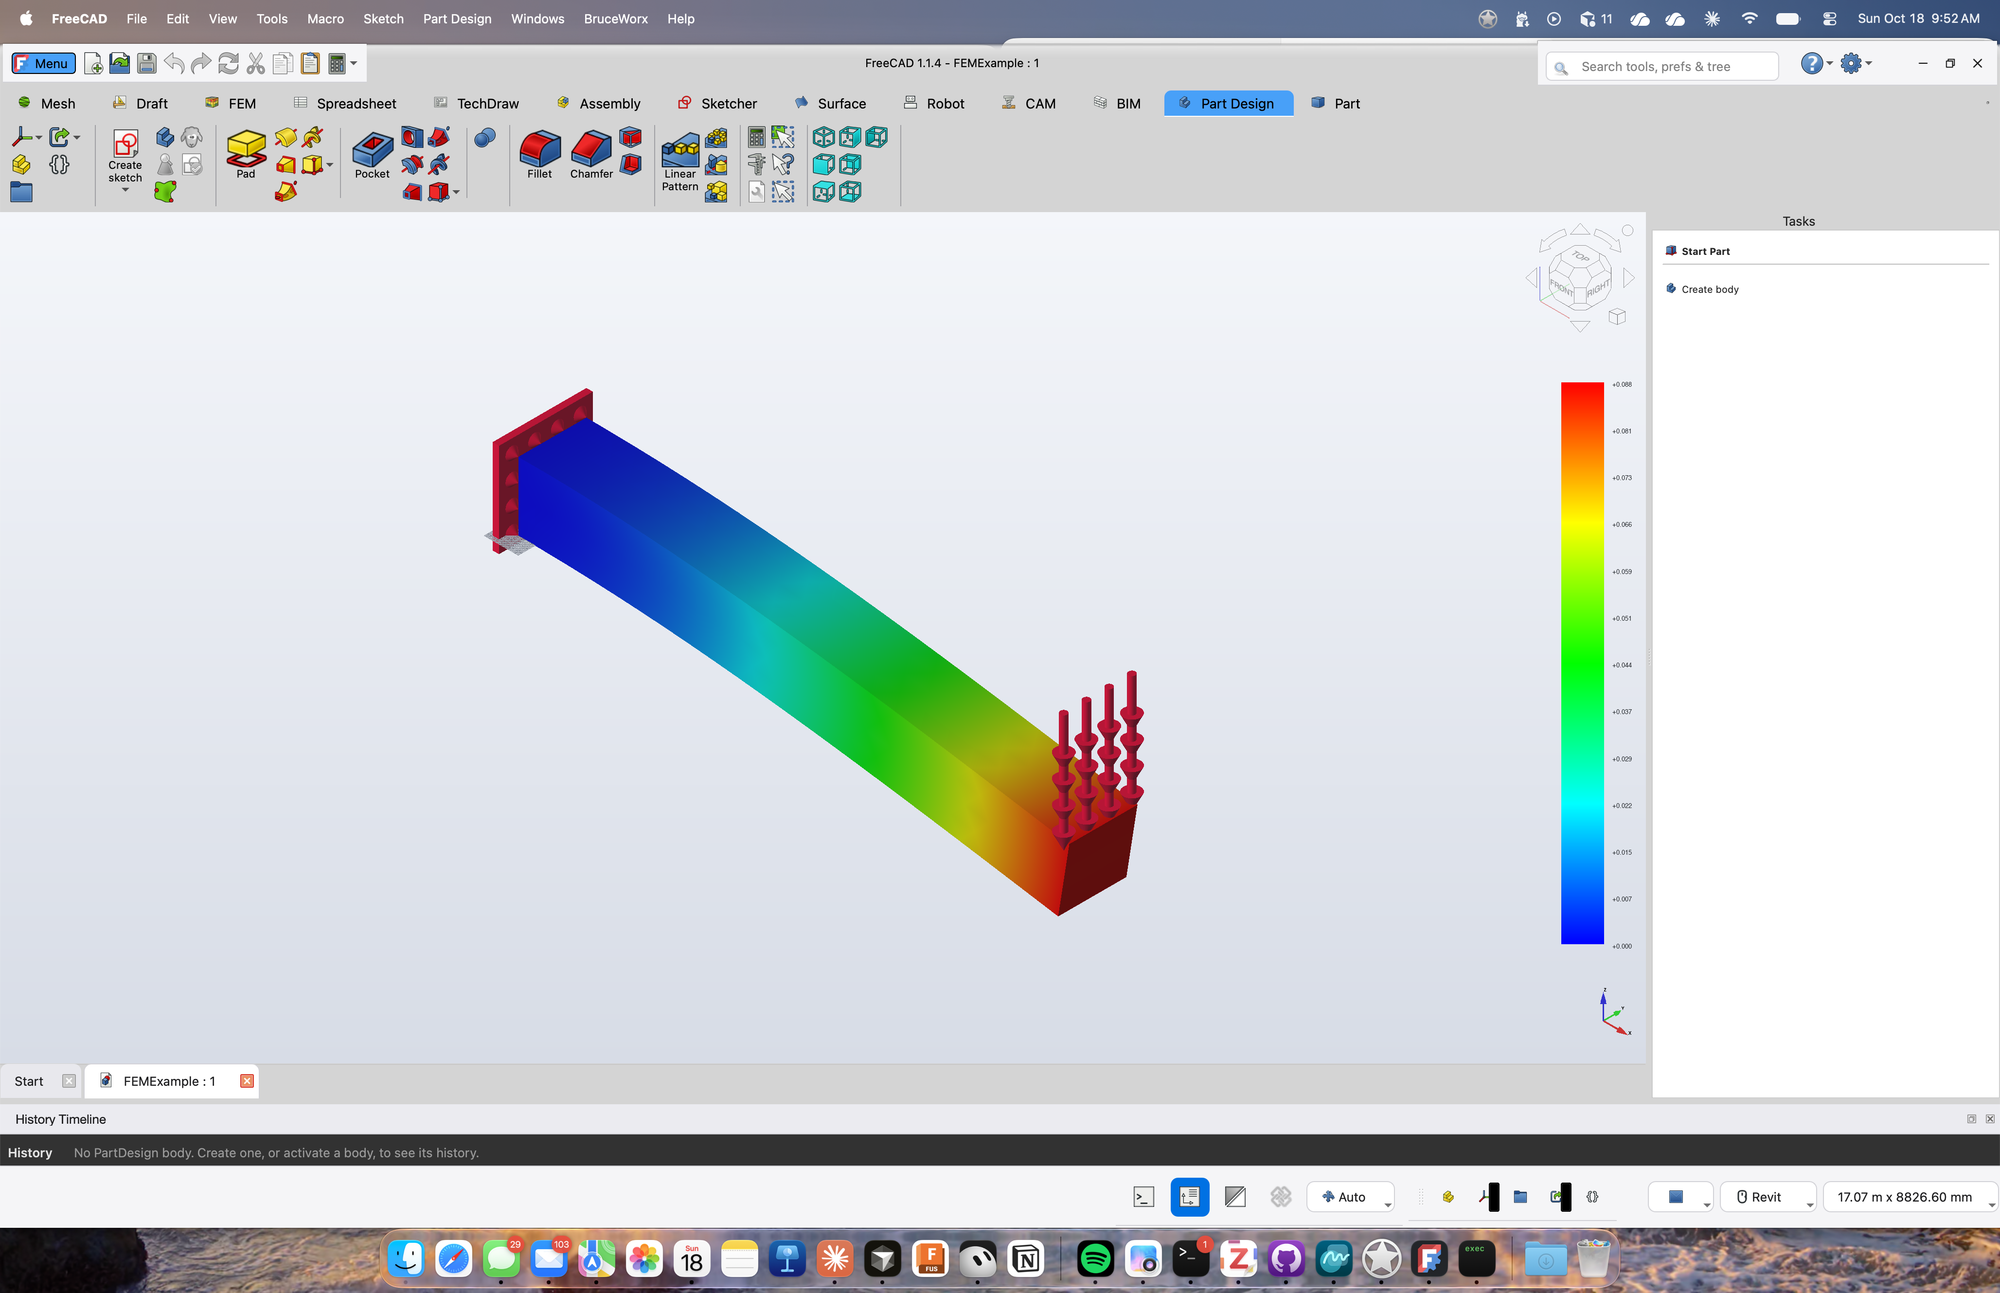
\includegraphics[width=\linewidth]{fig/before.png}};
  \begin{scope}[x={(img.south east)},y={(img.north west)}]
    \foreach \n/\x/\y in {1/0.36/0.92, 2/0.23/0.87, 3/0.90/0.77, 4/0.07/0.73, 5/0.17/0.165, 6/0.29/0.11, 7/0.53/0.075}
      \node[circle,fill=bwred,text=white,font=\scriptsize\bfseries,inner sep=1.2pt,minimum size=13pt,draw=white,line width=0.8pt] at (\x,\y) {\n};
  \end{scope}
\end{tikzpicture}
\caption{The window as of 18 Oct 2026, with issues numbered.}
\label{fig:before}
\end{figure}

\begin{center}
\small
\begin{tabularx}{\linewidth}{@{}cXX@{}}
\toprule
\# & Issue & Cause / fix\\
\midrule
\marker{1} & 13 workbench tabs & Pack trim not applied (\eref{FND-06}); replaced by workspaces (\eref{UIX-05})\\
\marker{2} & Icon grid in mixed sizes, few labels & Captioned groups, one size (\eref{UIX-06})\\
\marker{3} & Full-height Tasks column & Floating command dialog (\eref{UIX-06})\\
\marker{4} & No model tree & Overlay tree not shown (\eref{FND-06}, \eref{UIX-03})\\
\marker{5} & Document tabs at the bottom & Hard-coded \code{South} at \file{MainWindow.cpp:397}; make it a preference\\
\marker{6} & Timeline has two headers & Dock title + bar header; one 40\,px row (\eref{UIX-04})\\
\marker{7} & Crowded status bar & Readouts move beside the command line (\eref{AUT-05})\\
\bottomrule
\end{tabularx}
\end{center}

\subsection{Starting brief: proposed layout}

\begin{figure}[ht]
\centering
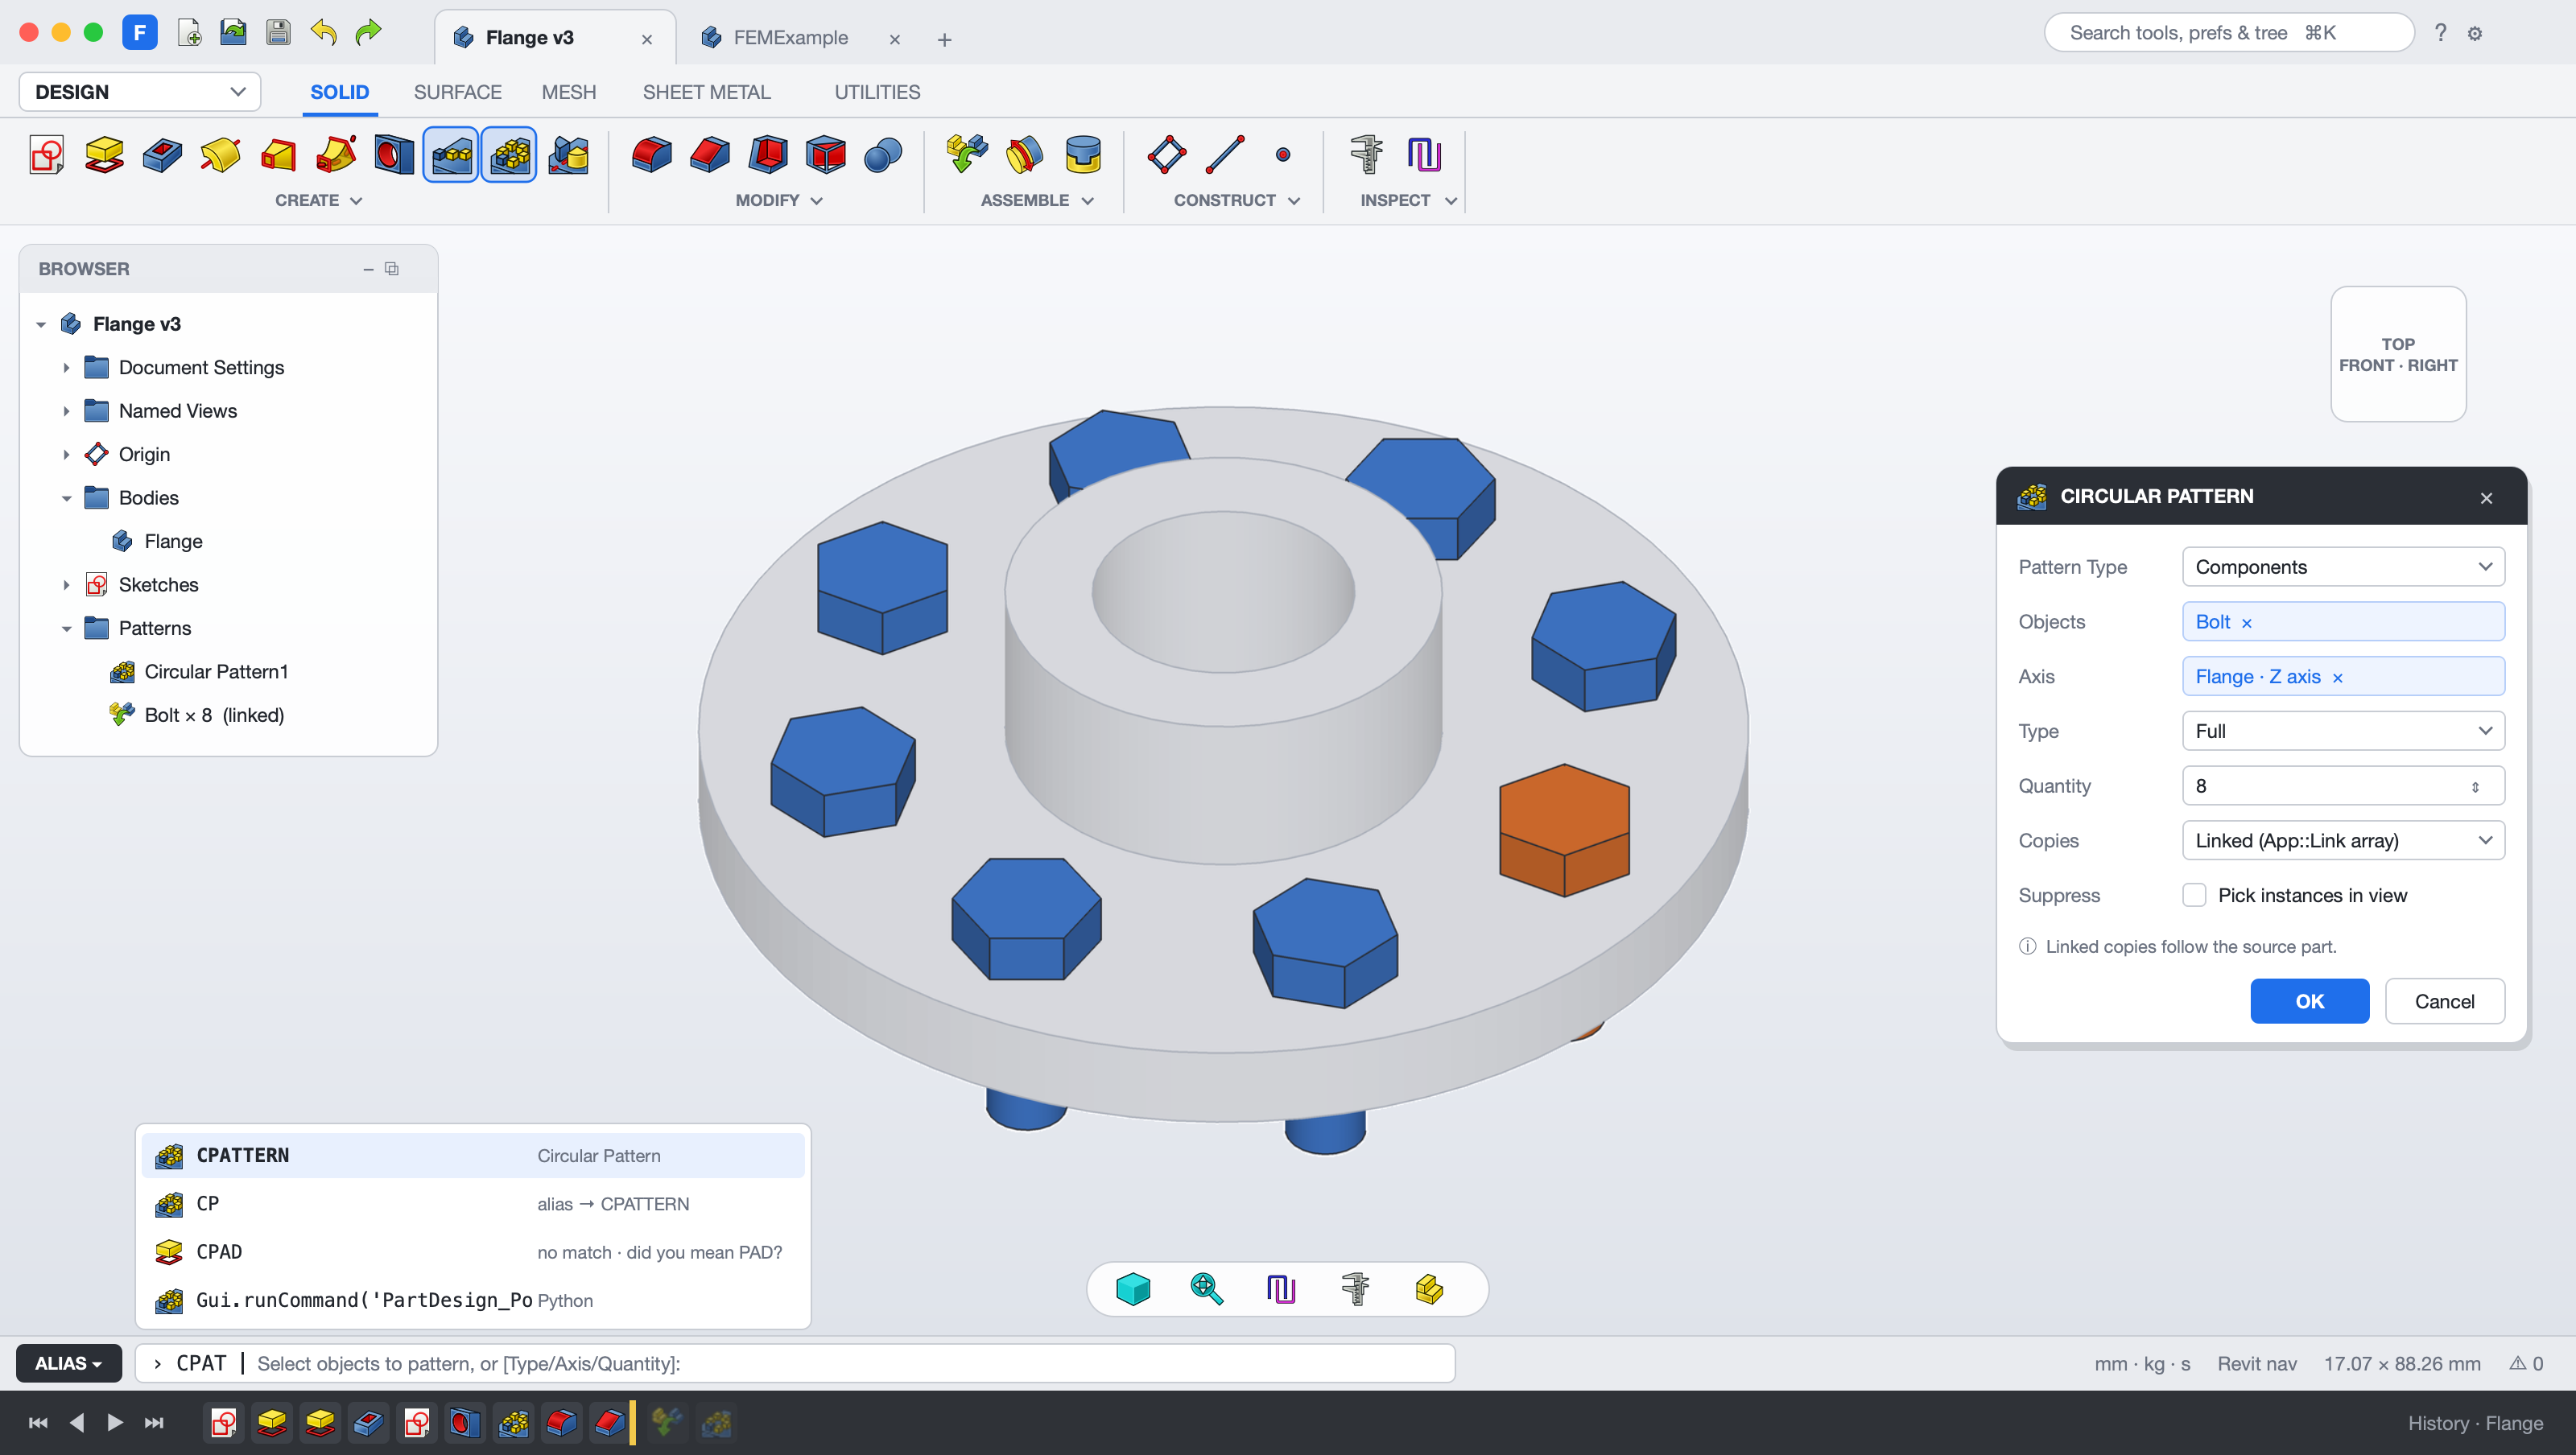
\includegraphics[width=\linewidth]{fig/layout_proposed.png}
\caption{Working mock of the Fusion-style layout: document tabs and search in the title bar; workspace
selector and tabs; captioned tool groups (Rectangular and Circular Pattern inside \textsc{Create}); Browser
top-left; floating command dialog; navigation pill; command line; timeline. FreeCAD's own icons, drawn
offscreen.}
\label{fig:after}
\end{figure}

\begin{center}
\small
\begin{tabularx}{\linewidth}{@{}llX@{}}
\toprule
Workspace & Tab & Built from\\
\midrule
\textbf{Design} & Solid & PartDesign, Part booleans, Assembly (\textsc{Assemble}), datums (\textsc{Construct}), Measure (\textsc{Inspect})\\
 & Surface & Surface workbench + Part surface tools\\
 & Mesh & Mesh and MeshPart\\
 & Sheet Metal & SheetMetal add-on (bundled)\\
 & Utilities & Spreadsheet, macros, Material, parameters (\eref{MOD-02})\\
 & \emph{Sketch} & Contextual while a sketch is open\\
\textbf{Simulation} & --- & FEM, with the study templates of \eref{SIM-01}\\
\textbf{Manufacture} & --- & CAM, print prep, flats (\S\ref{sec:mfg})\\
\textbf{Drawing} & --- & TechDraw (\S\ref{sec:drw})\\
\emph{More\ldots} & --- & Each extra workbench toggled on Preferences $\rightarrow$ BruceWorx $\rightarrow$ Workspaces\\
\bottomrule
\end{tabularx}
\end{center}

\paragraph{Selector model.} A workspace $w$ fixes a workbench $\beta(w)$, and a tab $t$ fixes a toolbar set
$\tau(w,t)$. Entering sketch edit pushes the contextual tab, and leaving pops it. Switching tabs within one
$\beta$ never switches workbench, so there is no toolbar rebuild or flicker. Implementation: a C++
\code{WorkspaceSelector} (selector type 2), a \file{workspaces.json} mapping, and a Python
\code{WorkbenchManipulator} that composes tabs from several workbenches.

%======================================================================
\subsection{UI design mock: clean but feature dense (19 Oct 2026)}\label{sec:ui-design}
%======================================================================

\textbf{Your answers (19 Oct).}
\begin{itemize}[nosep]
  \item A design mock first, then this plan, approved before any code.
  \item Light and dark, following the macOS appearance setting; the accent follows the macOS accent colour.
  \item ``Clean but feature dense.''
  \item Keep FreeCAD's icons, but at one size with consistent captions.
  \item BruceWorx's own top bar (workspace menu, tabs, captioned groups) replaces the FreeCAD-Ribbon add-on.
  \item Screens: part modelling, assembly with the joint panel, sketch, and the Start page.
\end{itemize}

The mock is HTML drawn at the size of your screen (1600$\times$1000 points, 2$\times$). It uses FreeCAD's own icons,
and its 3D views are rendered by this build. It shows what is \emph{intended}. It is not a screenshot of working
code. Every element is mapped below to how it would be built. The source is in
\file{scripts/ui\_mock/}, and \code{render.sh} redraws every figure in this section.

\subsubsection*{Where the window is today}

\begin{figure}[!htbp]
\centering
\begin{tikzpicture}
  \node[anchor=south west,inner sep=0] (img) at (0,0) {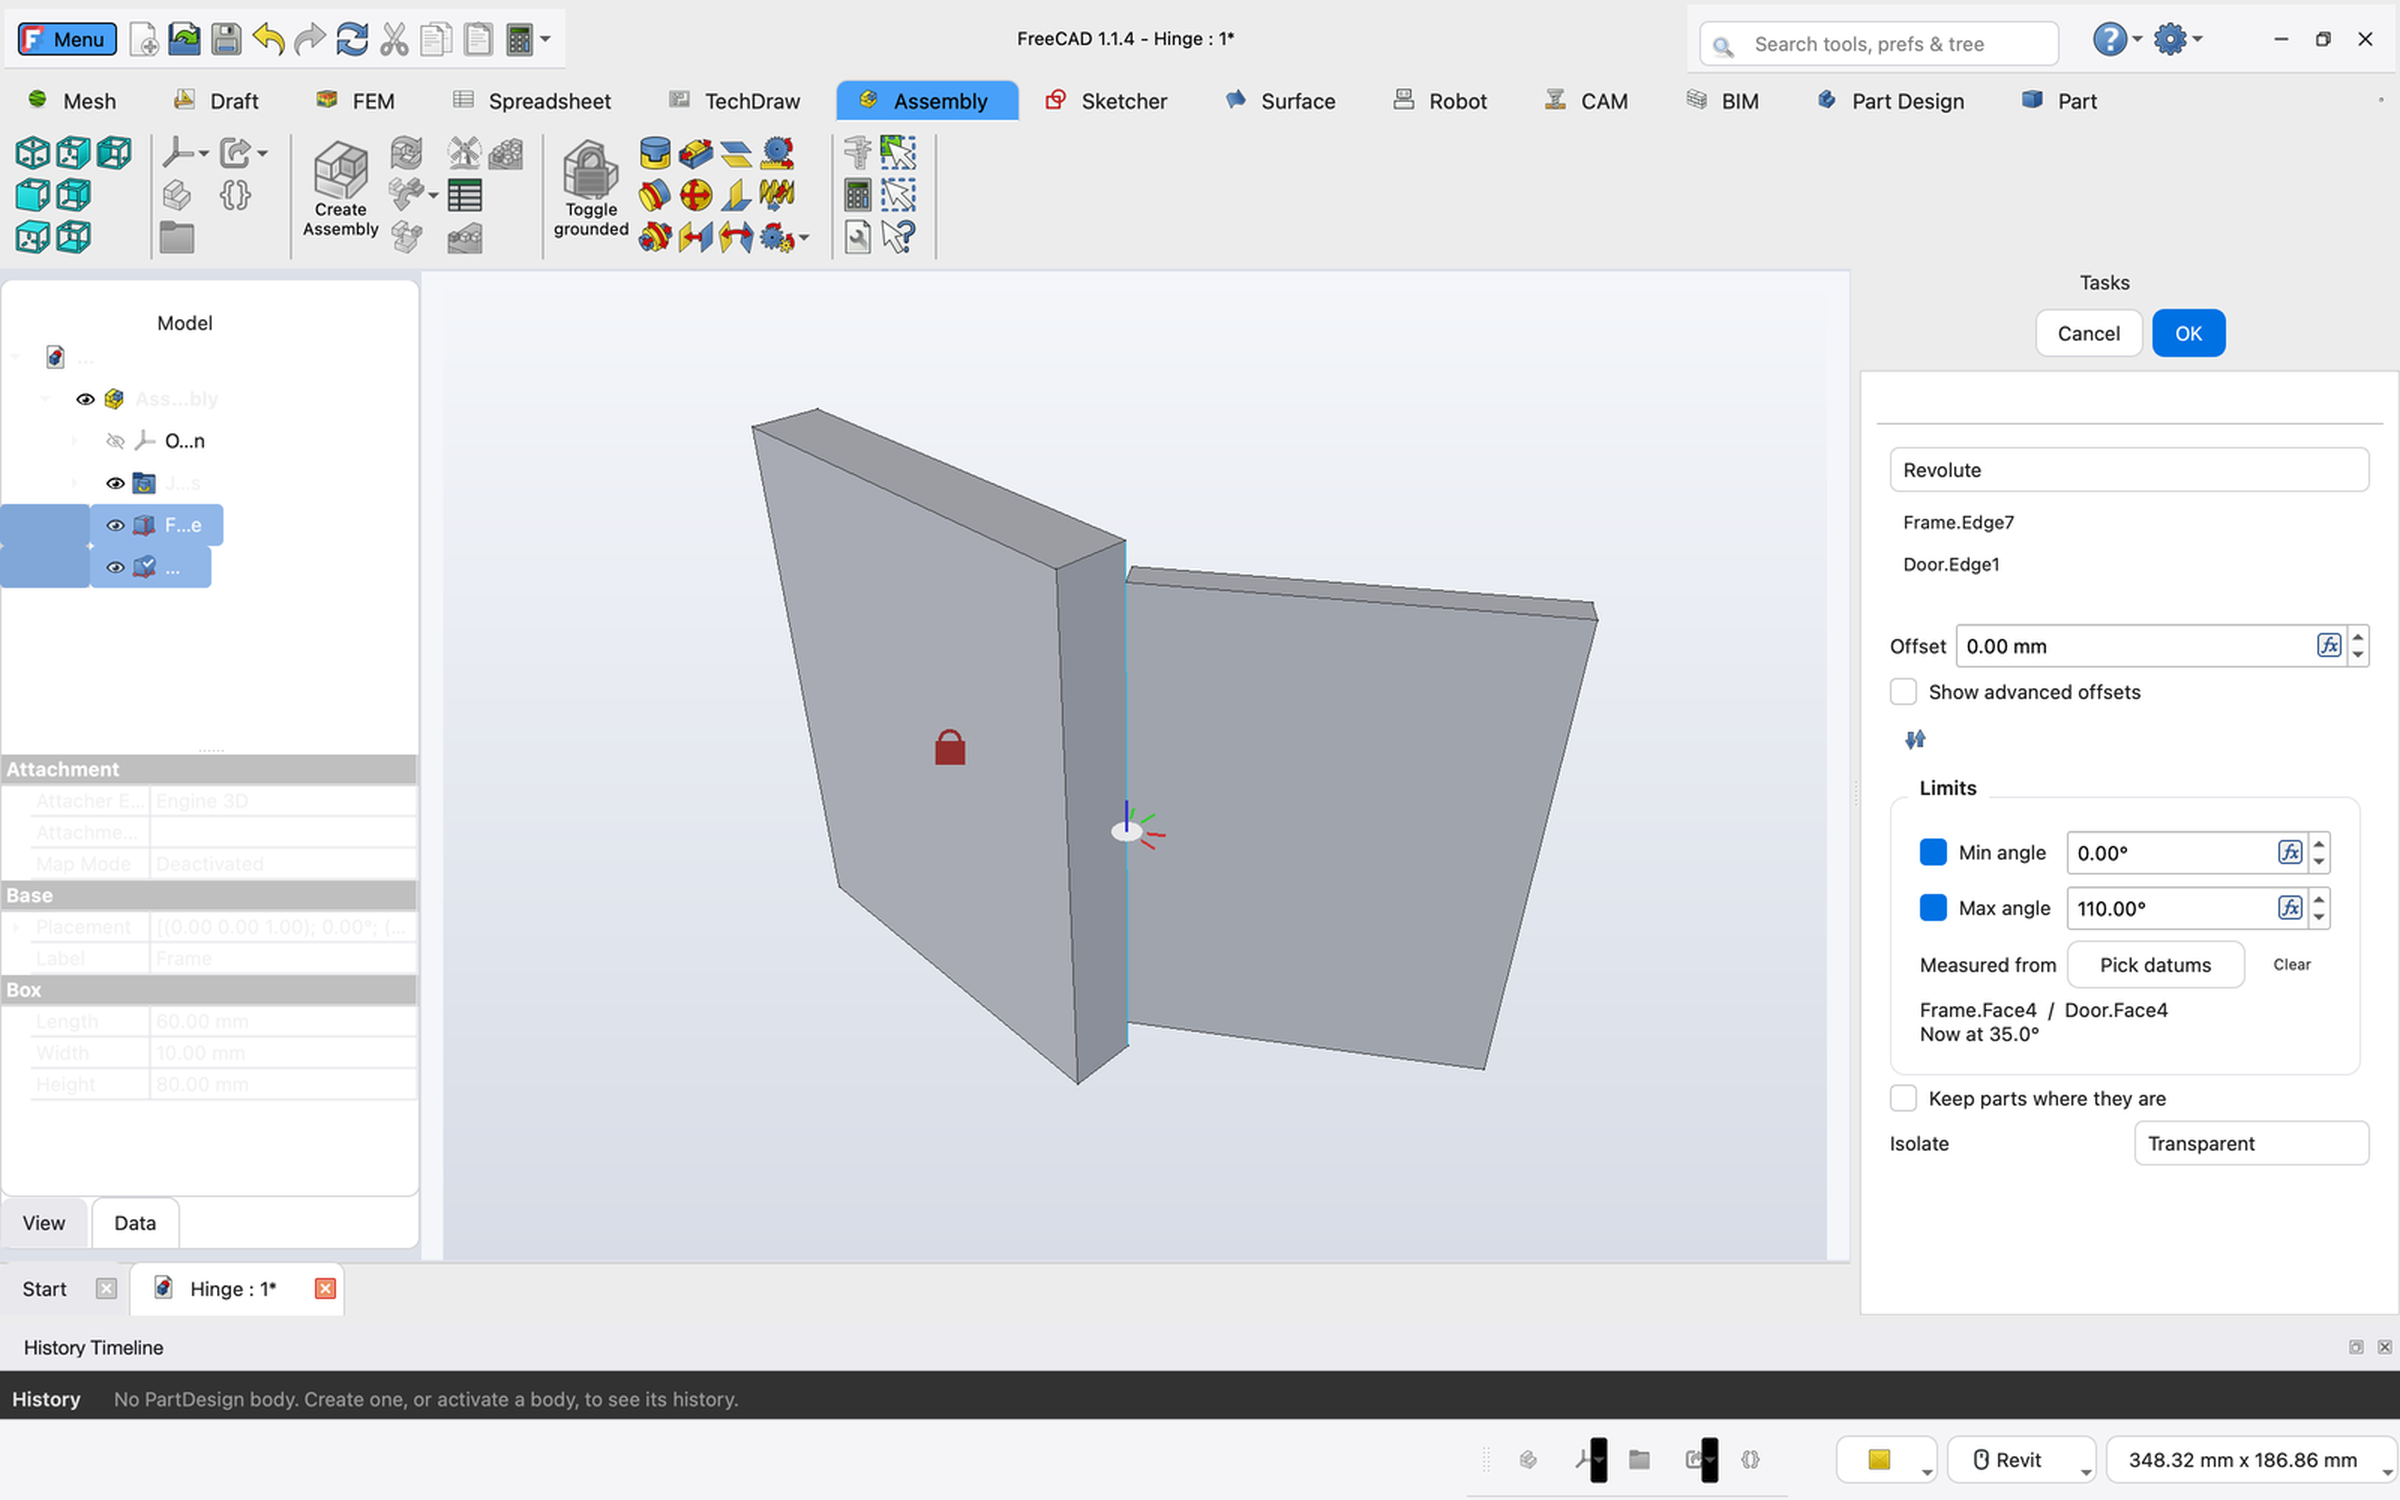
\includegraphics[width=\linewidth]{fig/ui_before_joint.png}};
  \begin{scope}[x={(img.south east)},y={(img.north west)}]
    \foreach \n/\x/\y in {1/0.035/0.972, 2/0.435/0.972, 3/0.985/0.977, 4/0.10/0.78, 5/0.175/0.53, 6/0.78/0.79, 7/0.80/0.49, 8/0.12/0.145, 9/0.05/0.105, 10/0.61/0.026}
      \node[circle,fill=bwred,text=white,font=\scriptsize\bfseries,inner sep=1.2pt,minimum size=13pt,draw=white,line width=0.8pt] at (\x,\y) {\n};
  \end{scope}
\end{tikzpicture}
\caption{This build tonight (the hinge from tests 14 and 16), with the problems numbered.}
\label{fig:ui-before}
\end{figure}

\begin{center}
\small
\begin{tabularx}{\linewidth}{@{}cXX@{}}
\toprule
\# & What you see & Cause and fix\\
\midrule
\marker{1} & ``Menu'' button, 13 workbench tabs, a large icon grid & The \textbf{FreeCAD-Ribbon} add-on (v1.12.0dev) in your FreeCAD profile, not BruceWorx. It is replaced by the BruceWorx bar; see question~3.\\
\marker{2} & Title shows ``FreeCAD 1.1.4 -- Hinge : 1*'' & Window title: the document name only, with the unsaved mark on its tab.\\
\marker{3} & Windows-style $-\,\square\,\times$ at the top right & Probably drawn by Ribbon. \verify{} Native macOS buttons (\eref{UIX-02}) come back once it is off.\\
\marker{4} & Model tree names cut short and faded (``Ass\ldots bly'', ``F\ldots e'') & The faded names have about 1.1:1 contrast. Suspected: the floating-tree sheet's white text (\file{BruceWorxModelTree.qss}) applied to a light panel, and a narrow first column. \verify\\
\marker{5} & Property headers grey on grey & Header colour from the Ribbon sheet; replaced by the token colours below.\\
\marker{6} & ``Tasks'' column the full window height, header floating & Task panel docked right. It becomes a floating command dialog with OK/Cancel at the bottom.\\
\marker{7} & Odd gaps, a stray icon, one \emph{Clear} button styled differently & Task panel layout and QSS (\eref{UIX-07}).\\
\marker{8} & Document tabs at the bottom, with red $\times$ & \code{setTabPosition(South)} is hard-coded at \file{MainWindow.cpp:397}; the red $\times$ is a stylesheet icon. \verify\\
\marker{9} & Timeline with two headers that says ``No PartDesign body'' in an assembly & Dock title plus bar header. It becomes one row and is hidden when there is no history.\\
\marker{10} & Status bar: black bars, ``Revit'', a size cut off & Status-bar widgets with no styling. \verify{} They are regrouped as quiet readouts.\\
\bottomrule
\end{tabularx}
\end{center}

\subsubsection*{The design, one screen explained}

\begin{figure}[!htbp]
\centering
\begin{tikzpicture}
  \node[anchor=south west,inner sep=0] (img) at (0,0) {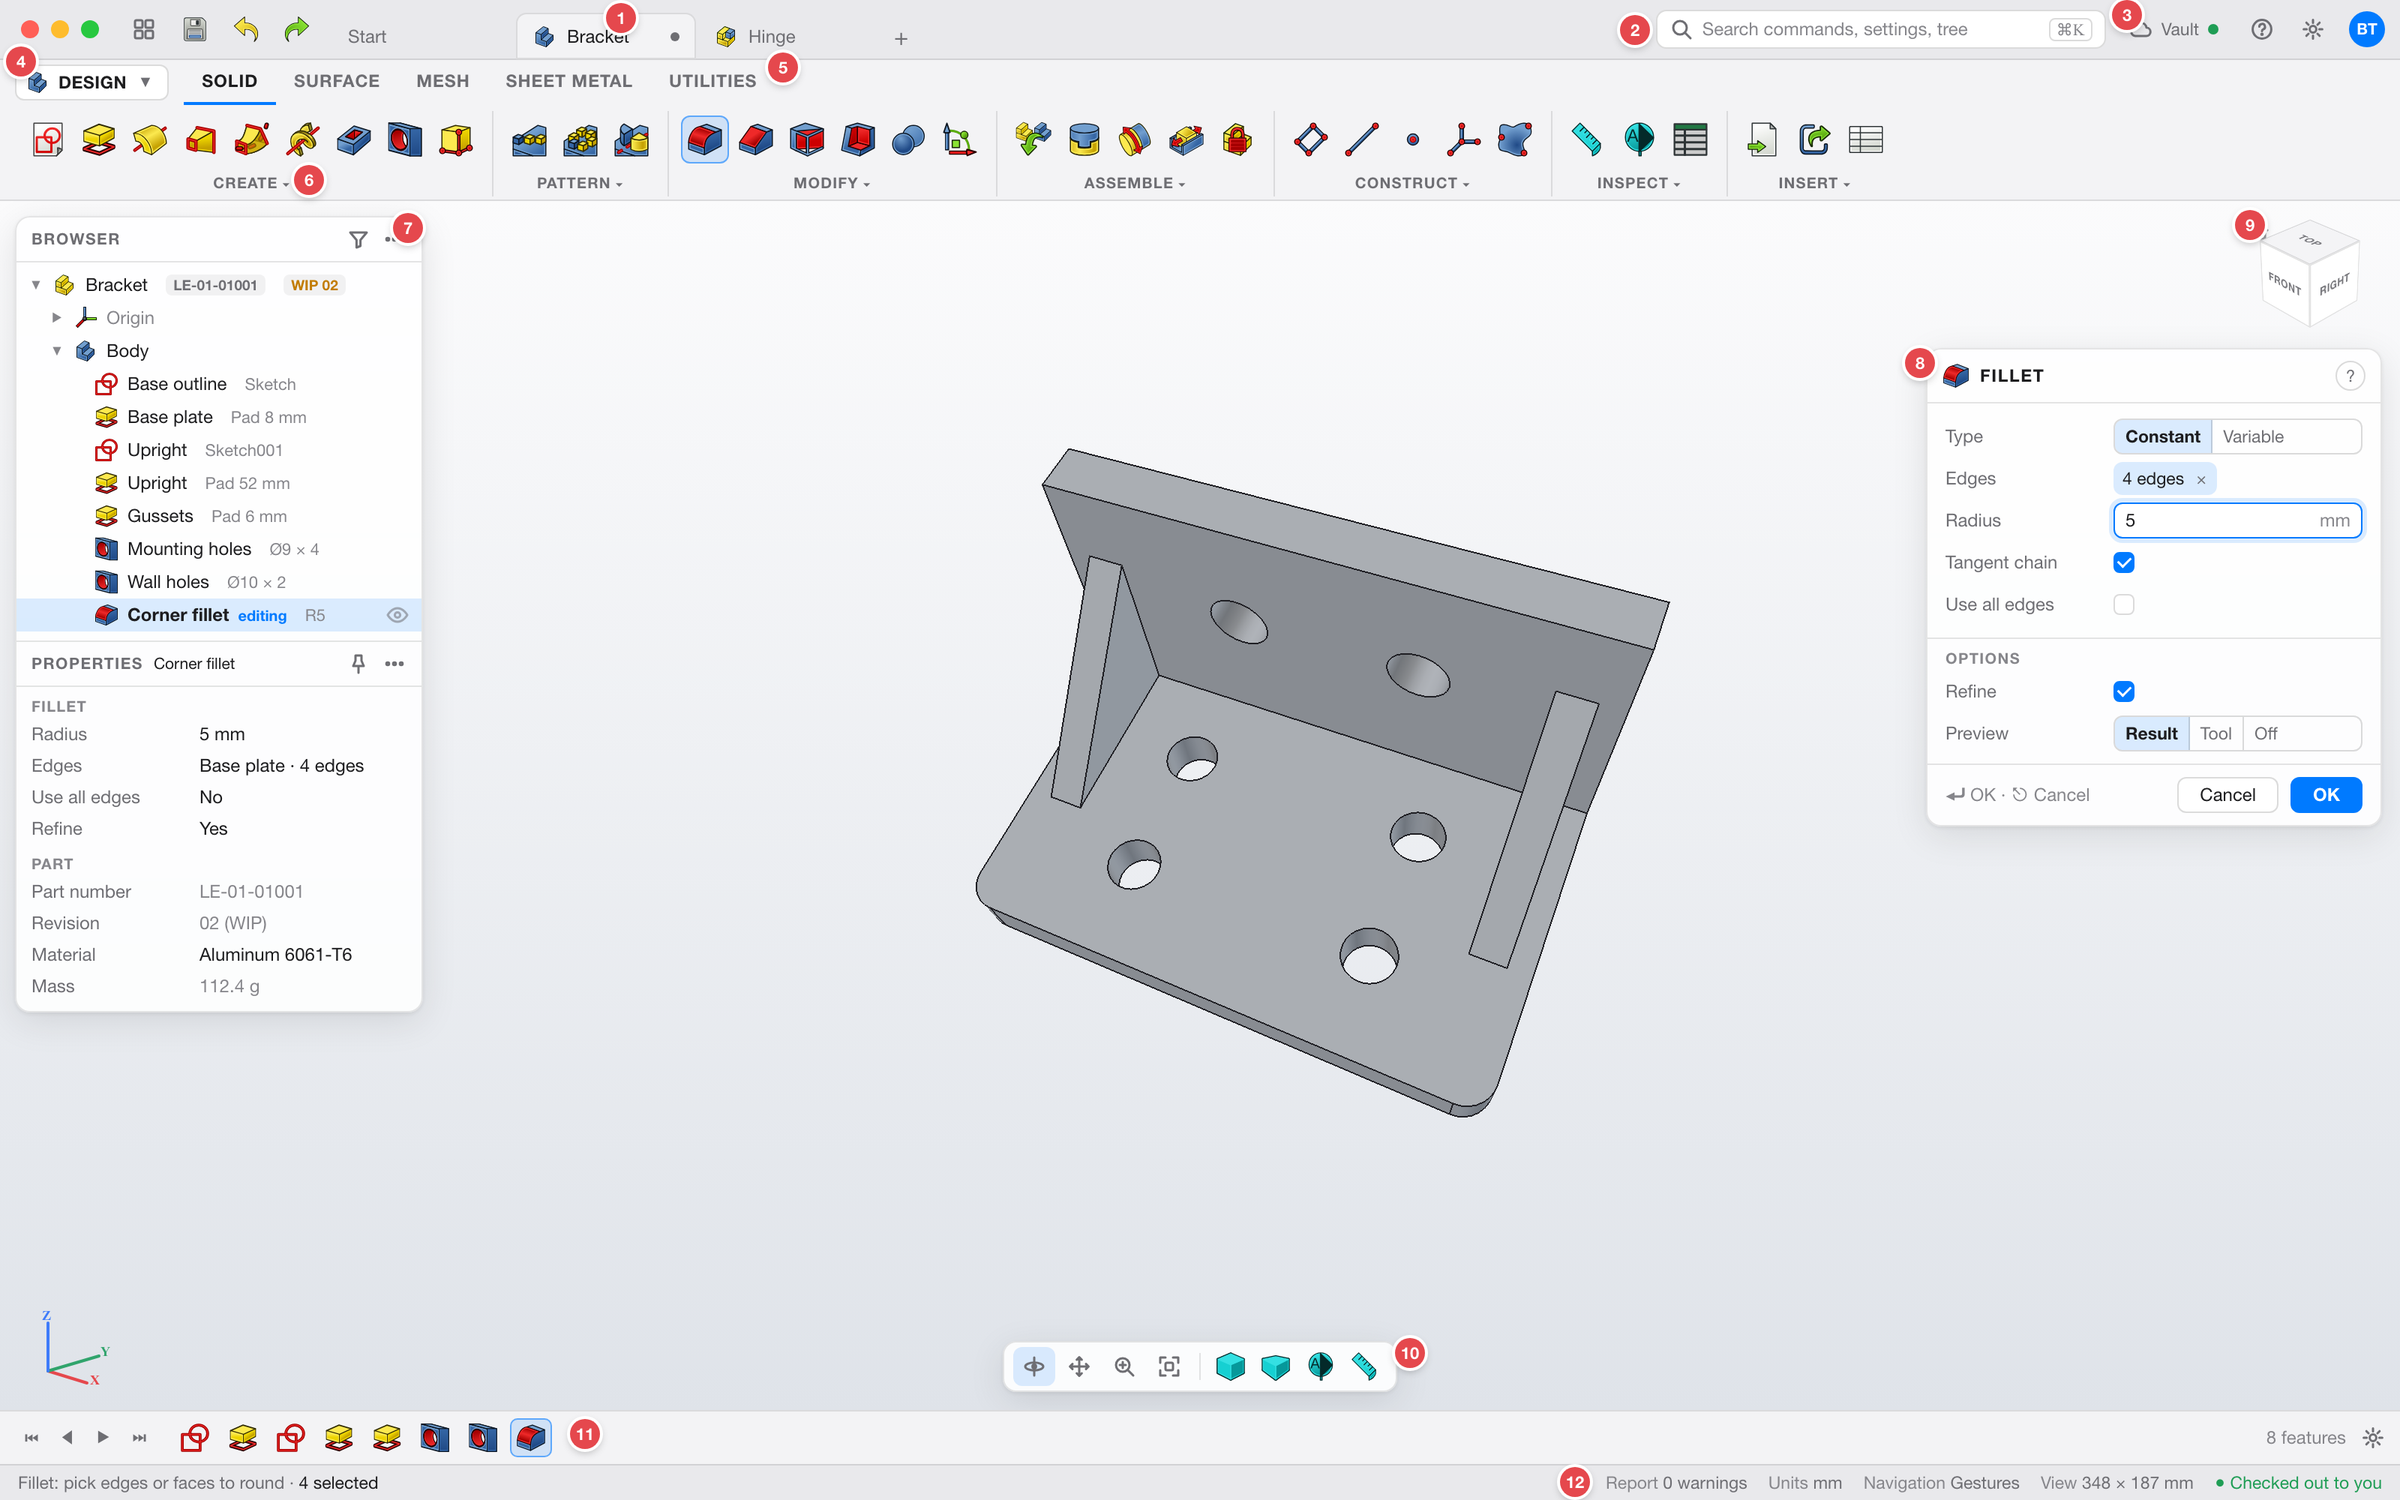
\includegraphics[width=\linewidth]{fig/ui_mock_part-notes.png}};
\end{tikzpicture}
\caption{Part modelling, light. A body with a fillet being edited. The numbers match the table below.}
\label{fig:ui-notes}
\end{figure}

\begin{center}
\small
\begin{tabularx}{\linewidth}{@{}cp{3.3cm}Xl@{}}
\toprule
\# & Element & How it is built & Epic\\
\midrule
\marker{1} & Document tabs in the title bar & Tab bar moved \code{North} (a preference instead of the hard-coded \code{South}), then hosted in the unified title bar. Modified dot instead of $\times$; $\times$ on hover. & \eref{UIX-06}\\
\marker{2} & Search, \texttt{Cmd-K} & Commands, preferences and tree in one field. Built in, or the SearchBar add-on restyled (question~2). & \eref{UIX-06}\\
\marker{3} & Vault status & Small Python status widget reading the folder vault (\S\ref{sec:pdm-eval}). & \eref{PDM-04}\\
\marker{4} & Workspace menu & \code{WorkspaceSelector}, as in the starting brief. & \eref{UIX-05}\\
\marker{5} & Tabs, plus \textsc{Sketch} in accent while a sketch is open & Toolbar sets per tab; the contextual tab is pushed on sketch edit. & \eref{UIX-05}\\
\marker{6} & Captioned groups, 24\,px icons & One icon size (preference), each toolbar given a caption and a $\blacktriangledown$ overflow menu. No icon is redrawn. & \eref{UIX-06}\\
\marker{7} & Browser with properties & Tree and property view in the left overlay as one card. Second column shows the feature summary (``Pad 8 mm''), P/N and state badges from the part properties (\S\ref{sec:partprops}). & \eref{UIX-03}\\
\marker{8} & Command dialog & Task panel in the right overlay as a card. Icon and title header, OK/Cancel at the bottom (\code{TaskDialog::South} as default), keyboard hint. & \eref{UIX-07}\\
\marker{9} & View cube & NaviCube size, colours and font are already preferences. & \eref{UIX-01}\\
\marker{10} & Navigation pill & Small Python overlay on the 3D view: orbit, pan, zoom, fit, display style, camera, section, measure. & \eref{UIX-06}\\
\marker{11} & Timeline, one row & HistoryTimeline mod: no dock title, 20\,px icons, rolled-back items dimmed. & \eref{UIX-04}\\
\marker{12} & Status bar & Prompt on the left; Report, units, navigation style, view size and vault state on the right, as text. & \eref{UIX-06}\\
\bottomrule
\end{tabularx}
\end{center}

\subsubsection*{What ``clean but feature dense'' means in numbers}

Dense means more on screen without a smaller target. Clean means one of everything: one icon size per place,
one corner radius per kind of thing, one accent. Every size is a multiple of 2\,px on a 4\,px grid.

\begin{center}
\small
\begin{tabularx}{\linewidth}{@{}lXl@{}}
\toprule
Thing & Rule & Today\\
\midrule
Text & 12\,px system font (SF Pro); captions 10\,px semibold capitals, letter-spaced & 13\,px (\file{BruceWorx.qss})\\
Tree rows & 22\,px; property rows 21\,px; dialog fields 28\,px & tree 28\,px, task list 42\,px\\
Icons & 24\,px toolbar, 20\,px timeline and navigation, 16\,px tree and tabs & toolbar about 22 and 40\,px mixed\\
Corners & 6\,px controls, 10\,px cards & mixed\\
Panels & Floating cards over the 3D view with a translucent, blurred background & docked columns\\
Colour & Neutral greys plus \emph{one} accent; state colours only for state (WIP, released, errors) & several blues\\
\bottomrule
\end{tabularx}
\end{center}

With 22\,px rows the Browser shows $\lfloor 560/22 \rfloor = 25$ rows in the height that holds 20 today. The ``today'' column is measured from figure~\ref{fig:ui-before} and the stylesheet. The
command dialog fits the whole Revolute joint, limits included, without scrolling.

\subsubsection*{Light and dark, following macOS}

\begin{figure}[!htbp]
\centering
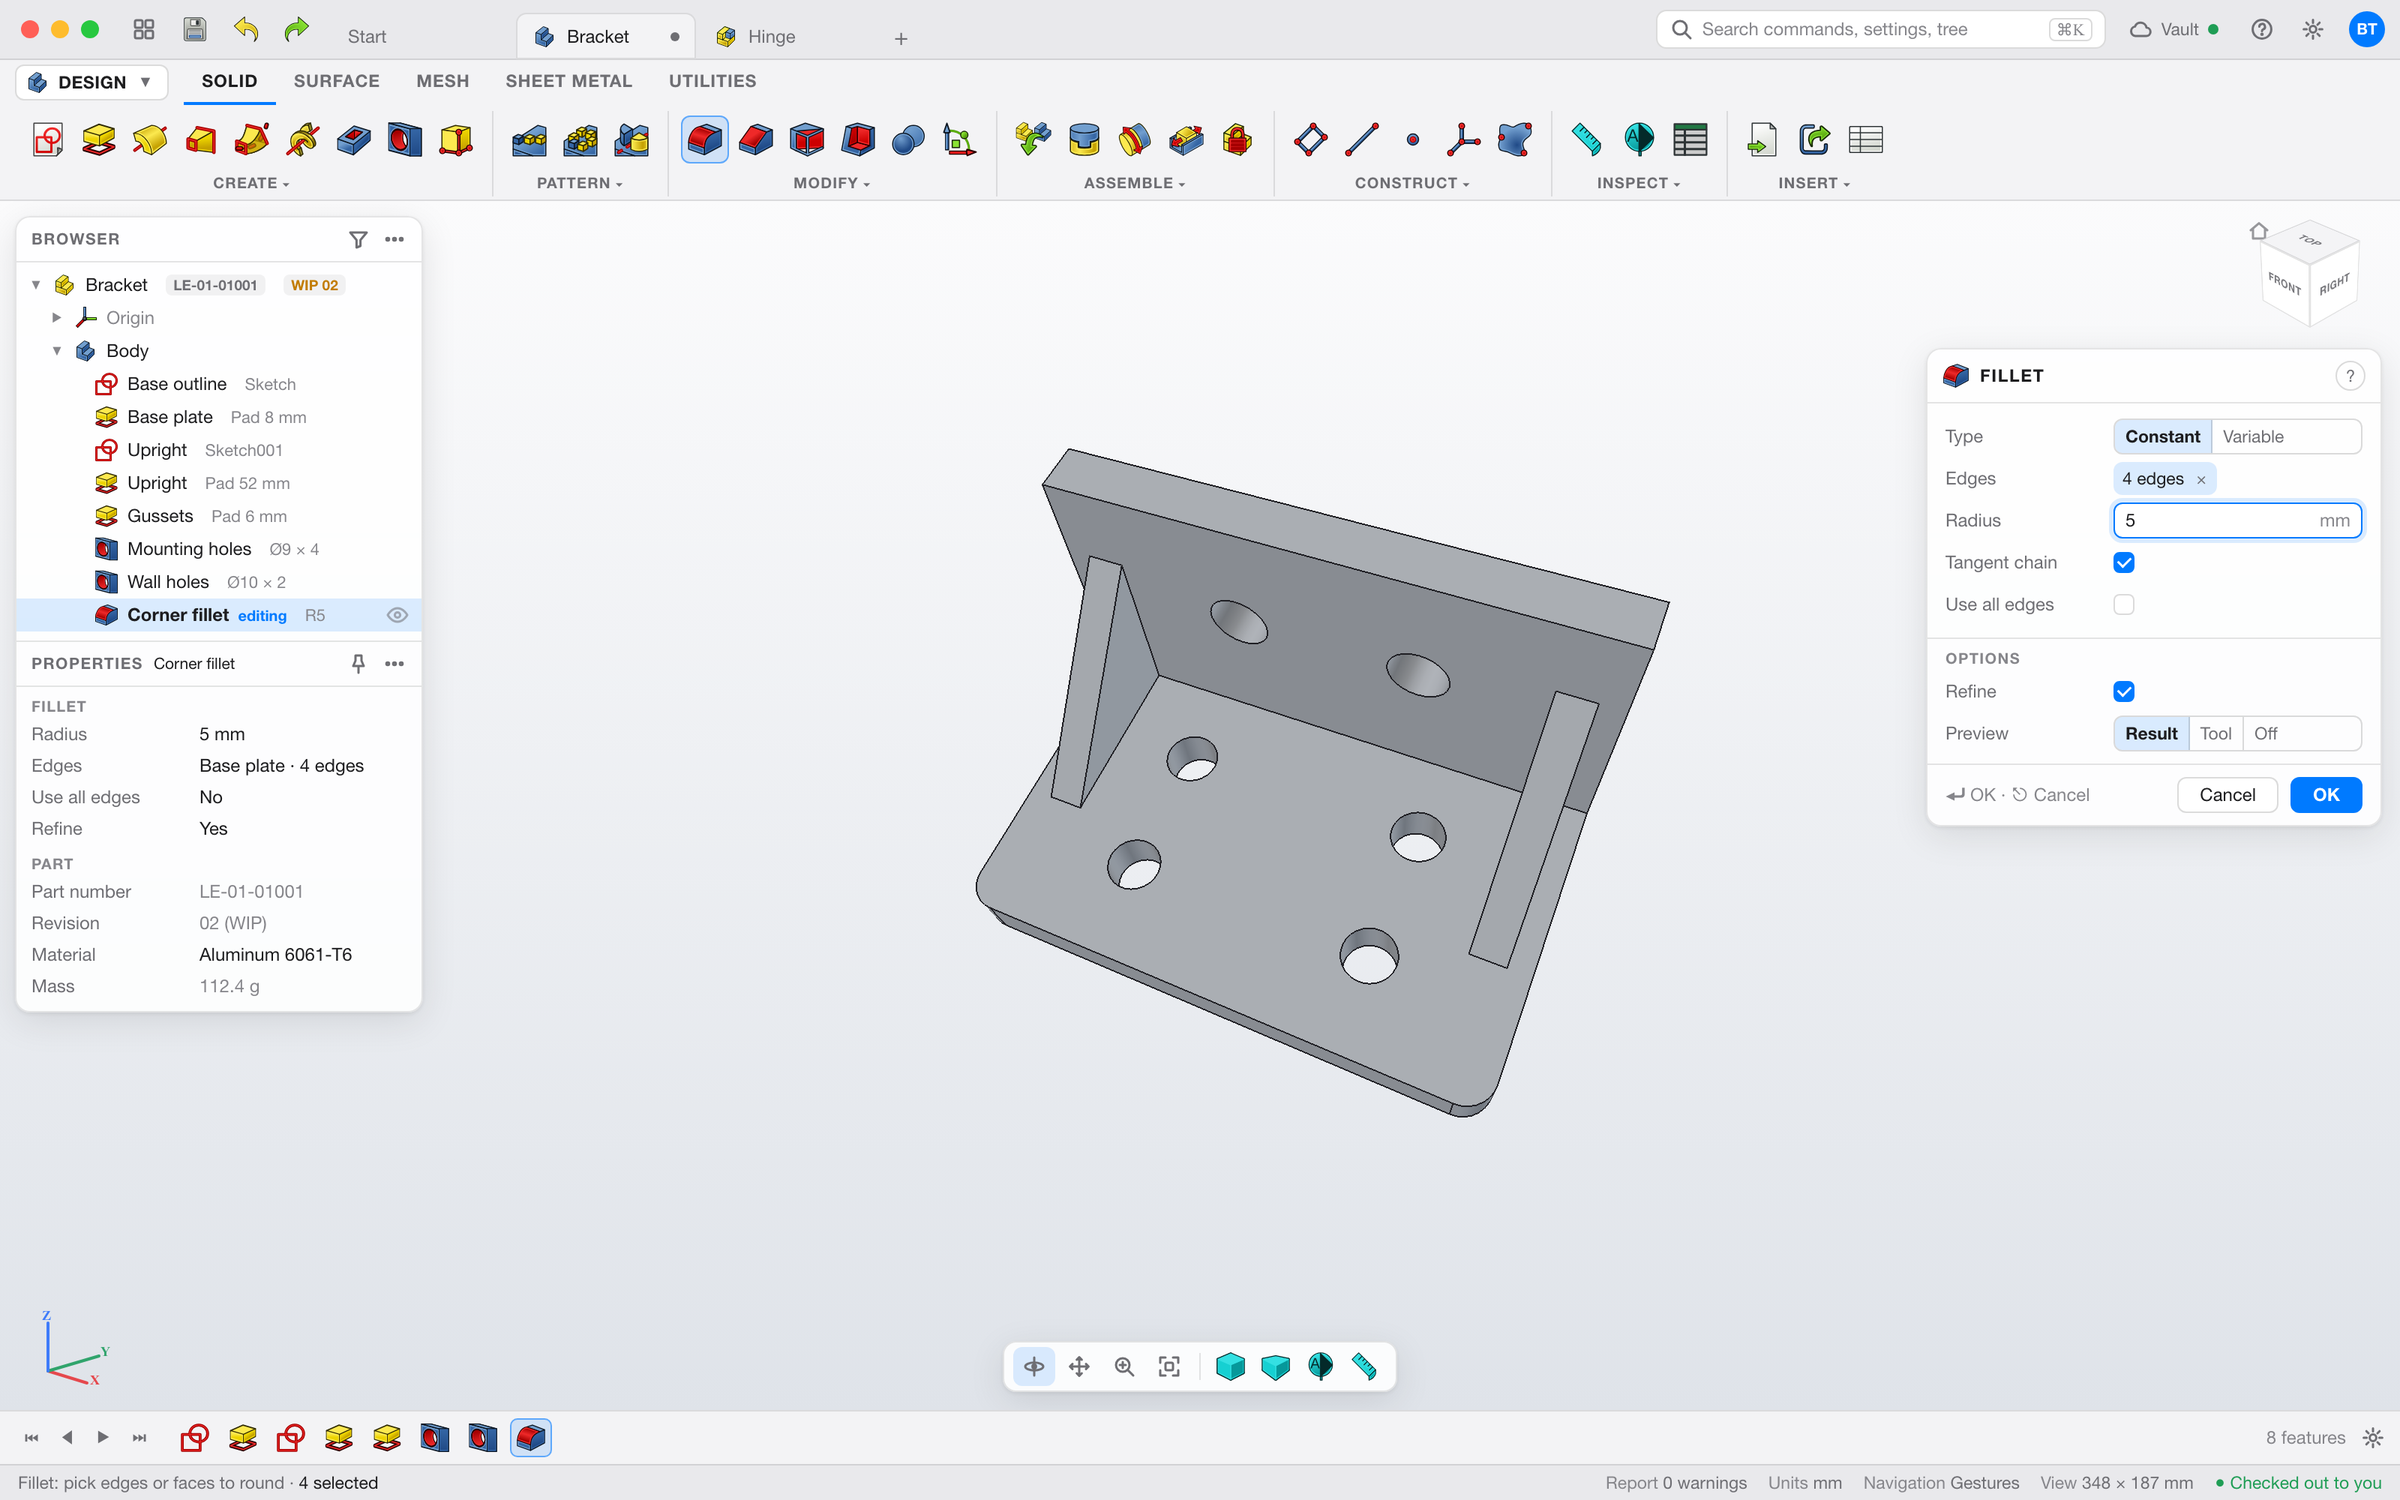
\includegraphics[width=0.497\linewidth]{fig/ui_mock_part-light.png}\hfill
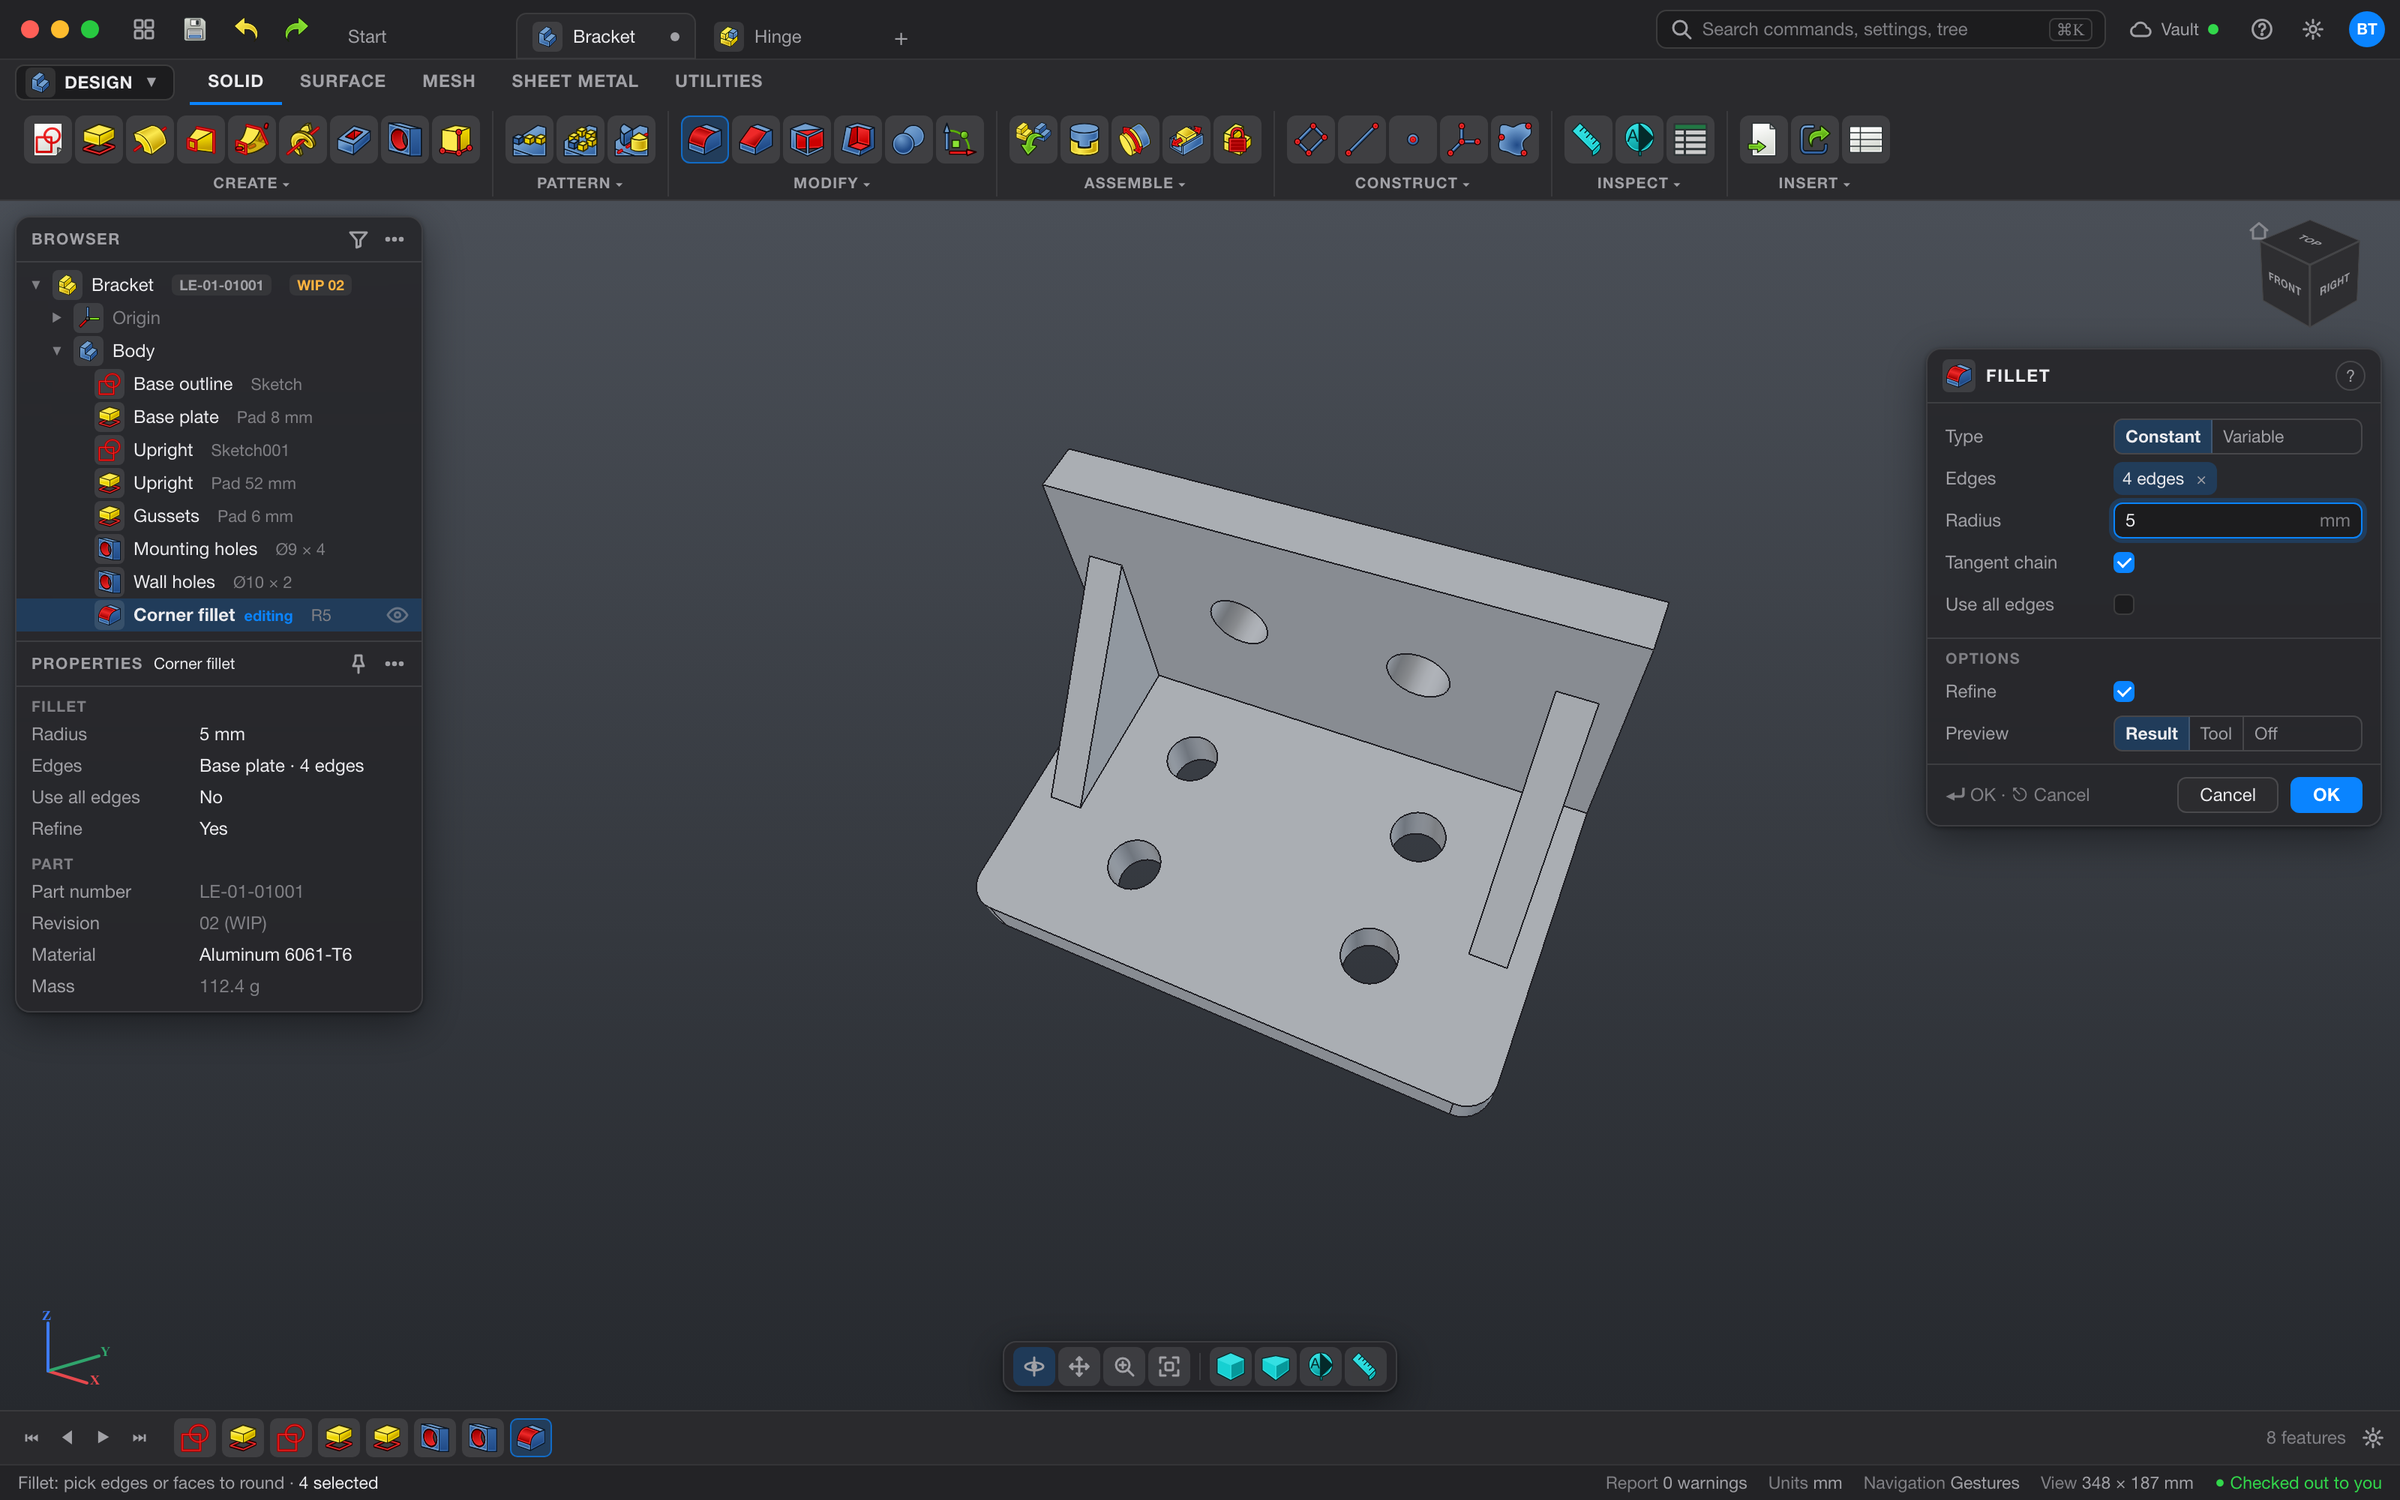
\includegraphics[width=0.497\linewidth]{fig/ui_mock_part-dark.png}\\[3pt]
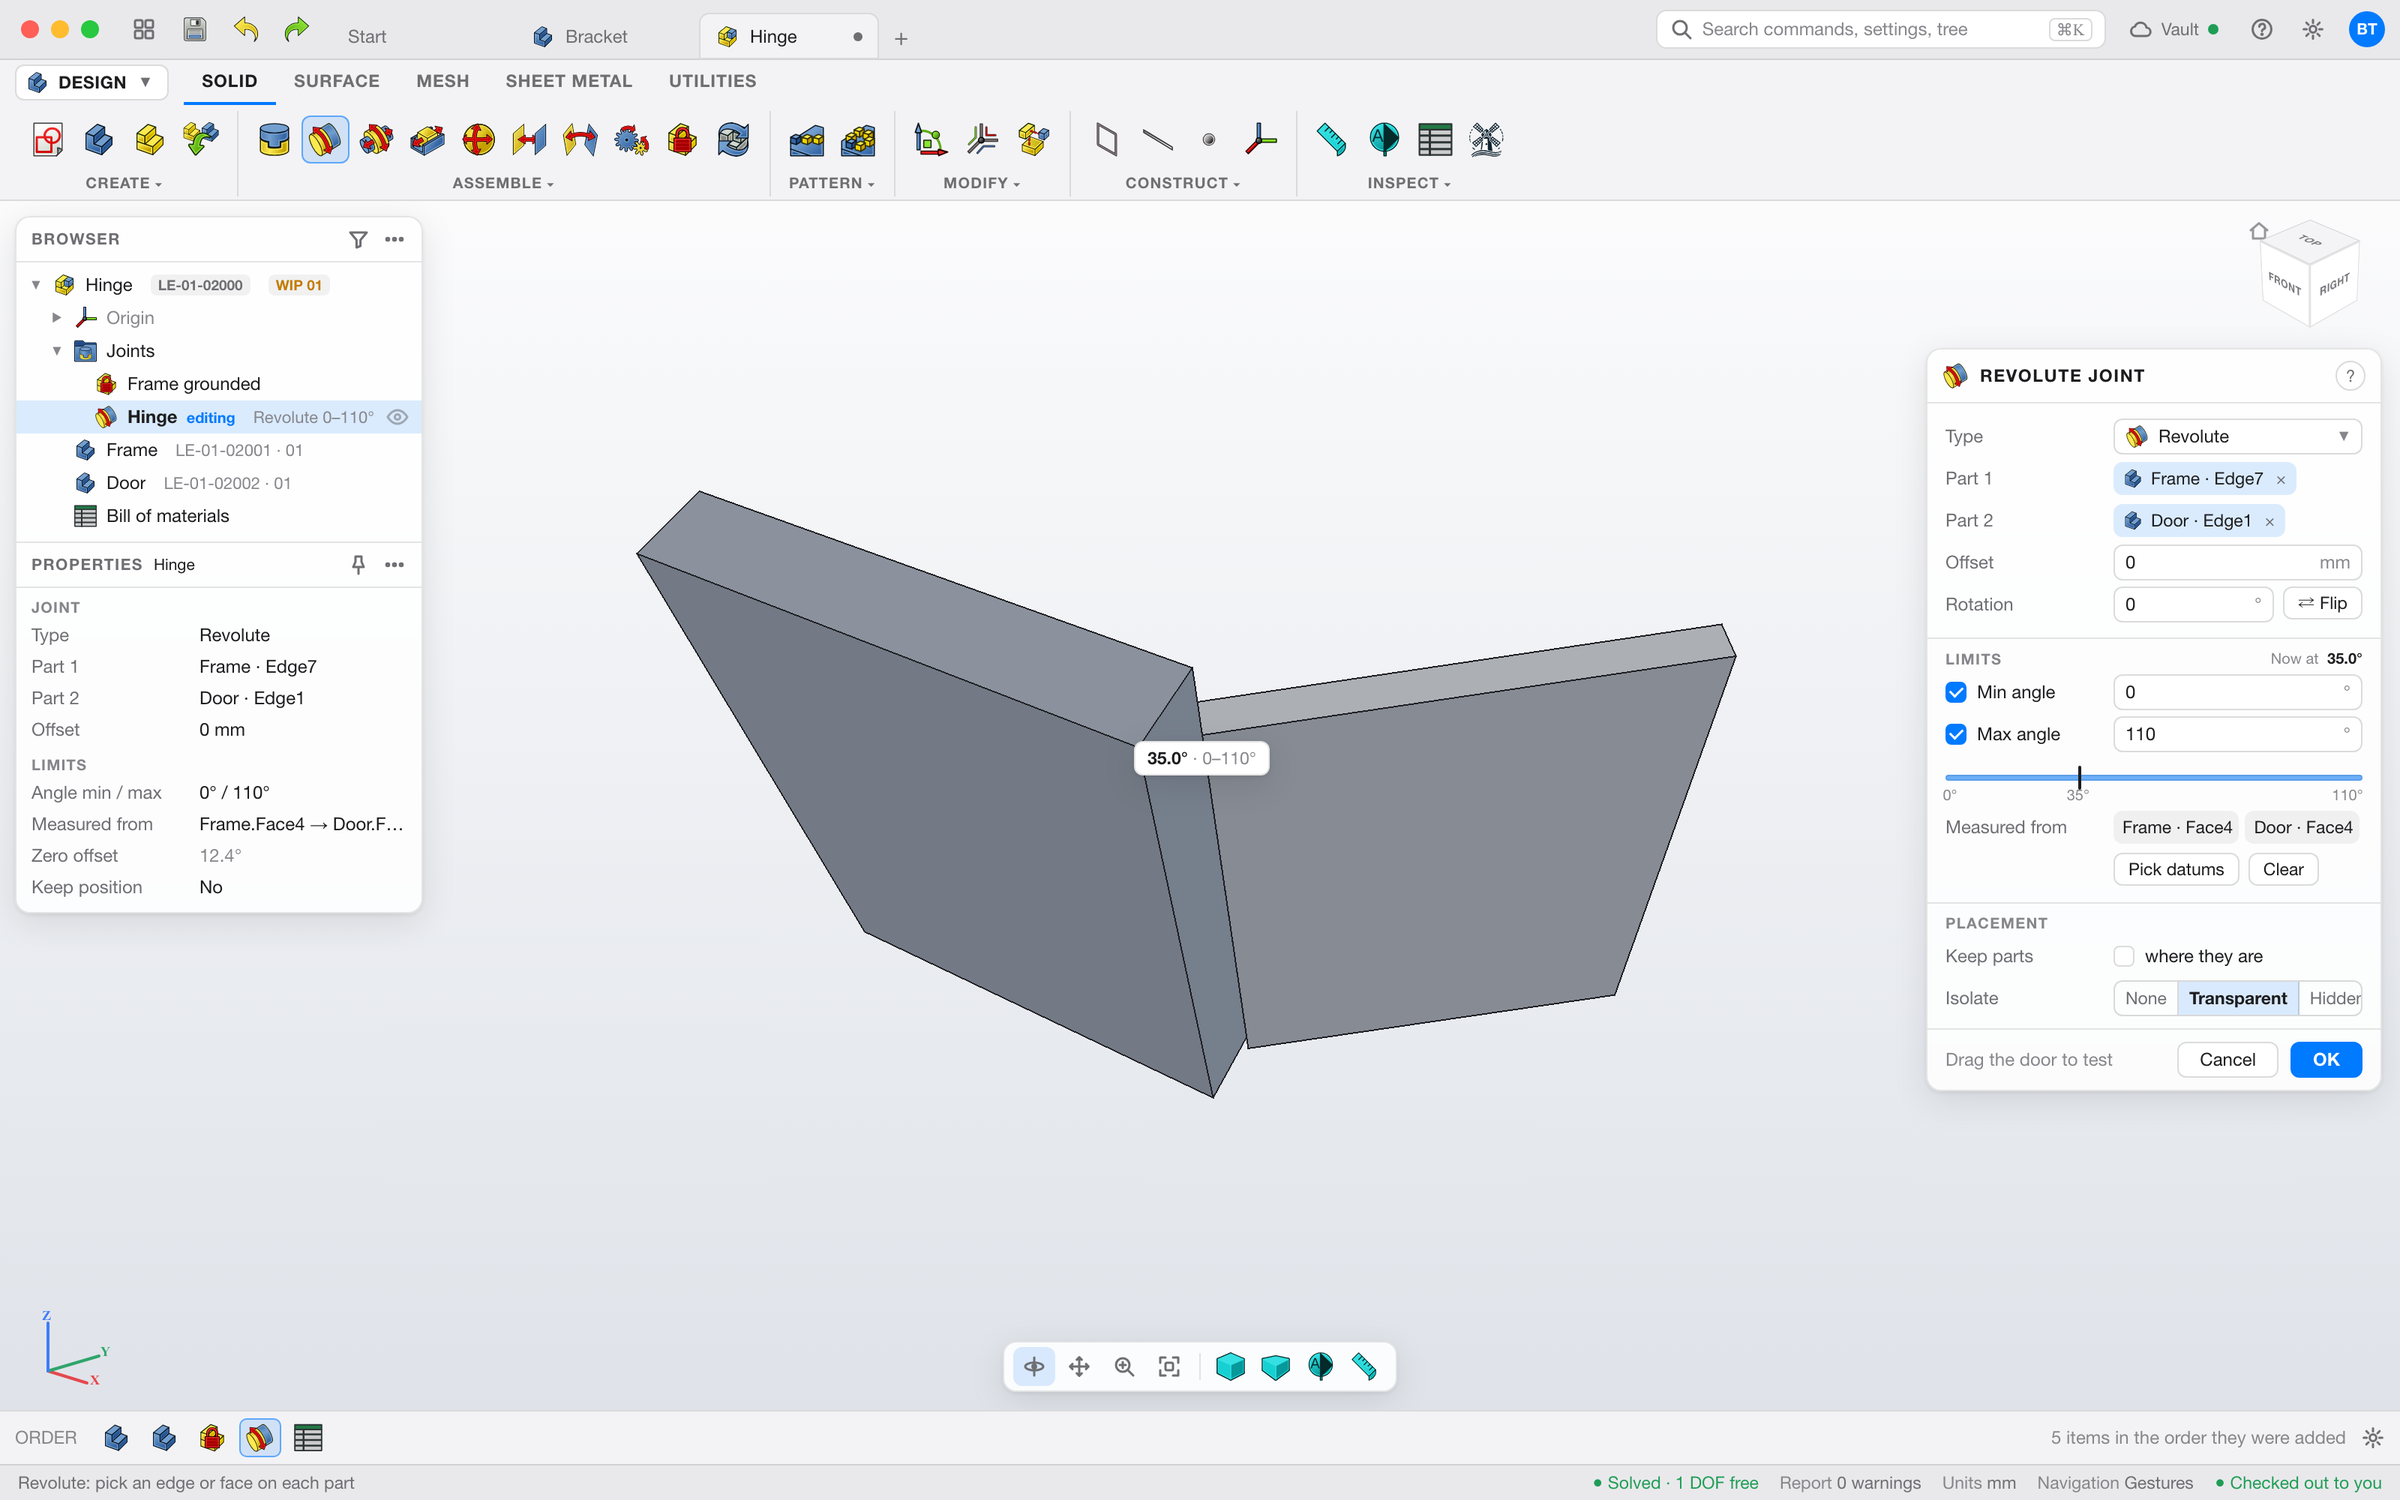
\includegraphics[width=0.497\linewidth]{fig/ui_mock_asm-light.png}\hfill
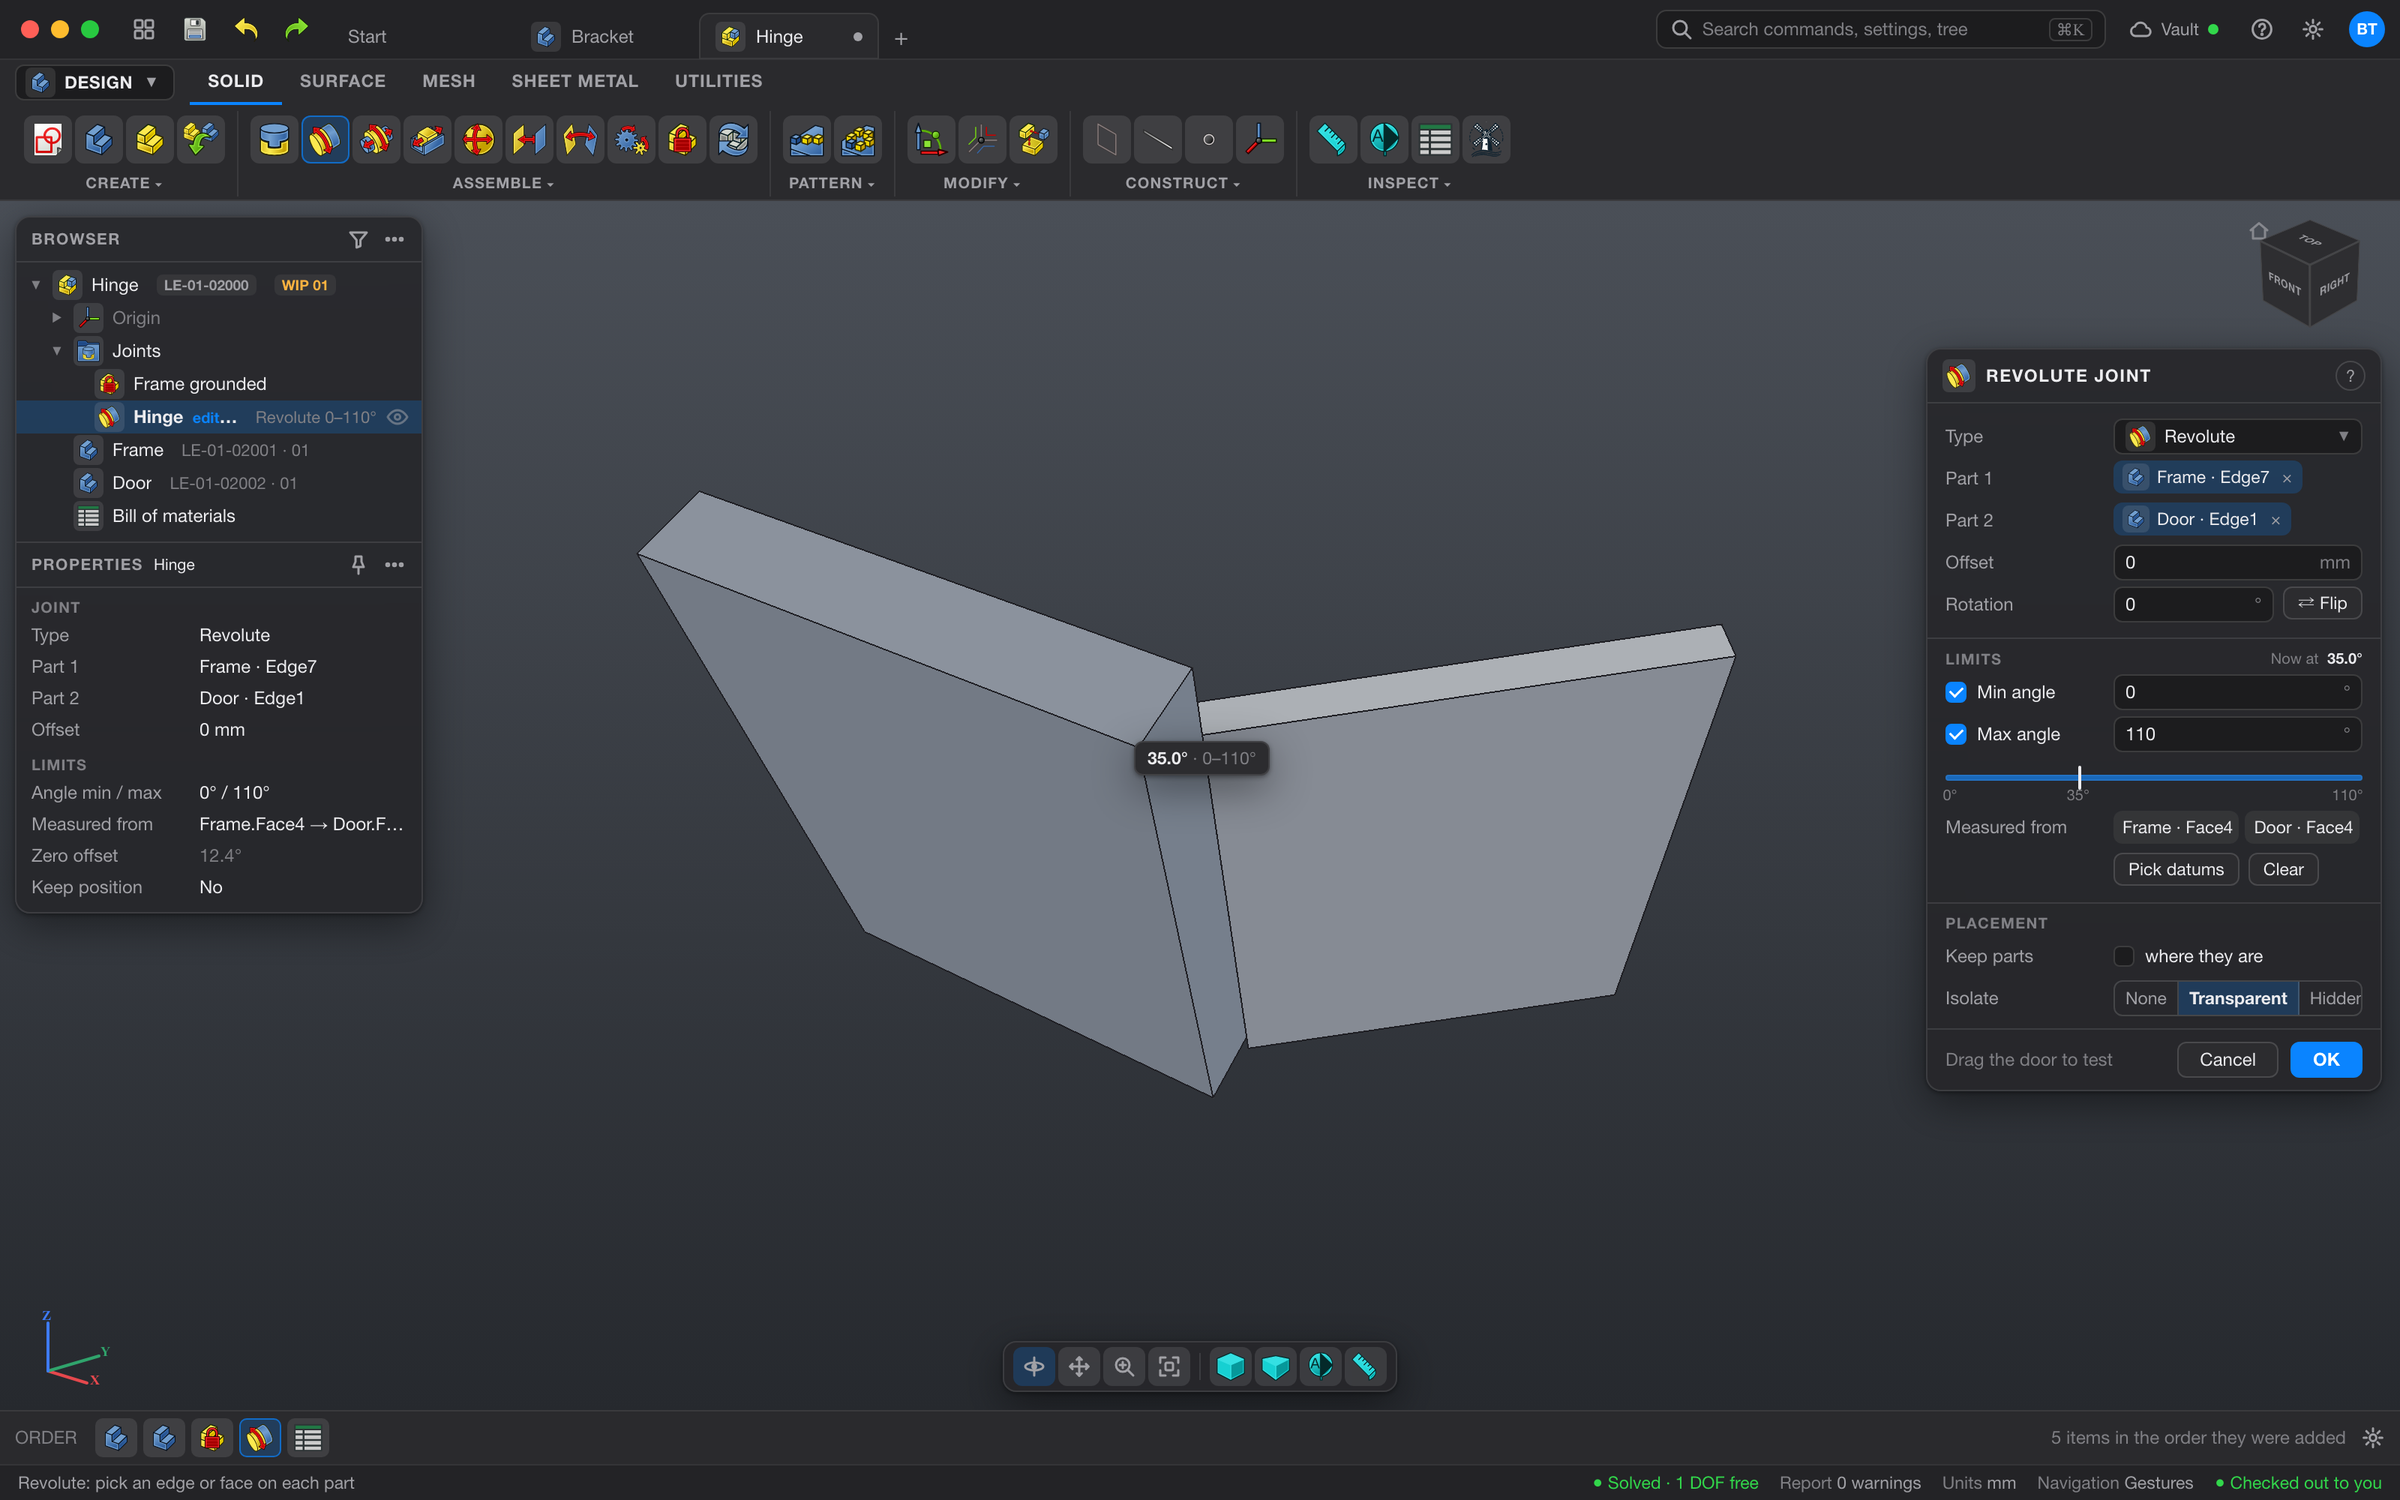
\includegraphics[width=0.497\linewidth]{fig/ui_mock_asm-dark.png}
\caption{Part modelling and assembly, light and dark. The assembly shows the Revolute joint from section
\ref{sec:joints}. The limits get a range bar with the current reading, ``Measured from'' shows both datums, and
the angle is labelled in the 3D view. Assemblies have no feature history, so the timeline row says so instead of
showing a PartDesign message.}
\label{fig:ui-part-asm}
\end{figure}

\begin{figure}[!htbp]
\centering
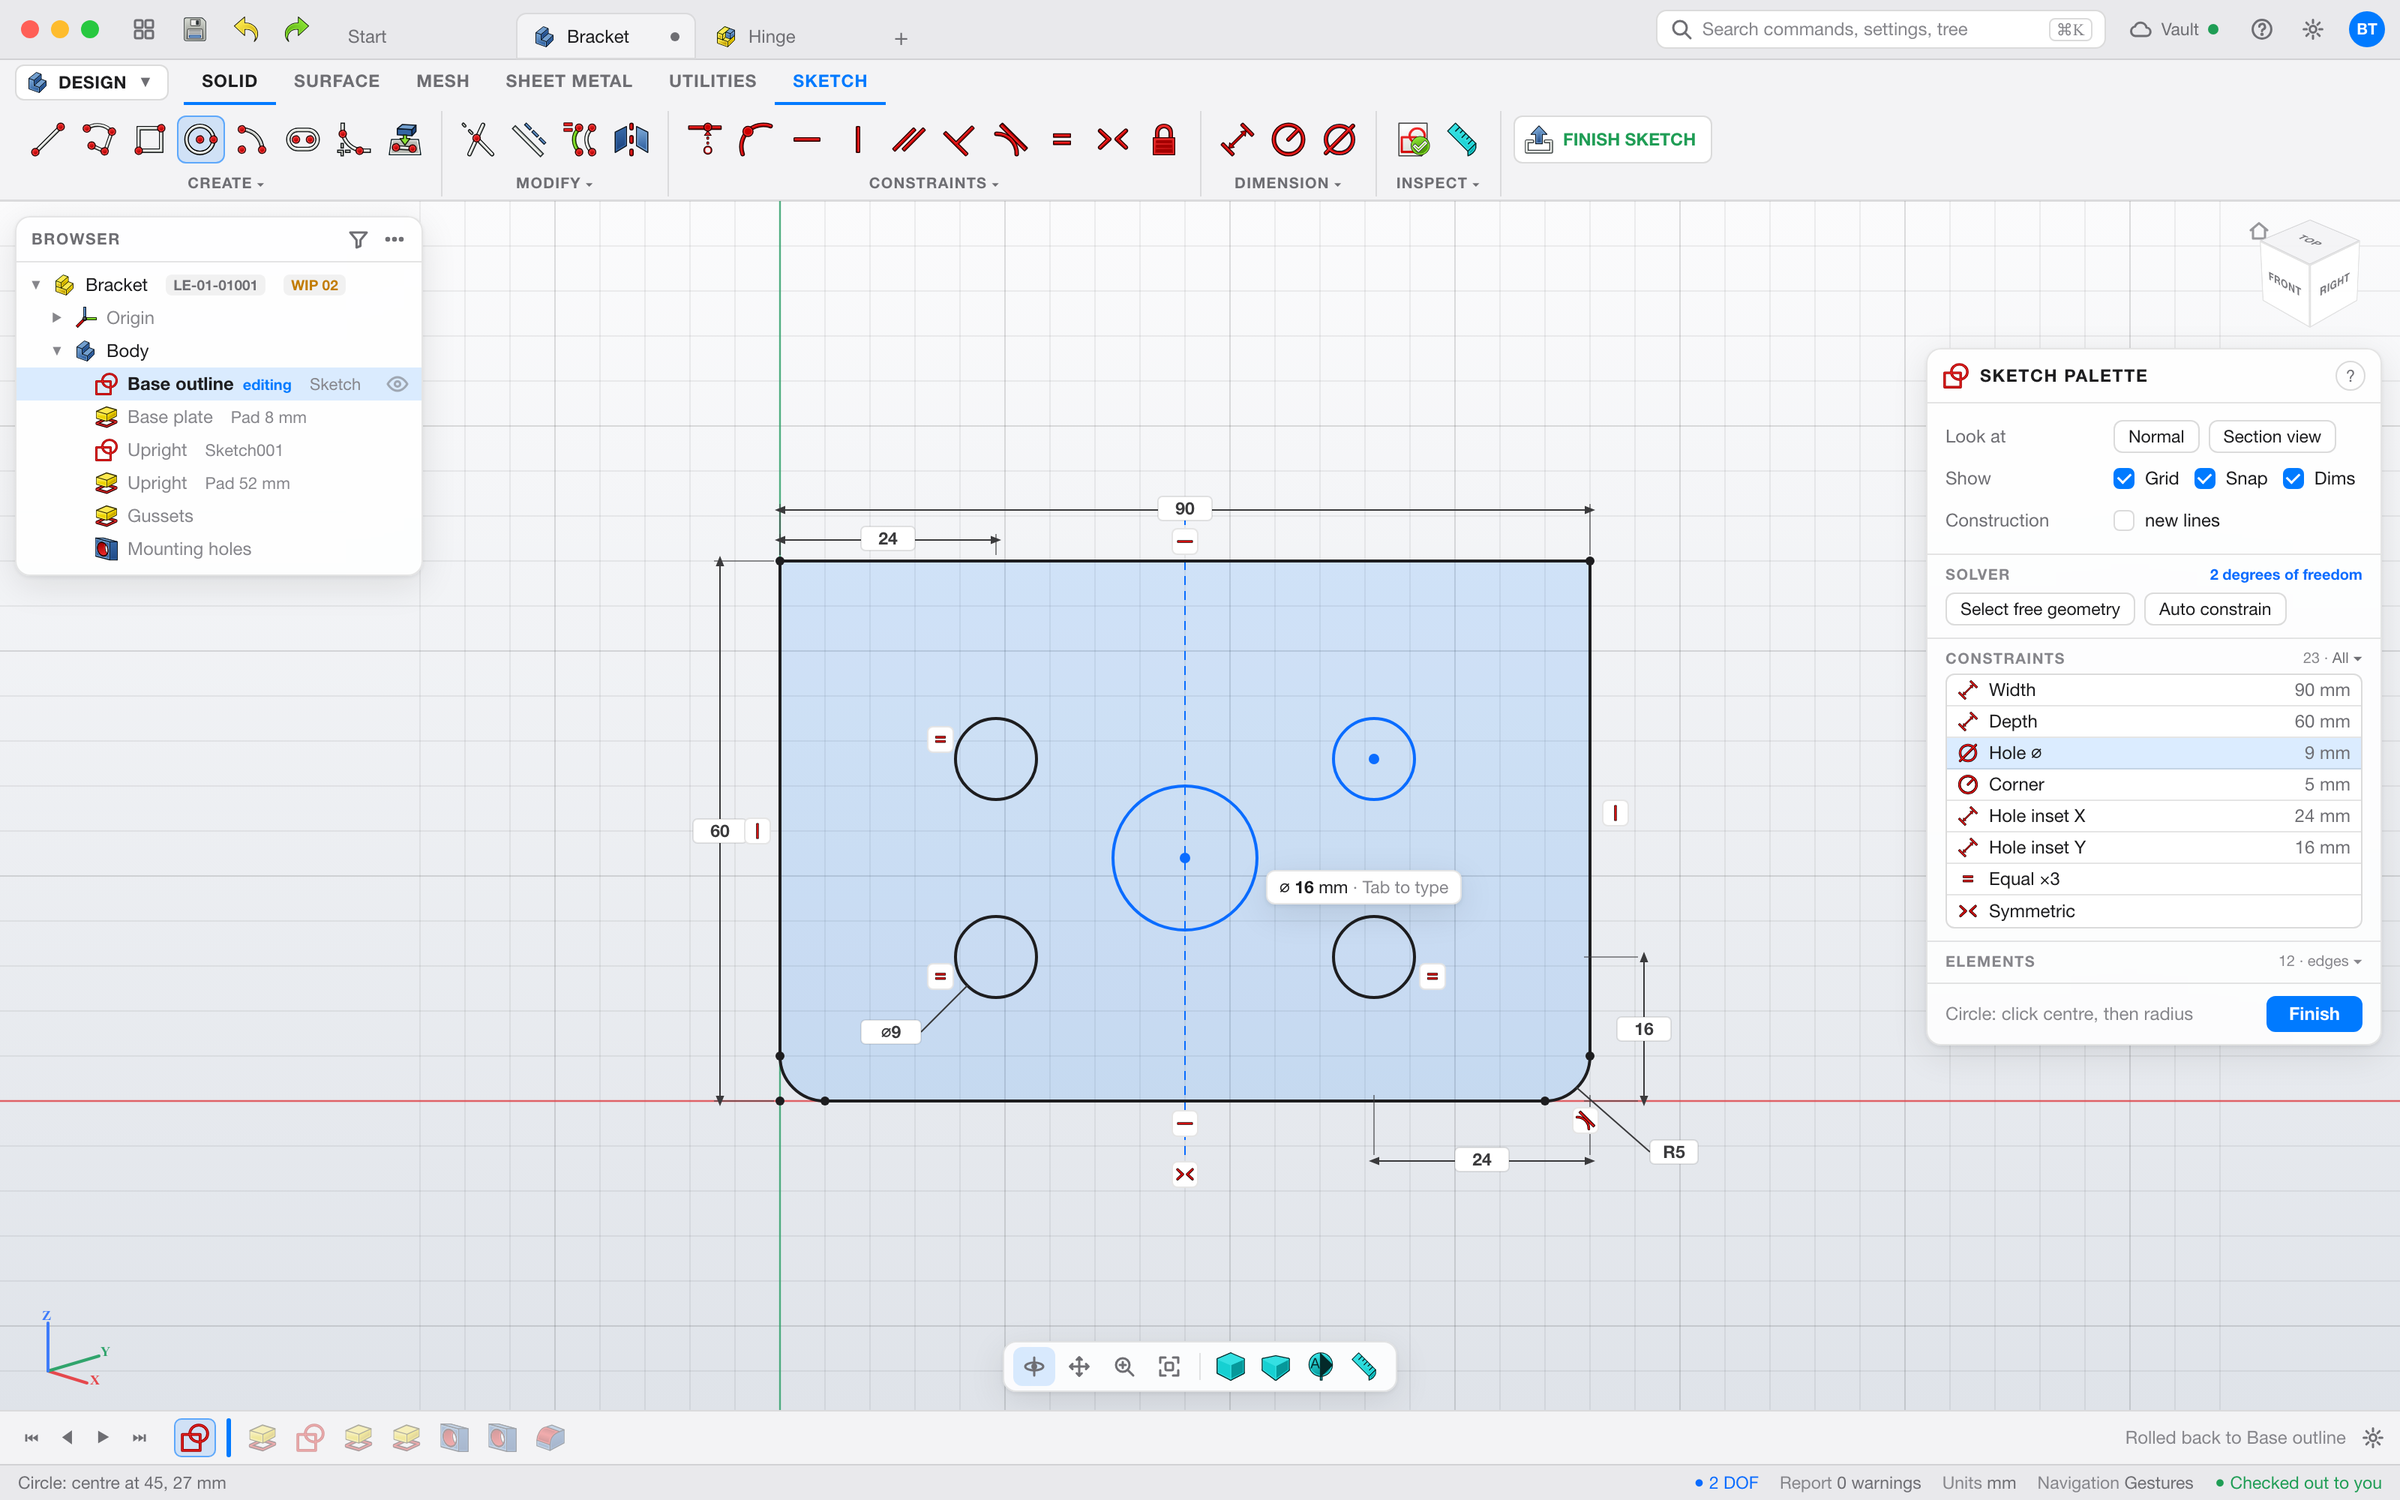
\includegraphics[width=0.497\linewidth]{fig/ui_mock_sketch-light.png}\hfill
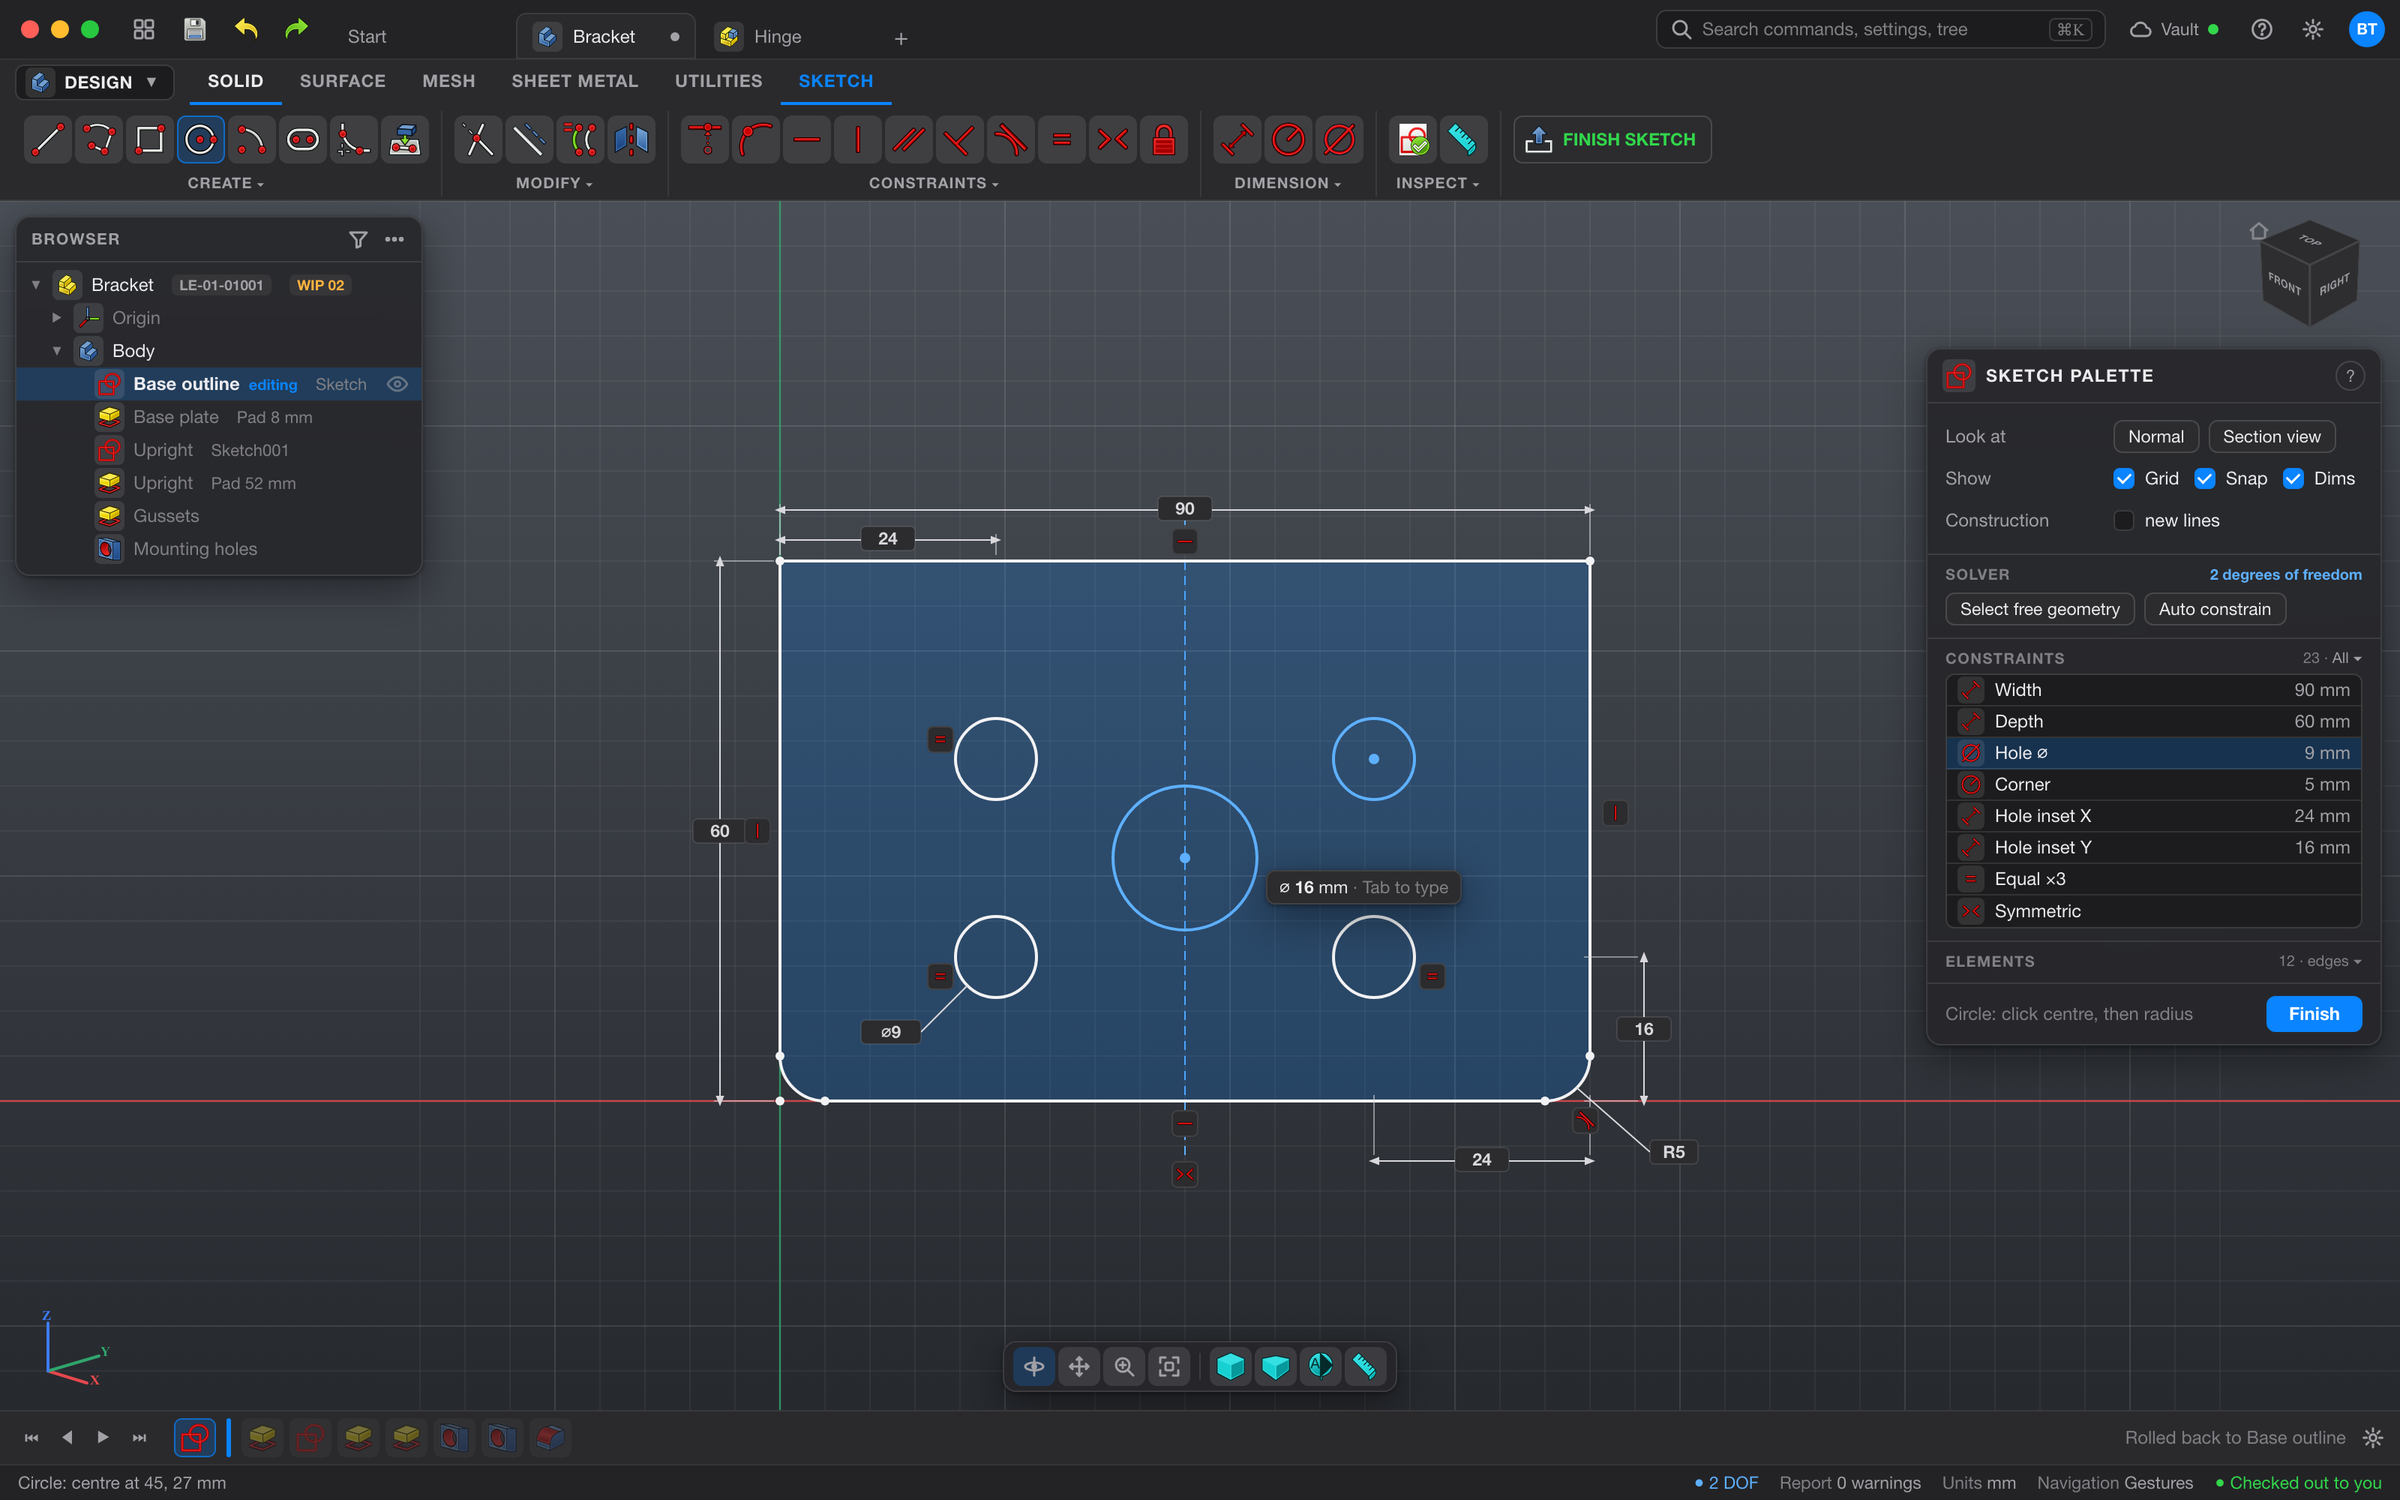
\includegraphics[width=0.497\linewidth]{fig/ui_mock_sketch-dark.png}\\[3pt]
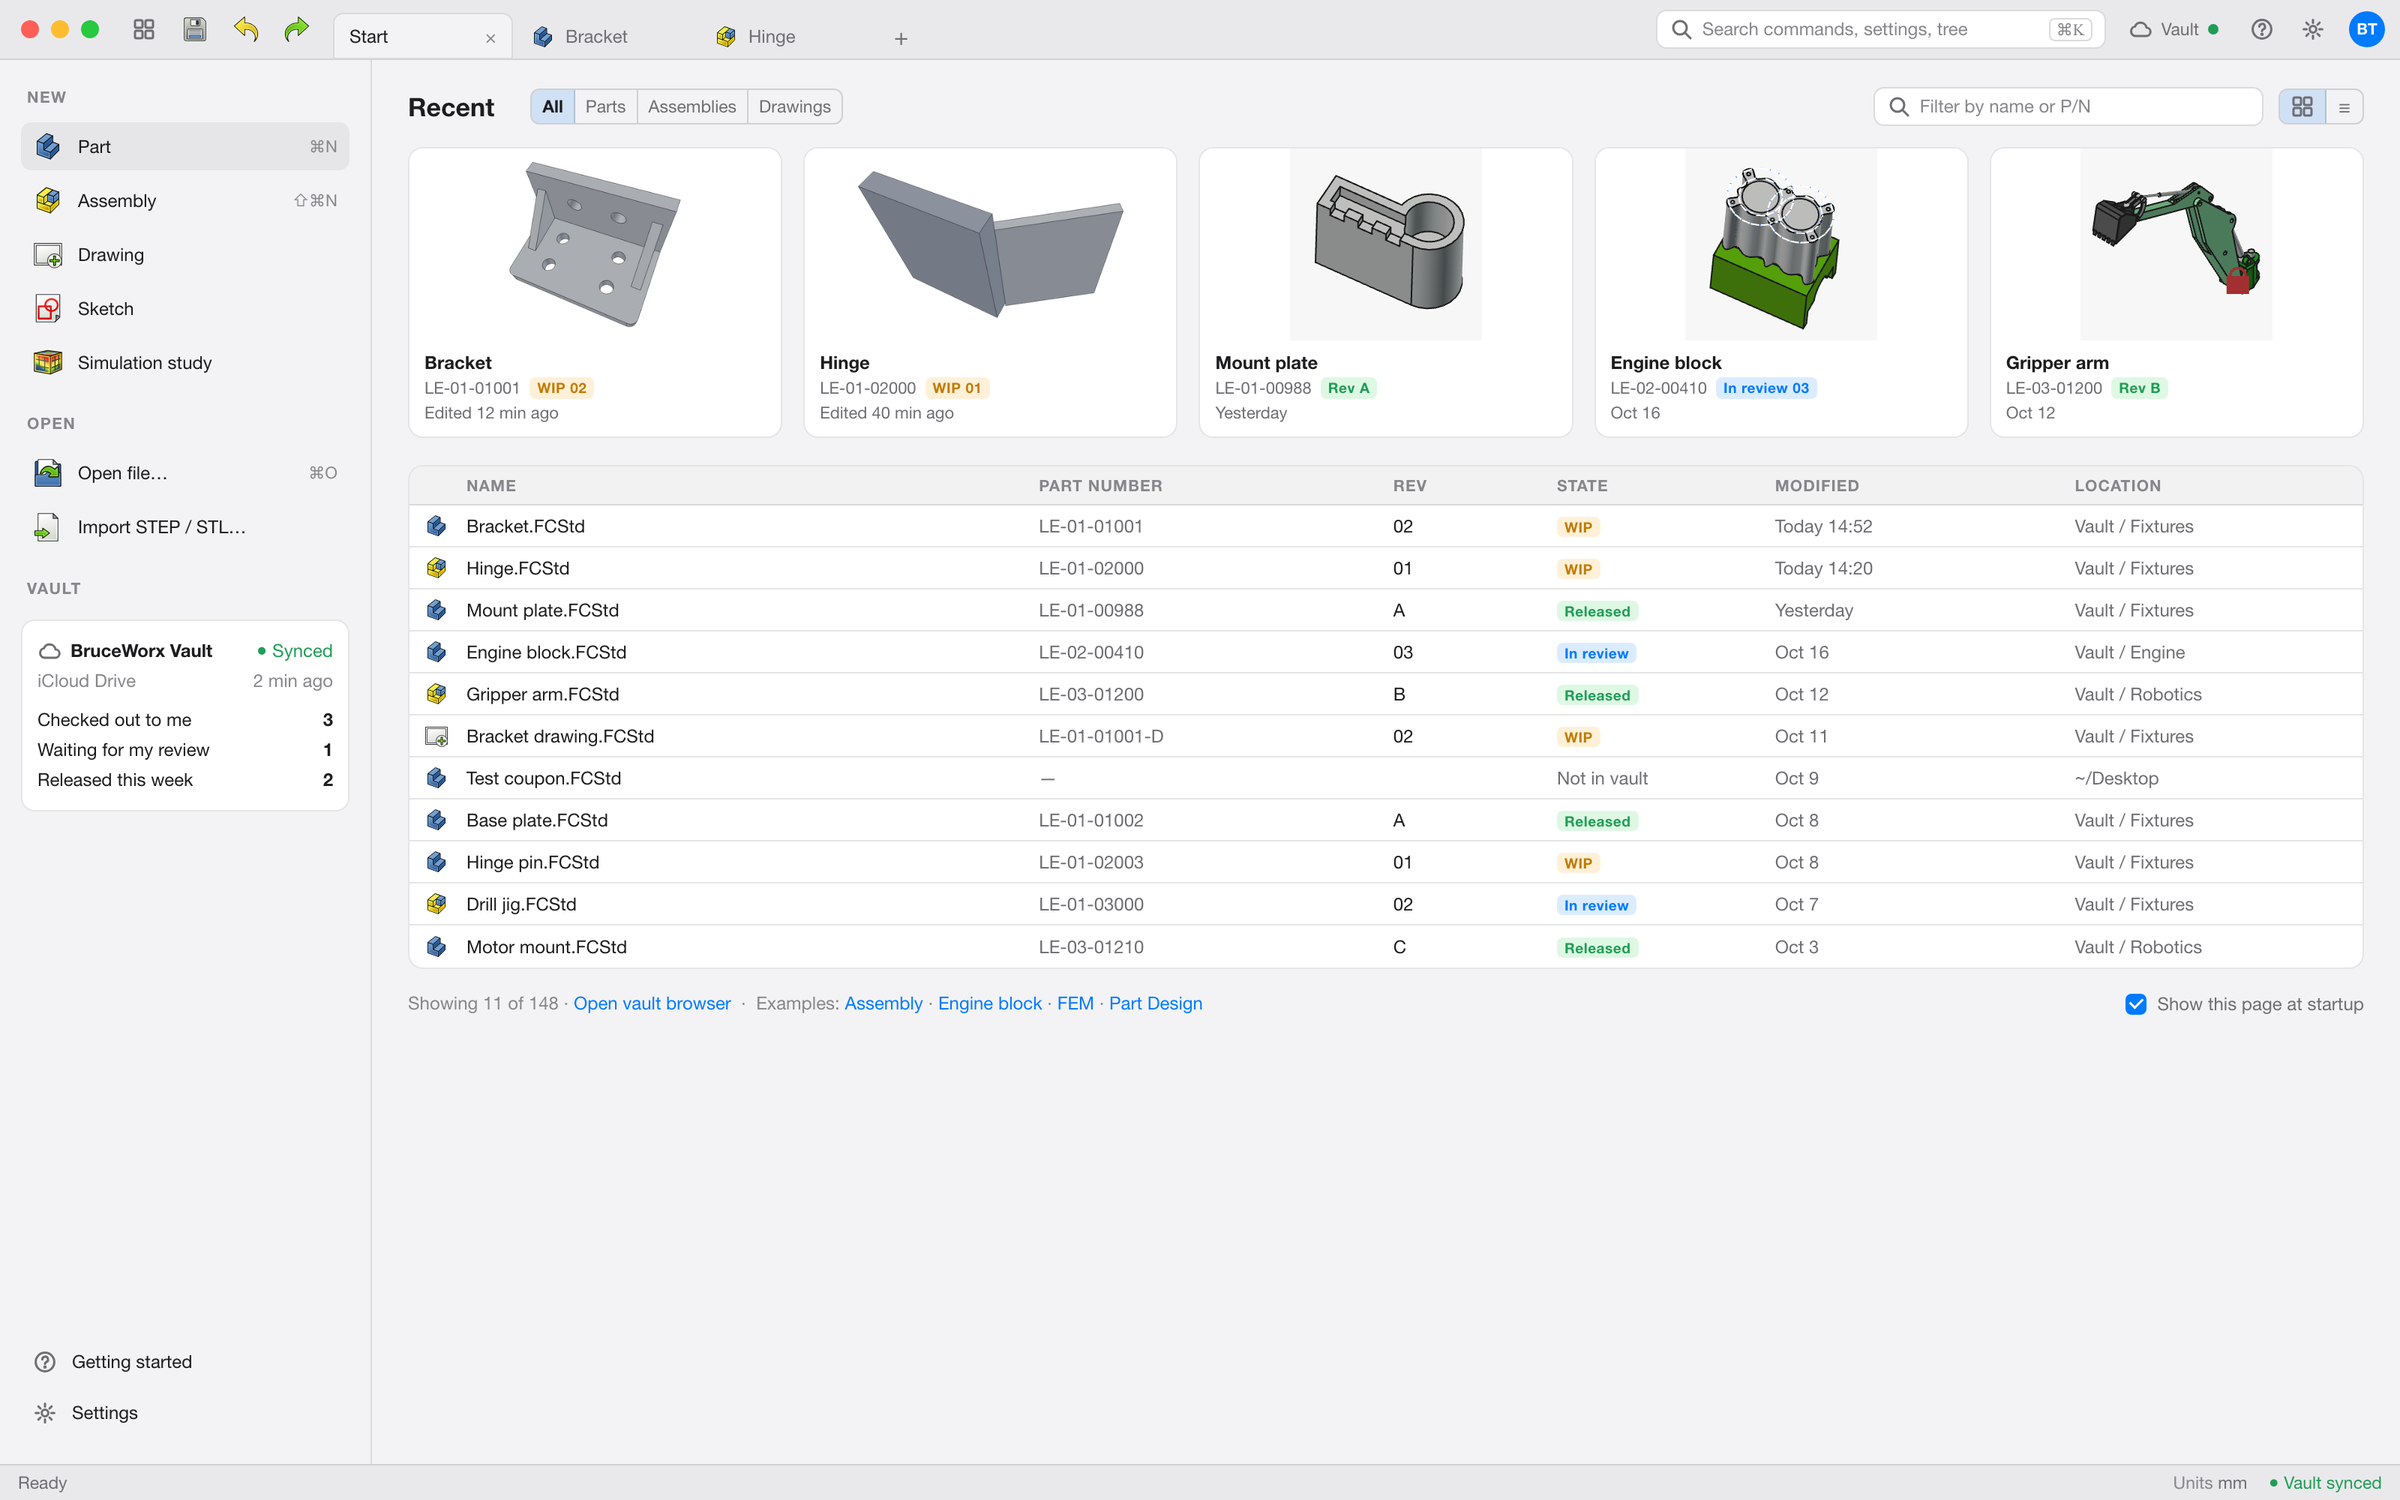
\includegraphics[width=0.497\linewidth]{fig/ui_mock_start-light.png}\hfill
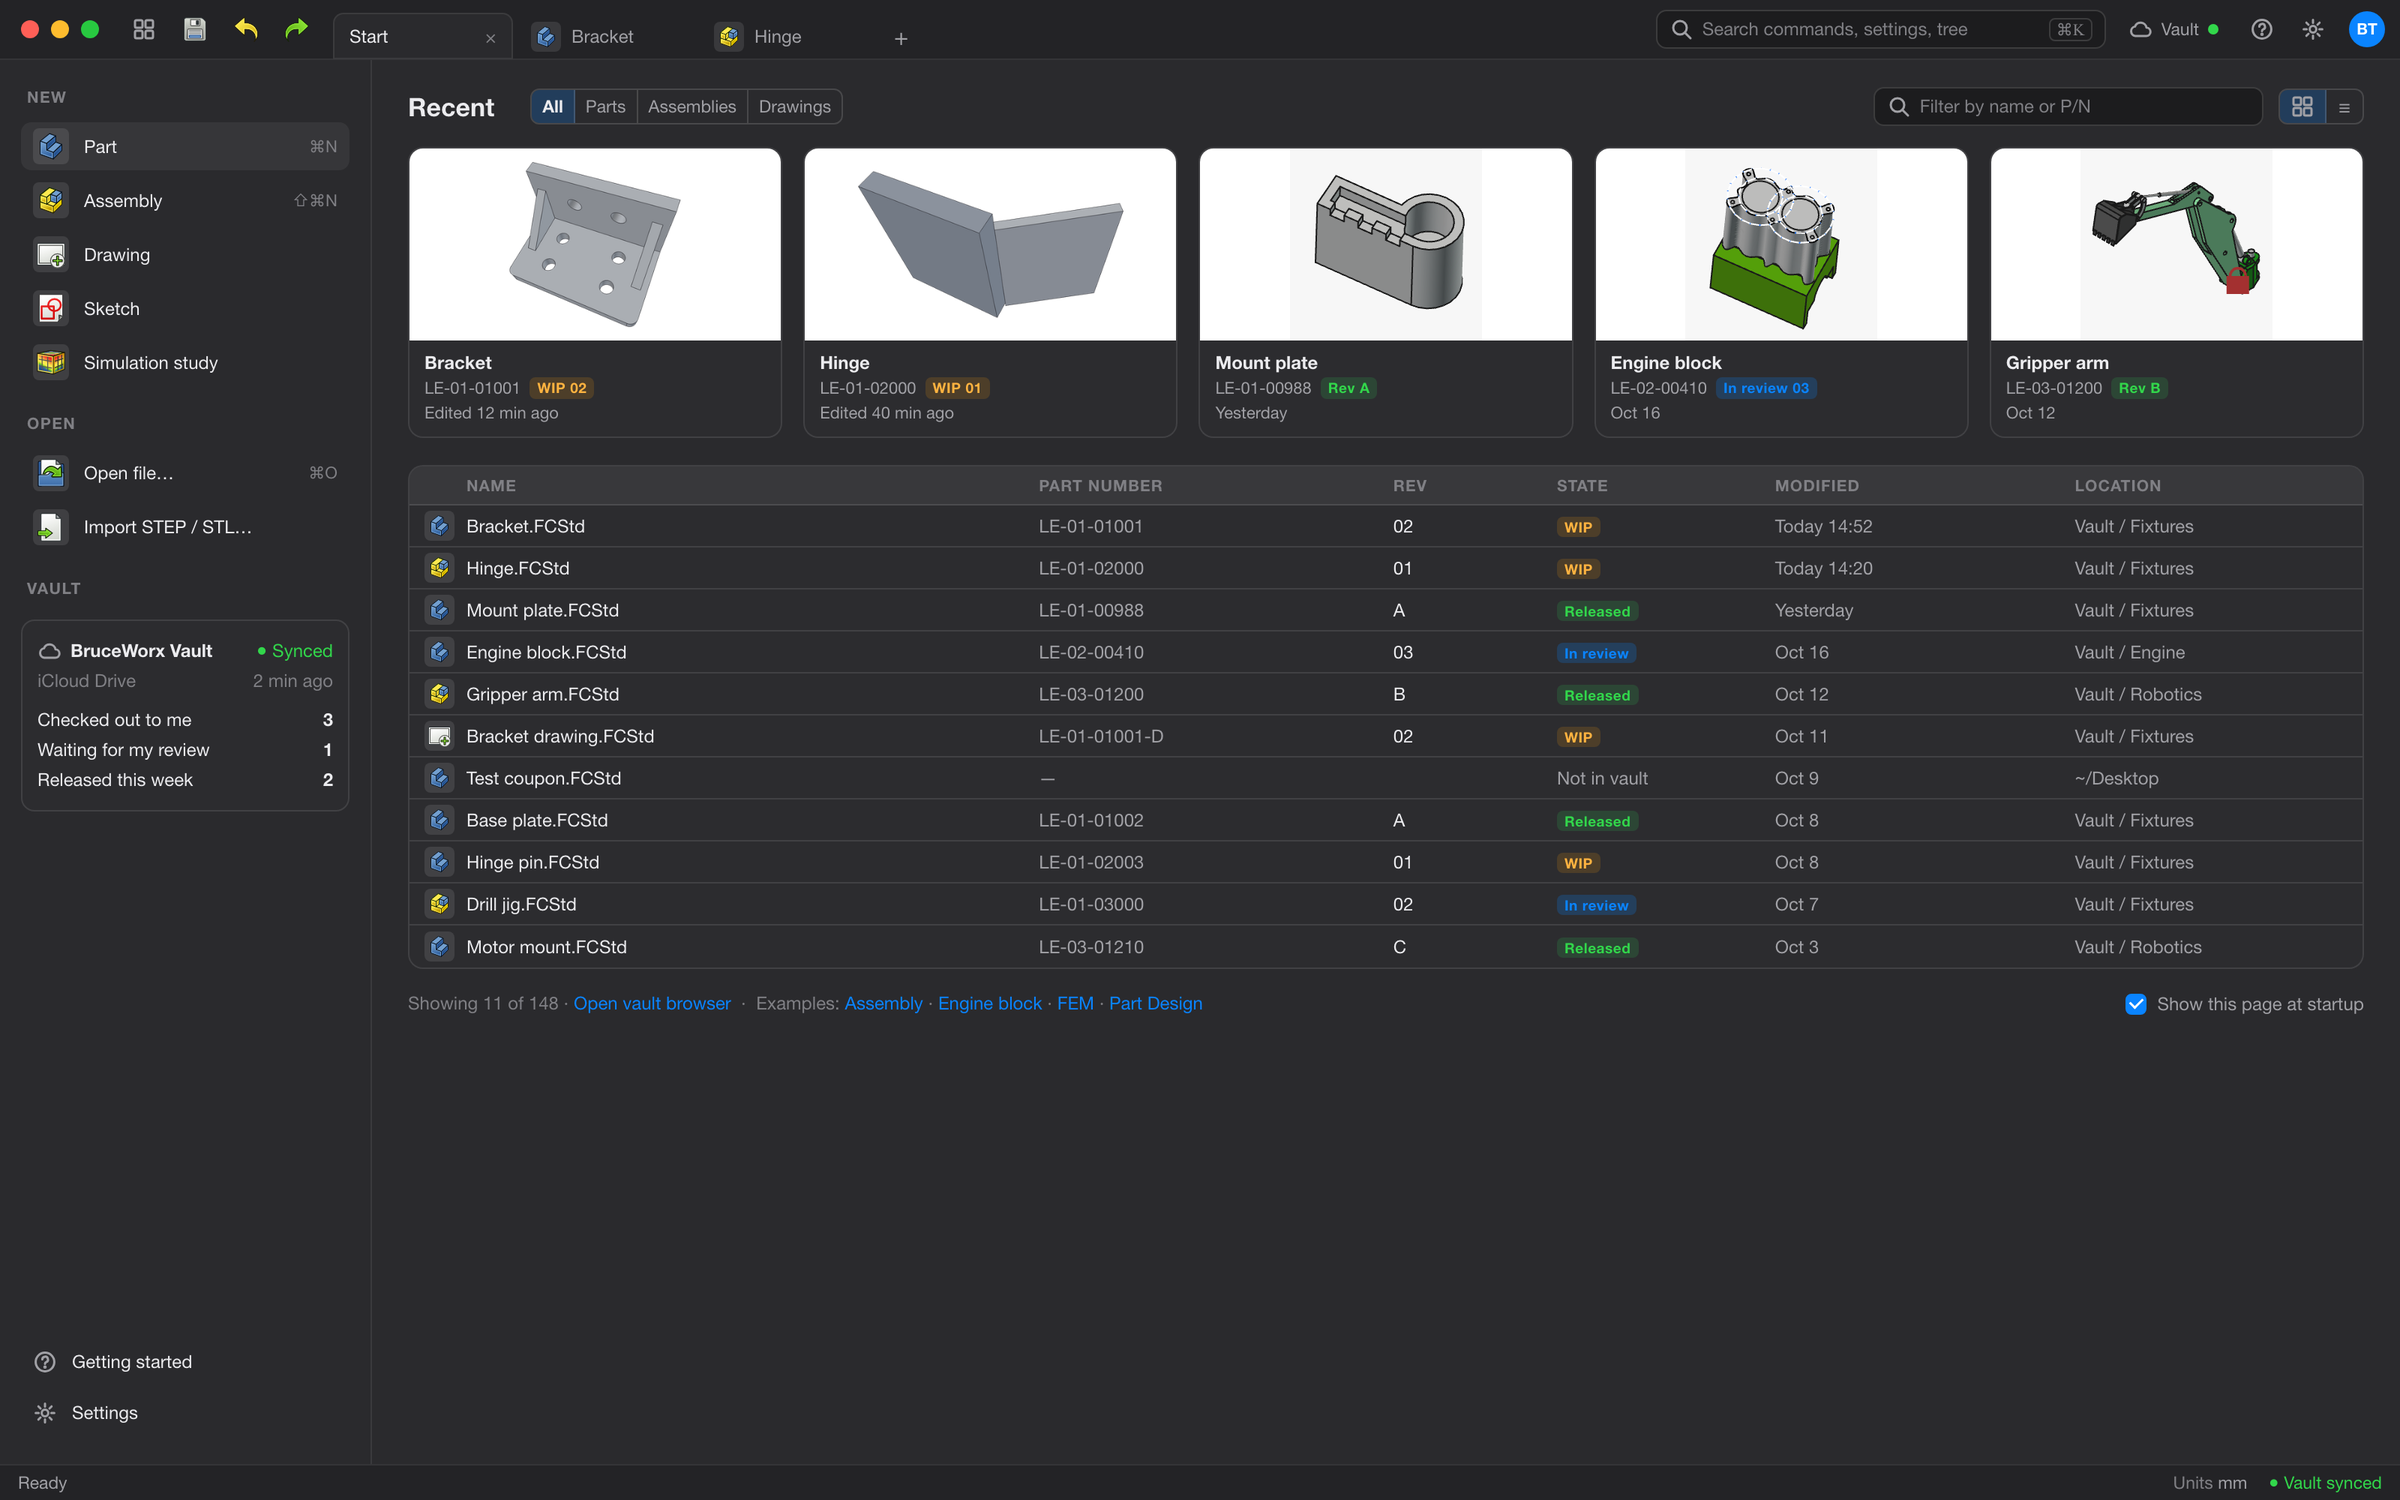
\includegraphics[width=0.497\linewidth]{fig/ui_mock_start-dark.png}
\caption{Sketch and Start page, light and dark.
\emph{Sketch:} the contextual \textsc{Sketch} tab replaces the solid tools, with \textsc{Finish Sketch} at the end. The sketch palette shows the solver (``2 degrees of freedom'', with the free geometry in blue) and a dense constraint list. The timeline is rolled back to the sketch.
\emph{Start:} new and open on the left, with the vault summary; recent files as cards, then as a table with P/N, revision and state.}
\label{fig:ui-sketch-start}
\end{figure}

\paragraph{How following the system works.} FreeCAD 1.1 has no setting for this. It applies one theme
(\file{BruceWorx.yaml} or \file{BruceWorx Dark.yaml}) and one stylesheet at start-up. This build's Qt is 6.8.3,
and Qt reports the system appearance as \code{QStyleHints::colorScheme()}, with a \code{colorSchemeChanged} signal
when you switch. BruceWorx listens for that signal. It loads the matching yaml colour tokens, re-applies
\file{BruceWorx.qss} (already written once for both themes), and sets the two viewport background colours and the
NaviCube colours. No restart is needed. The accent comes from \code{QPalette::Accent} (Qt~6.6 and later), which
on macOS is the System Settings accent. It is written into the \code{@AccentColor} token, and the derived tokens
are computed from it:
\[
  \text{accent-soft} = \alpha\,A + (1-\alpha)\,B, \qquad \alpha = 0.14 \text{ (light)},\ 0.22 \text{ (dark)},
\]
where $A$ is the accent and $B$ the card colour. Selected rows, pressed tools and chips use accent-soft. Only the
default button, checkboxes and the focus ring use the full accent.

\paragraph{Contrast, checked rather than eyeballed.} With a user-chosen accent, text on it can become
unreadable (white on yellow). The rule uses the WCAG relative luminance of each colour,
\[
  L = 0.2126\,R + 0.7152\,G + 0.0722\,B, \qquad c = \begin{cases} c_s/12.92 & c_s \le 0.04045\\ \left(\tfrac{c_s+0.055}{1.055}\right)^{2.4} & \text{otherwise}\end{cases}
\]
for each sRGB channel $c_s \in [0,1]$, and the contrast ratio $C = (L_1+0.05)/(L_2+0.05)$ with $L_1 \ge L_2$.
Text on the accent is white when $C_\text{white} \ge 3$ (macOS's own choice for buttons), otherwise near-black.

\begin{center}
\small
\begin{tabular}{@{}lrr@{\qquad}lrrl@{}}
\toprule
Text on card & Light & Dark & macOS accent & White & Black & Text\\
\midrule
Primary & 16.8 & 11.8 & Blue & 4.02 & 5.23 & white\\
Secondary & 5.1 & 5.4 & Purple & 4.88 & 4.31 & white\\
Tertiary (hints) & 3.6 & 3.5 & Pink / Red & 3.20 / 3.18 & 6.6 & white\\
\textit{Faded tree today} & \textit{1.1} & --- & Orange & 2.57 & 8.16 & black\\
 & & & Yellow / Green & 1.58 / 2.43 & 13.3 / 8.6 & black\\
\bottomrule
\end{tabular}
\end{center}
The mock's tertiary grey was darkened from 2.6:1 to 3.6:1 by this check. The accent values are Apple's published
light-mode colours. \verify

\begin{center}
\small
\begin{tabular}{@{}lll@{\qquad}lll@{}}
\toprule
Token & Light & Dark & Token & Light & Dark\\
\midrule
Chrome & \code{\#E9E9EC} & \code{\#232326} & Text & \code{\#1D1D1F} & \code{\#ECECEF}\\
Toolbar & \code{\#F3F3F5} & \code{\#2A2A2D} & Text 2 & \code{\#6E6E73} & \code{\#A1A1A6}\\
Card & white 88\,\% & \code{\#262629} 90\,\% & Text 3 & \code{\#86868B} & \code{\#808085}\\
Field & \code{\#FFFFFF} & \code{\#1C1C1E} & Accent & system & system\\
Viewport top & \code{\#FBFBFC} & \code{\#4A4F57} & OK & \code{\#1F9D55} & \code{\#32D74B}\\
Viewport bottom & \code{\#DFE3E9} & \code{\#26292E} & WIP & \code{\#C27C00} & \code{\#FFB340}\\
\bottomrule
\end{tabular}
\end{center}

\subsubsection*{Before and after}

\begin{figure}[!htbp]
\centering
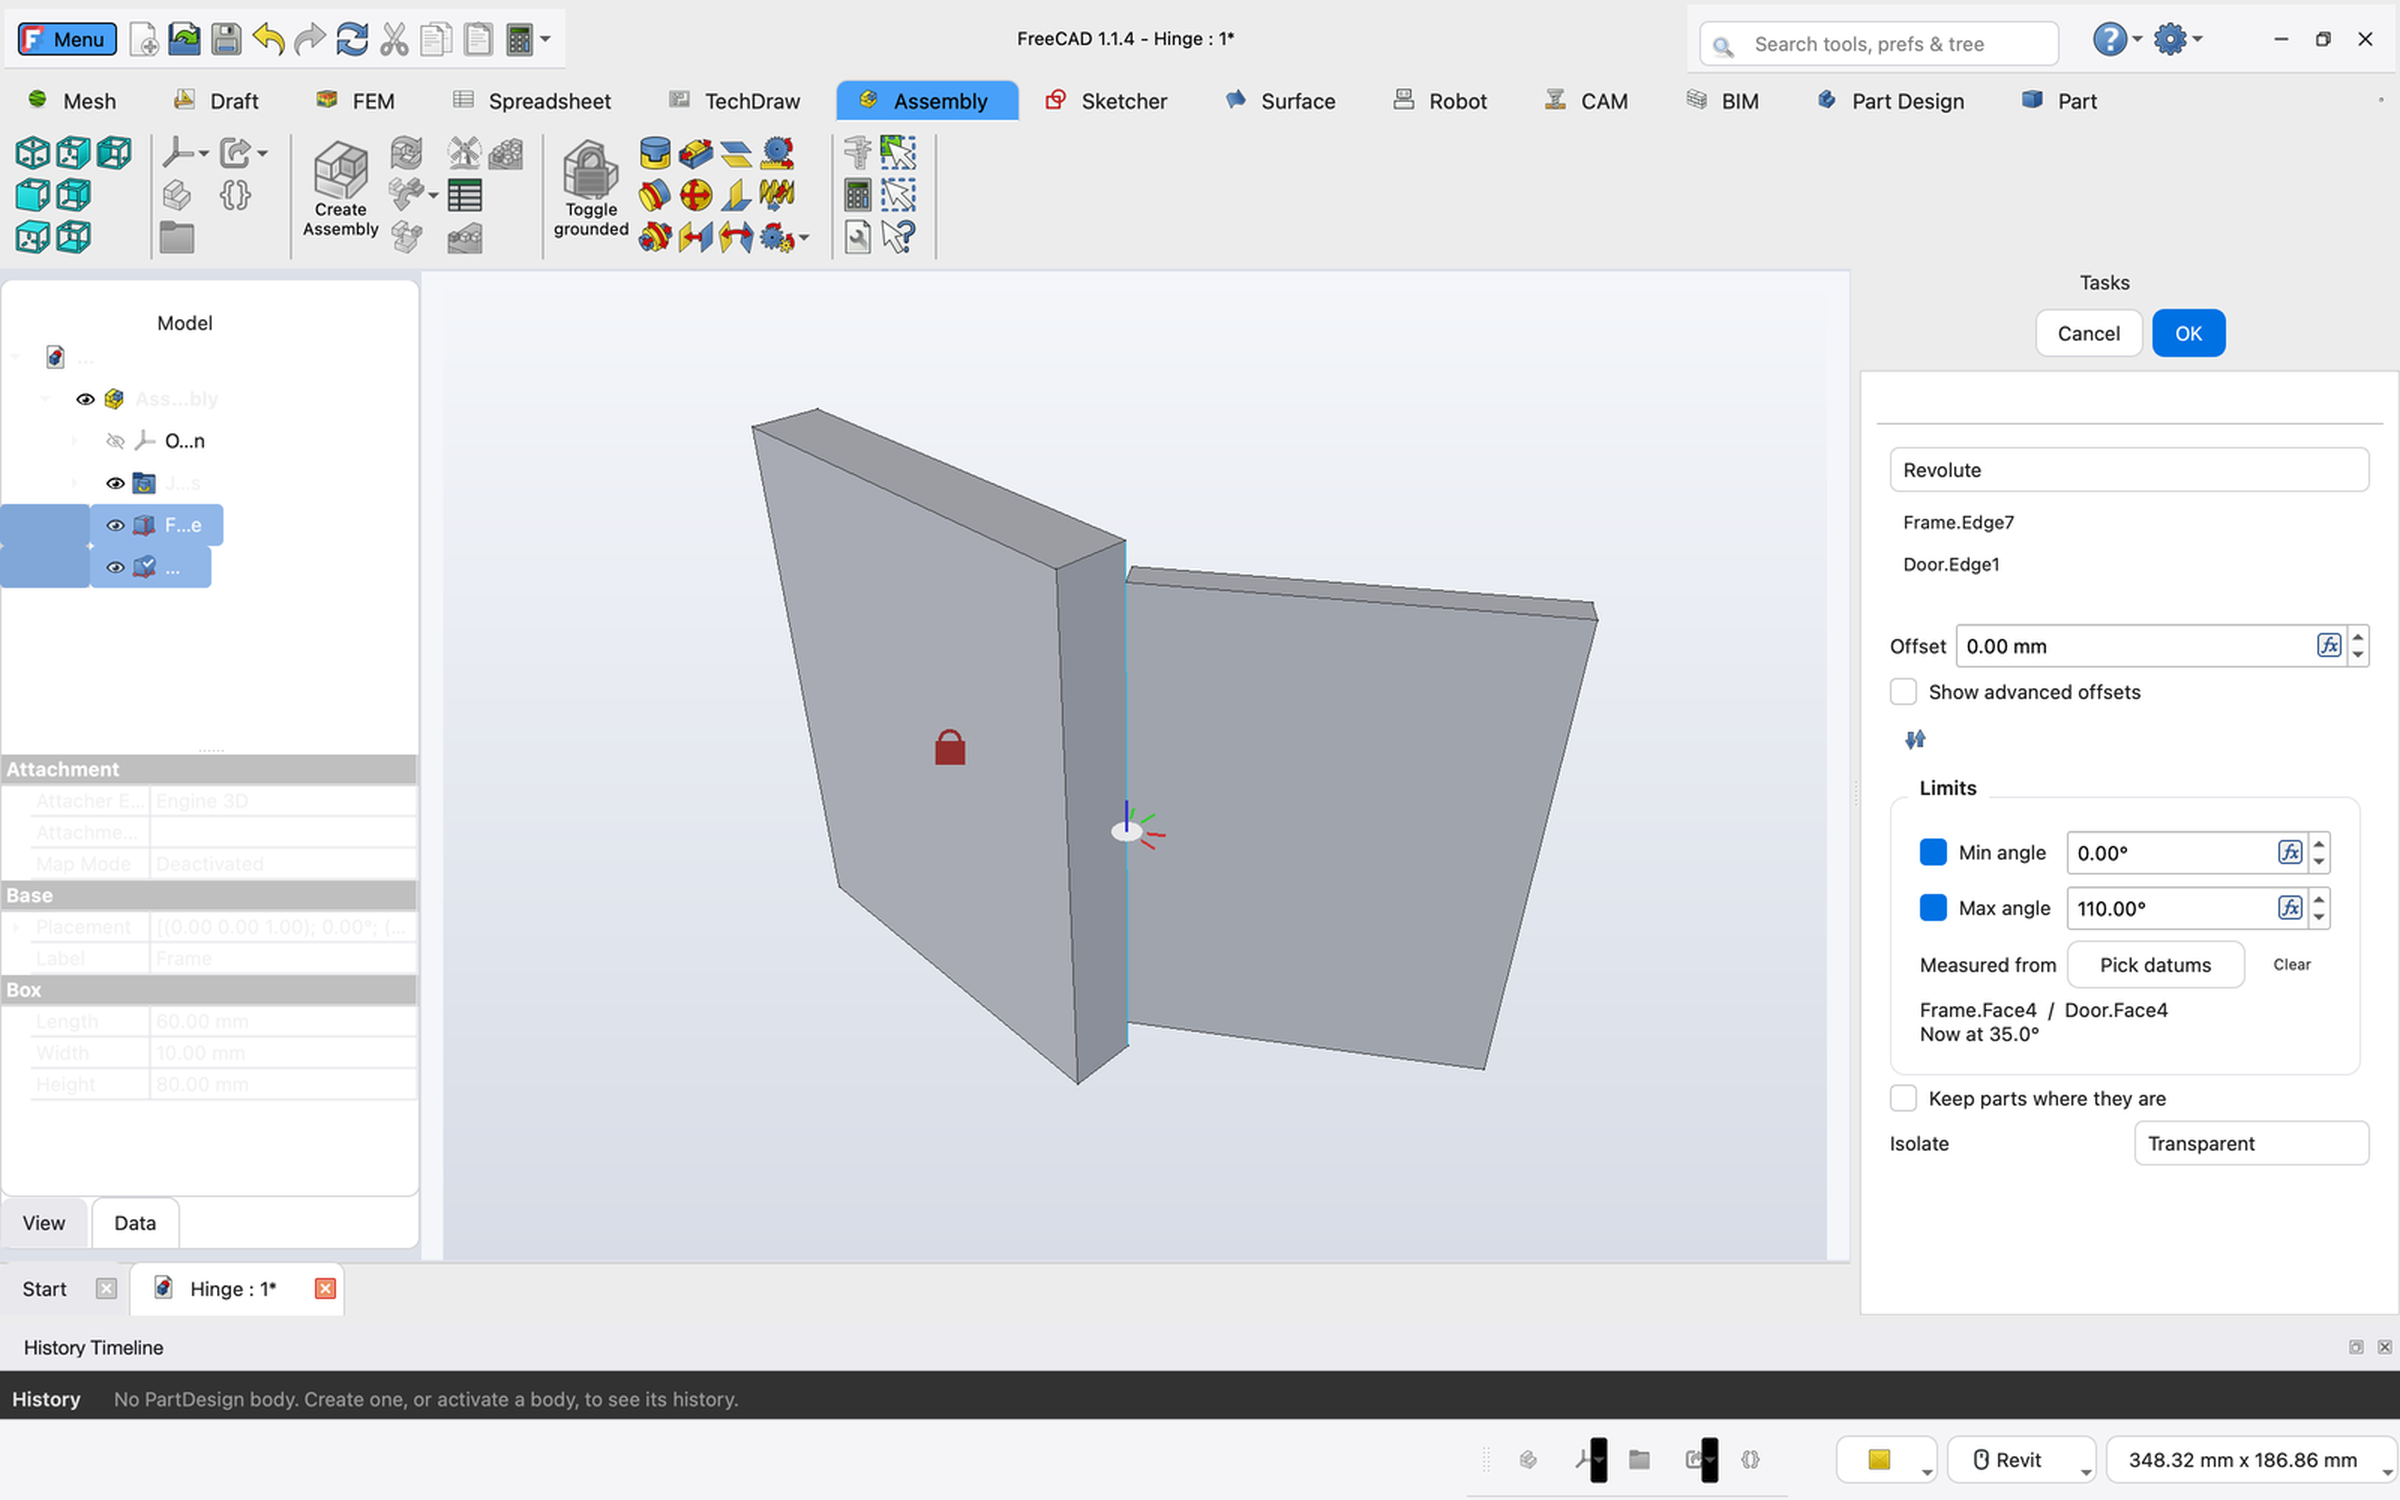
\includegraphics[width=0.497\linewidth]{fig/ui_before_joint.png}\hfill
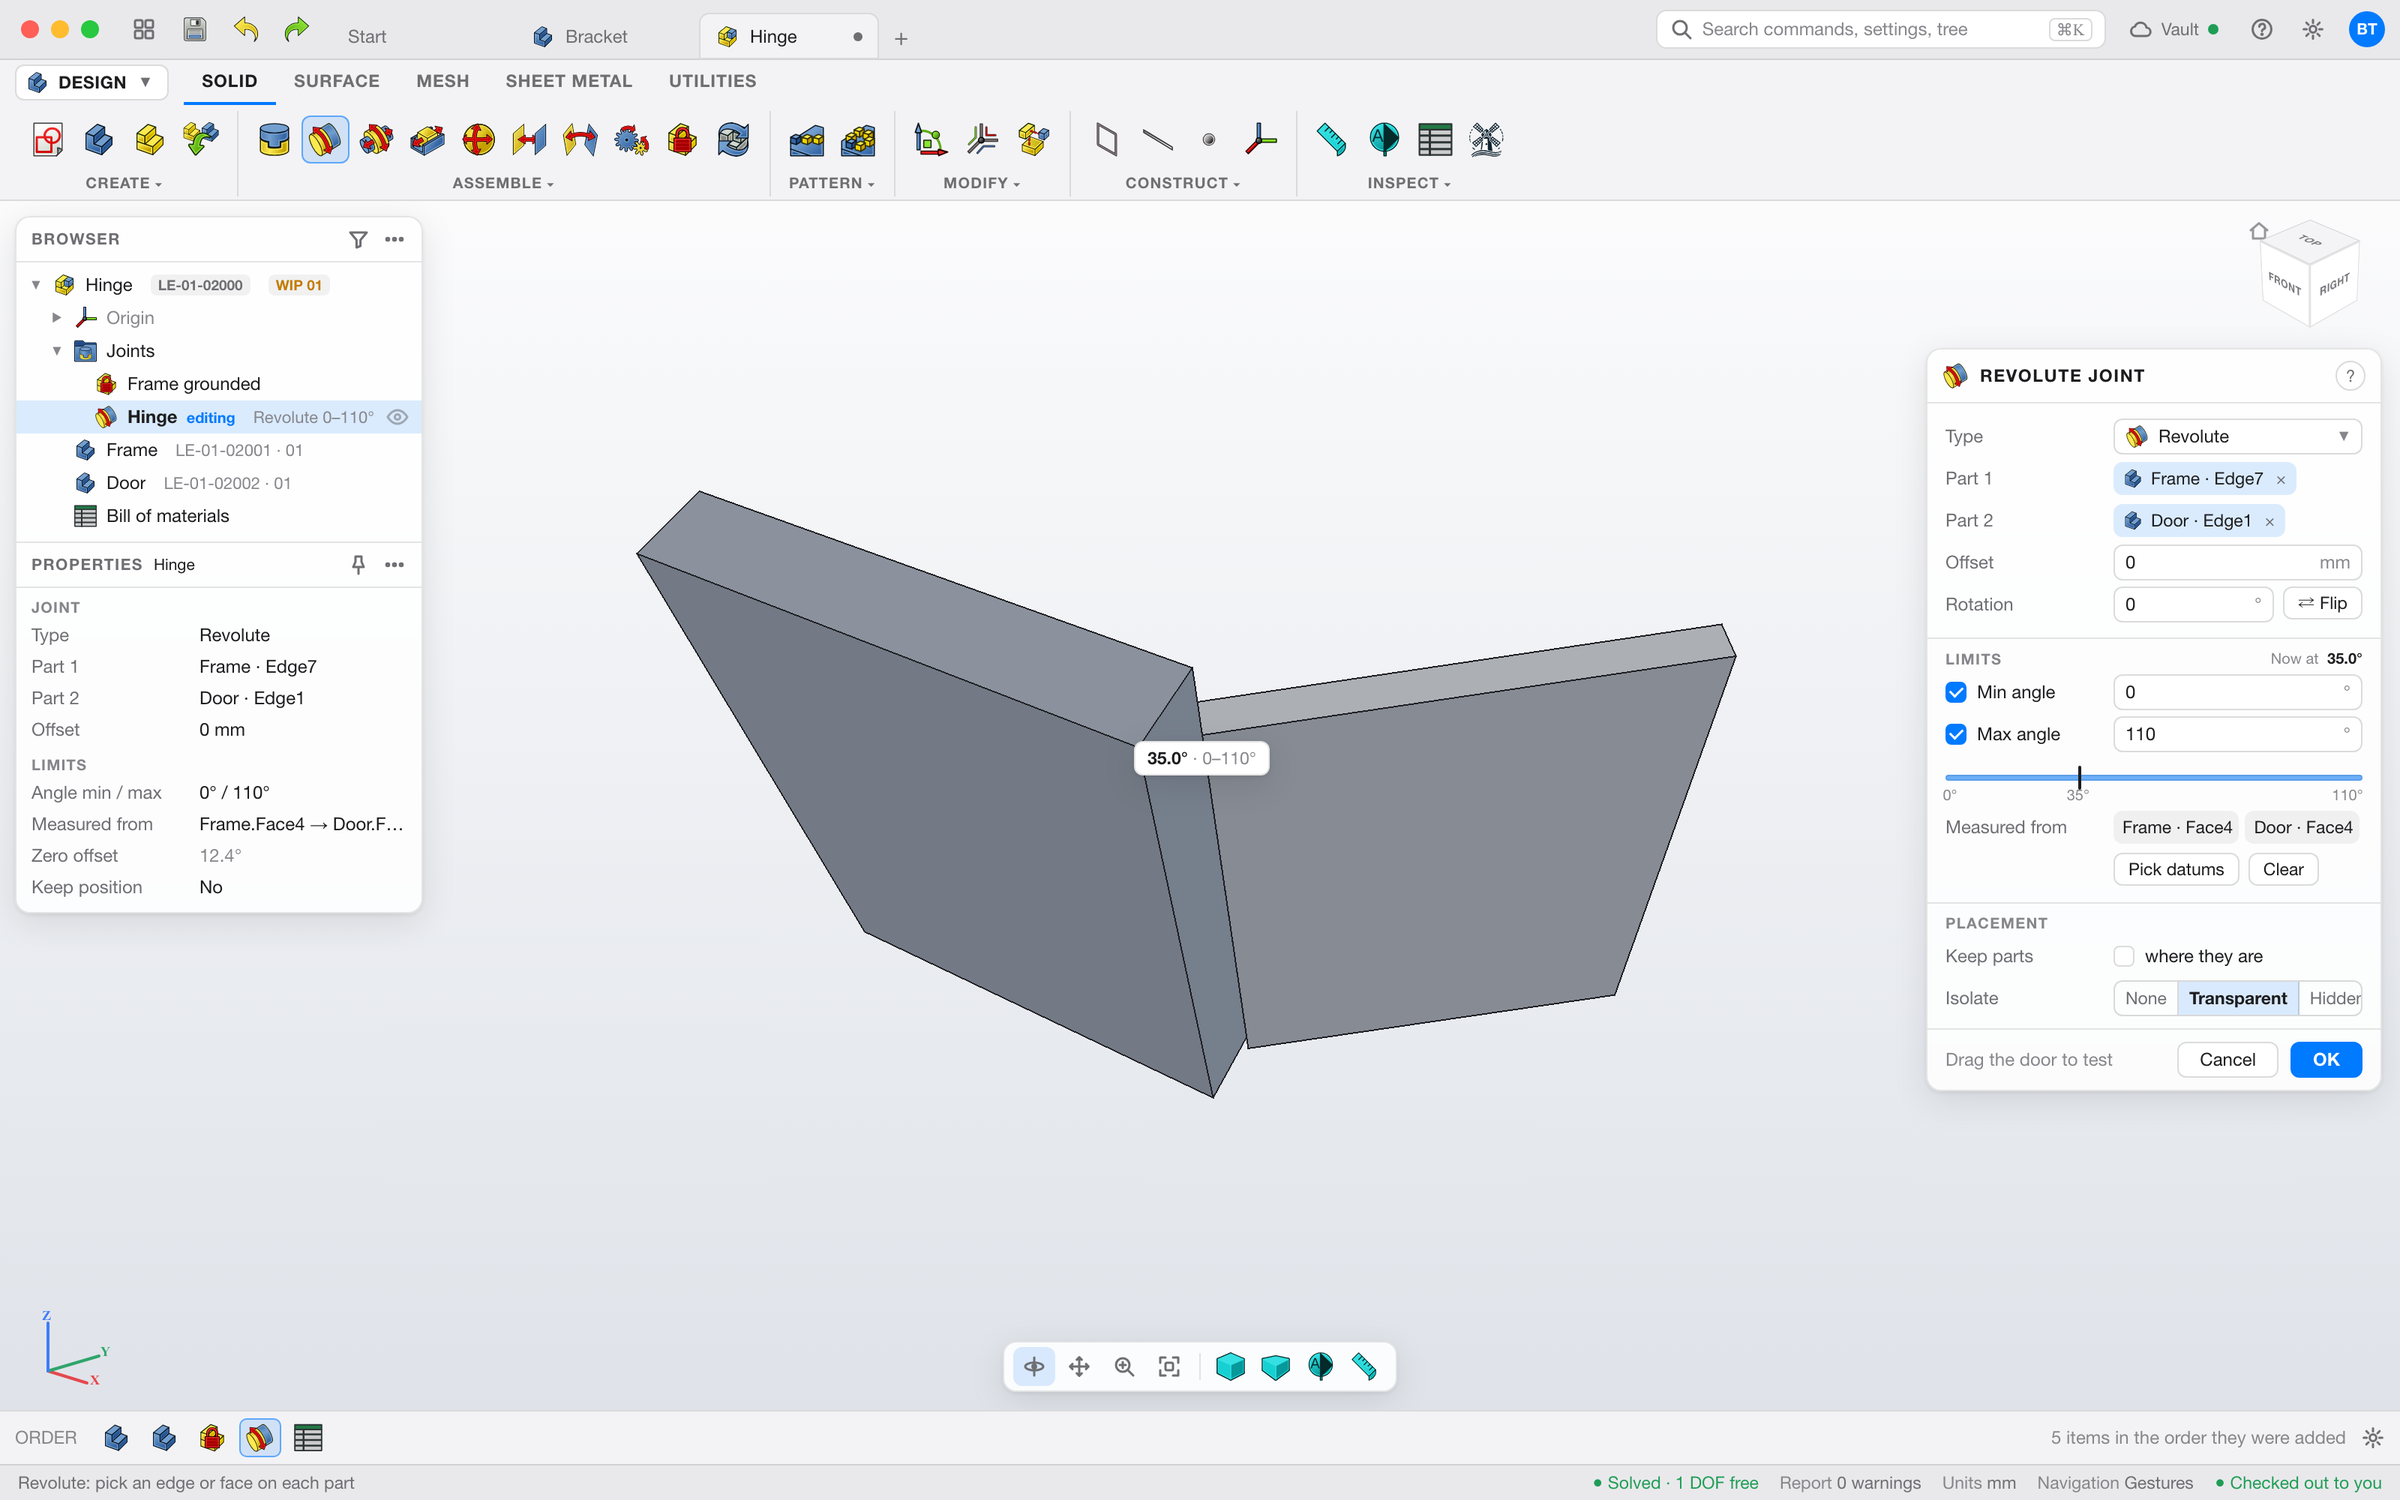
\includegraphics[width=0.497\linewidth]{fig/ui_mock_asm-light.png}
\caption{The same joint, today (left) and in the mock (right).}
\label{fig:ui-before-after}
\end{figure}

\subsubsection*{Plan: three steps, each shown before and after}

Each step ends with the four screens captured from the real build in light and dark, next to these mocks, for you
to approve.

\begin{center}
\small
\begin{tabularx}{\linewidth}{@{}lXl@{}}
\toprule
Step & Work & Size\\
\midrule
\textbf{A. Stylesheet and settings} & Colour tokens and sizes above in \file{BruceWorx.qss} and the two yaml files.
  Cards for Browser and dialog. NaviCube settings. Fix \marker{2}\marker{4}\marker{5}\marker{7}\marker{8}\marker{9}\marker{10}
  of figure~\ref{fig:ui-before}. Ribbon off in the BruceWorx profile. No C++.
  & small\\
\textbf{B. Small code} & Follow appearance and accent (signal + token reload). Document tabs on top. Dialog
  buttons at the bottom. Navigation pill. One-row timeline, hidden without history. Status-bar readouts.
  & medium\\
\textbf{C. Structure} & Workspace menu and tabs (\eref{UIX-05}), captioned groups (\eref{UIX-06}), tabs in the
  title bar, search, Start page, Browser badges. & large\\
\bottomrule
\end{tabularx}
\end{center}

\paragraph{Your answers (19 Oct, second round).}
\begin{enumerate}[nosep]
  \item \textbf{Dark-mode icons:} a faint light plate behind each icon in dark mode only, shown first
        (figure~\ref{fig:ui-plates}). The dark figures above already use it at 10\,\%.
  \item \textbf{Search:} ``yes''. Read as the built-in \texttt{Cmd-K} field; to be confirmed.
  \item \textbf{Ribbon add-on:} my call. BruceWorx turns FreeCAD-Ribbon off in its own profile while the
        BruceWorx bar is on and leaves it installed, so turning the bar off brings Ribbon back.
  \item \textbf{Properties:} stay in the Browser card, which grows down to fit them.
  \item \textbf{Assembly timeline:} components and joints in the order they were added. FreeCAD numbers every
        object as it is created (\code{obj.ID}), so the order needs no new data. No playback buttons:
        an assembly has nothing to roll back.
  \item \textbf{Document tabs:} a thin row under the title bar is acceptable if the title bar is impractical.
\end{enumerate}

\begin{figure}[!htbp]
\centering
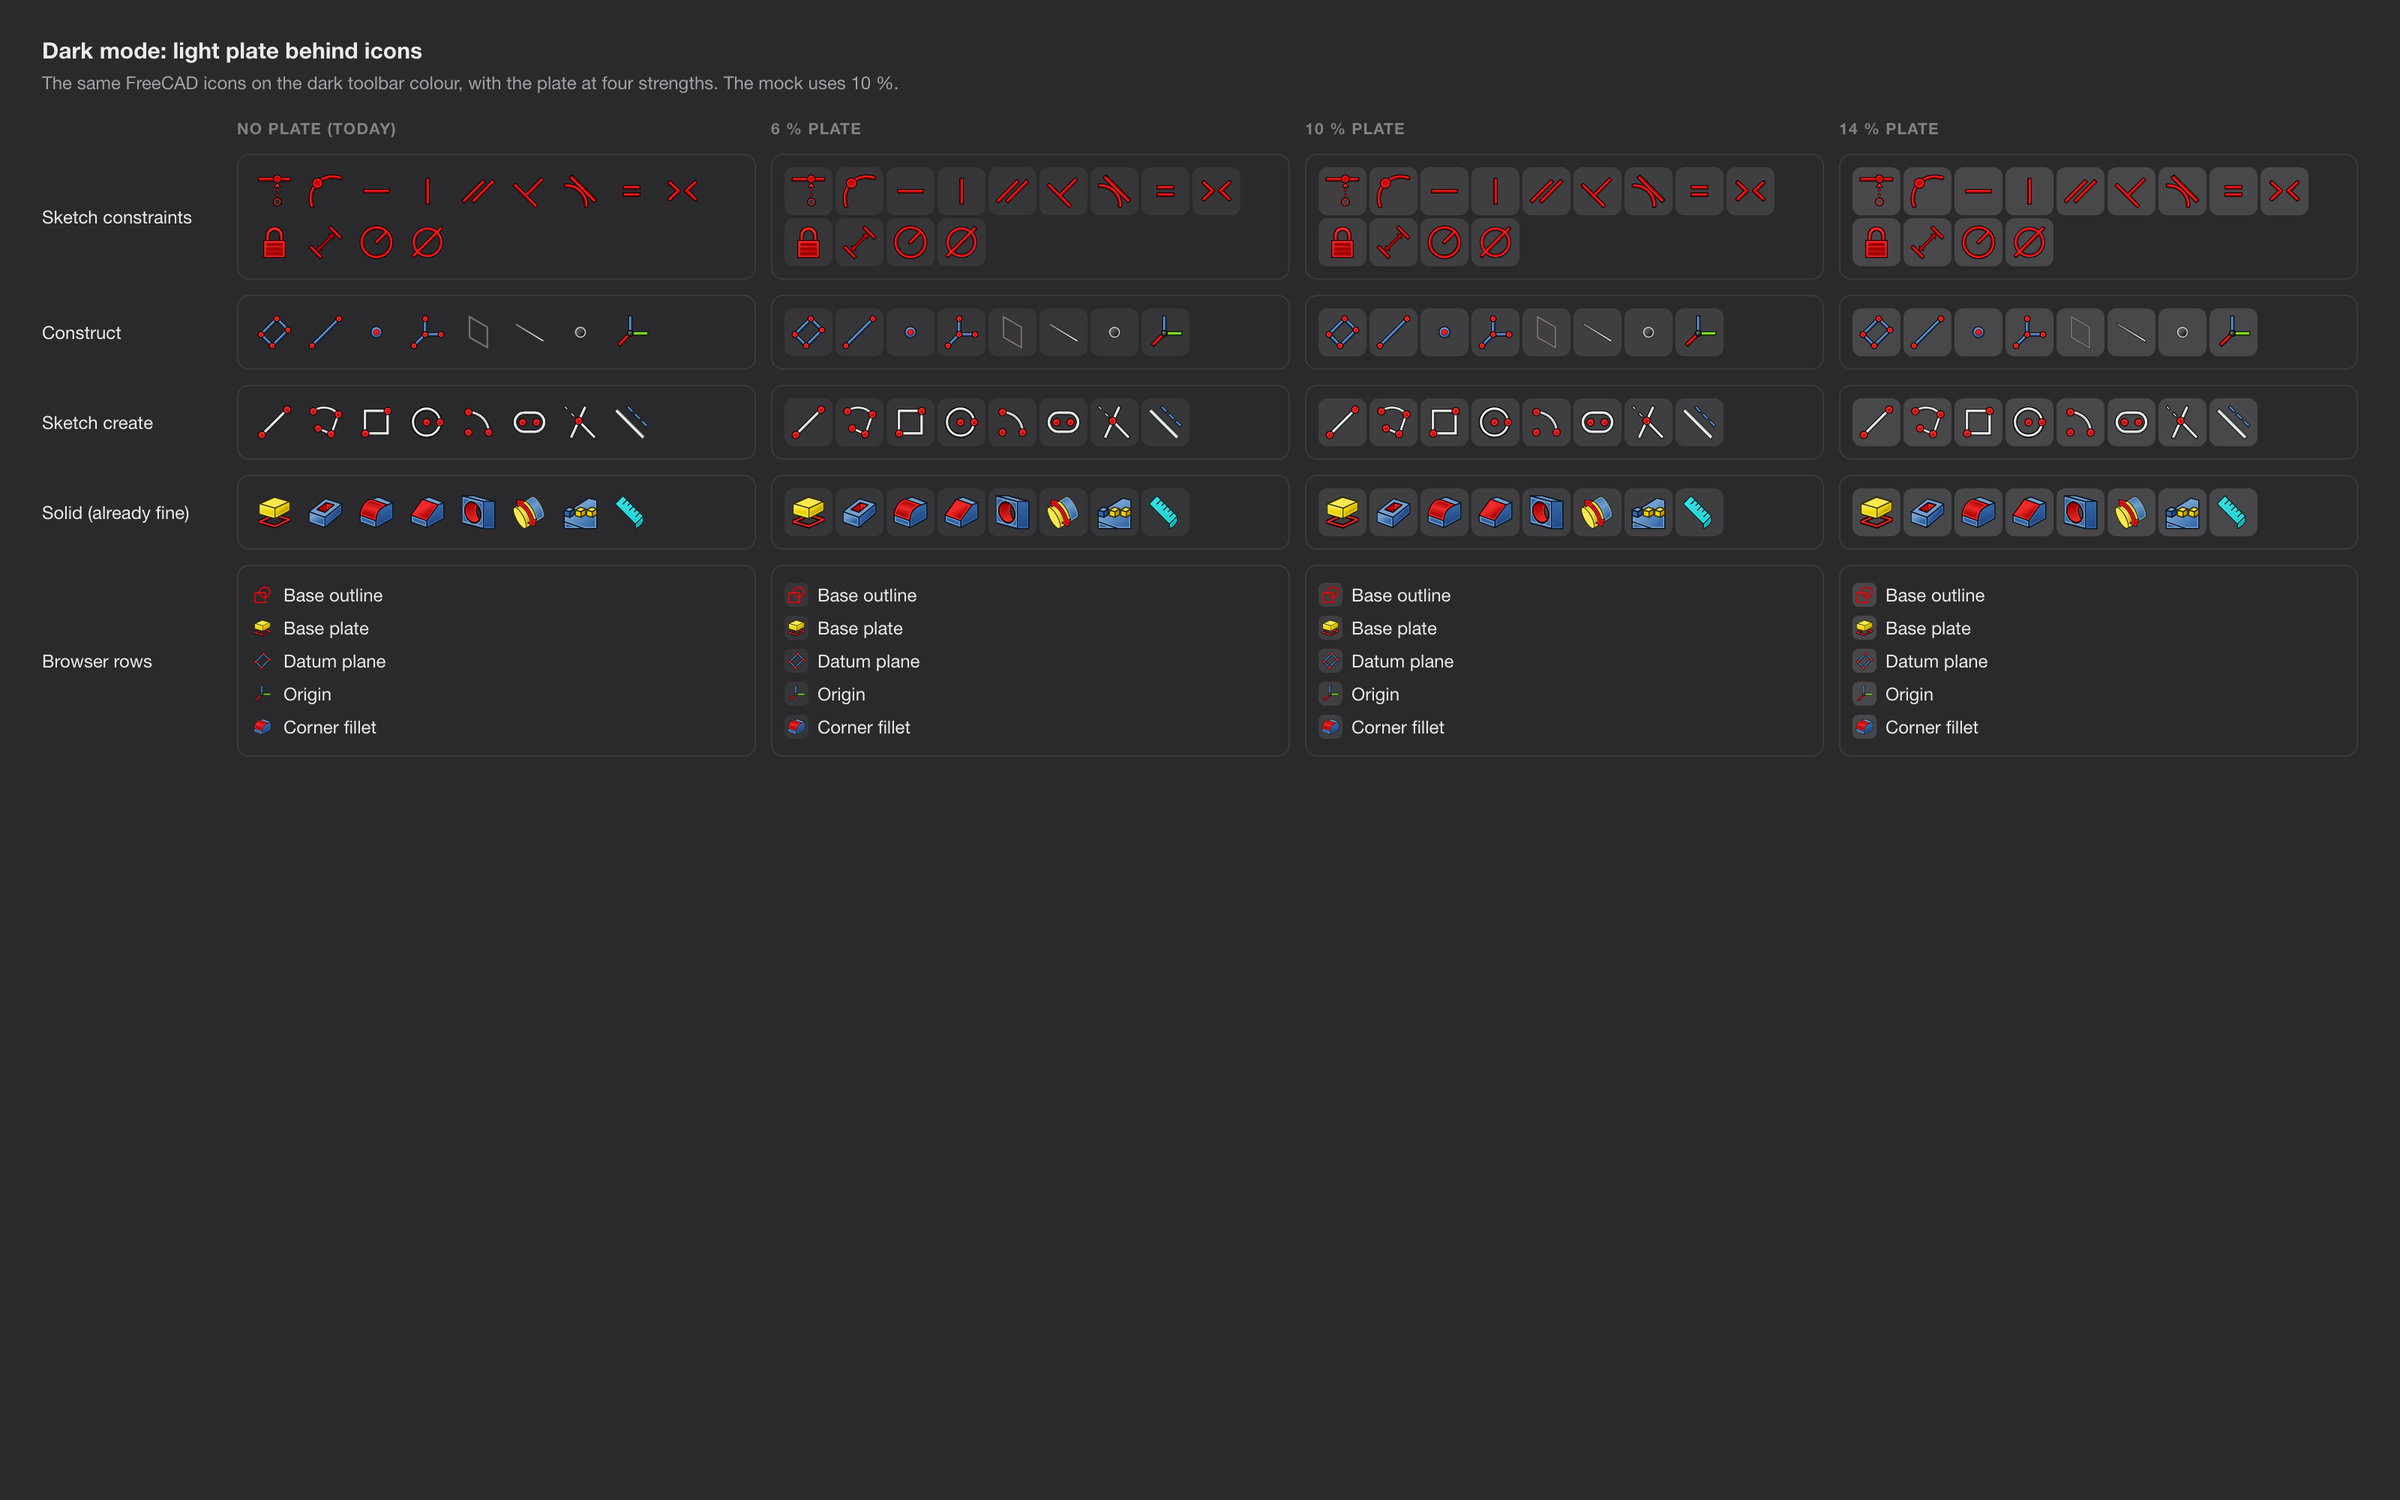
\includegraphics[width=\linewidth]{fig/ui_mock_plates.png}
\caption{Dark mode, the same FreeCAD icons with no plate and with 6, 10 and 14\,\% white plates. The plate lifts
the black-outlined icons (construct, sketch create) clearly. It does much less for the red constraint icons,
whose problem is red on dark rather than outline on dark. In Qt the toolbar plate is one stylesheet rule on the
tool buttons. The plate behind tree and list icons needs a small item delegate (step~B).}
\label{fig:ui-plates}
\end{figure}

\subsubsection*{Step A: done (19 Oct 2026)}

\begin{figure}[!htbp]
\centering
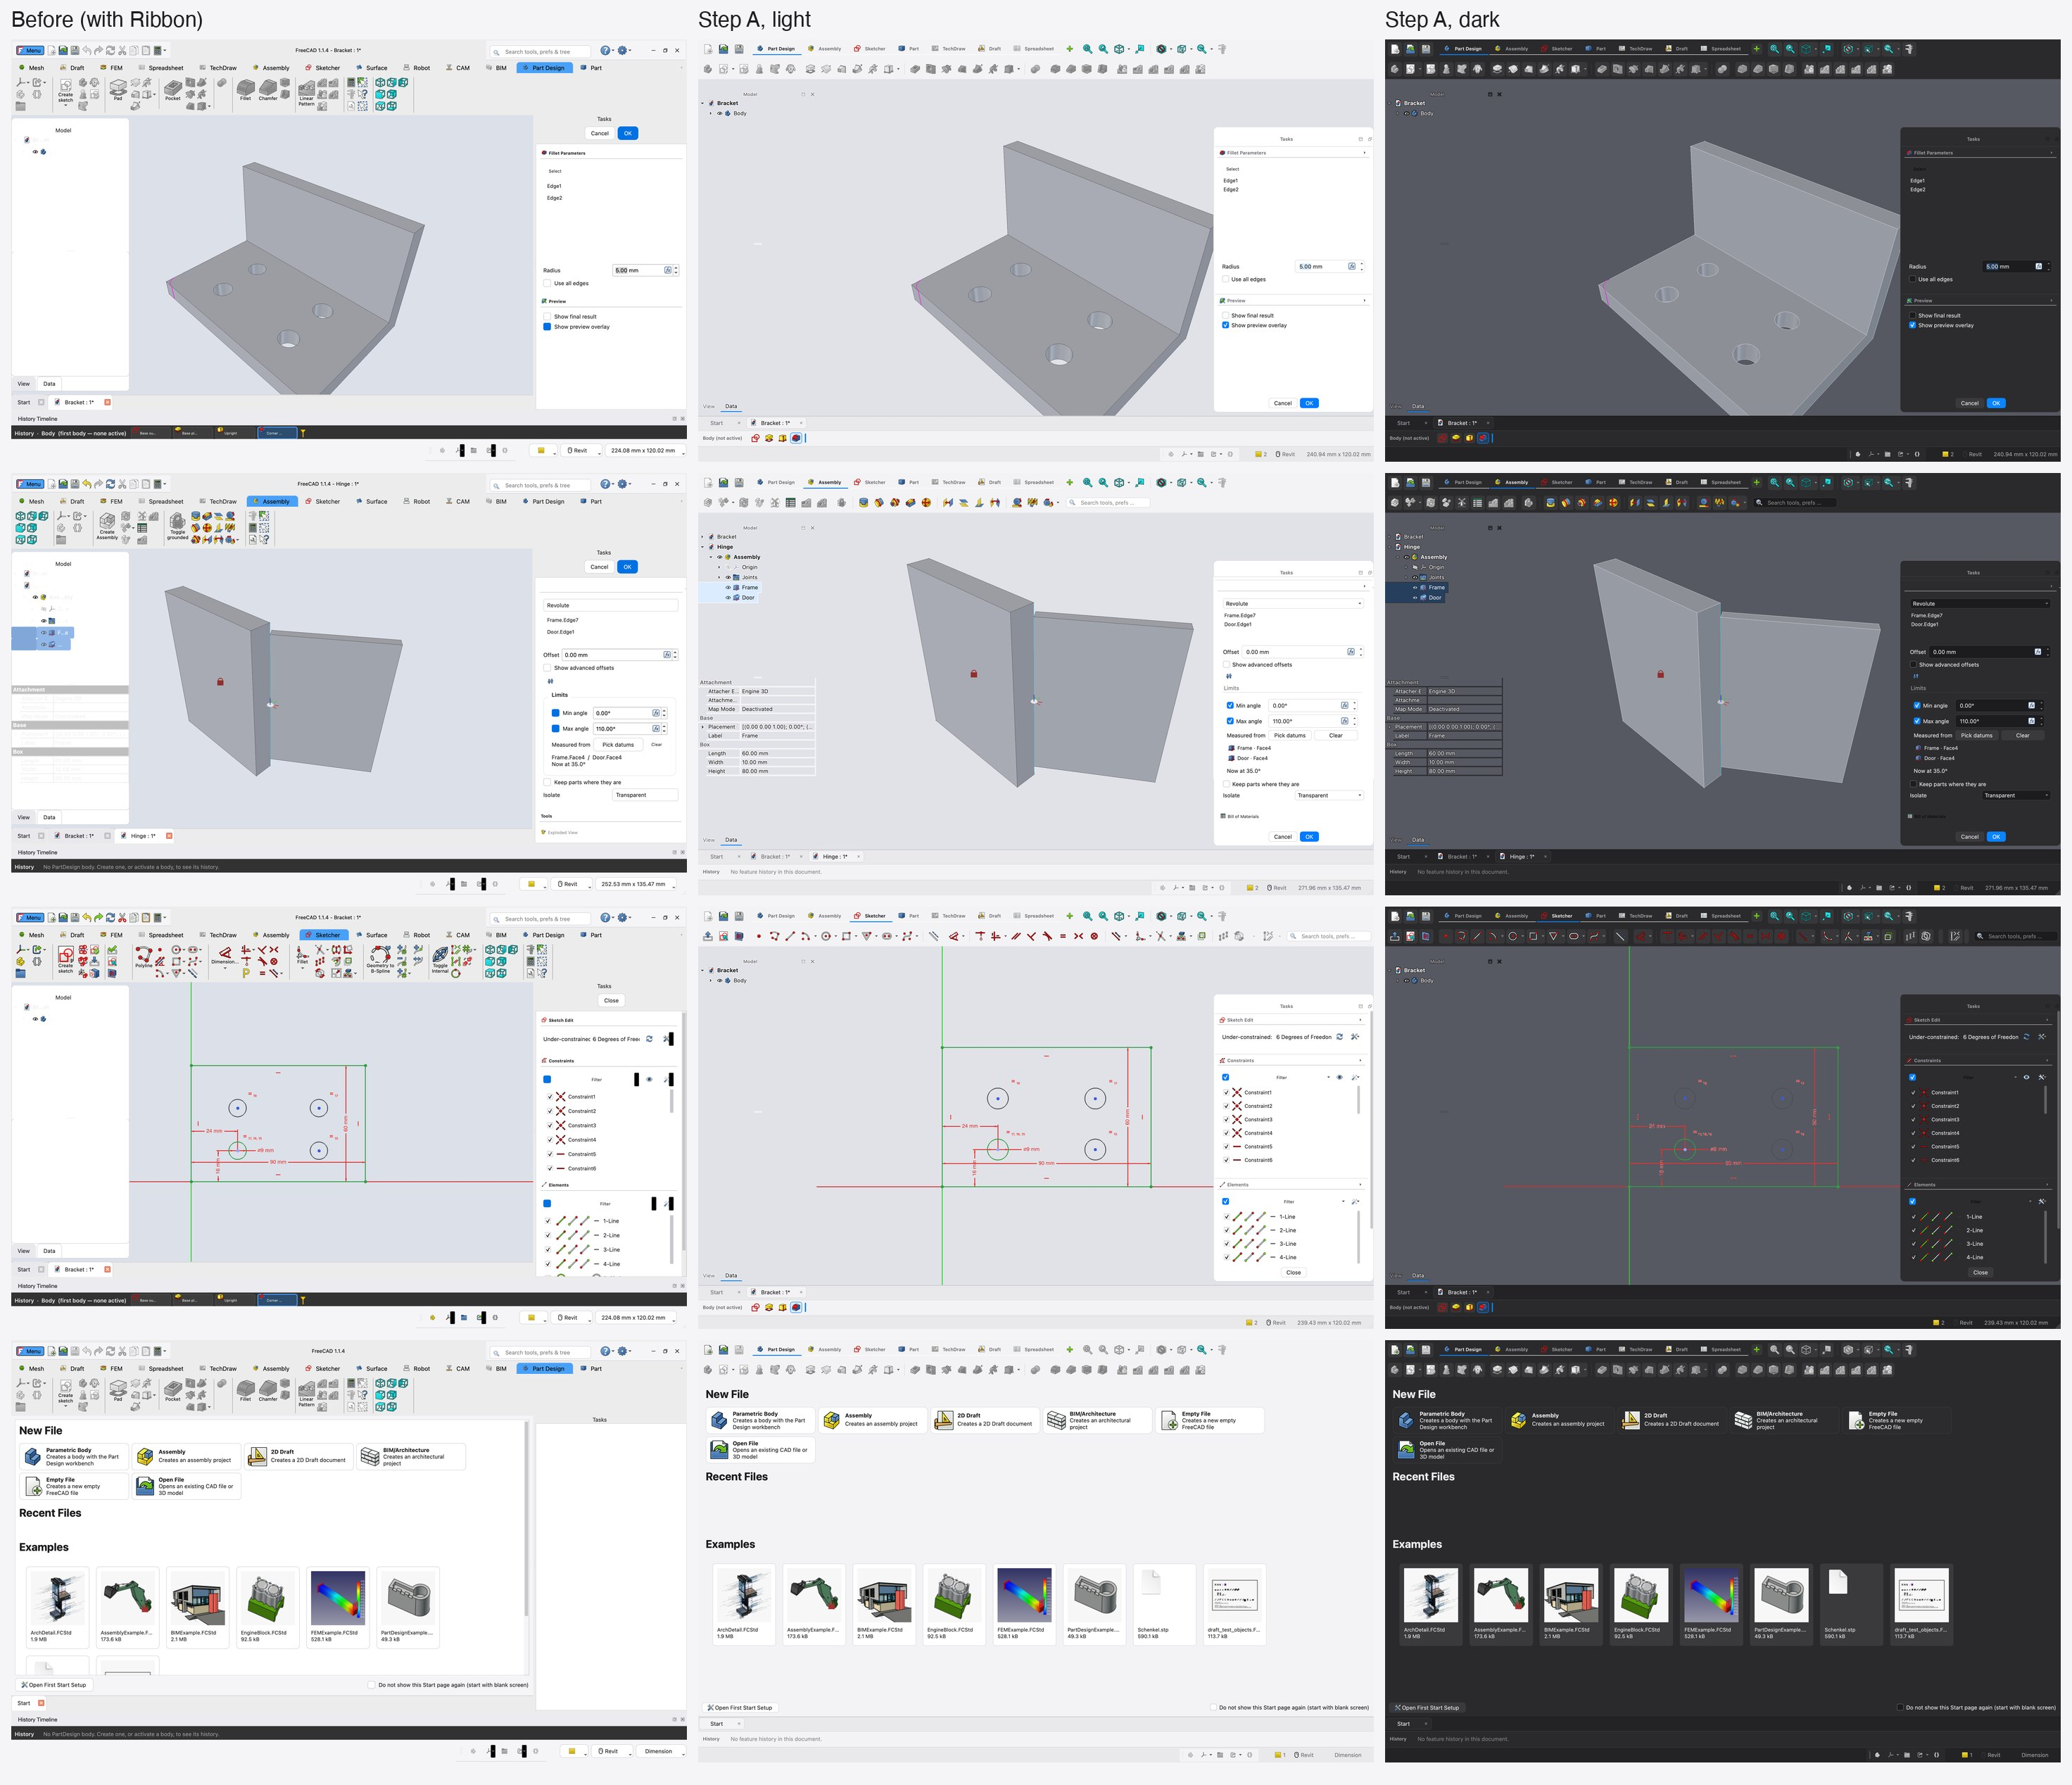
\includegraphics[width=\linewidth]{fig/ui_stepA_sheet.jpg}
\caption{The real build, captured on a copy of your settings: before (Ribbon on), and after step A in light
and dark. Rows: part with a fillet open, the hinge joint, a sketch, the Start page. The 3D view is rendered
separately and pasted in, because a window grab leaves it blank; the view cube is not in these pictures.}
\label{fig:ui-stepA}
\end{figure}

\begin{center}
\small
\begin{tabularx}{\linewidth}{@{}X>{\raggedright\arraybackslash}p{5.1cm}@{}}
\toprule
Change & Where\\
\midrule
Colour tokens from the mock, light and dark; \code{blend()} gives the soft accent & \file{parameters/BruceWorx*.yaml}\\
12\,px type, 22\,px rows, 6/10\,px corners, flat task boxes as cards, thin tab $\times$ & \file{BruceWorx.qss}, \file{close-thin-*.svg}\\
Tree names no longer cut short (horizontal item padding removed) & \file{BruceWorx.qss}\\
Checkboxes show a tick; drop-down tools no longer paint a black bar & \file{BruceWorx.qss}\\
Dark-mode icon plate, 6\,\% white mixed into the toolbar colour (tokens carry no alpha) & \file{BruceWorx Dark.yaml}\\
Browser slightly transparent (your choice): a tinted glass card, 72\,\% opaque, text with a halo & \file{BruceWorx.py}, \file{BruceWorxModelTree.qss}\\
Task panel floats right as one card, shown only while a command is open; its boxes are flat sections & \file{BruceWorx.py}, \file{BruceWorxModelTree.qss}\\
OK/Cancel at the foot of every task panel (dialogs that choose a side keep it) & \file{TaskDialog.cpp}\\
Picks shown as lists: limit datums (Delete removes one), pattern objects & \file{JointObject.py}, \file{bruceworx\_pattern\_gui.py}\\
FreeCAD-Ribbon not loaded while \emph{BruceWorx top bar} is on (stays installed; stock FreeCAD still loads it) & \file{FreeCADInit.py}, \file{FreeCADGuiInit.py}\\
Two toolbar rows after every workbench switch (stale line breaks gave three or four) & \file{bruceworx\_toolbars.py}\\
Timeline: one row of icon chips in theme colours, no dock title, quiet empty message & HistoryTimeline mod\\
Start page readable in dark & \file{BruceWorx.qss}\\
Viewport gradient, accent, selection and view-cube colours from the mock & \file{bruceworx\_pack.py} (cfg regenerated)\\
Sketch grid on, as in the mock (your pick): faint translucent lines (white on dark, black on light), a major line every 5 squares, follows the zoom. The grid now honours a colour's alpha & \file{bruceworx\_pack.py}, \file{ViewProvider\-Grid\-Extension.cpp}\\
\emph{Sketch grid strength} preference, 2--40\,\%, default 10; open sketches update at once. Python: \code{bruceworx\_grid.set\_strength(14)}; a \code{GRID 14} alias comes with the command line (\eref{AUT-05}) & \file{bruceworx\_grid.py}\\
Joint panel \emph{Clear} is a normal button & \file{TaskAssemblyCreateJoint.ui}\\
\bottomrule
\end{tabularx}
\end{center}

New switches on Preferences $\rightarrow$ BruceWorx, all on by default: \emph{BruceWorx top bar}, \emph{Two
toolbar rows}, \emph{Float the task panel}; \emph{Transparent background} is on again by default. OK/Cancel at the
bottom reads \code{BruceWorx/TaskButtonsAtBottom} (no checkbox yet). Tests: 10 BruceWorx, 19 pattern, 16 Assembly, 26 pack, all passing.
To see the new colours on your own profile the pack must be applied again (Preferences $\rightarrow$ General
$\rightarrow$ Preference packs $\rightarrow$ BruceWorx), because a pack writes its values once.

\paragraph{Found on the way.} Editing a \file{.ui} panel does not rebuild the module's \file{\_rc.py}: the build
only watches the \file{.qrc}, and Python loads panels from that file. That was the cause of the stale joint
panel earlier today too. Until the CMake rule is fixed, delete \file{build/release/\{src/Mod/X/Gui,Mod/X\}/X\_rc.py}
after changing a panel.

\paragraph{Left for step B.} Task card header with the command's icon and title (a box without a title still
shows an empty strip); an inset from the right window edge (the overlay pins panels to the edge);
\textsc{Browser} header and badges; navigation pill; timeline in creation order for assemblies and hidden when
there is no history; follow the macOS appearance and accent live; sketch colours (free geometry blue,
constrained in text colour, dimensions quiet); document tabs on top; the property group captions.

\subsubsection*{Step B, in progress}

\paragraph{1. Follow macOS appearance and accent (done).} \file{bruceworx\_appearance.py} listens for Qt's
\code{colorSchemeChanged} and for palette or activation events (macOS has no accent signal). On a light/dark
change it writes only the pack values that differ between the two modes; FreeCAD reloads the stylesheet when the
Theme parameter changes. The accent is read from \code{AppleAccentColor} and written to
\code{ThemeAccentColor1}, which the yaml files now use as \code{@AccentColor}, and to the 3D selection and
view-cube highlight. Text and ticks on the accent follow the contrast rule above: verified live, a yellow
accent gets dark text and dark ticks, blue gets white. Two switches on Preferences $\rightarrow$ BruceWorx, both on.
Theme tokens from \emph{Themes/UserParameters} take precedence over the yaml, so the computed
\code{AccentTextColor} wins over the yaml default.

%======================================================================
\section{Track KRN --- Kernel study (background)}\label{sec:krn}
%======================================================================

A study, not a build. It answers what it would cost to put FreeCAD on a different geometry kernel, without
blocking any parity work.

\begin{epic}{KRN-01}{OCCT coupling survey}{BG}{\stTodo}{FCB-P3-01..06}
Script-count OCCT includes and call sites per module (Part, PartDesign, Sketcher, TechDraw, Surface, FEM,
CAM). Analyse the topological-naming and element-map dependencies (\code{TopoShapeExpansion},
\code{ShapeMapper}, \code{ElementMap}) and how far OCCT leaks into Python bindings. Write option A (a
facade over \code{TopoShape}) as a design note.
\end{epic}

\begin{epic}{KRN-02}{STEP exchange harness}{BG}{\stTodo}{FCB-P3-07..11}
A separate harness repository: LE corpus STEP files (shared with \eref{FND-05}), round-trip metrics
(volume, bounding box, face and edge counts, validity), a minimal kernel stub that reads and writes primitives,
and Linux CI.
\end{epic}

\begin{epic}{KRN-03}{Kernel decision}{BG}{\stTodo}{FCB-P3-12/13/14}
An A/B/C memo with effort estimates, reviewed, then a gate. Nothing in tracks MOD--MFG waits on it. The
parity work uses \code{TopoShape} APIs, so it carries over under option A.
\end{epic}

%======================================================================
\section{Open questions}\label{sec:questions}
%======================================================================

These are decisions the roadmap cannot make for you. None of them blocks M0. Each lists the epic it gates.

\begin{enumerate}[label=Q\arabic*.,ref=Q\arabic*]
  \item\label{q:fct01} \textbf{FC-T01 switch criteria} (\eref{PDM-08}, M6). The Ops data shows the gate
        ``Bruce sets FC-T01 switch criteria'' as done, but the criteria aren't recorded. What are they? They
        become M6's checklist and the scope filter on the parity matrix.
  \item\label{q:cfgpn} \textbf{Part numbers for configurations} (\eref{MOD-03}). Proposed: each configuration
        that is manufactured separately gets its own P/N (\S\ref{sec:mod}). Or should variants share a P/N with
        a dash suffix?
  \item\label{q:dwgpn} \textbf{Drawing numbers} (\eref{PDM-02}, \eref{DRW-01}). Is a drawing its own item with
        a document-type code (\code{\{DT\}}) different from its part, or does it share the part's P/N? Their
        revisions move together either way.
  \item\label{q:cnc} \textbf{CNC machine and controller} (\eref{MFG-02}). Which machine(s) and controller
        (GRBL, LinuxCNC, Haas, \ldots)? This picks the post-processor and the tool library.
  \item\label{q:openscad} \textbf{OpenSCAD binary} (\eref{AUT-05}). Ship the official OpenSCAD app (GPL-2, as a
        separate executable) in the DMG, or require a user install with a hint?
  \item\label{q:compute} \textbf{Pattern Compute: Adjust} (\eref{MOD-01}). OK to ship \emph{Identical} only
        and add \emph{Adjust} later?
  \item \textbf{Joints on patterned components} (\eref{MOD-01}). Leave instances free, like Fusion, or
        copy the seed's joints?
  \item \textbf{Upstreaming} (\eref{FND-03}). With upstream main tracked continuously, should generic fixes
        (like \code{Spacings2}) and small core patches go upstream by default to shrink the conflict budget?
  \item \textbf{Fastener library} (\eref{MOD-05}). Adopt the FreeCAD Fasteners add-on if its licence fits, or
        build on the COTS schema only?
  \item \textbf{PDM evaluation weights} (\eref{PDM-01}). Confirm or change the proposed weights in
        \S\ref{sec:pdm}.
  \item \textbf{ECAD bridge decision} (\eref{ECD-01}). Was ``adopt StepUp vs build'' decided (it shows as done in the
        sample data)? If so, which way?
  \item \textbf{FDM knockdown factors} (\eref{SIM-03}). Run coupon tests on our printers and materials, or start
        from published values?
  \item \textbf{Command aliases} (\eref{AUT-05}). Start from AutoCAD names (\code{EXT}, \code{F}, \code{AR}) or
        Fusion's single keys (\code{E}, \code{F}, \code{H})?
  \item \textbf{Distribution} (\eref{FND-02}). Will anyone outside the team install builds before M6? If so,
        signing and notarisation move into M0.
\end{enumerate}


\appendix
%======================================================================
\section{Parity matrix}\label{app:parity}
%======================================================================

\pfull{} full \quad \phalf{} partial \quad \pnone{} none \quad \padd{} add-on only. Fusion = Fusion~360 with
its extensions, SW = SolidWorks 2026 (Premium/PDM/Simulation), both from public vendor and reseller material
(Oct 2026). A cell marked † is the vendor capability we could not confirm from that material. The FreeCAD column is
\emph{1.1.4 as built in this repository}, with the evidence found in \file{src/} or by headless experiment.
``Out of scope'' rows were not selected in the interview and have no epic.

\begin{center}
\small
\begin{longtable}{@{}p{4.2cm}ccc p{5.6cm} p{1.5cm}@{}}
\toprule
Capability & Fusion & SW & FC & FreeCAD evidence / note & Epic\\
\midrule\endhead
\bottomrule\endfoot
\multicolumn{6}{@{}l}{\textbf{Sketch and part}}\\
Parametric sketch \& constraints & \pfull & \pfull & \pfull & Sketcher & MOD-12\\
Extrude, revolve, sweep, loft & \pfull & \pfull & \pfull & PartDesign & ---\\
Fillet, chamfer, shell, draft & \pfull & \pfull & \pfull & PartDesign & ---\\
Hole wizard / presets & \pfull & \pfull & \phalf & \code{Hole} feature; no insert presets & MOD-05\\
Cosmetic threads & \pfull & \pfull & \phalf & TechDraw view extension only & MOD-05\\
Feature patterns & \pfull & \pfull & \phalf & \code{LinearPattern} dir.-2 bug; no symmetric/suppress & MOD-01\\
Body / component patterns & \pfull & \pfull & \phalf & Draft link arrays, not assembly-aware & MOD-01\\
Parameters dialog & \pfull & \pfull & \phalf & Spreadsheet, \code{VarSet}, expressions & MOD-02\\
Configurations / design tables & \pfull & \pfull & \pnone & none found in Spreadsheet or App & MOD-03\\
Multi-body, derive, skeleton & \pfull & \pfull & \phalf & \code{SubShapeBinder} cross-document & MOD-02\\
Direct edit (press-pull, move face) & \pfull & \pfull & \phalf & \code{Part\_Defeaturing} only (verified) & MOD-04\\
Surfacing (patch, trim, stitch) & \pfull & \pfull & \phalf & Surface WB: Filling, Sections, Extend, Blend & MOD-08\\
Continuity / zebra analysis & \pfull & \pfull & \pnone & --- & MOD-08\\
Freeform / T-spline & \pfull & \phalf & \pnone & --- & MOD-09\\
Mesh $\rightarrow$ B-rep & \pfull & \pfull & \phalf & \code{Part\_ShapeFromMesh} (faceted), ReverseEngineering & MOD-10\\
Sheet metal & \pfull & \pfull & \padd & SheetMetal add-on (to bundle) & MOD-06\\
Weldments / frames & \phalf† & \pfull & \pnone & --- & MOD-07\\
Plastic features (rib, boss, snap) & \pfull & \pfull & \pnone & out of scope (no molding) & ---\\
Measure & \pfull & \pfull & \pfull & Measure WB & ---\\
Mass properties & \pfull & \pfull & \phalf & \code{MeasureCOM}; no inertia report & MOD-11\\
Section analysis & \pfull & \pfull & \phalf & clipping / section cut & MOD-11\\
Draft / overhang analysis & \pfull & \pfull & \pnone & --- & MOD-11\\
Wall-thickness analysis & \phalf† & \pfull & \pnone & --- & MOD-11\\
\midrule
\multicolumn{6}{@{}l}{\textbf{Assembly}}\\
Joints / mates & \pfull & \pfull & \pfull & Assembly WB (Ondsel solver) & ASM-03\\
Joint limits while dragging & \pfull & \pfull & \phalf & limit properties exist; drag to check & ASM-03\\
Rigid / flexible sub-assemblies & \pfull & \pfull & \phalf & to audit & ASM-05\\
Exploded views & \pfull & \pfull & \pfull & \code{Assembly\_CreateView} & ASM-04\\
BOM (indented, flattened, props) & \pfull & \pfull & \phalf & 4 auto columns + custom & ASM-04\\
Interference / clearance & \pfull & \pfull & \pnone & no command found & ASM-06\\
In-context editing & \pfull & \pfull & \phalf & \code{SubShapeBinder} & ASM-07\\
Large-assembly mode & \phalf & \pfull & \pnone & no lightweight mode found & ASM-08\\
Smart fasteners & \phalf† & \pfull & \pnone & --- & ASM-09\\
Standard-parts library & \pfull & \pfull & \padd & Fasteners add-on & MOD-05\\
Kinematic motion & \pfull & \pfull & \pfull & \code{Assembly\_CreateSimulation} (1.1) & ROB-05\\
Dynamic motion & \phalf & \pfull & \pnone & solver dynamics not exposed & ASM-10\\
\midrule
\multicolumn{6}{@{}l}{\textbf{Simulation}}\\
Linear static & \pfull & \pfull & \pfull & CalculiX \code{static} & SIM-01\\
Contact \& bolts & \pfull & \pfull & \phalf & contact (1.1); no bolt connector & SIM-02\\
Modal & \pfull & \pfull & \pfull & CalculiX \code{frequency} & SIM-01\\
Buckling & \pfull & \pfull & \pfull & CalculiX \code{buckling} & SIM-01\\
Thermal / thermal stress & \pfull & \pfull & \pfull & \code{thermomech}, Elmer & SIM-01\\
Study setup UX & \pfull & \pfull & \phalf & FEM WB, manual & SIM-01\\
Safety-factor result & \pfull & \pfull & \pnone & none in \code{femresult} & SIM-04\\
Orthotropic materials & \phalf† & \pfull & \pnone & none in \file{src/Mod/Fem} & SIM-03\\
Nonlinear / event & \pfull & \pfull & \phalf & out of scope & ---\\
Fatigue & \pnone† & \pfull & \pnone & out of scope & ---\\
CFD & \phalf & \pfull & \phalf & Elmer flow; CfdOF add-on & SIM-06\\
Generative / topology & \pfull & \phalf & \pnone & out of scope & ---\\
\midrule
\multicolumn{6}{@{}l}{\textbf{Drawings}}\\
Projected, section, detail, broken & \pfull & \pfull & \pfull & TechDraw & DRW-06\\
Dimensions incl.\ ordinate/chain & \pfull & \pfull & \pfull & TechDraw + extensions & ---\\
GD\&T (semantic) & \pfull & \pfull & \phalf & SVG symbol library only & DRW-03\\
Hole \& thread callouts & \pfull & \pfull & \phalf & drawing-side extension & DRW-04\\
Parts list + balloons & \pfull & \pfull & \phalf & balloons; spreadsheet view & DRW-02\\
Revision table & \pfull & \pfull & \phalf & template fields only & DRW-05\\
Templates \& autofill & \pfull & \pfull & \pfull & SVG templates, autofill & DRW-01\\
Auto-generate drawing & \pfull† & \pfull & \pnone & --- & DRW-06\\
Flat pattern + bend table & \pfull & \pfull & \padd & SheetMetal add-on & DRW-07\\
PDF / DXF export & \pfull & \pfull & \pfull & TechDraw & DRW-08\\
\midrule
\multicolumn{6}{@{}l}{\textbf{Data management}}\\
Version history & \pfull & \pfull & \pnone & --- & PDM-04\\
Check-in/out \& locking & \phalf† & \pfull & \pnone & --- & PDM-04\\
Part numbering & \pfull & \pfull & \phalf & BruceWorx JSON source (\#5) & PDM-03\\
Lifecycle \& change orders & \pfull & \pfull & \pnone & --- & PDM-05\\
BOM sync \& where-used & \pfull & \pfull & \pnone & --- & PDM-06\\
Release package & \phalf & \phalf & \pnone & --- & MFG-04\\
\midrule
\multicolumn{6}{@{}l}{\textbf{Manufacturing and other}}\\
CAM (2.5D--5 axis) & \pfull & \pfull & \pfull & CAM WB; GRBL, LinuxCNC posts & MFG-02\\
3D-print prep \& slicer handoff & \pfull & \phalf & \phalf & 3MF export (Mesh) & MFG-01\\
Flat DXF for laser & \pfull & \pfull & \padd & SheetMetal add-on + DXF & MFG-03\\
Rendering & \pfull & \pfull & \pnone & out of scope (add-on exists) & ---\\
Electronics / ECAD link & \pfull & \phalf & \padd & KiCad StepUp add-on & ECD-01\\
Scripting / API & \pfull & \pfull & \pfull & Python; headless hooks (\#5) & AUT-02\\
Cloud collaboration & \pfull & \phalf & \pnone & decided via PDM evaluation & PDM-01\\
AI assistant & \phalf & \phalf & \pnone & --- & AUT-04\\
\end{longtable}
\end{center}

%======================================================================
\section{Ops ideas $\rightarrow$ epics}\label{app:ideas}
%======================================================================

Every idea group from the BruceWorx Ops ``work'' list (191 items, sample data) and the epic that absorbs it.
Review and gate items (``open PR + review'', ``GATE: merge OK'', ``try-out'', ``sign-off'') are not separate
epics. They are the standard \emph{definition of done} for every epic: spike or mock where needed, design gate,
build, tests and screenshots, PR review, merge gate, and a try-out by the mechanical user on a real LE part.

\begin{center}
\small
\begin{longtable}{@{}p{4.6cm}p{4.2cm}p{6.6cm}@{}}
\toprule
Ops idea group & IDs & Absorbed by\\
\midrule\endhead
\bottomrule\endfoot
Pixi + CI setup & FCB-P0-CI-01..06 & FND-01\\
Build \& CI & FCB-P0-01, 06, 07, 08, 10 & FND-01\\
Branding \& installer & FCB-P0-02, 03, 09, 11 & FND-02\\
Review \& release gates & FCB-P0-04, 05, 16, 17, 18 & FND-02 (definition of done)\\
Docs / License / Sync & FCB-P0-12..15 & FND-03 (sync policy changed), FND-04, FND-02\\
26.3 rebase & FCB-P1-16..21 & FND-03 --- replaced by tracking upstream main\\
Addon decision & FCB-P2-01/02 & FND-03\\
Theme \& stylesheet & FCB-P1-01..03, 09 & UIX-01 (done), FND-05 (screenshot script)\\
Defaults \& toolbars & FCB-P1-04/05 & UIX-01 (done)\\
Task panel polish & FCB-P1-06..08 & UIX-07\\
Review \& Victor (P1) & FCB-P1-10..15 & FND-07, UIX-01\\
Viewport prefs & FCB-P1V-01..07, 10..12 & UIX-01 (done)\\
Matcap shading & FCB-P1V-08, 09, 13..15 & UIX-08\\
Victor review (viewport) & FCB-P1V-16..18 & UIX-01\\
Mac stoplights & FCB-P1F-01..05 & UIX-02 (done)\\
Floating model tree & FCB-P1F-06..14 & UIX-03\\
History timeline & FCB-P1F-15..25 & UIX-04\\
Review \& sign-off (P1F) & FCB-P1F-26..30 & UIX-02..04\\
Part numbering & FCB-P2-03..05 & PDM-03\\
TechDraw title block & FCB-P2-06..08 & DRW-01\\
COTS library & FCB-P2-09/10 & ROB-01, MOD-05\\
Headless hooks & FCB-P2-11..14 & AUT-01 (done)\\
Leonardo assembly \& register & FCB-P2-15..17 & PDM-07, MOD-04 (STEP import checks)\\
G1 freeze & FCB-P2-18 & PDM-07\\
Review \& gates (P2) & FCB-P2-19..21 & definition of done\\
FC-T01 switch criteria & FCB-P2-22 & PDM-08, M6 (open question \ref{q:fct01})\\
Gap audit & FCB-P2A-01/02 & ASM-02\\
Joints \& limits & FCB-P2A-03/04 & ASM-03\\
Exploded views \& BOM & FCB-P2A-05/06 & ASM-04, DRW-02\\
Sub-assemblies \& interference & FCB-P2A-07/08 & ASM-05, ASM-06\\
Robotics kinematics & FCB-P2A-09/10 & ROB-05, ASM-10\\
Tests, review (assembly) & FCB-P2A-11..14 & ASM epics' acceptance\\
COTS robotics parts & FCB-P2R-01..04 & ROB-01\\
Frame \& arm templates & FCB-P2R-05/06 & ROB-02\\
Mass/CG \& balance & FCB-P2R-07/08 & ROB-03, ROB-04, MOD-11\\
Tests, review (robotics) & FCB-P2R-09..12 & ROB epics' acceptance\\
Owen intake \& adopt decision & FCB-P2E-01..04 & ECD-01\\
Board STEP \& outline & FCB-P2E-05/06 & ECD-02, ECD-03\\
Placement \& enclosure fit & FCB-P2E-07/08 & ECD-04\\
Tests, review (ECAD) & FCB-P2E-09..12 & ECD epics' acceptance\\
MCP base decision & FCB-P2AI-01/02 & AUT-03\\
bruceworx.api \& MCP server & FCB-P2AI-03..08 & AUT-02, AUT-03\\
Assistant panel & FCB-P2AI-09..12 & AUT-04\\
Review \& try-out (AI) & FCB-P2AI-13..15 & AUT-04\\
OCCT coupling survey & FCB-P3-01..06 & KRN-01\\
STEP harness & FCB-P3-07..11 & KRN-02, FND-05\\
Kernel decision & FCB-P3-12..14 & KRN-03\\
\midrule
FC-T01 system-of-record lock & decision & superseded by full parity; M6\\
FC-T02 Mac install \& pixi build & task & FND-01\\
FC-T04 Part-numbering macro & task & PDM-03\\
FC-T05 TechDraw template & task & DRW-01\\
FC-T07 COTS library & task & ROB-01\\
FC-T10 Agent and script hooks & task & AUT-01, AUT-02\\
Rebase onto 26.3? & decision & answered: track upstream main (FND-03)\\
Ship P2 as add-on or in fork? & decision & FND-03 (still open; follows the upstream rule ``add-ons over core edits'')\\
\end{longtable}
\end{center}

\noindent
\textbf{New epics with no Ops origin} (gaps found in this review): FND-06, MOD-01--04, MOD-06--10,
MOD-12, ASM-01, ASM-07--09, DRW-03--08, PDM-01, PDM-02, PDM-04--06, all of SIM, MFG-01--04, AUT-05, UIX-05,
UIX-06, UIX-09 and WIR-01--06. Wire routing has no Ops idea id.

%======================================================================
\section{Reproducing this document}\label{app:repro}
%======================================================================

\begin{lstlisting}
# 1. Epics -> roadmap-epics.csv, chapters/gen-epics.tex, chapters/gen-swimlanes.tex
python3 package/bruceworx/docs/fusion-ui-plan/scripts/epics.py

# 2. 3D figures (headless FreeCAD; prints the FACT lines quoted in the text)
build/release/bin/FreeCADCmd package/bruceworx/docs/fusion-ui-plan/scripts/render_patterns.py
build/release/bin/FreeCADCmd package/bruceworx/docs/fusion-ui-plan/scripts/render_roadmap.py

# 3. UI mocks (FreeCADCmd's Qt has the offscreen plugin)
QT_QPA_PLATFORM=offscreen build/release/bin/FreeCADCmd \
    package/bruceworx/docs/fusion-ui-plan/scripts/run_layout.py

# 4. PDF
cd package/bruceworx/docs/fusion-ui-plan && latexmk -pdf plan.tex
\end{lstlisting}

\paragraph{Importing into Ops.} \file{roadmap-epics.csv} has one row per epic with columns \code{id},
\code{track}, \code{title}, \code{milestone}, \code{milestone\_name}, \code{status}, \code{depends\_on}
(space-separated IDs), \code{origin\_ideas}, \code{summary} and \code{acceptance}. Statuses reflect the
repository (merged PRs), not the Ops sample data.

\paragraph{Sources for external facts} (accessed 18--19 Oct 2026).
{\small
\begin{itemize}
  \item conda-forge package metadata via \code{pixi search} and \url{https://api.anaconda.org} (OCP, build123d, CadQuery pins).
  \item SheetMetal add-on: \url{https://github.com/shaise/FreeCAD_SheetMetal} (LGPL since v0.4.00).
  \item FreeCAD 1.1 release notes: \url{https://wiki.freecad.org/Release_notes_1.1}.
  \item Fusion: \url{https://www.autodesk.com/products/fusion-360/blog/category/whatsnew};
        BOM and change management \url{https://www.autodesk.com/products/fusion-360/blog/boms-change-management-autodesk-fusion/};
        Simulation extension \url{https://www.autodesk.com/products/fusion-360/simulation-extension.html}.
  \item SolidWorks 2026: \url{https://www.javelin-tech.com/3d/drawings-whats-new-in-solidworks-2026/};
        \url{https://blog.cadsoftwaredirect.com/whats-new-in-solidworks-2026/};
        PDM editions \url{https://www.goengineer.com/solidworks-pdm-standard-vs-professional-guide};
        Simulation tiers \url{https://www.javelin-tech.com/blog/2019/07/solidworks-simulation-package-comparison/}.
  \item Open-source PDM survey: \url{https://github.com/source-code-learning/FreePDM};
        \url{https://linuxfr.org/users/yboy360/journaux/petit-plm-pour-freecad}.
  \item build123d / OCP ecosystem: \url{https://build123d.readthedocs.io/en/latest/external.html};
        \url{https://ocp-freecad-cam.readthedocs.io/}.
  \item AutoCAD aliases: \url{https://help.autodesk.com/cloudhelp/2025/ENU/AutoCAD-Customization/files/GUID-D4CACED6-DFBA-43C3-BC42-8D980AB3AE75.htm}.
\end{itemize}}


\end{document}
